\chapter{The razor boost analysis \label{chap:razorboost}}

In this chapter the razor boost analysis will be discussed. 
I will first cover the motivation and general strategy of the analysis in 
sections~\ref{sec:boost_motivation} and \ref{sec:boost_strategy}. Then the \textit{razor variables},
which are our most important discriminating variables, will be derived in 
section~\ref{sec:boost_razor}. Section~\ref{sec:boost_wtag} details the technique used to tag highly
boosted $\W$ bosons. 
The datasets and triggers are listed in Section~\ref{sec:trigger_datasets}, followed by the event
selection in Section~\ref{sec:boost_event_selection}. 
The full statistical treatment, with its likelihood based approach, is explained in 
section~\ref{sec:boost_likelihood}. In section~\ref{sec:boost_systematics} the different sources of
systematic uncertainties are discussed, followed by the results of the full background estimation in
section~\ref{sec:boost_results}. This chapter concludes, in section~\ref{sec:boost_interpretation},
with the interpretation of the results in terms of several simplified model spectra. 

\section{Motivation \label{sec:boost_motivation}}

%%%%%%%%%%%%%%%%%%%%%%%%%%%%
%% Razor boost motivation %%
%%%%%%%%%%%%%%%%%%%%%%%%%%%%

% put text from note and expand.
% look at emails from Harrison and Maurizio

The CERN LHC (Chapter~\ref{chap:LHC}) has provided data sufficient to conduct a large variety of
searches for physics beyond the standard model.
As explained in Chapters~\ref{chap:beyond_standard_model} and \ref{chap:supersymmetry},
supersymmetry is among the best-motivated candidates for new physics and predicts the existence of
supersymmetric partners for each of the standard model particles.  
Scenarios with non-degenerate supersymmetric particle spectra, with cross sections as low as
${\sim}1$~fb, have been explored in many final states~\cite{CMS-PAS-SUS-13-020}; however, as yet no
traces of new physics have been found.  

Recently, the focus of searches has turned towards natural SUSY, in which the Higgs boson mass can
be stabilized without excessive fine tuning. Natural SUSY requires the existence of a light top
squark, $\stopone$, and a somewhat light gluino, $\tilde{g}$, while accommodating mass scales for
other supersymmetric particles that are beyond the direct reach of current LHC data.  
More detailed information on natural supersymmetry can be found in
Section~\ref{sec:susy_natural_susy}. 
The possibility that the top squark could be light has motivated several searches by the CMS and
ATLAS
collaborations~\cite{Aad:2013ija,Aad:2014qaa,Aad:2014bva,Aad:2014kva,Aad:2014kra,Chatrchyan:2013xna,
Chatrchyan:2013mya,Khachatryan:2014doa} for the direct production of top squarks. The sensitivity of
many of these searches, however, diminishes when the mass of the top squark approaches that of the
lightest SUSY particle (LSP), assumed in the remainder of this thesis to be the lightest neutralino,
$\lsp$. Searches looking specifically for $\stopone \rightarrow t \lsp$ also become less sensitive
when the mass difference, $\Delta m$, between the top squark and the LSP is comparable to the top
quark mass, $m_t$. 
These gaps in the sensitivity are illustrated in Fig.~\ref{fig:boost_story_motivation}, which shows
the general form of the exclusion limits for direct stop production, on the
($m_{\stopone},m_{\lsp}$) plane. 
Let us now examine the three regions, shown on the figure with colored ellipses, where general
searches lack sensitivity, in order to determine why these regions are hard to probe, and whether we
can find a strategy to deal with the issues. 

\begin{figure}[htpb]
  \centering
  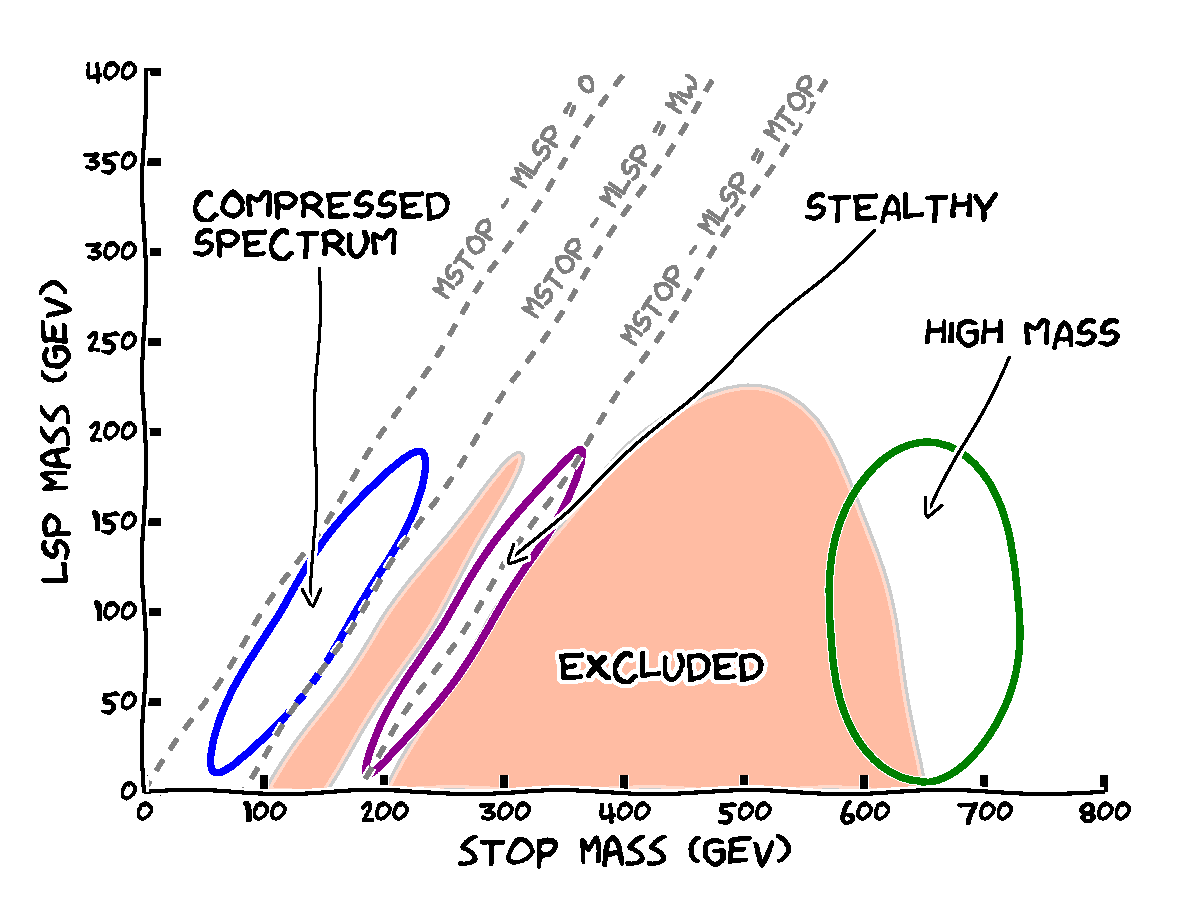
\includegraphics[width=0.8\textwidth]{figures/razor_motivation/story_boost_motivation}
  \caption{General form of the exclusion limits for direct stop production on the
($m_{\stopone},m_{\lsp}$) plane. The red shaded area is the approximate region that has been
excluded by a range of searches. The three colored ellipses indicate the regions that are hard to
probe: the compressed spectra, stealthy top squark scenario and high mass top squarks.
  \label{fig:boost_story_motivation}}
\end{figure}

\paragraph{Compressed scenario}
In general, models with mass spectra featuring small mass splittings are called \textit{compressed
scenarios} or \textit{compressed spectra}. This case thus corresponds to the left-most gap in
Fig.~\ref{fig:boost_story_motivation}, where $\Delta m$ is very small, smaller than the $\W$ boson
mass in particular. 
In this scenario, the top squark decays to the LSP and other soft decay products, either resulting
from the loop-induced decay $\stopone \rightarrow c \lsp$, or from the four-body decay $\stopone
\rightarrow \cPqb f \bar{f} \lsp$. These soft decay products, jets and/or leptons, are difficult to
detect. They are hard to reconstruct, and when reconstructed they often fall below the \pt
thresholds that define the objects. 
Therefore, in order to be sensitive to such processes, one should not rely on the presence of
these objects, but rather on something else, such as the presence of jets from initial state
radiation (ISR). Both ATLAS and CMS have performed searches using this
technique~\cite{CMS-PAS-SUS-13-009,Aad:2014nra}. 

\paragraph{Stealthy stop scenario}
The scenarios where $\Delta m\,{\approx}\, m_t$, are often referred to as \textit{stealthy}
scenarios. The reason for this is that when $\Delta m$ approaches the top mass, the signature of
top squark production is very similar to that of standard model $t\bar{t}$ production,
which has a much higher cross section. Consequently, the signal from direct stop production is
hidden underneath a much larger $t\bar{t}$ background. An alternate way to approach stealthy stops
is, for instance, to assume that the heavy top squark $\stoptwo$ is also accessible at the LHC, and
decays to the $\stopone$ via either a Higgs or $\cPZ$ boson~\cite{Khachatryan:2014doa}. This
results in a longer decay chain, which provides extra handles, such as additional $\cPqb$ quarks or
leptons. 

\paragraph{High mass scenario}
The last gap that is present in the sensitivity of searches for the direct production of top squark
pairs, is the high mass region. In this region the signature is actually very striking, with
usually large hadronic activity and/or missing transverse momentum. The problem lies in the rather
low expected cross section for direct stop production at 8\TeV. We would need much more data than
the $20\fbinv$ that is available to detect this process. 
Of course, with the restart of the LHC at 13\TeV centre-of-mass energy fast approaching, we can
expect to close part of this gap very soon.

\paragraph{}
Apart from the approaches mentioned above, there is another option to tackle the compressed and
stealthy scenarios, namely, looking for top squarks in gluino decays. This is exactly the focus of
the razor boost analysis. 
Specifically, we consider gluino pair production in which the gluino decays to a top squark and a
top quark, $\tilde{g} \rightarrow t \stopone$. In the models considered, largely motivated by
natural supersymmetry, the gluino has a mass around 1-1.5 \TeV and the lighter top squark has a mass
of a few hundred \GeV. Owing to the significant mass gap presumed to exist between the gluino and
the top squark, the top quark from the gluino to top squark decay will receive a large boost.  
The top squark then decays to $c \lsp$ for small $\Delta m$, or to $t \lsp$ for $\Delta m
\,{\approx}\, m_t$. Four-body decays of the top squark are not considered here. 

The simplified models (see Section~\ref{sec:susy_sms} for more information) corresponding to the
decays $\tilde{g} \rightarrow t \stopone$, followed by either $\stopone \rightarrow c \lsp$ or
$\stopone \rightarrow t \lsp$, are called \textit{T1ttcc} and \textit{T1t1t}, respectively, and
illustrated in the diagrams in Fig.~\ref{fig:T1ttcc_T1t1t_diagrams}. For comparison we show in
Fig.~\ref{fig:T2tt_diagram} the diagram for the \textit{T2tt} simplified model, corresponding to
direct top squark production in which the top squark decays to $t \lsp$. 

As the analysis described in this thesis is the first analysis within CMS to explicitely probe
gluino-mediated production of top squark pairs decaying as $\stopone \rightarrow c \lsp$, it
provides new information about the viability of natural SUSY. 

\begin{figure}
  \centering
  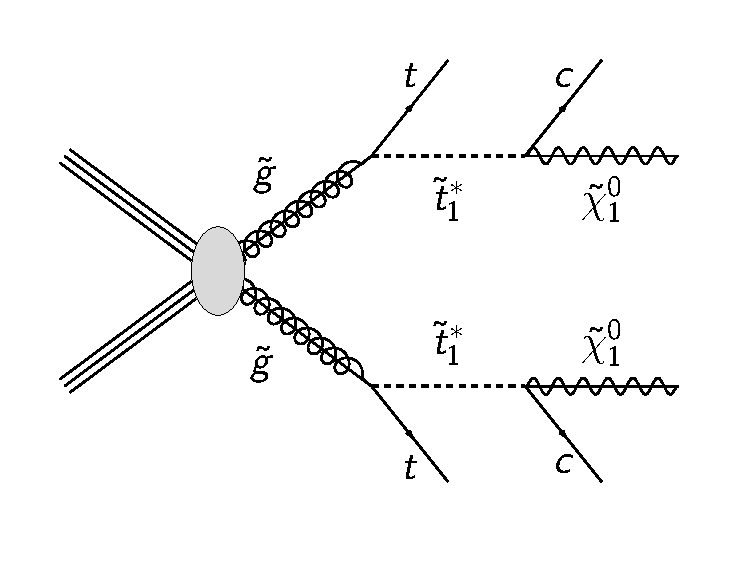
\includegraphics[width=0.48\textwidth,clip=true,trim=0 0.7cm 0 0]
{figures/razor_interpretation/T1ttcc}
  ~
  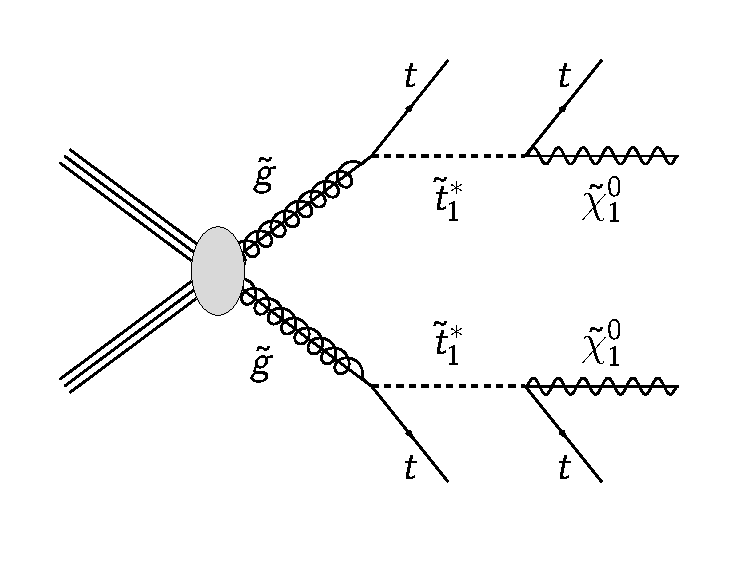
\includegraphics[width=0.48\textwidth,clip=true,trim=0 0.7cm 0 0]
{figures/razor_interpretation/T1t1t}
  \caption{Diagram illustrating the T1ttcc (left) and T1t1t (right) simplified models.
  \label{fig:T1ttcc_T1t1t_diagrams}}
\end{figure}

\begin{figure}
  \centering
  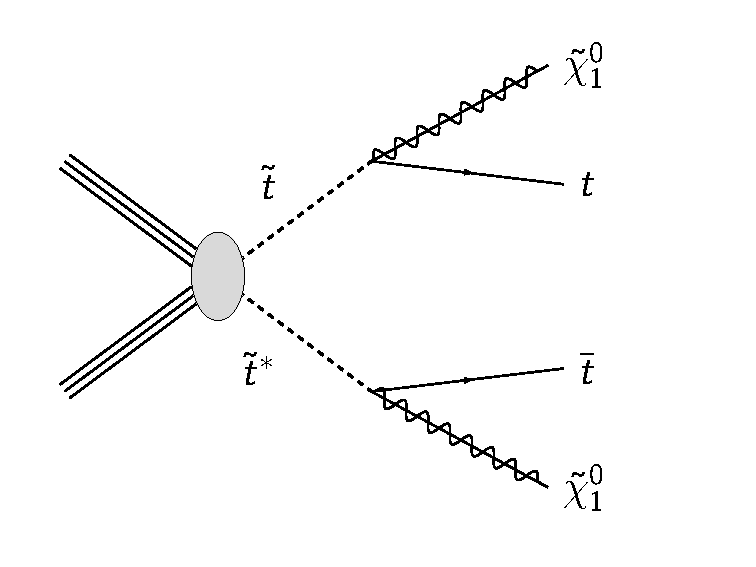
\includegraphics[width=0.48\textwidth,clip=true,trim=0 0.7cm 0 0]{figures/razor_motivation/T2tt}
  \caption{Diagram illustrating the T2tt simplified model.
  \label{fig:T2tt_diagram}}
\end{figure}





\section{General strategy \label{sec:boost_strategy}}

% control regions, transfer factors
% binning in razor variables
% statistical treatment and systematic uncertainties


In light of the discussion in Section~\ref{sec:boost_motivation}, it is expected that boosted top
quarks are a promising signature of new physics involving a massive gluino decaying to a relatively
light top squark.
Boosted objects with high transverse momentum are characterized by merged decay products
separated by $ \Delta R \,{\sim}\, 2m/\pt$\footnote{Considering a heavy object $\W$ with mass $M$
that decays to two massless particles $a$ and $b$, we find $M^2 = 2 p_a \cdot p_b = 2 E_a E_b (1
- \cos{\theta_{ab}})$. Using small angle approximation this becomes $M^2 = E_a E_b
\theta_{ab}^2$. Assigning half of the $\W$ energy to both $a$ and $b$ results in $M^2 =
\frac{1}{4} E_\W^2 \theta_{ab}^2$. Translating this relation into the transverse plane, we get
$\Delta R = \frac{2 M}{\pt^\W}$.}, 
where $m$ and $\pt$ denote the mass and transverse momentum of the mother particle, and $\Delta R$
is given in terms of azimuthal angle $\phi$ and pseudorapidity $\eta$ as $\Delta R = \sqrt{\Delta
\phi^2 + \Delta \eta^2}$.
For a separation of $\Delta R = 0.5$, a top quark should thus have a momentum of ${\sim}700$\GeV, a
value difficult to reach with proton-proton collisions at 8 TeV. Therefore, in order to increase the
signal efficiency, we consider instead $\W$ bosons from top quark decays, which are required to have
a more accessible $\pt \,{\sim}\, 320$\GeV.  The \pt of the top quark and $\W$ boson at generator
level without applying any selection, is shown in Figs.~\ref{fig:boost_gen_toppt} and
\ref{fig:boost_gen_Wpt} for several signal models, and the SM $t\bar{t}$ process. 
We observe that the average \pt is higher for the signal than for $t\bar{t}$. Requiring the
presence of a boosted $\W$ boson will thus be part of the strategy to reduce the SM background.
Hadronically decaying boosted $\W$ boson candidates will be identified using pruned jet
mass~\cite{Ellis:2009su,Ellis:2009me,Chatrchyan:2013vbb} and a jet substructure observable
called N-subjettiness \cite{Thaler:2010tr}. More details on the $\W$ tagging technique will be given
in Section~\ref{sec:boost_wtag}. 

\begin{figure}[htpb]
\centering
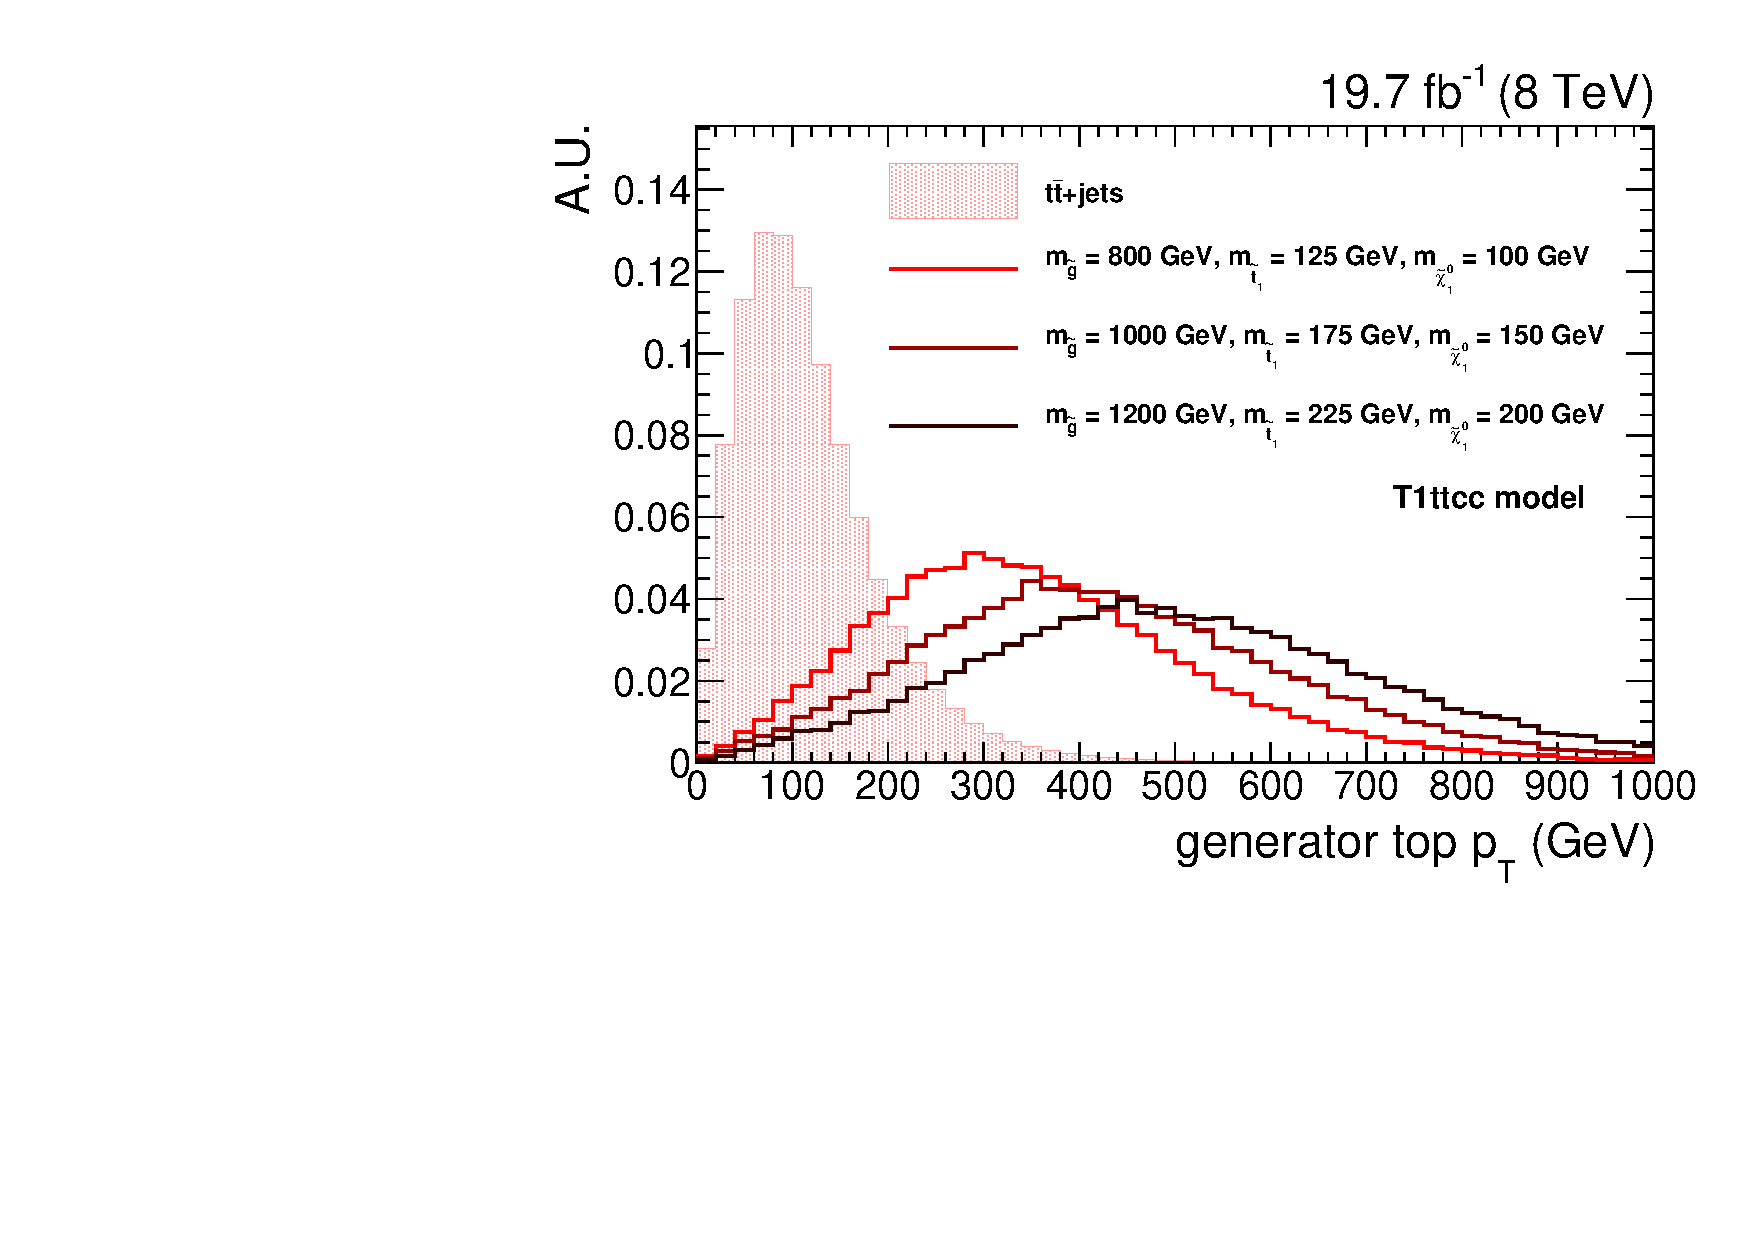
\includegraphics[width=0.48\textwidth]{figures/razor_strategy/T1ttcc_gentoppt}
~
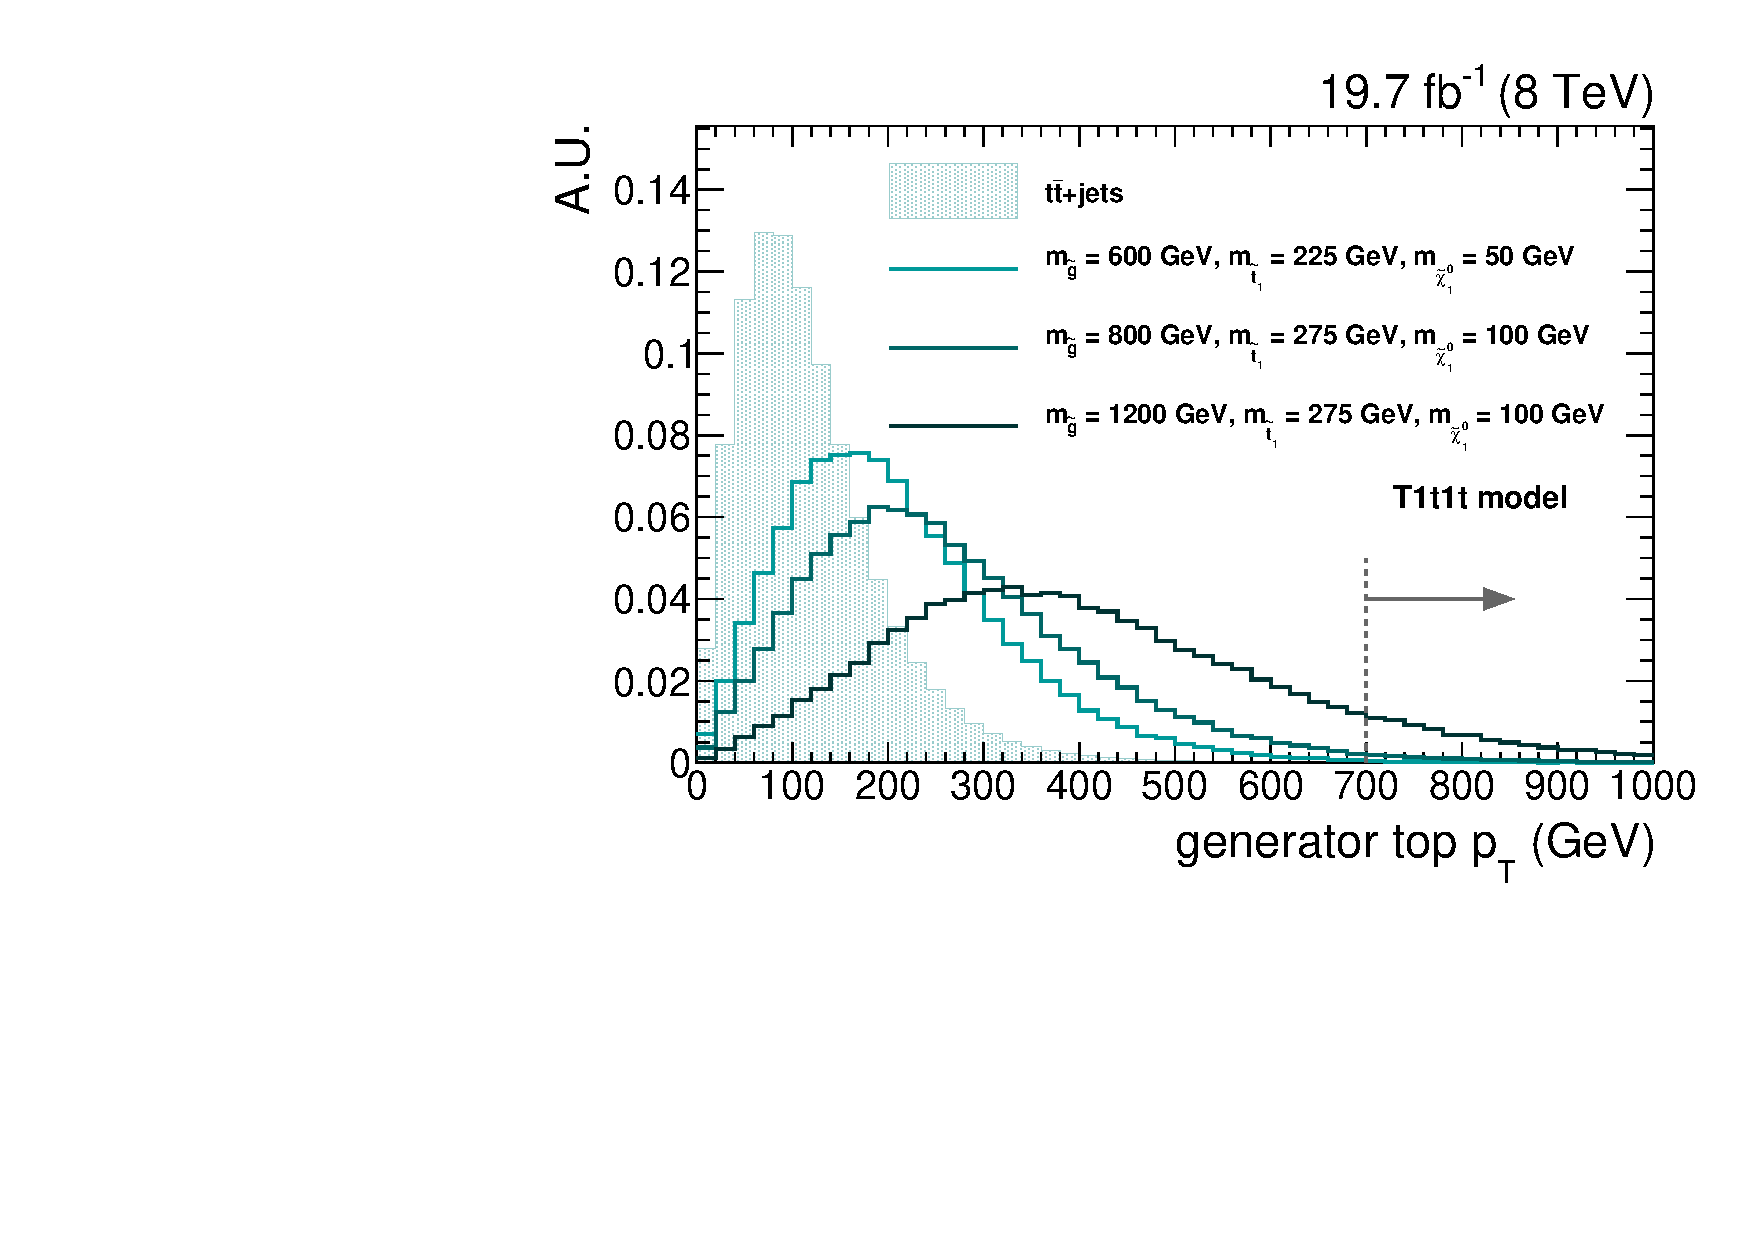
\includegraphics[width=0.48\textwidth]{figures/razor_strategy/T1t1t_gentoppt}
\caption{Generator level top quark \pt for several signal points of the T1ttcc (left) and T1t1t
(right) simplified models. The average \pt increases as the mass splitting increases. The boost of
the top quark is larger for the considered signal models compared to the $t\bar{t}$ background. 
\label{fig:boost_gen_toppt}}
\end{figure}
\begin{figure}[htpb]
\centering
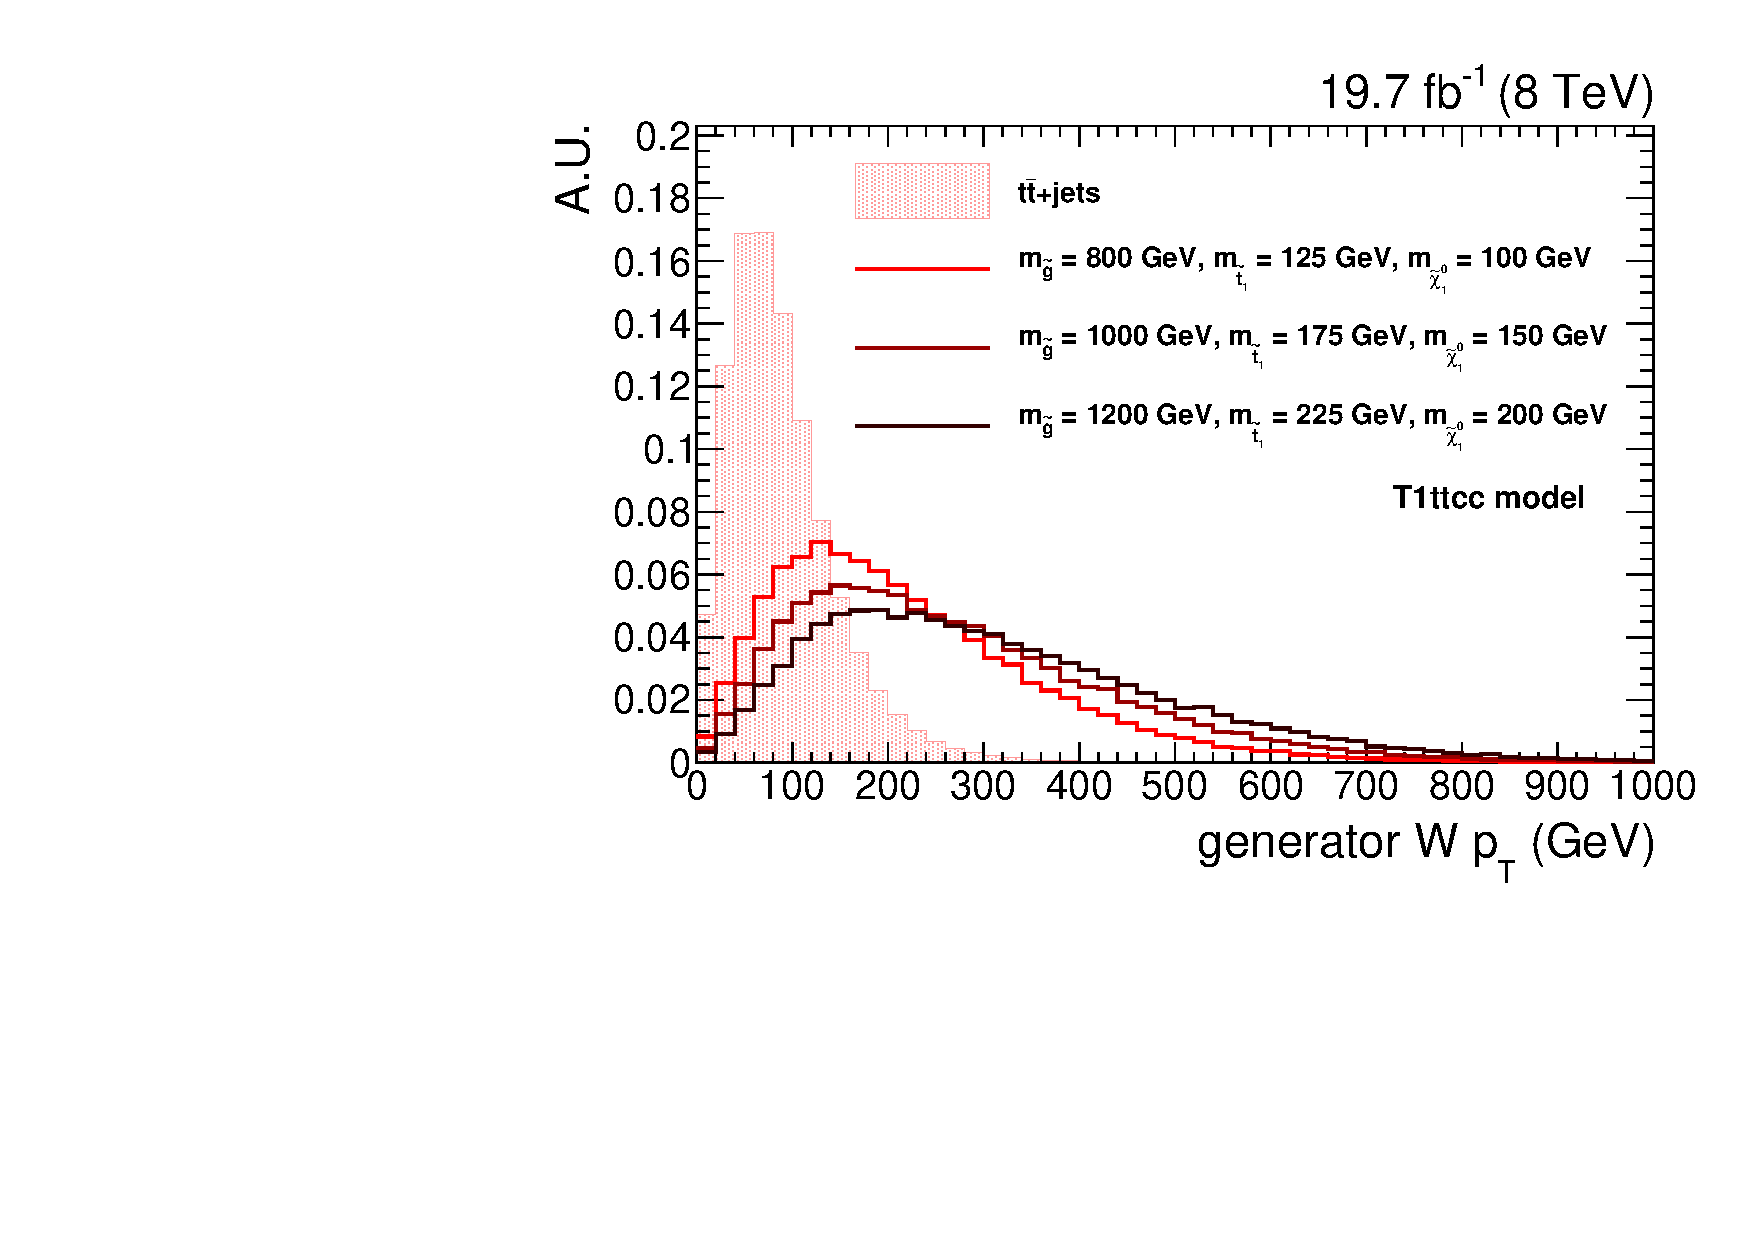
\includegraphics[width=0.48\textwidth]{figures/razor_strategy/T1ttcc_genWpt}
~
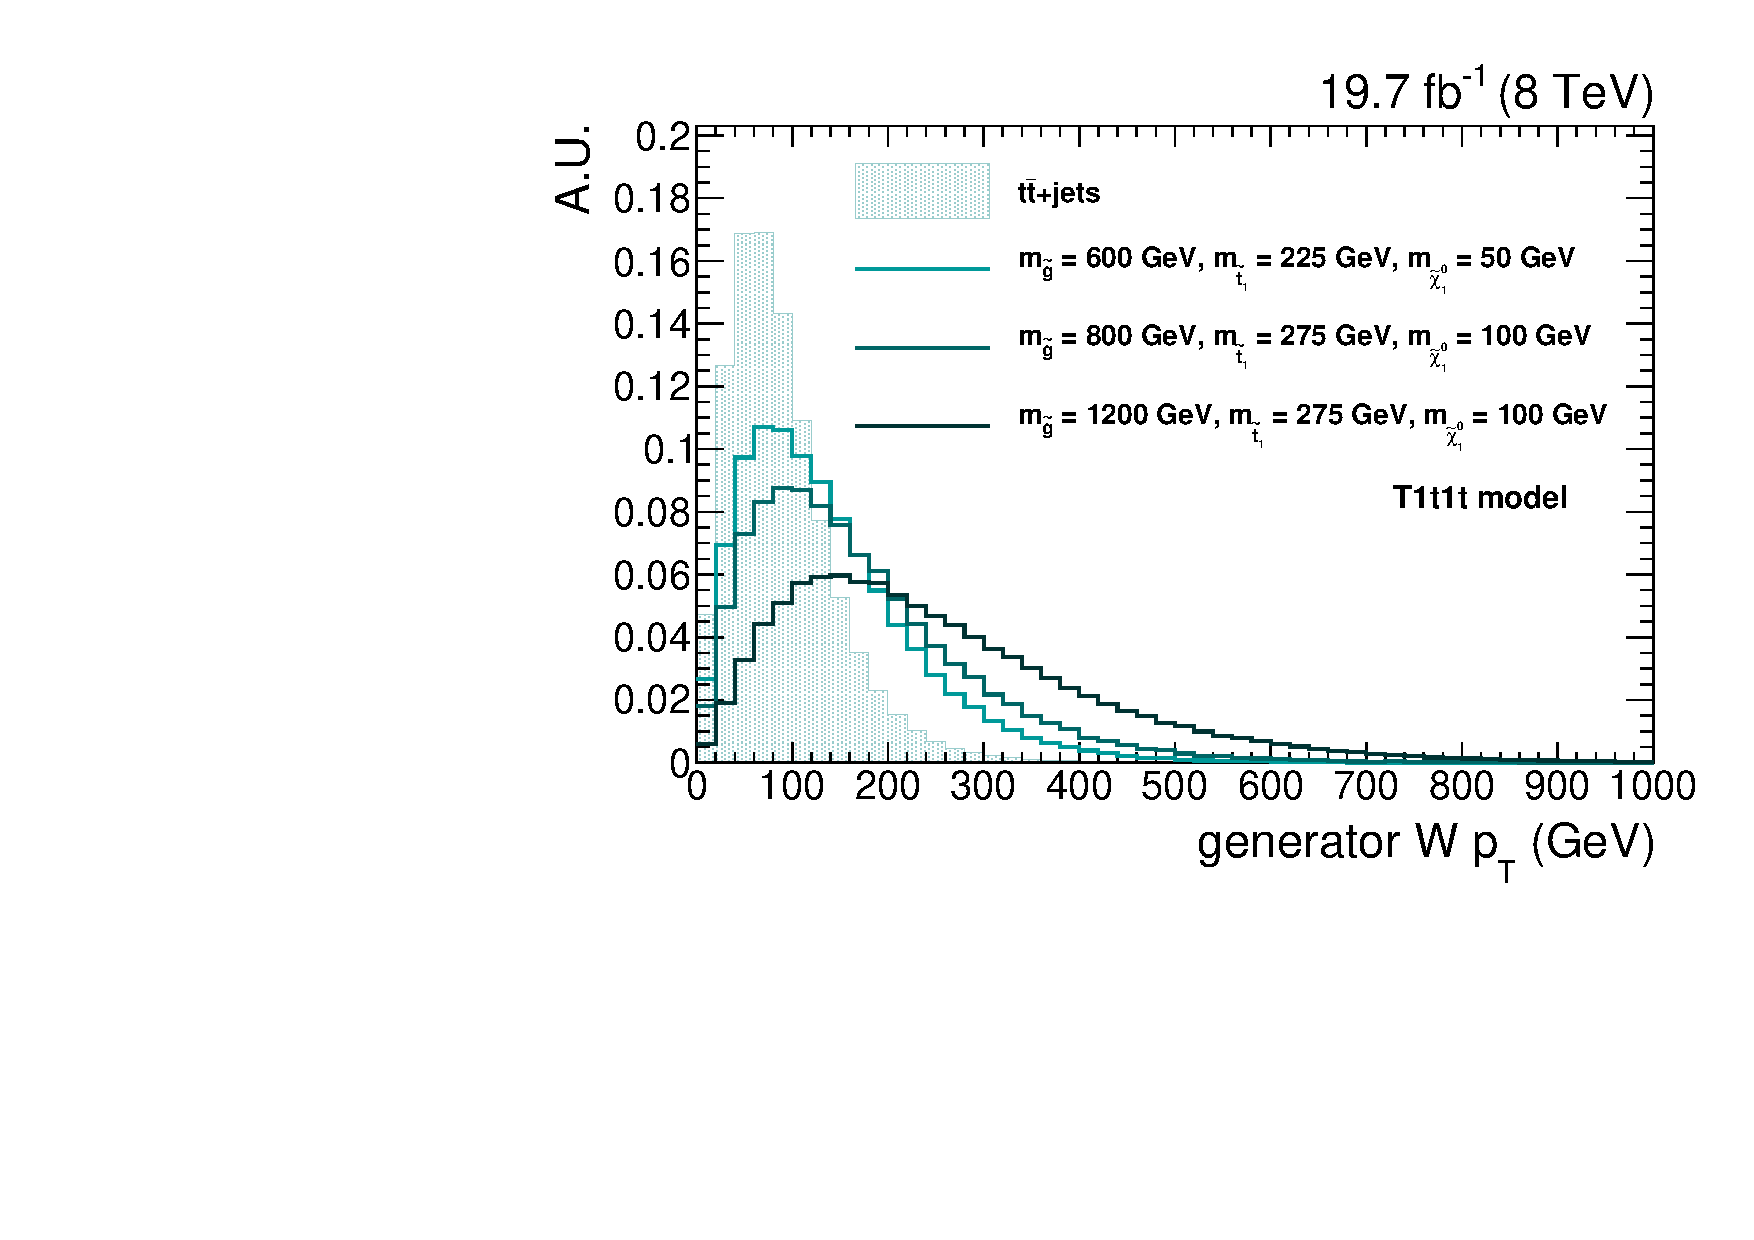
\includegraphics[width=0.48\textwidth]{figures/razor_strategy/T1t1t_genWpt}
\caption{Generator level $\W$ boson \pt for several signal points of the T1ttcc (left) and T1t1t
(right)
simplified models. The average \pt increases as the mass splitting increases. The boost of the $\W$
boson is larger for the considered signal models compared to the $t\bar{t}$ background. 
\label{fig:boost_gen_Wpt}}
\end{figure}

The razor kinematic variables \mr and \rsq, see Section~\ref{sec:boost_razor}, are designed to
discriminate processes with new heavy particles and missing energy from standard model processes.
They will be used in this analysis as the main discriminating variables to search for deviations
from the SM. We will perform the search in 25 search bins across the high $\mr$-high $\rsq$ region,
using hadronic events with at least one boosted $\W$ boson and one jet originating from a $\cPqb$
quark (i.e. $\cPqb$ jet). 

Standard model backgrounds in the signal regions are estimated using observations in control regions
and global scale factors, calculated from simulated data, that relate the number of events in one
region to that in another. 
Three control regions, $Q$, $W$, and $T$, are defined to select high-purity samples of multijet,
$\W(\rightarrow \ell\nu)+$jets and $t\bar{t}$ processes, respectively.  
The background estimation method uses a likelihood-based approach, with a simultaneous sampling
of systematic uncertainties which fully takes into account any correlations automatically.
An overview of the different regions and how they are related, including for the control regions
which background parameters of the likelihood each region constrains, is shown in
Fig.~\ref{fig:boost_flowchart}. For the full explanation of the background estimation method, I
refer to Section~\ref{sec:boost_likelihood}. 

\begin{figure}[p]
  \centering
  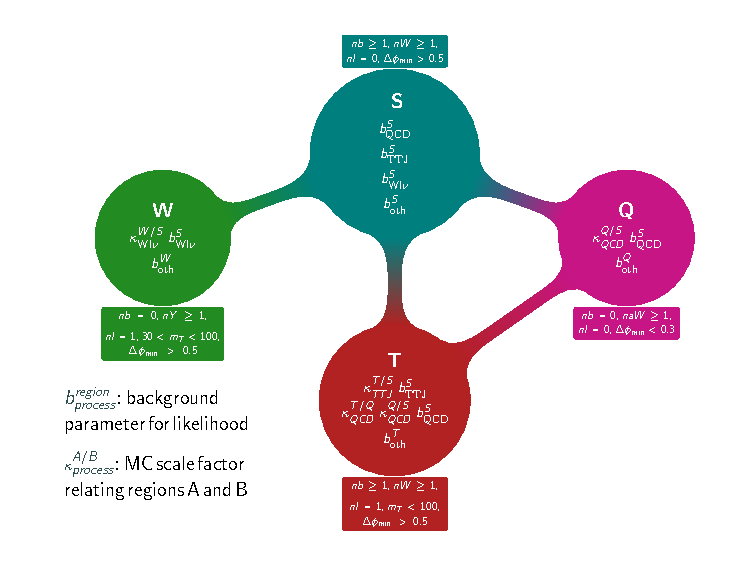
\includegraphics[width=\textwidth]{figures/razor_strategy/BoostFlowChart_noZ}
  \caption{Definition of, and relationship between, the signal ($S$) and control ($Q,T,W$) regions
and their relationship to the bin-by-bin background parameters
$b^{\textrm{region}}_{\textrm{process}}$ for a given region and background process, as well as the
four global scale factors $\kappa^{A/B}_{\textrm{process}} = \sum_i b^A_{\textrm{process}, MC, i} /
\sum_i b^B_{\textrm{process}, MC, i}$, where the sum is over all 25 (\mr,\rsq) bins of the simulated
data. 
The total expected background, per bin, is the sum of the terms shown for each region. Furthermore,
associated with each bin of each region is an observed count $N^{\textrm{region}}$, a simulated
count $N^{\textrm{region}}_{\textrm{process}, MC}$, and a count $N^{\textrm{region}}_{oth, MC}$
equal to the sum of the smaller backgrounds, with associated parameter $b^{\textrm{region}}_{oth}$.
  \label{fig:boost_flowchart}}
\end{figure}

% 
% \begin{figure}[htbp]
% \centering
% \includegraphics[width=0.49\textwidth]{figures/T1ttcc/Signal_comparison_T1ttcc_gen_toppt}
% \includegraphics[width=0.49\textwidth]{figures/T1t1t/Signal_comparison_T1t1t_gen_toppt}
% \caption{Generator top \pt for several signalpoints of the T1ttcc (left) andT1t1t (right)
% simplified
% models.
% \label{fig:gen_toppt}}
% \end{figure}


\section{Razor variables \label{sec:boost_razor}}

%%%%%%%%%%%%%%%%%%%
% razor variables
%%%%%%%%%%%%%%%%%%%

% add full derivation
% plots of signal and background

Many extensions of the Standard Model (see chapter~\ref{chap:beyond_standard_model}) predict the 
existence of new particles, which can be pair-produced in the proton-proton collisions at the LHC. 
Some of those theories introduce an extra symmetry, such as the R-parity in supersymmetry. A
consequence of this symmetry is that the lightest BSM particle must be stable, as it cannot decay
to SM particles only. This lightest BSM particle, called LSP in supersymmetric theories, is weakly
interacting, and escapes the detector unseen. 

This general property leads us to a generic class of new physics signatures in which a heavy
particle is pair-produced, and decays into visible, i.e. interacting with our detector, SM
particles, and an invisible LSP. This signature is illustrated in figure~\ref{fig:razor_signature}.

\begin{figure}[htb]
  \centering
  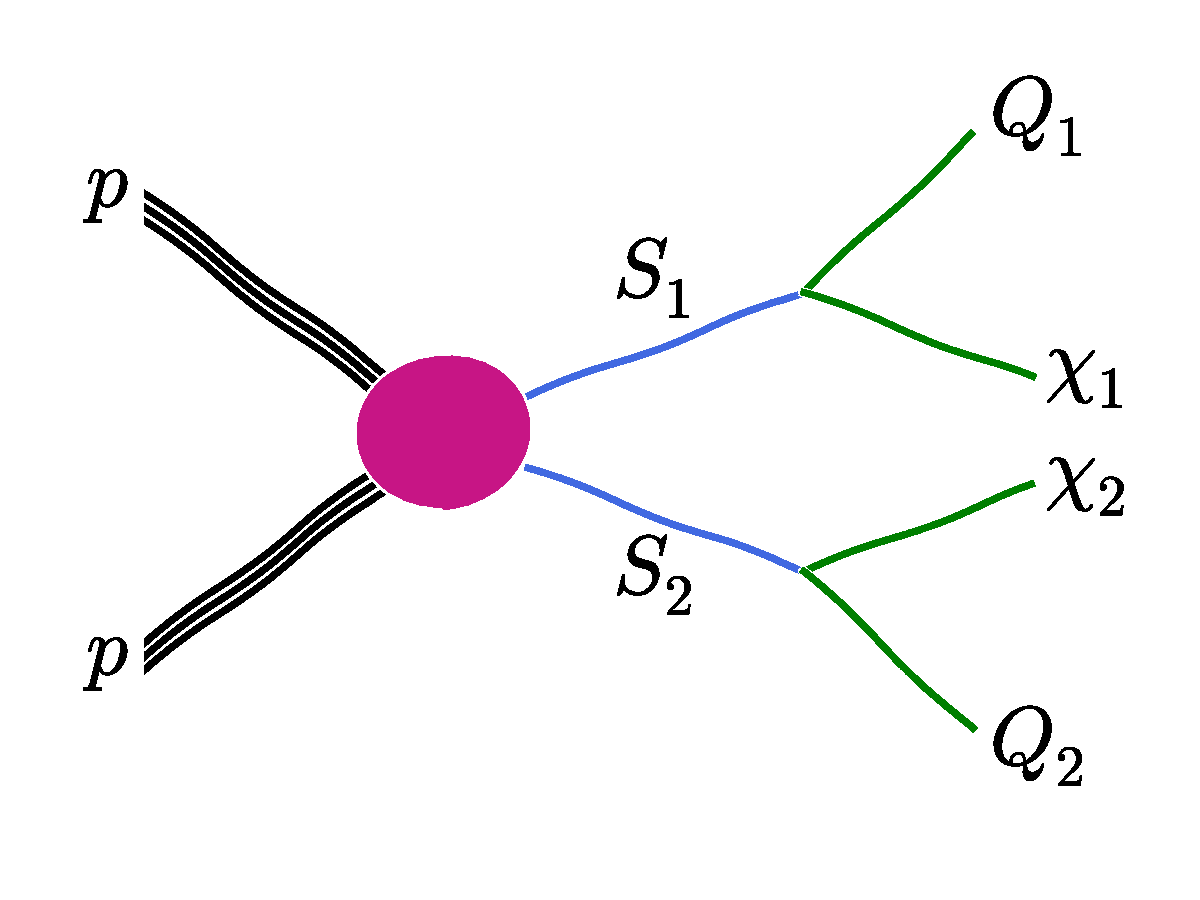
\includegraphics[width=0.6\textwidth,clip=true,trim=0 1.8cm 0
0.8cm]{figures/razor_variables/signature} 
  \caption{Generic new physics signature. Two massive new particles, $S_1$ and $S_2$, are produced
in $\Pp\Pp$ collisions at the LHC, and consequently decay to a visible system $Q_i$ and an invisible
system $\chi_i$. \label{fig:razor_signature}}
\end{figure}

Several kinematical variables targetting this topology have been
developed~\cite{Lester:1999tx,Barr:2003rg,Randall:2008rw,Polesello:2009rn,Bai:2012gs}.
% TODO add citations here
Most of these variables rely on the presence of the invisible LSP's. This causes the visible system
to deviate from a di-jet topology, resulting in possibly large missing transverse momentum, altered
angular distributions, et cetera. All of this can be used to distinguish the sought-after signal
from the known background processes. 
Unfortunately, the ultimate goal of reconstructing the masses of the new particles cannot be
attained. Because of the escaping LSP's, there is simply not enough information available to fully
constrain the problem. What we can do, however, is approximate the mass scale of the new physics
particles. Often times this results in variables that exhibit a kinematic edge. 
The \textit{razor variables} \cite{rogan,Rogan:1557072,Chatrchyan:2011ek,Chatrchyan:2014goa} are no
exception in this regard. One advantage the razor variables have over many other variables, is that
they also reconstruct the mass scale as a peak, in addition to a kinematic edge. 
In what follows I will derive the two razor variables, denoted \mr and \rsq, which use longitudinal
and transverse event information, respectively, to estimate a characteristic mass scale associated
with the new particles. At the end of this section I will briefly show how the razor variables are
used in the razor boost analysis. 

% explain reference frames

\subsection{Kinematical configuration and notation \label{sec:razor_notation}}

Let's again consider figure~\ref{fig:razor_signature}. For simplicity, we will assume that the
produced particles $S_1$ and $S_2$ undergo a two-body decay. Each $S_i$ decays to a visible,
standard model particle $Q_i$, and a particle $\chi_i$ that escapes the detector. 
We assume a symmetric decay chain, with the following relations for the masses of the different
particles,
\begin{alignat}{3}
  M_{S_1} &= M_{S_2} &&= M_S \label{eq:equal_S_masses}\\
  M_{\chi_1} &= M_{\chi_2} &&= M_{\chi} \label{eq:equal_chi_masses}\\
  M_{Q_1} &= M_{Q_2} &&= 0 \label{eq:no_Q_masses}
\end{alignat}

There are four relevant reference frames for our goal of determining a characteristic mass scale
of the new physics process under consideration. The following paragraphs will go through each of
these and define the notations that will be used, as well as deriving relations between several
variables. 

\paragraph{$S_1$ rest frame} 
From basic two-body decay kinematics it follows that the $Q_1$ and $\chi_1$ particles are produced
back to back, with equal magnitude of momentum, in the rest frame of the $S_1$ particle. This is
illustrated in figure~\ref{fig:razor_S1_rest_frame}. 

\begin{figure}[htpb]
  \centering
  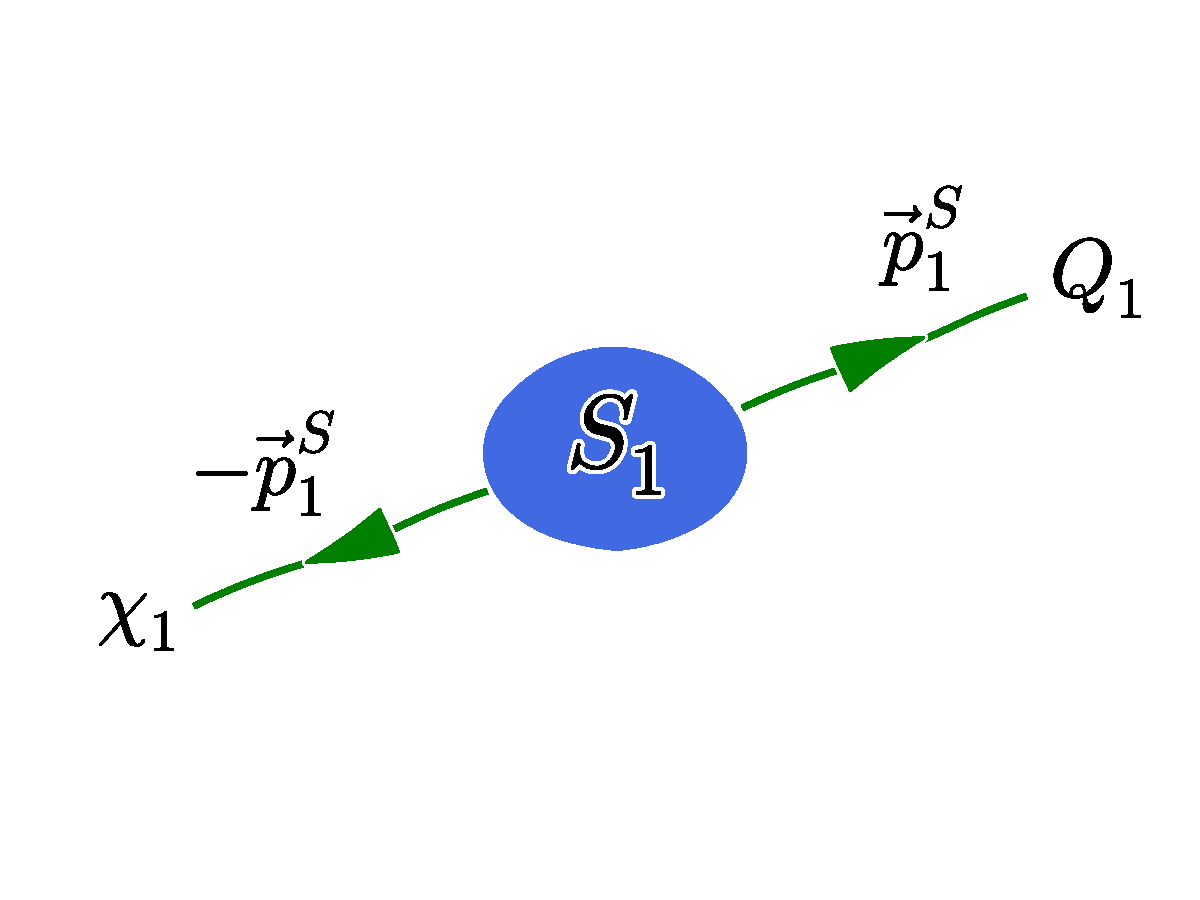
\includegraphics[width=0.6\textwidth,clip=true,trim=0 4cm 0
3cm]{figures/razor_variables/rest_frame}
  \caption{Configuration of the $S_1$ rest frame. The decay products $Q_1$ and $\chi_1$ are
produced back to back with momenta $\vec{p}^S_1$ and $-\vec{p}^S_1$, respectively. 
\label{fig:razor_S1_rest_frame}}
\end{figure}

We can compute the magnitude of this momentum in terms of the new particle masses. To do this we
start from the four-vectors of the $Q_1$ and $\chi_1$ particles in the $S_1$ rest frame, 
\begin{alignat}{6}
  P[Q_1]    &\equiv q_1^S   &&= \{ E^S_{Q_1}, \vec{q}^S_1\} , \\
  P[\chi_1] &\equiv \nu_1^S &&= \{ E^S_{\chi_1}, \vec{\nu}^S_1\} .
\end{alignat}
Conservation of energy in the $S_1$ rest frame leads to 
\begin{equation}
  E^S_{Q_1} + E^S_{\chi_1} = M_S . \label{eq:razor_conservation_energy}
\end{equation}
This can also be expressed as
\begin{equation}
  \sqrt{M_{Q_1}^2 + (\vec{q}^S_1)^2 } + \sqrt{M_{\chi_1}^2 + (\vec{\nu}^S_1)^2} = M_S .
\end{equation}
Using Eq.~\ref{eq:equal_chi_masses} and Eq.~\ref{eq:no_Q_masses} (massless $Q_1$), and the equal
momenta $|\vec{q}^S_1| = |\vec{\nu}^S_1| = |\vec{p}^S_1|$, the above can be simplified as
\begin{align}
  |\vec{p}^S_1|   &= M_S - \sqrt{M_{\chi}^2 + (\vec{p}^S_1)^2} \\
  (\vec{p}^S_1)^2 &= M_S^2 - 2 M_S \sqrt{M_{\chi}^2 + (\vec{p}^S_1)^2} + M_{\chi}^2 +
(\vec{p}^S_1)^2 \\
  2 M_S \sqrt{M_{\chi}^2 + (\vec{p}^S_1)^2} &= M_S^2 + M_{\chi}^2 \\
  4 M_S^2 (\vec{p}^S_1)^2 &= (M_S^2)^2 + 2 M_S^2 M_{\chi}^2 + (M_{\chi}^2)^2 - 4 M_S^2
M_{\chi}^2 \\
  (\vec{p}^S_1)^2 &= \frac{(M_S^2 -M_{\chi}^2 )^2}{4 M_S^2} .
\end{align}

We thus find for the magnitude of the momentum of $Q_1$ and $\chi_1$ in the $S_1$ rest frame
\begin{equation}
  |\vec{p}^S_1| = \frac{M_S^2 -M_{\chi}^2}{2 M_S} \equiv \frac{M_\Delta}{2} ,
\label{eq:razor_p_S1_rest_frame}
\end{equation}
where we have defined the characteristic scale $M_\Delta$. This scale is exactly the scale we are
interested in. The goal of the \textbf{razor variables} is to \textbf{express $M_\Delta$ using lab
frame quantities only}. To succeed in this effort, we will have to make several, physics-motivated,
approximations. These will remove the unknown degrees of freedom, and are further explained in
sections~\ref{sec:razor_mr} and \ref{sec:razor_r2}. 

The energy of the $Q_1$ and $\chi_1$ particles can also be computed easily. 
From the masslessness of $Q_1$, we immediately find using Eq.~\ref{eq:razor_p_S1_rest_frame}
\begin{equation}
  E^S_{Q_1} = |\vec{p}^S_1| = \frac{M_\Delta}{2}. \label{eq:razor_E_Q1}
\end{equation}
To compute $E^S_{\chi_1}$, we substitute Eq.~\ref{eq:razor_E_Q1} in 
Eq.~\ref{eq:razor_conservation_energy}, and find 
\begin{align}
  E^S_{\chi_1} &= M_S - |\vec{p}^S_1|\\
	       &= M_S - \frac{M_S^2 -M_{\chi}^2}{2 M_S} \\
	       &= \frac{2M_S^2 - M_S^2 + M_{\chi}^2}{2 M_S} \\
	       &= \frac{M_S^2 + M_{\chi}^2}{2 M_S} \\
	       &= \frac{M_S^2 - M_{\chi}^2}{2 M_S} \frac{M_S^2 + M_{\chi}^2}{M_S^2 - M_{\chi}^2} .
%               &= \frac{M_\Delta}{2} R_{S\chi}
\end{align}

We can summarize the four-momenta of $Q_1$ and $\chi_1$ in the $S_1$ rest frame as
\begin{align}
  q_1^S   &= \frac{M_\Delta}{2} \{ 1, \vec{u}_1\} , \\  
  \nu_1^S &= \frac{M_\Delta}{2} \{ R_{S\chi}, -\vec{u}_1\} ,
\end{align}
with $$R_{S\chi} = \frac{M_S^2 + M_{\chi}^2}{M_S^2 - M_{\chi}^2},$$ and $\vec{u}_1$ the unit
vector along the $Q_1$ momentum direction.



\paragraph{$S_2$ rest frame}
The discussion of the $S_2$ rest frame is fully analogous to that of the $S_1$ rest frame. We
again find that
\begin{align}
  q_2^S   &= \frac{M_\Delta}{2} \{ 1, \vec{u}_2\} , \\  
  \nu_2^S &= \frac{M_\Delta}{2} \{ R_{S\chi}, -\vec{u}_2\} ,
\end{align}
and thus
\begin{equation}
  |\vec{p}^S_1| = |\vec{p}^S_2| = \frac{M_\Delta}{2} . \label{eq:razor_equal_momenta}
\end{equation}


\paragraph{Center-of-mass frame}
In the center-of-mass (CM) frame of the considered $\Pp\Pp$ collision events the particles $S_1$
and $S_2$, which have equal mass (Eq.~\ref{eq:equal_S_masses}), are produced with equal and opposite
velocities $\betaCM$, as illustrated in figure~\ref{fig:razor_CM_frame}. The boost $\betaCM$ is an
indication of how far above threshold the $S_i$ particles are produced, but unfortunately this is
an unknown at hadron colliders. 

\begin{figure}[htpb]
  \centering
  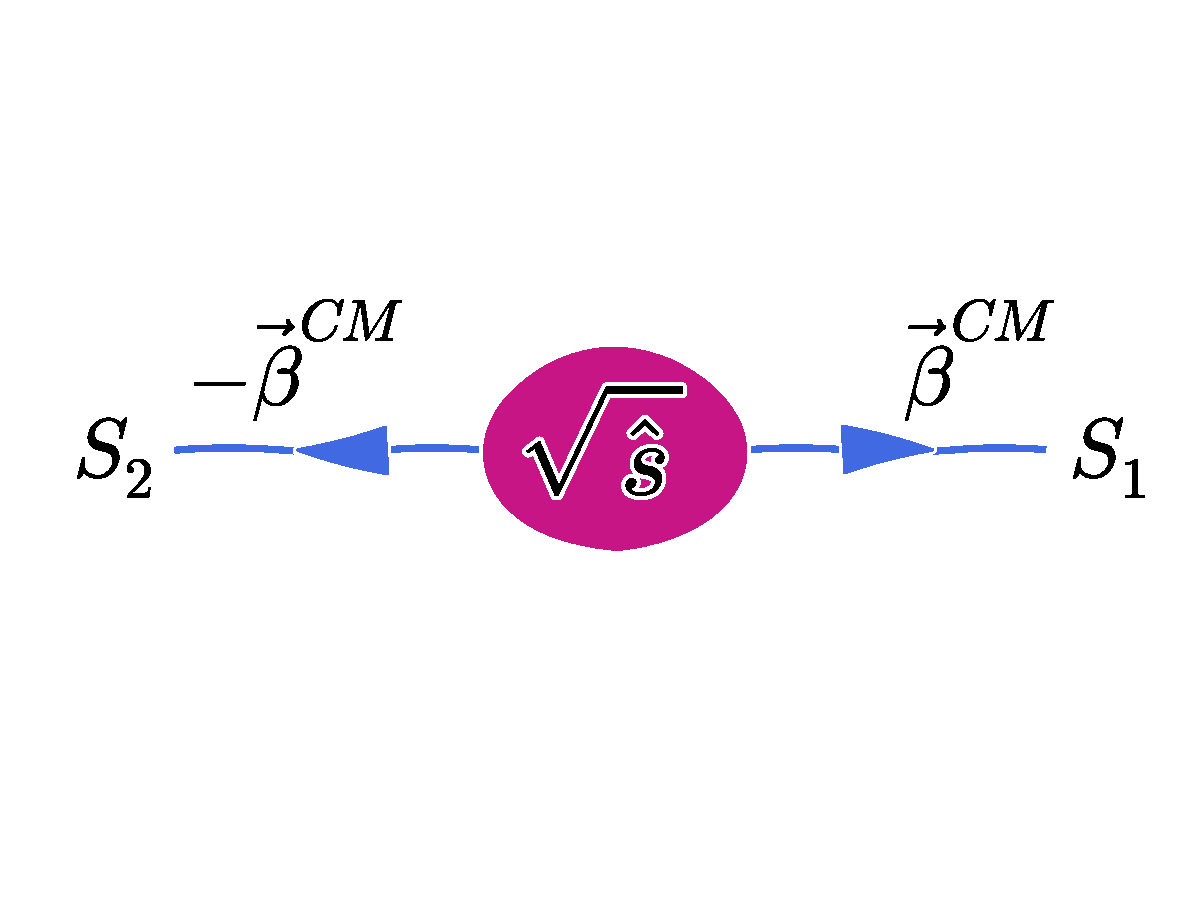
\includegraphics[width=0.6\textwidth,clip=true,trim=0 5.5cm 0
4.5cm]{figures/razor_variables/cm_frame} 
  \caption{Configuration of the center-of-mass frame. The particles $S_1$ and $S_2$ are
produced back to back with velocities $\betaCM$ and $-\betaCM$, respectively. 
\label{fig:razor_CM_frame}}
\end{figure}

To go from the rest frame of $S_1$ ($S_2$) to the CM frame, we need to boost the four-momenta
$q_1^S$ and $\nu_1^S$ ($q_2^S$ and $\nu_2^S$) to the frame travelling at velocity $\betaCM$
($-\betaCM$) with respect to the $S_1$ ($S_2$) rest frame. 
The four-vectors of particles $S_1$ and $S_2$ in the center-of-mass frame are also obtained by
boosting according to $\betaCM$. They can be written as
\begin{alignat}{6}
  P[S_1] &\equiv s^{\textrm{CM}}_1  &&= \{ E^{\textrm{CM}}_{S_1} , \vec{s}^{\textrm{CM}}_{S_1}\} 
&&= M_S \, \gamma^{\textrm{CM}} \, \{ 1 , \betaCM\} , \\ 
  P[S_2] &\equiv s^{\textrm{CM}}_2 &&= \{ E^{\textrm{CM}}_{S_2} , \vec{s}\,^{\textrm{CM}}_{S_2}\}
&&= M_S \, \gamma^{\textrm{CM}} \, \{ 1 , -\betaCM\},  
\end{alignat}
and satisfy the following
\begin{equation}
  (s^{\textrm{CM}}_1 + s^{\textrm{CM}}_1)^2 = \hat{s} = 4 (\gamma^{\textrm{CM}})^2 M_S^2,
\end{equation}
with $\sqrt{\hat{s}}$ the center-of-mass energy of the collision. 


\paragraph{Lab frame}
The lab frame is the frame where we make our measurements, and is related to the CM frame by a
boost $\vec{\beta}^{\textrm{lab}}$. We can decompose this boost into a transverse and longitudinal
part as $\vec{\beta}^{\textrm{lab}} = (\vec{\beta}_T,\vec{\beta}_z)$. 
The four-momenta of the $S_i$, $Q_i$ and $\chi_i$ particles are denoted by $s^{\textrm{lab}}_i$,
$q^{\textrm{lab}}_i$, and $\nu^{\textrm{lab}}_i$ respectively. 



\subsection{Derivation of \texorpdfstring{\mr}{MR} \label{sec:razor_mr}}

As mentioned in the previous section, our goal is to express the characteristic scale $M_\Delta$
using lab frame quantities only. Because the problem is kinematically underconstrained, we will
need to make some approximations as we work our way from the lab frame to the $S_i$ rest frame,
reversing the boosts $\vec{\beta}^{\textrm{lab}}$ and $\betaCM$ as we go along. 

The models of new physics that we aim to target with the razor variables all predict that the new
particles are heavy. This prediction is the basis of the two approximations we will be making. 

\begin{enumerate}
  \item If $M_S$ is large compared to $\sqrt{s}$, then the particles $S_1$ and $S_2$ will be
produced near the $\sqrt{\hat{s}} = 2 M_S$ threshold. This means that $\gamma^{\textrm{CM}} \approx
1$. We will thus assume that $\gamma^{\textrm{CM}} = 1$, which means that $\betaCM \rightarrow 0$. 
The CM frame is thus equal to both $S_i$ rest frames after this first approximation. 
  \item The transverse boost between lab frame and CM frame can be approximated by 
  \begin{equation}
    |\vec{\beta}_T| \approx \frac{p_T^{ISR}}{\sqrt{\hat{s}}} \lesssim \frac{p_T^{ISR}}{2M_S},
  \end{equation}
  where $p_T^{ISR}$ is the magnitude of the vectorial sum of the transverse momentum of the initial
state radiation. For large values of $M_S$ we find $\vec{\beta}_T \ll 1$. We thus assume that
$\vec{\beta}_T \rightarrow 0$, and thus $\vec{\beta}^{\textrm{lab}} \rightarrow \vec{\beta}_z$.
\end{enumerate}
The results of these two approximations is that we only need a longitudinal boost $\vec{\beta}_z$
to take us from the lab frame to the approximate $S_i$ rest frames. 
In this so-called \textit{rough-approximation frame}, or \textit{R-frame}, we have that
\begin{alignat}{4}
  |\vec{q}^R_1|         &= |\vec{q}^R_2| &&= \frac{M_\Delta}{2} , \\
  \textrm{or } E_{Q_1}^R &= E_{Q_2}^R     &&= \frac{M_\Delta}{2}.
\label{eq:razor_equal_energy_R_frame}
\end{alignat}
cf. Eq.~\ref{eq:razor_equal_momenta}. Using this constraint, we can compute the boost $\beta^R$
that will take us from the lab frame to the R-frame. We start from the basic Lorentz
transformations for energy and momentum, 
\begin{align}
  E_{Q_i}^R      &= \gamma^R \left( E_{Q_i}^{\textrm{lab}} - \beta^R \vec{q}_{iz}^{\textrm{lab}}
\right) , \\
  \vec{q}_{iz}^R &= \gamma^R \left( \vec{q}_{iz}^{\textrm{lab}} - \beta^R E_{Q_i}^{\textrm{lab}}
\right) .
\end{align}
Using Eq.~\ref{eq:razor_equal_energy_R_frame} we find
\begin{equation}
  E_{Q_1}^{\textrm{lab}} - \beta^R \vec{q}_{1z}^{\textrm{lab}} = E_{Q_2}^{\textrm{lab}} - \beta^R
\vec{q}_{2z}^{\textrm{lab}} ,
\end{equation}
and thus for the boost $\beta^R$
\begin{equation}
  \beta^R = \frac{E_{Q_1}^{\textrm{lab}} - E_{Q_2}^{\textrm{lab}}}{\vec{q}_{1z}^{\textrm{lab}} -
\vec{q}_{2z}^{\textrm{lab}}} . \label{eq:razor_beta_R}
\end{equation}
The Lorentz factor $\gamma^R$ can be expressed as
\begin{align}
  \gamma^R &= \frac{1}{\sqrt{1 - (\beta^R)^2}} \\
	   &= \frac{1}{\sqrt{1 - \left( \frac{E_{Q_1}^{\textrm{lab}} -
E_{Q_2}^{\textrm{lab}}}{\vec{q}_{1z}^{\textrm{lab}} -
\vec{q}_{2z}^{\textrm{lab}}} \right)^2}} \\
           &= \frac{ \vec{q}_{1z}^{\textrm{lab}} - \vec{q}_{2z}^{\textrm{lab}} }{\sqrt{ \left(
 \vec{q}_{1z}^{\textrm{lab}} - \vec{q}_{2z}^{\textrm{lab}} \right)^2 - \left(
 E_{Q_1}^{\textrm{lab}} - E_{Q_2}^{\textrm{lab}}\right)^2 }} \label{eq:razor_gamma_R}
\end{align}

We now define \mr as
\begin{equation}
  \mr \equiv 2 |\vec{q}^R| = M_\Delta .
\end{equation}
It is interesting to note that \mr is invariant under longitudinal boosts. Using
Eq.~\ref{eq:razor_beta_R} and Eq.~\ref{eq:razor_gamma_R}, we can express \mr using lab frame
quantities only. 

\begin{align}
  \mr &= E_{Q_1}^R + E_{Q_2}^R \\
      &= \gamma^R \left( E_{Q_1}^{\textrm{lab}} + E_{Q_2}^{\textrm{lab}} - \beta^R (
\vec{q}_{1z}^{\textrm{lab}} + \vec{q}_{2z}^{\textrm{lab}}) \right) \\
      &= \frac{\left( \vec{q}_{1z}^{\textrm{lab}} - \vec{q}_{2z}^{\textrm{lab}}\right) 
               \left( E_{Q_1}^{\textrm{lab}} + E_{Q_2}^{\textrm{lab}} - \frac{E_{Q_1}^{\textrm{lab}}
- E_{Q_2}^{\textrm{lab}}}{\vec{q}_{1z}^{\textrm{lab}} - \vec{q}_{2z}^{\textrm{lab}}}
(\vec{q}_{1z}^{\textrm{lab}} + \vec{q}_{2z}^{\textrm{lab}}) \right)}
              { \sqrt{ \left( \vec{q}_{1z}^{\textrm{lab}} - \vec{q}_{2z}^{\textrm{lab}} \right)^2 
                      -\left( E_{Q_1}^{\textrm{lab}} - E_{Q_2}^{\textrm{lab}}\right)^2 }} \\
      &= \frac{\left( \vec{q}_{1z}^{\textrm{lab}} - \vec{q}_{2z}^{\textrm{lab}} \right) 
               \left( E_{Q_1}^{\textrm{lab}} + E_{Q_2}^{\textrm{lab}} \right) 
               - 
               \left( E_{Q_1}^{\textrm{lab}} - E_{Q_2}^{\textrm{lab}} \right)
               \left( \vec{q}_{1z}^{\textrm{lab}} + \vec{q}_{2z}^{\textrm{lab}} \right) }
              { \sqrt{ \left( \vec{q}_{1z}^{\textrm{lab}} - \vec{q}_{2z}^{\textrm{lab}} \right)^2 
                      -\left( E_{Q_1}^{\textrm{lab}} - E_{Q_2}^{\textrm{lab}}\right)^2 }} \\
      &= \frac{2 \left( \vec{q}_{1z}^{\textrm{lab}} E_{Q_2}^{\textrm{lab}} 
                       - \vec{q}_{2z}^{\textrm{lab}} E_{Q_1}^{\textrm{lab}} \right)}
              { \sqrt{ \left( \vec{q}_{1z}^{\textrm{lab}} - \vec{q}_{2z}^{\textrm{lab}} \right)^2 
                      -\left( E_{Q_1}^{\textrm{lab}} - E_{Q_2}^{\textrm{lab}}\right)^2 }}
\end{align}
Our final expression for \mr in lab frame quantities becomes
\begin{equation}
  \mr = 2 \sqrt { \frac{ \left( \vec{q}_{1z}^{\textrm{lab}} E_{Q_2}^{\textrm{lab}} 
                       - \vec{q}_{2z}^{\textrm{lab}} E_{Q_1}^{\textrm{lab}} \right) ^2}
                       { \left( \vec{q}_{1z}^{\textrm{lab}} - \vec{q}_{2z}^{\textrm{lab}}
\right)^2 
                        -\left( E_{Q_1}^{\textrm{lab}} - E_{Q_2}^{\textrm{lab}}\right)^2 }} . 
\end{equation}
As the R-frame is only an approximation of the $S_i$ rest frames, \mr will be distributed around
the characteristic scale $M_\Delta$ with degrading resolution as the Lorentz factor increases. 
More generally, the peak value of \mr scales as $\gamma^{\textrm{CM}}M_\Delta$.

We can use \mr as a way to distinguish signal from background, in particular background from QCD
multijet production. Let's consider QCD dijet production. In the dijet rest frame we have for the
four-momenta of the two jets, $k_1$ and $k_2$
\begin{align}
  k_1 &= \frac{\sqrt{\hat{s}}}{2} \{1, \vec{v}\} ,\\
  k_2 &= \frac{\sqrt{\hat{s}}}{2} \{1, -\vec{v}\},
\end{align}
where $\sqrt{\hat{s}}$ is the center-of-mass energy of the partonic subprocess, and $\vec{v}$ is a
unit vector along the dijet axis. For this type of event, $\mr = \sqrt{\hat{s}}$, and is thus
sharply falling. Signal will thus appear as a peak over a falling background. Given the large cross
sections for background processes, and small expected cross sections for signal processes, this
discrimination by itself is not sufficient. There is, however, more information available in the
event. We have yet to use the transverse degrees of freedom. These will be incorporated in \rsq, as
explained in the next section. 

\subsection{Derivation of \texorpdfstring{\rsq}{R2} \label{sec:razor_r2}}

We will now create a second way to estimate $M_\Delta$, utilizing the transverse information in the
event, as encoded in the missing transverse momentum. We start by defining the variable $M_{2S}$
using the four-vectors $q_i^{\textrm{lab}}$ and $\nu_i^{\textrm{lab}}$
\begin{equation}
  M_{2S} = \sqrt{\frac{1}{2} \left[  (q_1^{\textrm{lab}} + \nu_1^{\textrm{lab}})^2 +
(q_2^{\textrm{lab}} + \nu_2^{\textrm{lab}})^2 \right] } . \label{eq:razor_M2S}
\end{equation}
As the sum $q_i^{\textrm{lab}} + \nu_i^{\textrm{lab}}$ is just the four-vector associated with
$S_i$, we immediately see that $M_{2S} = M_S$. Expanding Eq.~\ref{eq:razor_M2S} and using $M_{Q_i}
= 0$, we find
\begin{align}
  M_{2S} &= \sqrt{\frac{1}{2} \left( (q_1^{\textrm{lab}})^2 + 2 q_1^{\textrm{lab}}
\nu_1^{\textrm{lab}} + (\nu_1^{\textrm{lab}})^2 + (q_2^{\textrm{lab}})^2 + 2 q_2^{\textrm{lab}}
\nu_2^{\textrm{lab}} + (\nu_2^{\textrm{lab}})^2\right) } \\
         &= \sqrt{ q_1^{\textrm{lab}}\nu_1^{\textrm{lab}} + q_2^{\textrm{lab}}\nu_2^{\textrm{lab}}
+ M_\chi^2} \\
         &= \sqrt{ E^{\textrm{lab}}_{Q_1} E^{\textrm{lab}}_{\nu_1} - \vec{q}^{\textrm{lab}}_{1T}
\cdot \vec{\nu}^{\textrm{lab}}_{1T} - \vec{q}^{\textrm{lab}}_{1z} \cdot
\vec{\nu}^{\textrm{lab}}_{1z}
                  + E^{\textrm{lab}}_{Q_2} E^{\textrm{lab}}_{\nu_2} - \vec{q}^{\textrm{lab}}_{2T}
\cdot \vec{\nu}^{\textrm{lab}}_{2T} - \vec{q}^{\textrm{lab}}_{2z} \cdot
\vec{\nu}^{\textrm{lab}}_{2z} + M_\chi^2} .
\end{align}
Unfortunately we do not a priori know the mass of the $\chi_i$ particles. We will choose $M_\chi =
0$. As a result $M_{2S}$ will now give us a distribution, with endpoint at $M_S$. For the
particular case $M_\chi = 0$, we actually have $M_S = \frac{M_S^2-M_\chi^2}{M_S} = M_\Delta$.
Consequently, the endpoint of $M_{2S}$ gives us a second way to access the characteristic scale
$M_\Delta$.

The $\chi_i$ particles are assumed to be only weakly interacting. They pass through the detector
unseen. When we make the balance of momentum for each event, we can thus infer the existence of
these particles. At a hadron collider we can only make this balance in the transverse plane. The
transverse component of $M_{2S}$ is given by
\begin{equation}
  (M_{2S})_T = \sqrt{ |\vec{q}^{\textrm{lab}}_{1T}| |\vec{\nu}^{\textrm{lab}}_{1T}| -
\vec{q}^{\textrm{lab}}_{1T} \cdot \vec{\nu}^{\textrm{lab}}_{1T} 
                  + |\vec{q}^{\textrm{lab}}_{2T}| |\vec{\nu}^{\textrm{lab}}_{2T}| -
\vec{q}^{\textrm{lab}}_{2T} \cdot \vec{\nu}^{\textrm{lab}}_{2T}} ,
\end{equation}
where we have used the assumptions that both $Q_i$ and $\chi_i$ are massless. 
In the considered signal topology we have two unseen particles, $\chi_1$ and $\chi_2$.
Experimentally we can only access the sum of their transverse momenta, which in absence of detector
effects is given by the missing transverse momentum \VEtmiss. Making the assumption that the
\VEtmiss is divided equally among both $\chi_i$ particles, we find
\begin{equation}
  \mtr = \sqrt{\frac{|\VEtmiss|}{2} \left(|\vec{q}^{\textrm{lab}}_{1T}| +
|\vec{q}^{\textrm{lab}}_{2T}| \right) - \frac{\VEtmiss}{2} \cdot \left(\vec{q}^{\textrm{lab}}_{1T} +
\vec{q}^{\textrm{lab}}_{2T} \right)} .
\end{equation}

We now define the dimensionless variable $\mathrm{R}$ as
\begin{equation}
  \mathrm{R} \equiv \frac{\mtr}{\mr} .
\end{equation}
This variable peaks at around 0.5 for signal events, since it is the ratio of two variables that
estimate the same scale, with an additional geometric factor to take into account that
$\mathrm{M_T^R}$ only contains transverse information. For QCD dijet events $\mathrm{R}$ equals 0
for an ideal detector. Placing a minimum requirement on this variable can thus
be effectively used to suppress background events.


\subsection{Improved \texorpdfstring{\mr and \rsq}{MR and R2} definitions
\label{sec:razor_mr_r2_improved}}

The razor frame as defined in the previous section has a number of useful features, such as \mr
being invariant under longitudinal boosts. It also has one important issue which can occur if the
approximation $\gamma^{\textrm{CM}} = 1$ breaks down. The issue is visible from the expression of
$\beta^R$ in Eq.~\ref{eq:razor_beta_R}. Looking at that equation, we see that it is possible to get
a situation where $|\beta^R| \geq 1$. The boost is then unphysical, and the razor frame ill-defined.
We can remedy this issue by not neglecting $\vec{\beta}_T$, the transverse component of
$\betaCM$. 

% TODO Add the full computation

We again start by making a longitudinal boost $\beta^{L*}$ from the lab frame. Then we apply a
transverse boost $\vec{\beta}_T^{\mathrm{R}*}$. This boost is applied in opposite directions to the
decay products of $S_1$ and $S_2$. The two resulting frames are called $\mathrm{R}*$-frames, and
have to satisfy the requirement that the magnitude of the momenta of $Q_1$ and $Q_2$ in their
respective $\mathrm{R*}$-frame are equal. 

This constraint can be rewritten as
\begin{equation}
  \gamma^{L*} (E_{Q_1}^{\textrm{lab}} - E_{Q_2}^{\textrm{lab}}) - \gamma^{L*} \beta^{L*}
(q_{1z}^{\textrm{lab}} - q_{2z}^{\textrm{lab}}) = \vec{\beta}_T^{R*} \cdot
(\vec{q}_{1T}^{\textrm{lab}} + \vec{q}_{2T}^{\textrm{lab}}), 
\end{equation}
where we have used the Lorentz transformations for energy corresponding to the two consecutive
boosts,
\begin{align}
  E_{Q_i}^{L*} &= \gamma^{L*} (E_{Q_i}^{\textrm{lab}} - \beta^{L*} q_{iz}^{\textrm{lab}} ) , \\
  E_{Q_1}^{R*} &= \gamma_T^{R*} (E_{Q_1}^{L*} - \vec{\beta}_T^{R*} \cdot
\vec{q}_{1T}^{\textrm{lab}}) , \\
  E_{Q_2}^{R*} &= \gamma_T^{R*} (E_{Q_2}^{L*} + \vec{\beta}_T^{R*} \cdot
\vec{q}_{2T}^{\textrm{lab}}) .
\end{align}
Introducing the unit vector $\hat{\beta}_T^{\mathrm{R}*}$ such that $\vec{\beta}_T^{\mathrm{R}*} =
\beta_T^{\mathrm{R}*} \hat{\beta}_T^{\mathrm{R}*}$, we find for the magnitude of the transverse
boost
\begin{equation}
  \beta_T^{\mathrm{R}*} = \frac{\gamma^{L*} (E_{Q_1}^{\textrm{lab}} - E_{Q_2}^{\textrm{lab}}) -
\gamma^{L*} \beta^{L*} (q_{1z}^{\textrm{lab}} - q_{2z}^{\textrm{lab}})}{\hat{\beta}_T^{R*} \cdot
(\vec{q}_{1T}^{\textrm{lab}} + \vec{q}_{2T}^{\textrm{lab}})}
\end{equation}

In analogy with our previous discussion we define the $\mathrm{R}*$-frame mass $\mathrm{M_{R*}}$ as
\begin{align}
  \mathrm{M_{R*}} &\equiv 2 |\vec{q}_1^{\mathrm{R}*}| = 2 |\vec{q}_2^{\mathrm{R}*}| \\
                  &= \frac{2\gamma^{L*} \hat{\beta}_T^{\mathrm{R}*} \cdot \left[
(E_{Q_1}^{\textrm{lab}}\vec{q}_{2T}^{\textrm{lab}} +
E_{Q_2}^{\textrm{lab}}\vec{q}_{1T}^{\textrm{lab}}) - \beta^{L*}
(q_{1z}^{\textrm{lab}}\vec{q}_{2T}^{\textrm{lab}} +
q_{2z}^{\textrm{lab}}\vec{q}_{1T}^{\textrm{lab}}) \right]}
                           {\sqrt{|\hat{\beta}_T^{R*} \cdot (\vec{q}_{1T}^{\textrm{lab}} +
\vec{q}_{2T}^{\textrm{lab}})|^2 - (\gamma^{L*})^2 \left[ E_{Q_1}^{\textrm{lab}} -
E_{Q_2}^{\textrm{lab}} - \beta^{L*} (q_{1z}^{\textrm{lab}} - q_{2z}^{\textrm{lab}}) \right]^2}}
\end{align}

To fully compute $\mathrm{M_{R*}}$ we need to pick a value for $\beta_T^{\mathrm{R}*}$ and
$\beta^{L*}$. The configurations that led to unphysical \mr values have the property that the
momenta of $Q_1$ and $Q_2$ point in the same direction in the transverse plane, with $\betaCM$
pointing in the same or the opposite direction. Based on this observation, we choose a direction
for $\hat{\beta}_T^{\mathrm{R}*}$ that maximizes $|\hat{\beta}_T^{R*} \cdot
(\vec{q}_{1T}^{\textrm{lab}} + \vec{q}_{2T}^{\textrm{lab}})|$. The direction that maximizes this
quantity is aligned with the direction of $\vec{q}_{1T}^{\textrm{lab}} +
\vec{q}_{2T}^{\textrm{lab}}$. Realizing that a unit vector can be expressed as a vector indicating
the direction divided by the norm of that vector, we find for $\hat{\beta}_T^{\mathrm{R}*}$ 
\begin{equation}
  \hat{\beta}_T^{\mathrm{R}*} = \frac{\vec{q}_{1T}^{\textrm{lab}} +
\vec{q}_{2T}^{\textrm{lab}}}{|\vec{q}_{1T}^{\textrm{lab}} + \vec{q}_{2T}^{\textrm{lab}}|}
\label{eq:razor_beta_T_Rstar}
\end{equation}
We still want $\mathrm{M_{R*}}$ to be invariant under longitudinal boosts. Therefore we choose
$\beta^{L*}$ according to the condition $\frac{\partial \mathrm{M_{R*}}}{\partial \beta^{L*}} = 0$.
We find
\begin{equation}
  \beta^{L*} = \frac{q_{1z}^{\textrm{lab}} + q_{2z}^{\textrm{lab}}}
{E_{Q_1}^{\textrm{lab}} + E_{Q_2}^{\textrm{lab}}}
\label{eq:razor_beta_Lstar}
\end{equation}

Substituting Eq.~\ref{eq:razor_beta_T_Rstar} and Eq.~\ref{eq:razor_beta_Lstar} in the expression for
$\mathrm{M_{R*}}$ we find
\begin{equation}
  \mathrm{M_{R*}} = \sqrt{\left( E_{Q_1}^{\textrm{lab}} + E_{Q_2}^{\textrm{lab}}\right)^2 
                        - \left( q_{1z}^{\textrm{lab}} + q_{2z}^{\textrm{lab}} \right)^2 
                        - \frac{(|\vec{q}_{1T}^{\textrm{lab}}|^2 -
|\vec{q}_{2T}^{\textrm{lab}}|^2 )^2}{|\vec{q}_{1T}^{\textrm{lab}} +
\vec{q}_{2T}^{\textrm{lab}}|^2} } .
\end{equation}
We can also express $\gamma_T^{R*}$ in lab frame observables,
\begin{equation}
  \gamma_T^{R*} = \sqrt{ \frac{\left( E_{Q_1}^{\textrm{lab}} + E_{Q_2}^{\textrm{lab}}\right)^2 
                        - \left( q_{1z}^{\textrm{lab}} + q_{2z}^{\textrm{lab}} \right)^2 }
                              {\left( E_{Q_1}^{\textrm{lab}} + E_{Q_2}^{\textrm{lab}}\right)^2 
                        - \left( q_{1z}^{\textrm{lab}} + q_{2z}^{\textrm{lab}} \right)^2 
                        - \frac{(|\vec{q}_{1T}^{\textrm{lab}}|^2 -
|\vec{q}_{2T}^{\textrm{lab}}|^2 )^2}{|\vec{q}_{1T}^{\textrm{lab}} +
\vec{q}_{2T}^{\textrm{lab}}|^2}}} . 
\end{equation}
The peak value of the $\mathrm{M_{R*}}$ distribution is at $M_\Delta$, whereas the peak value for
$\gamma_T^{R*}\mathrm{M_{R*}}$ is at $\gamma^{\textrm{CM}}M_\Delta$, as was the case for \mr
earlier. This motivates us to redefine \mr as
\begin{equation}
  \mr = \gamma_T^{R*}\mathrm{M_{R*}} = \sqrt{\left( E_{Q_1}^{\textrm{lab}} +
E_{Q_2}^{\textrm{lab}}\right)^2 - \left( q_{1z}^{\textrm{lab}} +
q_{2z}^{\textrm{lab}} \right)^2} ,
\end{equation}
which is still longitudinally invariant, but does not suffer from unphysical boosts.
The definition of \mtr remains the same, and $\mathrm{R} = \frac{\mtr}{\mr}$ is now defined using
the updated \mr definition.

\subsection{Generalization to longer decay chains \label{sec:razor_megajet_algorithm}}

In the previous discussion we have always assumed that the new particles decay according to a
two-body decay chain. We can of course envision many other scenarios in which this is no longer the
case. One could have three- or four-body decays, or long decay chains. All of those cases would
result in more than two visible particles in the final state. 

In order to use the same razor formalism, we simply need to cluster all the particles in the event
into two so-called \textit{megajets}. Among all possible clusterings of particles in two groups, we
choose the clustering that minimizes the quadratic sum of invariant masses of the two megajets. The
four-momenta of the megajets, which are used to compute the invariant masses, are defined as the sum
of the four-momenta of their constituents. \mr and \rsq are then defined as before, using the
megajets as the two visible components. 

This approach groups particles travelling in the same direction, and is effective at grouping the
decay products of each of the two initially produced particles. 


\subsection{The razor variables in the razor boost analysis}

As the name already indicates, the razor boost analysis uses the razor variables as the main
discriminating variables. They are well suited for the purpose of the analysis, as they are
designed to describe a signal due to pair production of heavy particles, each of which decays to a
massless visible particle and a massive invisible particle, as is the case for the targeted models
in the razor boost analysis. The signal will appear as a peak on an exponentially falling
background. 

For clarity we repeat the \mr and \rsq definitions here, replacing the relevant variables with their
megajet counterparts (indices $j_i$), 
\begin{align}
  \mr &= \sqrt{\left( E_{j_1} + E_{j_2}\right)^2 - \left( p_{z}^{j_1} + p_{z}^{j_2} \right)^2} ,\\
  \rsq &= \frac{\mtr}{\mr} ,\\
  \textrm{with } \mtr &= \sqrt{\frac{|\VEtmiss|}{2} \left(p^{j_1}_{T} + p^{j_2}_{T}
\right) - \frac{\VEtmiss}{2} \cdot \left(\vec{p}^{j_1}_{T} + \vec{p}^{j_2}_{T} \right)} ,
\end{align}
where we have defined $p_T$ as the magnitude of the transverse momentum vector $\vec{p}_T$. 

The two-dimensional (2D) distributions of \rsq versus \mr for both background and an example signal
model are shown in Fig.~\ref{fig:razor_MR_Rsq_bg_signal}. It is clear that the background,
dominated by QCD multijet production, is located in the low \mr and low \rsq regions, and falls of
steeply when \mr or \rsq is increased. The signal, on the other hand, shows a peaking behaviour in
\mr and is located substantially higher in the (\mr,\rsq) space. 

\begin{figure}[htpb]
\centering
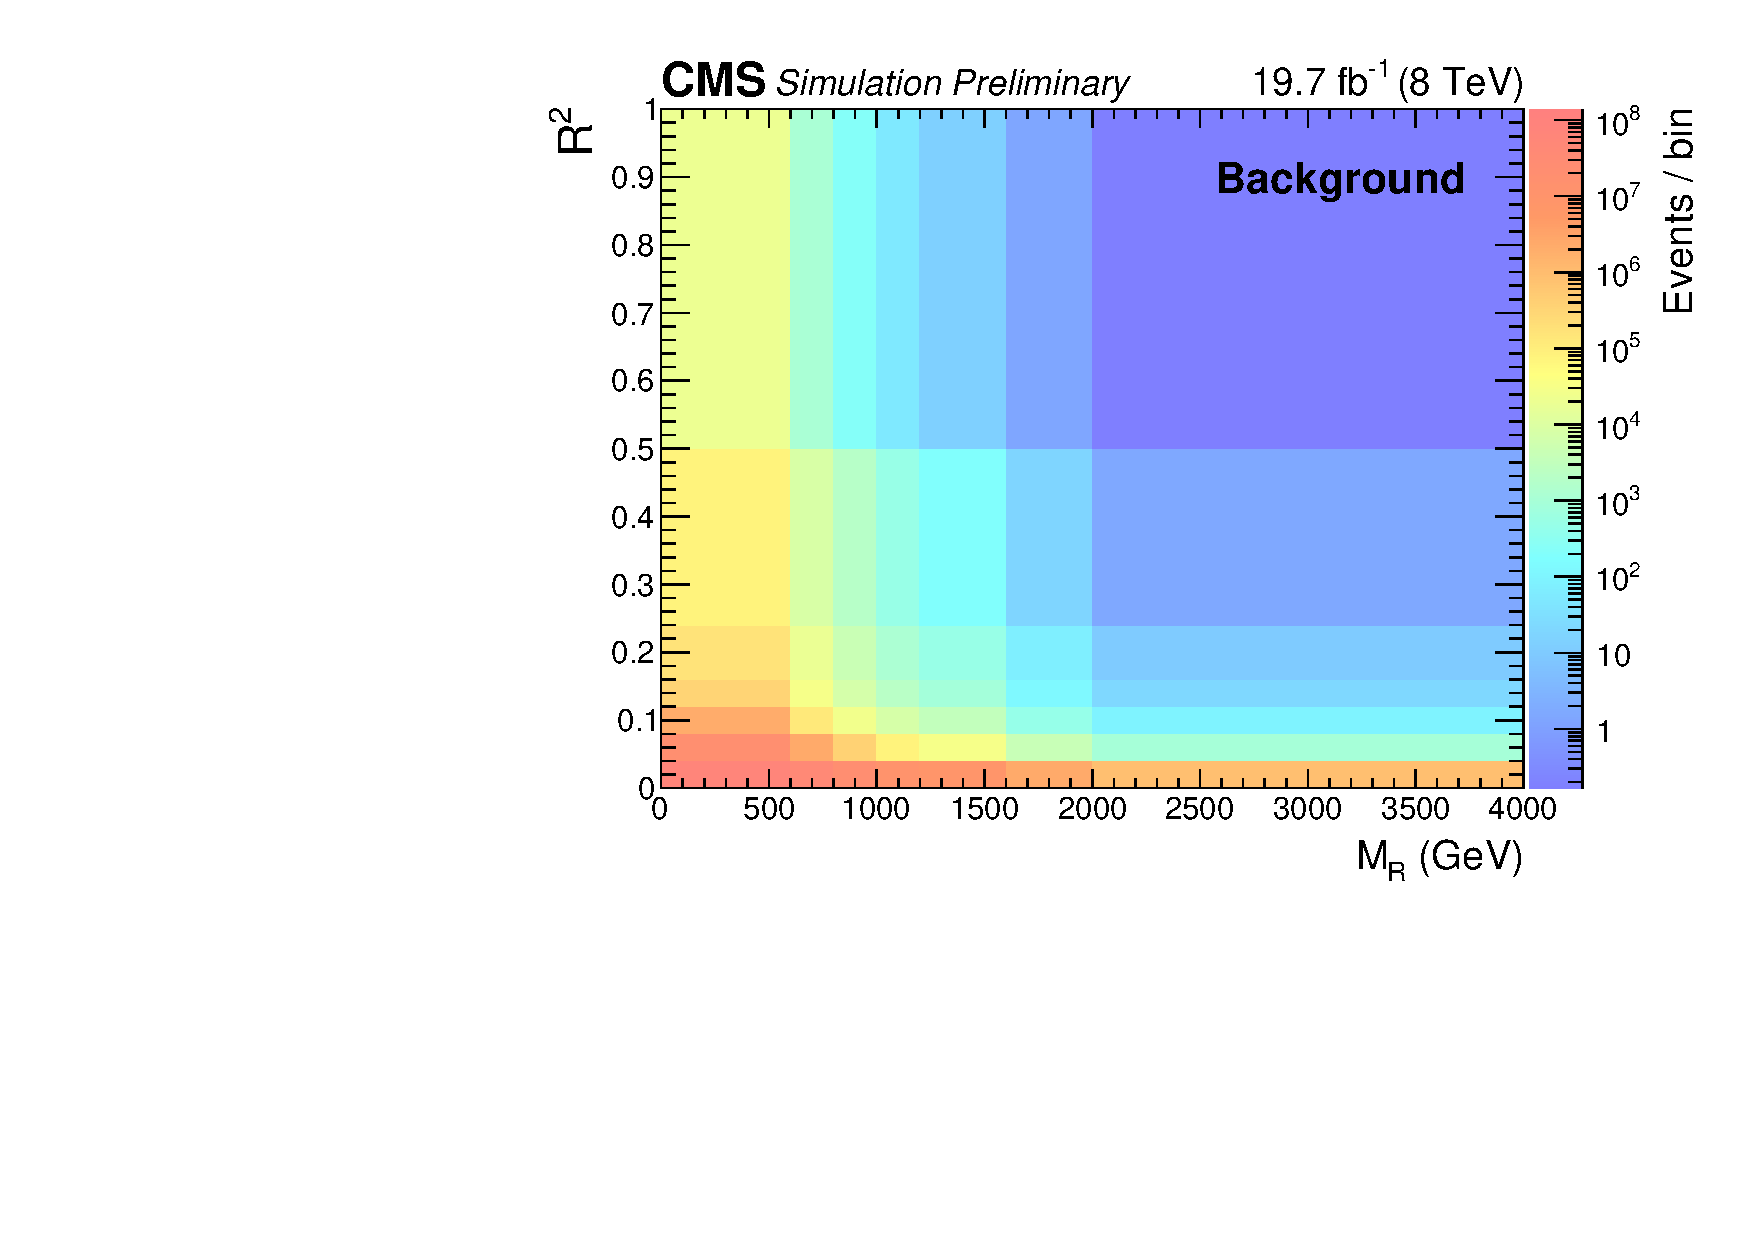
\includegraphics[width=0.49\textwidth]{figures/razor_variables/MR_R2_jet1ptg200_bg} 
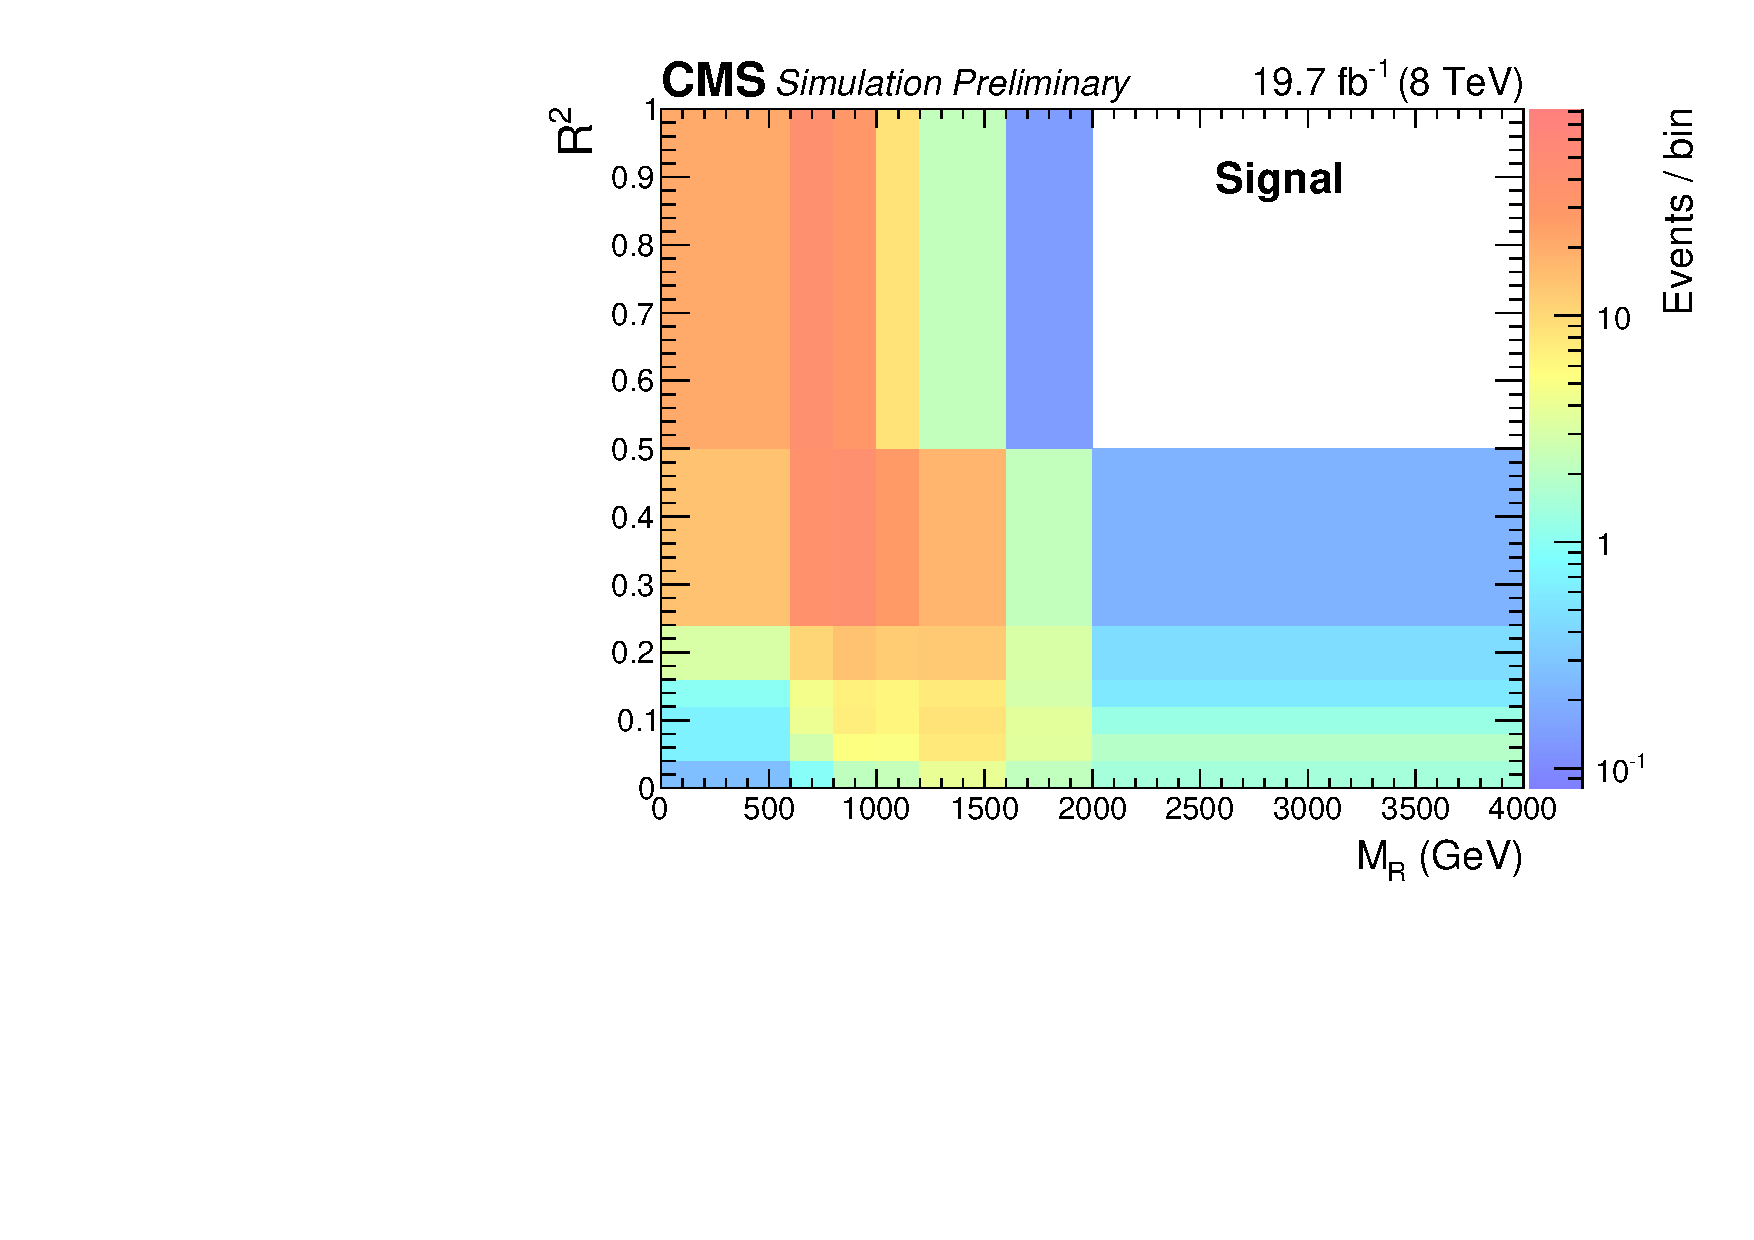
\includegraphics[width=0.49\textwidth]{figures/razor_variables/MR_R2_jet1ptg200_sig}
\caption{Distribution of the overall SM backgrounds and a T1ttcc signal with $m_{\tilde{g}} \,{=}\,
1\TeV$, $m_{\tilde{t}} \,{=}\, 325\GeV$ and $m_{\tilde{\chi}_1^0} \,{=}\, 300\GeV$, both obtained
from MC, on the (\mr,\rsq) space. A very loose selection is used:  a good primary vertex and at
least three jets, one of which should have $\pt > 200$ \GeV. 
\label{fig:razor_MR_Rsq_bg_signal}}

\end{figure}





\section[Boosted W boson tagging]{Boosted $\W$ boson tagging \label{sec:boost_wtag}}

%%%%%%%%%%%%%%%%%
% W tagging
%%%%%%%%%%%%%%%%%

One of the main highlights of the razor boost analysis is the tagging of boosted $\W$ bosons in
order to access a signal dominated phase space. 
$\W$ bosons either decay to two quarks, or to a lepton and a neutrino. The razor boost analysis is
an all-hadronic analysis, which means we do not explicitly consider the leptonic decays. 
$\W$ bosons with low to moderate transverse momentum will thus result in two jets, corresponding to
the two clusters of particles resulting from the hadronization of the two quarks. 
As the $\pt$ of the $\W$ boson increases, the separation between the two resulting jets decreases.
For high enough momentum, the two jets can no longer be fully resolved with the usual jet
definitions, and will be reconstructed as a single jet. This turnover in efficiency between the
resolved and merged case is illustrated in Fig.~\ref{fig:boost_wtag_ca8eff}.
Depending on the requirements on the jet multiplicity, losing a jet can result in a loss of signal
efficiency. We can, however, also use this effect to our advantage, namely to increase the
signal-to-background ratio by requiring the presence of one of these \textit{merged} jets. 
This, in turn, allows us to relax the jet multiplicity requirements. 

\begin{figure}
  \centering
  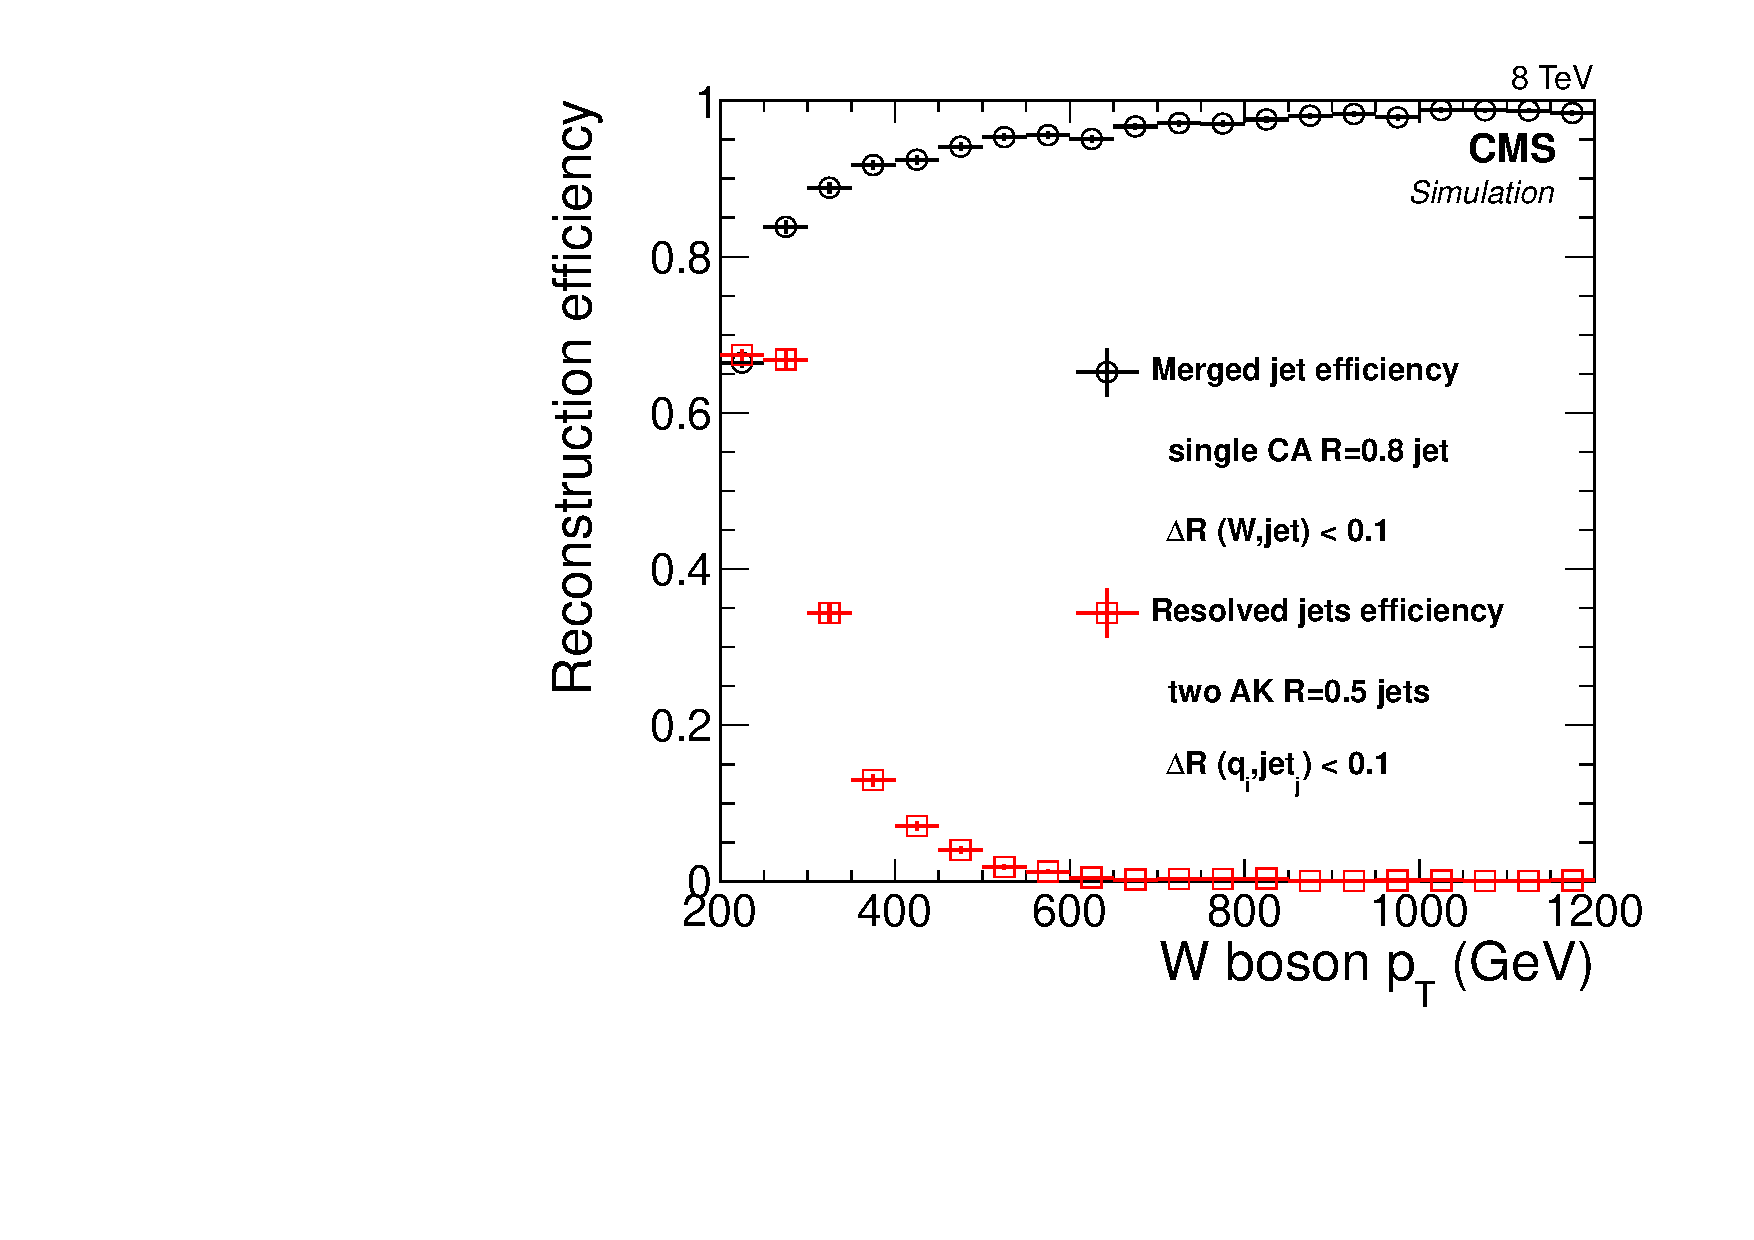
\includegraphics[width=0.8\textwidth]{figures/razor_wtag/ca8effVsPt}
  \caption{Efficiency to reconstruct a CA8 jet within $\Delta R<0.1$ of a generated $\W$ boson, and
the efficiency to reconstruct two AK5 jets within $\Delta R<0.1$ of the generated quarks from
longitudinally polarized $\W$ bosons, as a function of the $\pt$ of the $\W$
boson~\cite{Khachatryan:2014vla}. The loss in efficiency for the resolved case is clearly visible
for high $\pt$ $\W$ bosons. 
  \label{fig:boost_wtag_ca8eff}}
\end{figure}

The merged jet can be distinguished from other jets by its jet substructure, as illustrated in
Fig.~\ref{fig:boost_wtag_cartoon}. Jets originating from a $\W$ boson should have a two-prong
structure, whereas a quark/gluon-initiated jet is not expected to have this structure. 
In recent years, jet substructure techniques have seen very active developments, and many different
algorithms are on the market~\cite{Krohn:2009th,Gallicchio:2010sw,Butterworth:2008iy,Kaplan:2008ie}.
For the razor boost analysis we will use the CMS recommendation
in terms of which techniques to use~\cite{CMS-PAS-JME-13-006,Khachatryan:2014vla}. We will employ
\textit{jet pruning} and a set of variables called \textit{N-subjettiness}. On top of these jet
substructure techniques we will also use the jet mass variable to distinguish $\W$ boson-initiated
jets
from quark/gluon-initiated jets. 
The following subsections will go through the different parts of the
$\W$ tagging definition, providing a more detailed explanation for each.

\begin{figure}
  \centering
  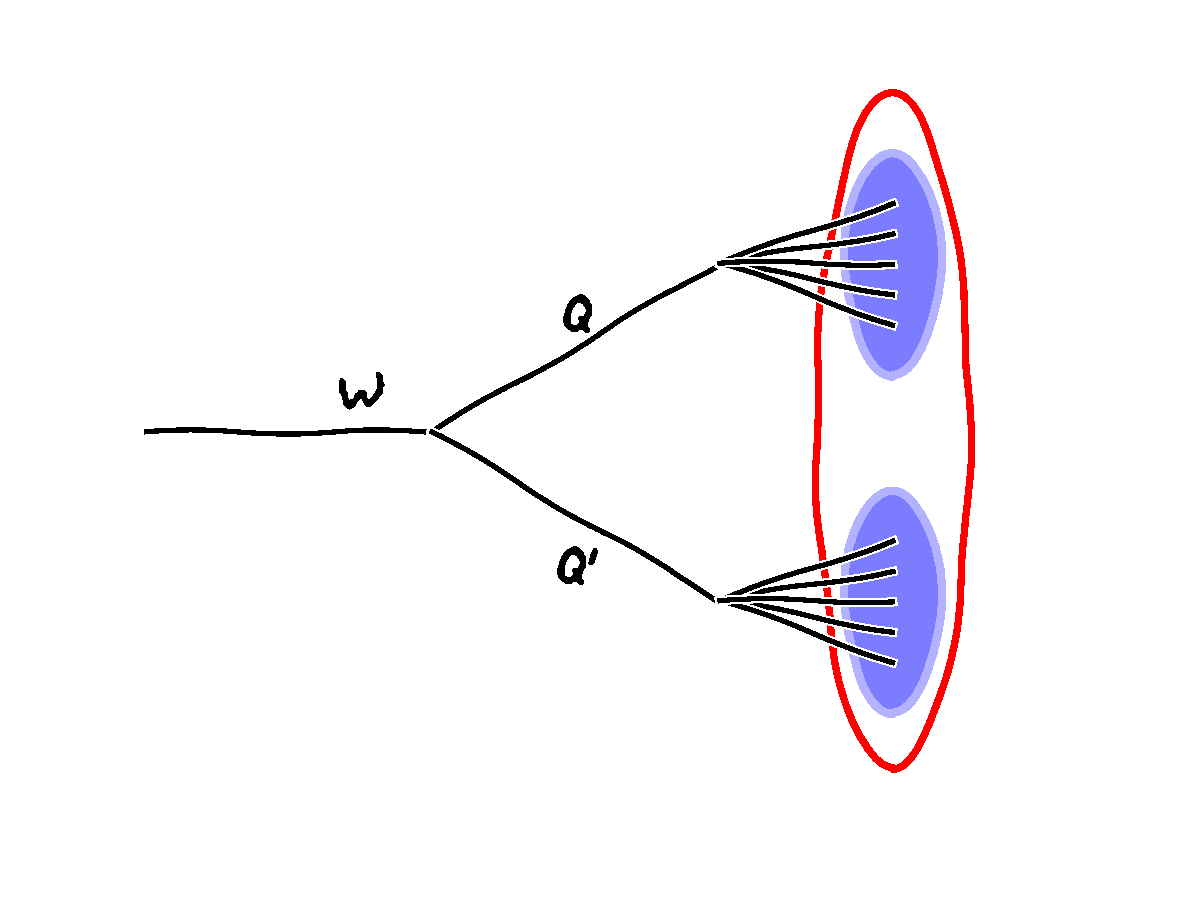
\includegraphics[width=0.48\textwidth]{figures/razor_wtag/W_subjets}
  ~
  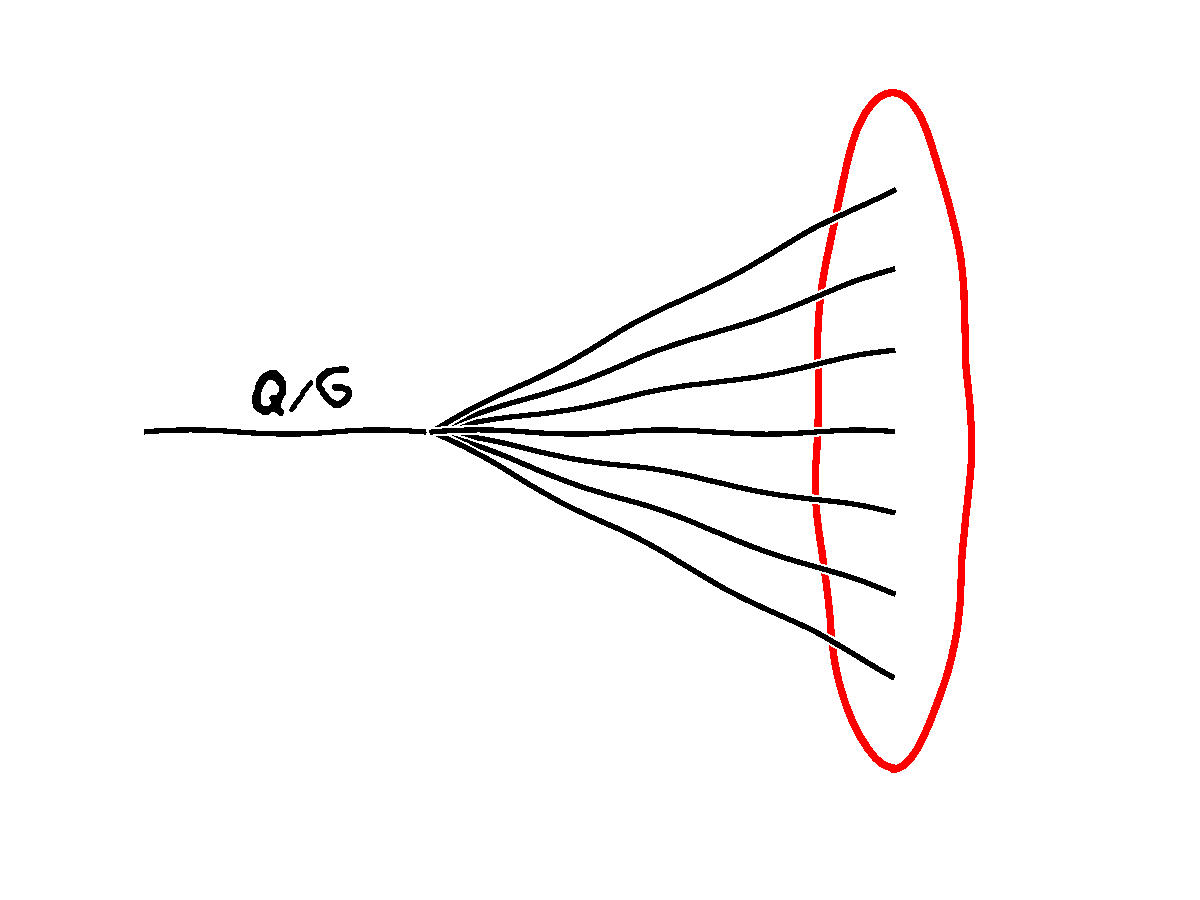
\includegraphics[width=0.48\textwidth]{figures/razor_wtag/qg_jets}
  \caption{The jet substructure of a $\W$-initiated jet differs from a quark/gluon-initiated jet.
  \label{fig:boost_wtag_cartoon}}
\end{figure}

%%%%%%%%%%%%%%%%%%%%%%%%%%%%%%%%%%%%%%%%%%%%%%%%%%%%%%%%%%%%%%%%%%%%%%%%%%%%%%%%%%%%%%%%%%%%%%%%%%%%

\subsection{Jet algorithm}

In order to identify boosted $\W$ bosons,  we will use a different jet clustering algorithm
than what is used for the standard jet definition (see Section~\ref{sec:object_jets}). 
Jets will be clustered with \textsc{FastJet 3.0.1.}~\cite{Cacciari:2011ma}, from the PF candidates,
using the Cambridge-Aachen (CA) algorithm~\cite{Dokshitzer:1997in} with a size parameter of 0.8.
Henceforth, we will call these jets \textit{CA8 jets}. 

%\begin{quote}
\begin{cajet} \theoremstyle{definition}
The Cambridge-Aachen jet algorithm is a sequential recombination algorithm that uses the
distance measure $d_{ij}$ between two constituents $i$ and $j$,
\begin{equation}
d_{ij} = \frac{\Delta R_{ij}^2}{R^2}, \label{eq:CA_distance}
\end{equation}
with $R$ the size parameter of the resulting jets, and
\begin{equation}
\Delta R_{ij}^2 = (y_i - y_j)^2 + (\phi_i - \phi_j)^2 ,
\label{eq:DeltaR_jet_algo}
\end{equation}
where $y, \phi$ are the rapidity (defined in Eq.~\ref{eq:rapidity}) and azimuthal angle. 
%The rapidity is given in terms of energy and longitudinal momentum as
%\begin{equation}
%  y = \frac{1}{2} \ln{\frac{ E + p_z }{ E - p_z }} .
%\end{equation}
The distance between constituent $i$ and the beam is given by $d_{iB} = 1$.
As is clear from the above, these distance measures only use angular information, unlike for the
$k_\mathrm{T}$ and anti-$k_\mathrm{T}$ algorithms, which use a $\pt$-weighted distance. 

The jet algorithm starts by computing the minimum distance $d_{ij}$, across all $i,j$. If $\min
d_{ij} < d_{iB}$, then we combine constituents $i$ and $j$ into a new constituent whose
four-momentum is the sum of the four-momenta of $i$ and $j$, and repeat the process. Otherwise, we
call $i$ a jet and move it from the list of constituents to be clustered to the list of final jets.
The process is repeated with the remaining constituents, until none remain.
\end{cajet}


Jet energy corrections for these CA8 jets are derived from the standard anti-$k_\textrm{T}$ jets
with size parameter $R=0.7$. Simulations show that the corrections are valid for CA8 jets and
have an additional uncertainty no greater than 2\%~\cite{CMS-PAS-JME-13-007,CMS-AN2012-393}.  
% seems like no better reference is available for this...

%%%%%%%%%%%%%%%%%%%%%%%%%%%%%%%%%%%%%%%%%%%%%%%%%%%%%%%%%%%%%%%%%%%%%%%%%%%%%%%%%%%%%%%%%%%%%%%%%%%%

\subsection{Jet pruning}

Jet pruning~\cite{Ellis:2009su,Ellis:2009me} is a particular kind of jet grooming. Jet grooming
techniques are designed to reduce the impact of contributions from the underlying event (UE), pileup
(PU), and low-\pt gluon radiation. These kinds of contributions to jets are typically soft and
diffuse, and increase the jet energy proportional to the jet area. Grooming techniques reduce the
jet area without affecting the core components. This means that the resulting jets are less
sensitive to these soft contributions, but still reflect the kinematics of the original, hard
process.


During jet pruning the constituents of the jet are reclustered with the CA algorithm, using the
same distance parameter as used for the original jets (here $R=0.8$), but with additional conditions
beyond those of the standard algorithm.
In particular, the softer and larger-angle of the two particles $i$ and $j$ to be merged is removed
when the following conditions are satisfied:
\begin{align}
  z_{ij} &= \frac{\min( \pt^i , \pt^j )}{\pt^i + \pt^j} < z_{\textrm{cut}}, \\
  \Delta R_{ij} &> D_{\textrm{cut}} \equiv \alpha \frac{m_J}{\pt} ,
\end{align}
where $m_J$ and $\pt$ are the original mass and transverse momentum of the reclustered jet,
$\Delta R_{ij}$ is defined as in Eq.~\ref{eq:DeltaR_jet_algo}, and
$z_\textrm{cut}$ and $\alpha$ are parameters of the algorithm, chosen to be 0.1 and 0.5,
respectively~\cite{Chatrchyan:2013vbb}. 

The resulting pruned jet is used as further input to our $\W$ boson tagger. For the $\W$ decay
products to be collimated, we need a large transverse momentum. We will therefore require that the
pruned jets have $\pt > 200\GeV$. 
Because of the reduction of the effect of UE and PU, the jet mass variable as computed from the
constituents of the jet after jet pruning has a much better behaviour than if it was computed from
the unpruned jets, as seen on Fig.~\ref{fig:wtag_jet_pruning}. Jet pruning shifts the jet mass of
QCD jets
to smaller values, while maintaining the jet mass for $\W$ jets close to the $\W$ boson mass.

We will make the requirement that the pruned jet mass is consistent with the $\W$ boson mass,
\begin{equation}
  70 < m_{\textrm{pruned jet}} < 100 \GeV .
\end{equation}
Here, we have deviated from the standard interval used in CMS, starting at 60\GeV, as we found that
for our
kinematical region and signal topology we achieve better signal to background discrimination when
increasing the lower cut value to 70\GeV. 
%This provides good boosted $\W$ jet to quark/gluon jet discrimination. 

\begin{figure}
  \centering
  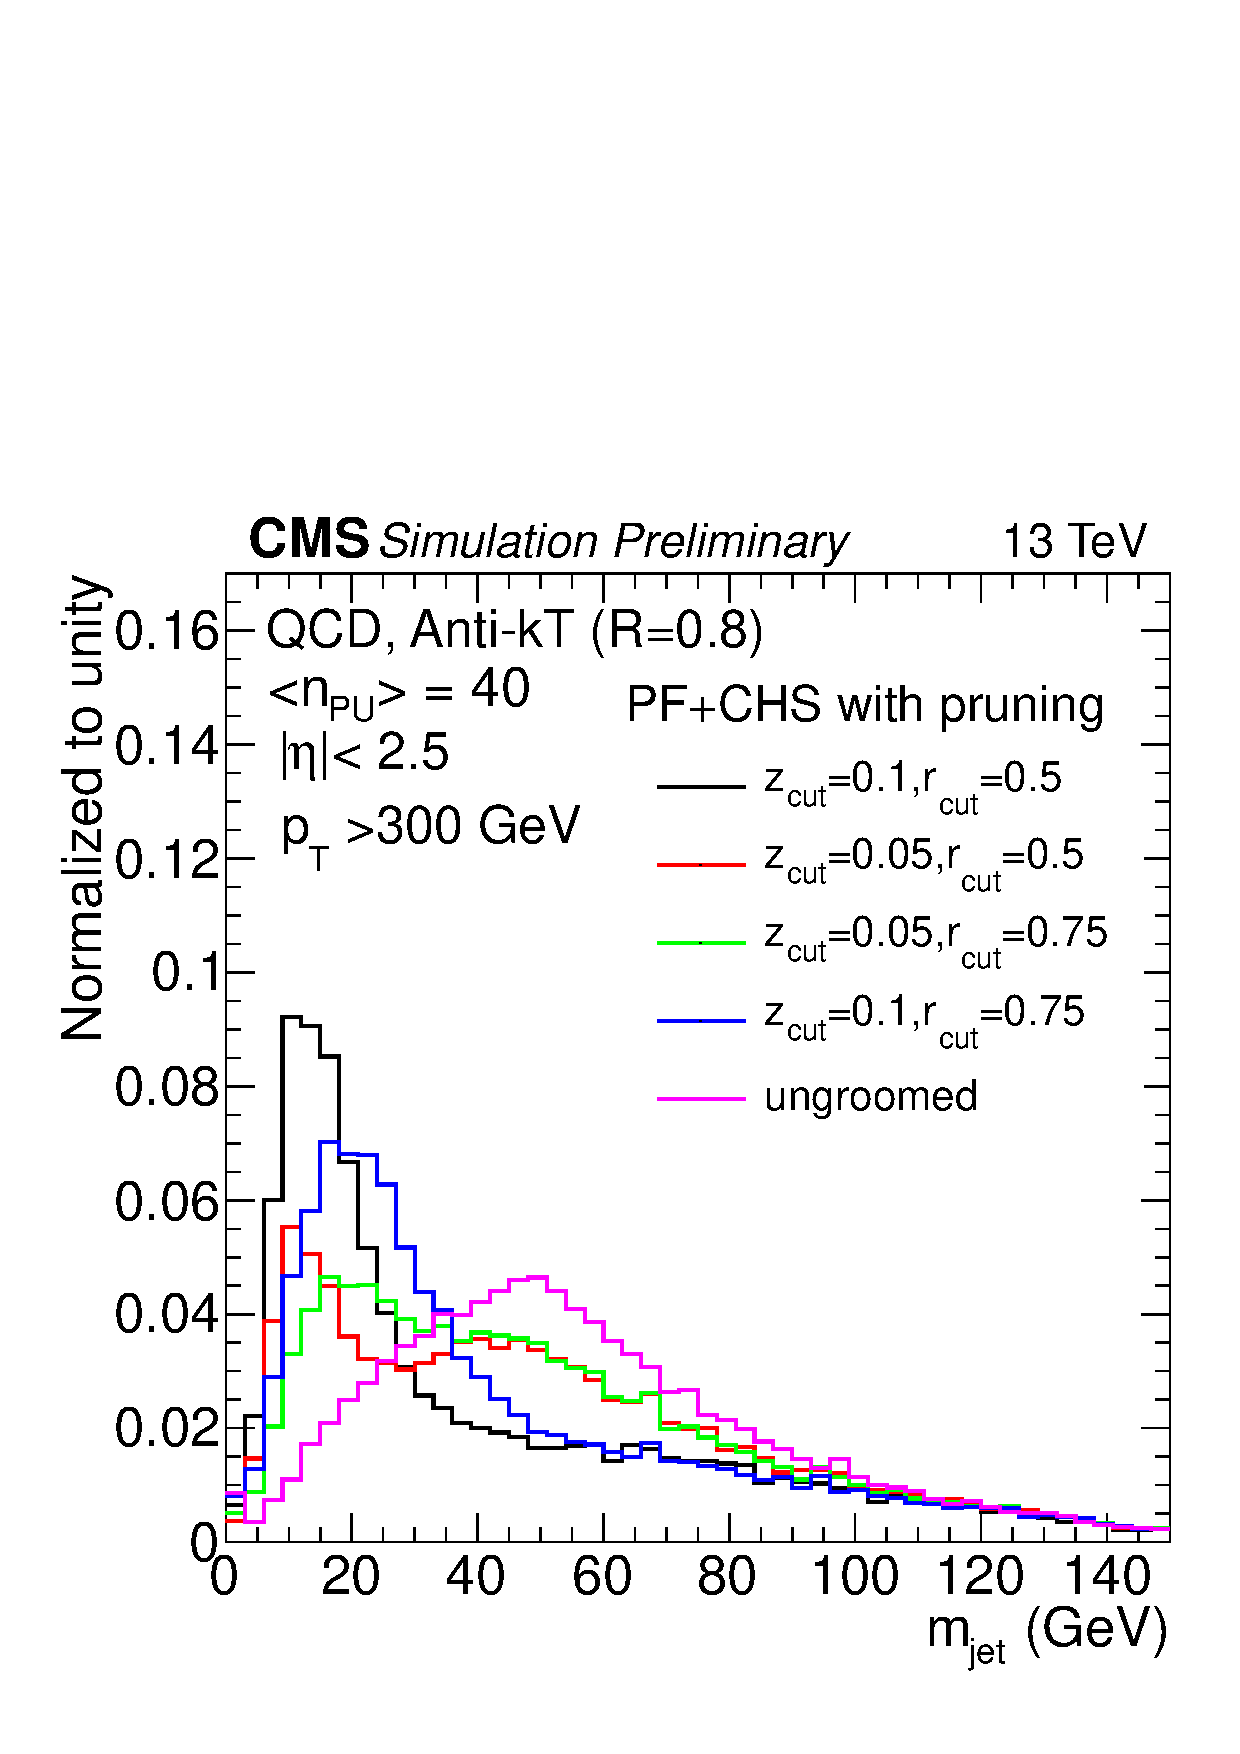
\includegraphics[width=0.6\textwidth]{figures/razor_wtag/1DPFCHS_PR_QCD}
  \caption{Jet mass distribution of QCD jets with $\pt(\textrm{gen}) > 300 \GeV$ for jet pruning
with different parameters, starting from PF jets with charged-hadron subtraction applied. The fully
ungroomed mass distribution is also shown for comparison. Here, the jets were clustered using the
anti-$k_\mathrm{T}$ algorithm, but the same picture holds for Cambridge-Aachen jets.
Figure taken from~Ref.\cite{CMS-PAS-JME-14-001}. 
  \label{fig:wtag_jet_pruning}}
\end{figure}

%%%%%%%%%%%%%%%%%%%%%%%%%%%%%%%%%%%%%%%%%%%%%%%%%%%%%%%%%%%%%%%%%%%%%%%%%%%%%%%%%%%%%%%%%%%%%%%%%%%%

\subsection{N-subjettiness}

Requiring the jet mass to be consistent with the $\W$ boson mass already results in a good
discrimination between $\W$ boson and quark/gluon-initiated jets. We can, however, still do better.
A boosted QCD jet with a mass around 80\GeV usually originates from a single hard parton and
acquires mass through large-angle soft splittings. The energy pattern for this process will differ
from the two-prong pattern that is found in boosted $\W$ jets.  
The set of N-subjettiness observables $\tau_N$~\cite{Thaler:2010tr} aims to exploit this difference
in expected energy flow to differentiate between $\W$ boson and quark/gluon-initiated jets by
counting the number of hard lobes of energy within a jet.

N-subjettiness is computed under the assumption that the jet has N subjets, and is the
$\pt$-weighted $\Delta R$ distance between each jet constituent and its nearest subjet axis:
\begin{equation}
\tau_N = \frac{1}{R_0 \sum_{k} p_{T, k}} \sum_k p_{T, k} \min (\Delta R_{1,k}, \Delta R_{2,k}, ...
\Delta R_{N,k}),
\end{equation}
where $R_0$ is the original jet distance parameter (0.8 in our case) and $k$ runs over all
constituent particles of the jet. 
The subjet axes are obtained by running the exclusive $k_T$
algorithm~\cite{Ellis:1993tq,Catani:1993hr} using \textsc{FastJet}. 
The exclusive $k_T$ algorithm differs from the inclusive version in two ways: if at a given
clustering step $d_{iB} < \min_j d_{ij}$, then constituent $i$ is discarded, rather than added to
the jet collection; and the clustering stops when the desired number of jets (N) is reached. 
The resulting axes can be further optimized to minimize the N-subjettiness value. In accordance to
the CMS recommendation, we use a “one-pass” optimization of the exclusive $k_T$
axes~\cite{nsubjettiness_fastjet}.

The variables $\tau_N$ quantify the consistency of the jet having N or fewer subjets. They have a
small value (close to 0) if the original jet is consistent with having N or fewer subjets, because
almost every jet constituent will be close in $\Delta R$ to its own true subjet. 
As we are interested in discriminating boosted $\W$ bosons, with two subjets, from quark/gluon
jets, which have a single subjet, we will use the variables $\tau_2$ and $\tau_1$, as obtained
from the unpruned CA8 jets.   
It has been shown that the ratio of the $\tau_N$ variables are better discriminators than the
separate variables~\cite{Thaler:2010tr}. We will thus require that the ratio $\tau_2 / \tau_1$ is
small. 
To ensure that the N-subjettiness ratio as computed from the unpruned
jet collection is assigned to the correct pruned jet, we find the highest \pt unpruned jet that is
within $\Delta R = 0.7$ of the considered pruned jet.
The $\tau_2 / \tau_1$ distribution for highly boosted and longitudinally polarized $\W$
bosons and for inclusive QCD jets is shown in Fig.~\ref{fig:boost_wtag_tau2tau1}. 

\begin{figure}[htb]
  \centering
  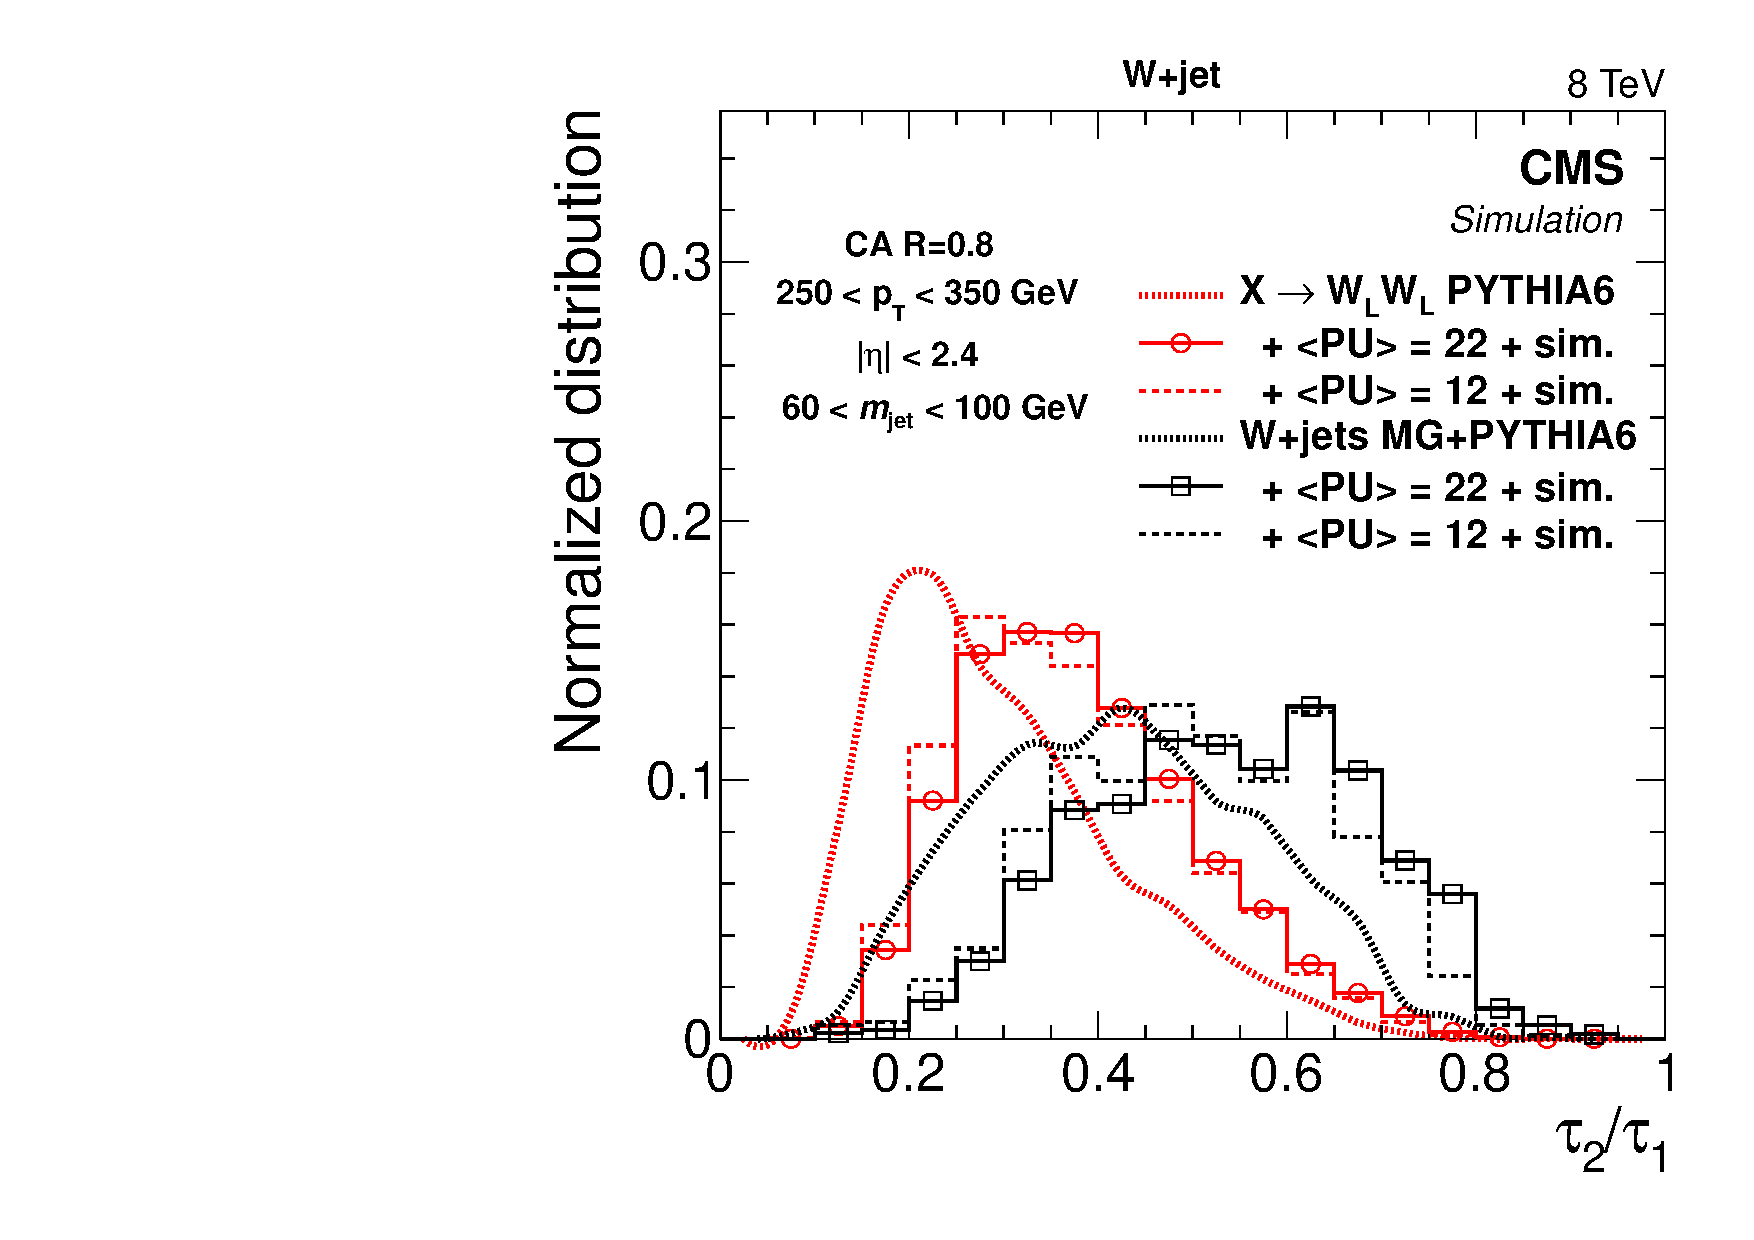
\includegraphics[width=0.8\textwidth]{figures/razor_wtag/tau2tau1_afterMass}
  \caption{Distributions of the N-subjettiness ratio $\tau_2 / \tau_1$ in simulated samples of
highly boosted and longitudinally polarized $\W$ bosons and inclusive QCD jets expected in the
$\W$+jet topology (\ie with leptonically decaying $\W$ bosons recoiling off a hard jet). 
The distribution is shown after a selection on the pruned jet mass of $60 < m_{\textrm{pruned jet}}
< 100 \GeV$. Note that this is slightly different from what is applied in the razor boost analysis.
Thick dashed lines represent the generator predictions without pileup interactions and without CMS
detector simulation. The histograms are the expected distributions after full CMS simulation with
pileup corresponding to an average number of 12 and 22 interactions~\cite{Khachatryan:2014vla}. 
  \label{fig:boost_wtag_tau2tau1}}
\end{figure}


%%%%%%%%%%%%%%%%%%%%%%%%%%%%%%%%%%%%%%%%%%%%%%%%%%%%%%%%%%%%%%%%%%%%%%%%%%%%%%%%%%%%%%%%%%%%%%%%%%%%

\subsection{\texorpdfstring{$\W$}{W} boson tagging definitions}

In the razor boost analysis we will employ a boosted $\W$ boson tagger, utilizing the techniques
outlined in the previous sections, to identify events that are consistent with the presence of a
high \pt, hadronically decaying $\W$ boson. 
A given pruned CA8 jet is $\W$ tagged if it has $\pt > 200\GeV$, $|\eta|<2.4$, $70 < m_\textrm{jet}
< 100\GeV$, and the corresponding unpruned jet satisfies $\tau_2 / \tau_1 < 0.5$.
This definition is the same as was used previously in a search for massive resonances in dijet
systems containing jets tagged as a W or Z boson~\cite{EXO-12-024,EXO-13-009}. 
The precise definition of this $\W$ boson tagger is summarized in Table~\ref{tab:Wtag_definition}.

As explained in Section~\ref{sec:boost_strategy}, we will use three control regions to select data
samples enriched in QCD multijet, $t\bar{t}$, and $\W(\rightarrow l \nu)+$jets, in order to help
model the SM backgrounds. QCD multijet and leptonically decaying $\W$+jets events are not expected
to have jets with a two-prong substructure. Therefore, our $\W$ boson tagging definition will not be
very efficient in selecting these processes. To remedy this, we slightly modify our $\W$ tagger. 
We define $\W$ boson \textit{anti-tagged} jets (aW) by taking the complement of the $\tau_2 /
\tau_1$ requirement, and define $\W$ boson \textit{mass-tagged} jets (mW) by dropping that
requirement all together. 
These definitions allow a more efficient selection of background processes, while remaining in a
similar kinematic regime. How these taggers will be used exactly will be explained in
Section~\ref{sec:boost_control_selection} when discussing the event selection. A summary of their
definitions can be found in Table~\ref{tab:Wtag_definition} as well. 

\begin{table}[htdp]
\caption{Boosted $\W$ tagging definitions. The input jet collection is either the pruned or unpruned
CA8 jet collection with charged-hadron subtraction applied. }
\vspace{1ex}
\centering
\begin{tabular}{l c c c}
\toprule
& $\W$ & aW & mW  \\
\midrule
\multirow{3}{*}{Pruned} & $\pt > 200$  & $\pt > 200$  & $\pt > 200$\\
& $|\eta| < 2.4$ & $|\eta| < 2.4$ & $|\eta| < 2.4$\\
& $70 < m_{\textrm{jet}}< 100$ & $70 < m_{\textrm{jet}}< 100$ & $70 < m_{\textrm{jet}}< 100$\\
\midrule
Unpruned & $\tau_2 / \tau_1 < 0.5$ & $\tau_2 / \tau_1 \geq 0.5$ & -\\
\bottomrule
\end{tabular}
\label{tab:Wtag_definition}
\end{table}

%%%%%%%%%%%%%%%%%%%%%%%%%%%%%%%%%%%%%%%%%%%%%%%%%%%%%%%%%%%%%%%%%%%%%%%%%%%

\subsection{\texorpdfstring{$\W$}{W} boson tagging scale factors \label{sec:wtag_scale_factor}}

It has been observed by previous CMS analyses that the $\W$ boson tagging efficiency is not the same
in data and in simulation. The distributions that are at the root of this disagreement are shown on
Fig.~\ref{fig:boost_wtag_data_sim}. 
To account for the discrepancies, we need to derive data/MC scale factors and associated
uncertainties corresponding to each of the $\W$ boson tagging, mass-tagging and anti-tagging
definitions listed in Table~\ref{tab:Wtag_definition}. These scale factors are not
process-independent. They will be different for processes that include hadronically decaying $\W$
bosons, such as $t\bar{t}$ or the signal, compared to processes which do not have $\W$ bosons in
their final state, such as QCD multijet production. For processes without real hadronically
decaying $\W$ bosons, any tagged jet is necessarily a misidentified, or \textit{fake}, $\W$ boson
tag. For those processes we will speak of the $\W$ boson tagging fake rate scale factors, where the
fake rate is defined as the probability to tag, with one of the used $\W$ tagging definitions, a jet
not coming from a hadronically decaying $\W$ boson. 
One last consideration concerns the signal simulation. As the signal is simulated with FastSim, we
need an additional scale factor to correct for differences in the modelling of the $\W$ tagger
between FastSim and FullSim. 
In the following subsections every scale factor will be listed in more detail, including how it was
derived and how it will be used in the analysis. 

\begin{figure}[htpb]
  \centering
  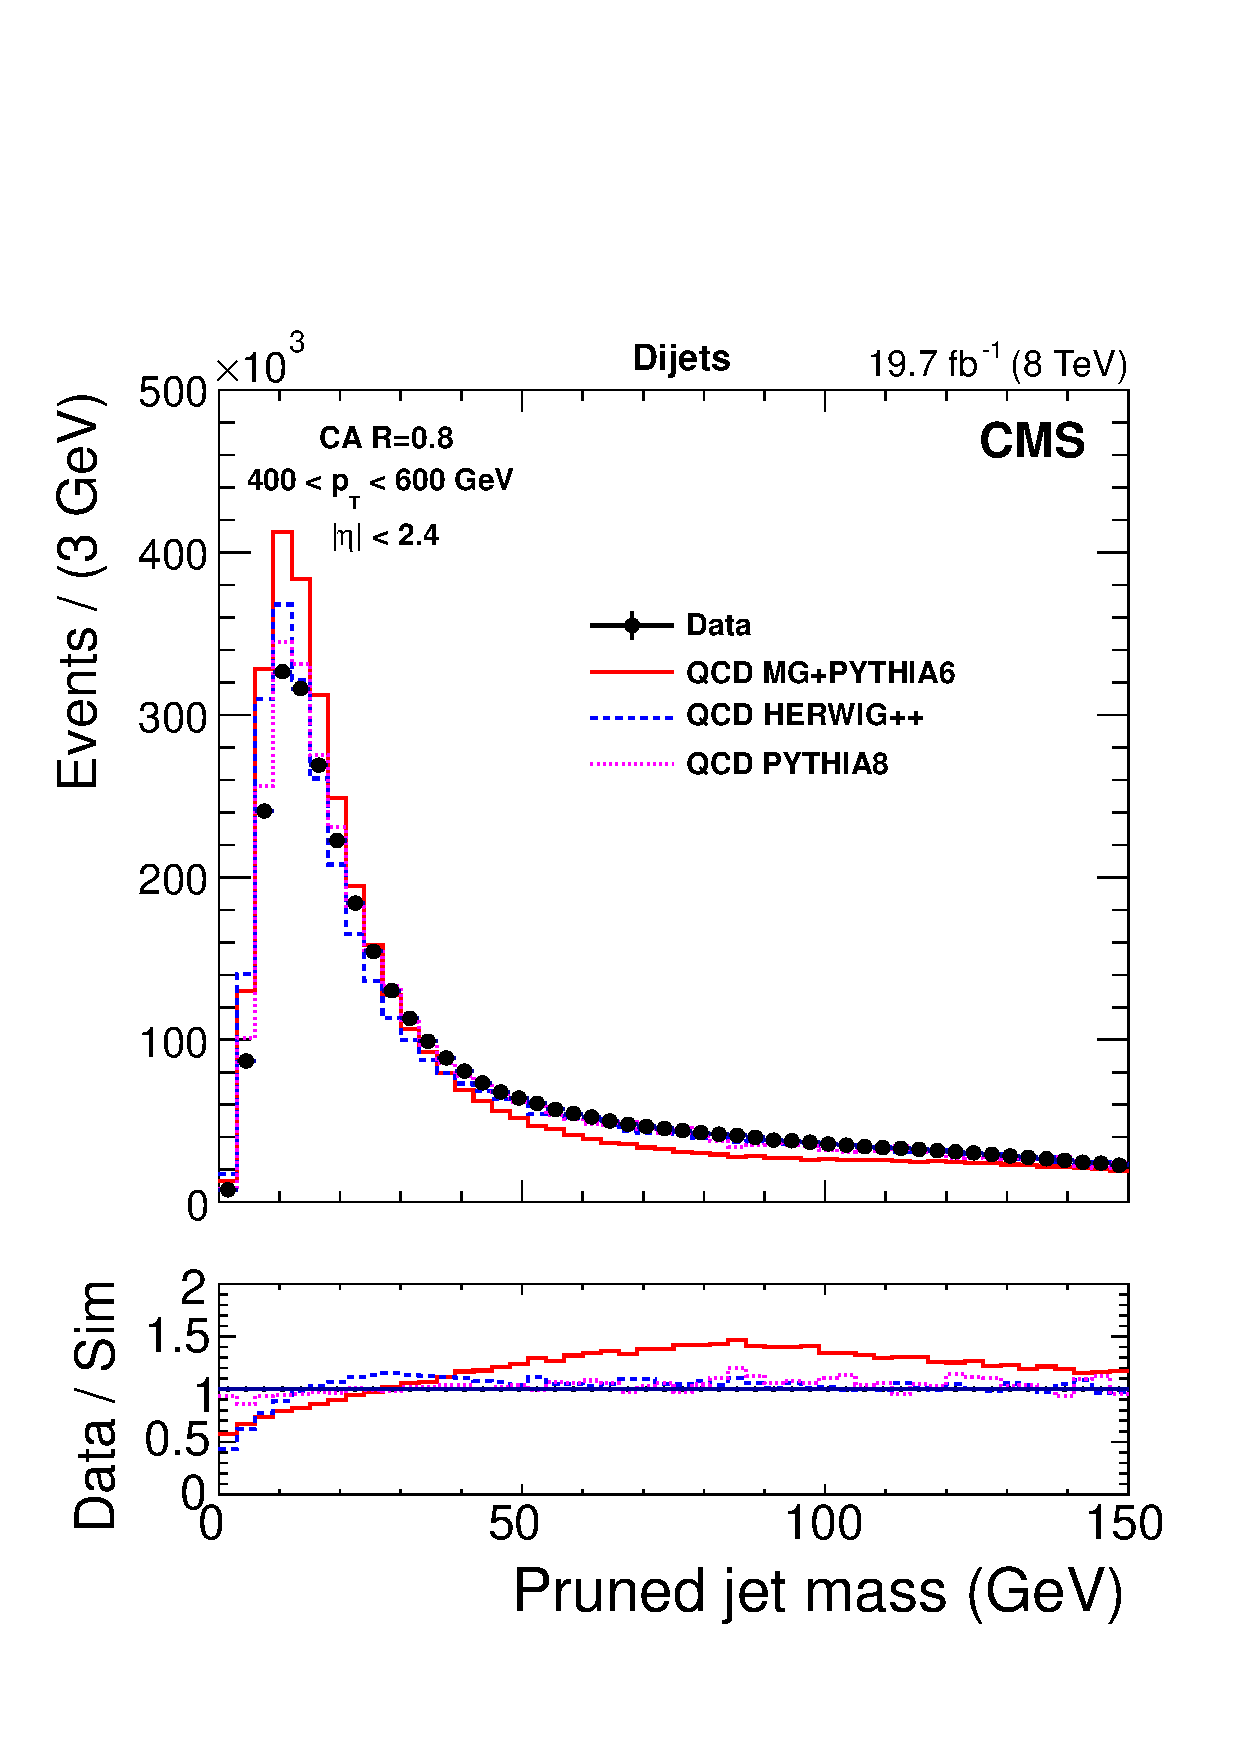
\includegraphics[width=0.48\textwidth]{figures/razor_wtag/substructure_pas_mass_2}
  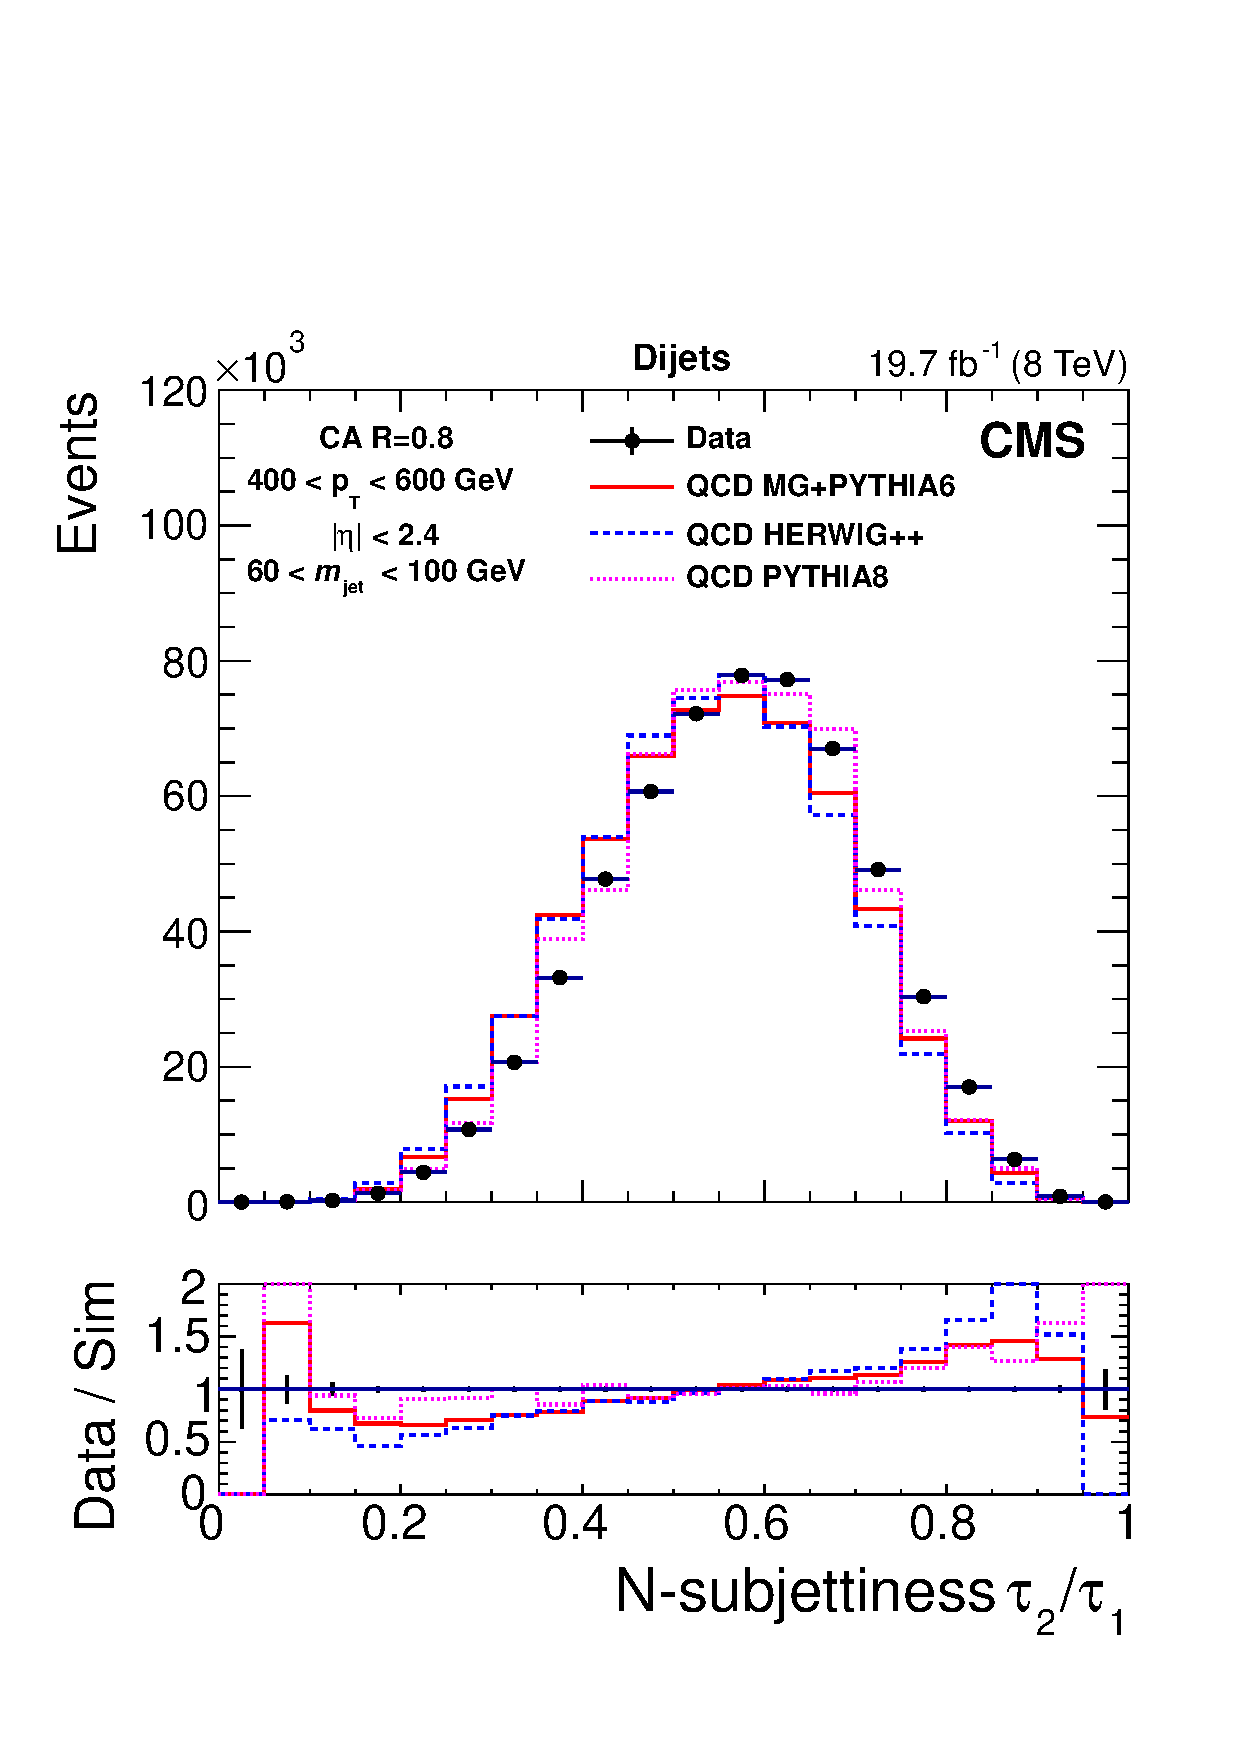
\includegraphics[width=0.48\textwidth]{figures/razor_wtag/substructure_pas_tau21_aftermass_2}
  \caption{Pruned jet mass (left) and N-subjettiness ratio $\tau_2/\tau_1$ (right) distributions 
  in data and simulation for dijet events. MG denotes the \MADGRAPH generator, and is the option
used for the razor boost analysis. The relative deviations between
data and simulation are plotted at the bottom of each figure~\cite{Khachatryan:2014vla}. 
  \label{fig:boost_wtag_data_sim}}  
\end{figure}

%% ---------------------------------------------------------------------------------------------

\subsubsection{\texorpdfstring{$\W$}{W} boson tag efficiency scale factor \label{sec:wtag_eff_sf}}

The $\W$ boson tag efficiency scale factor will be used to correct processes with real
hadronically decaying $\W$ bosons. For the backgrounds this is mainly for the $t\bar{t}$ process,
but also single top and $t\bar{t}$ in association with a $\W$ or $\cPZ$ boson are considered. This
scale factor is of course also used for the signal processes. 

The $\W$ boson tag efficiency scale factor is only applied to the simulation in the $S$ and $T$
region, see Sections~\ref{sec:boost_signal_selection} and \ref{sec:boost_T_region}, as those are the
regions that utilize the $\W$ tagging definition in their selection criteria. It is also only
applied to events for which the $\W$ boson tagged jet is matched (within a cone of $\Delta R = 0.8$)
to a generator level hadronically decaying $\W$ boson. In case no match was found, we apply the $\W$
boson tag fake rate scale factor. 

As we use the same $\W$ boson tagging definition as was used in a search for massive resonances in
dijet systems containing $\W$ tagged jets~\cite{EXO-12-024}, we can directly apply the scale
factor that was derived for that study. The
method used to obtain the scale factor is outlined in Ref.~\cite{CMS-PAS-JME-13-006}. 
The $\W$ boson tag efficiency scale factor $SF_{\textrm{Wtag}}$ is given by
\begin{equation}
SF_{\textrm{Wtag}} = 0.86 \pm 0.07 .
\end{equation}


%% ---------------------------------------------------------------------------------------------

\subsubsection{\texorpdfstring{$\W$}{W} boson tag efficiency FullSim/FastSim scale factor
\label{sec:wtag_eff_fastfull_sf}}

For our signal samples, which are produced with FastSim, we have derived an additional $\W$ tag
efficiency FullSim/FastSim scale factor, $SF_{\textrm{Full/Fast}}$, which depends on the \pt
of the CA8 jet. This scale factor corrects for the different modelling of jets, jet
substructure, etcetera, in FastSim with respect to FullSim. The product of $SF_{\textrm{Wtag}}$ and
$SF_{\textrm{Full/Fast}}$ will be applied to the signal simulation. 

To compute the $\W$ boson tag efficiency FullSim/FastSim scale factor we use a sample of $t\bar{t}$
events simulated with both FullSim and FastSim. 
A FastSim versus FullSim comparison of the distributions of the pruned jet mass, the N-subjettiness
variables $\tau_1$, $\tau_2$ and their ratio $\tau_2/\tau_1$, both before and after requiring the
jets to satisfy the pruned jet mass window, is shown in
Figs.~\ref{fig:FastFull_jmass}--\ref{fig:FastFull_tau21}. It is clear that the agreement is not
perfect. The $\tau_2/\tau_1$ distribution for FastSim is shifted with respect to FullSim. This
disagreement will then of course be translated into the efficiencies, and thus the need for a scale
factor arises. 

\begin{figure}[htpb]
\centering
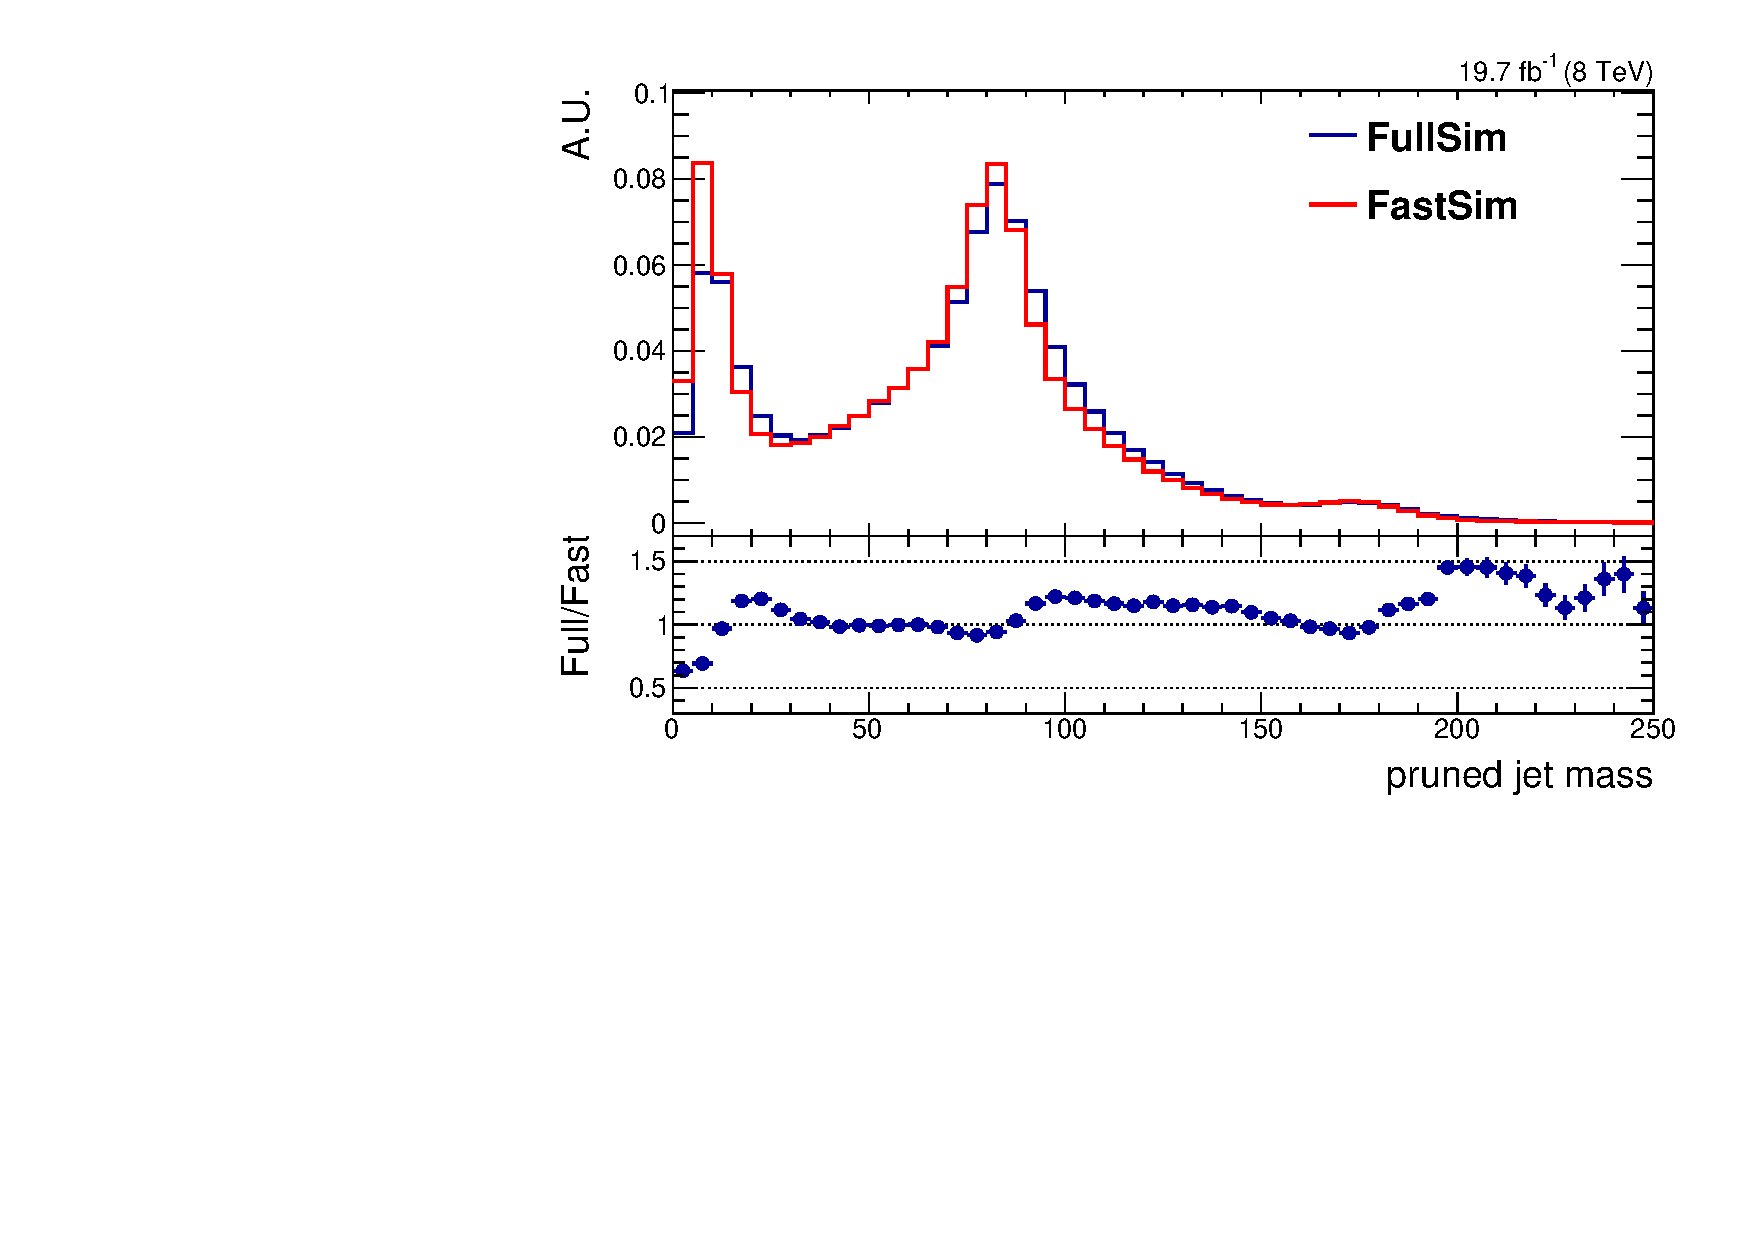
\includegraphics[width=0.7\textwidth]{figures/razor_wtag/FastFull_comparison_TTJets_jmass}
\caption{Pruned jet mass distribution for FastSim and FullSim $t\bar{t}$. 
\label{fig:FastFull_jmass}}
\end{figure}

\begin{figure}[p]
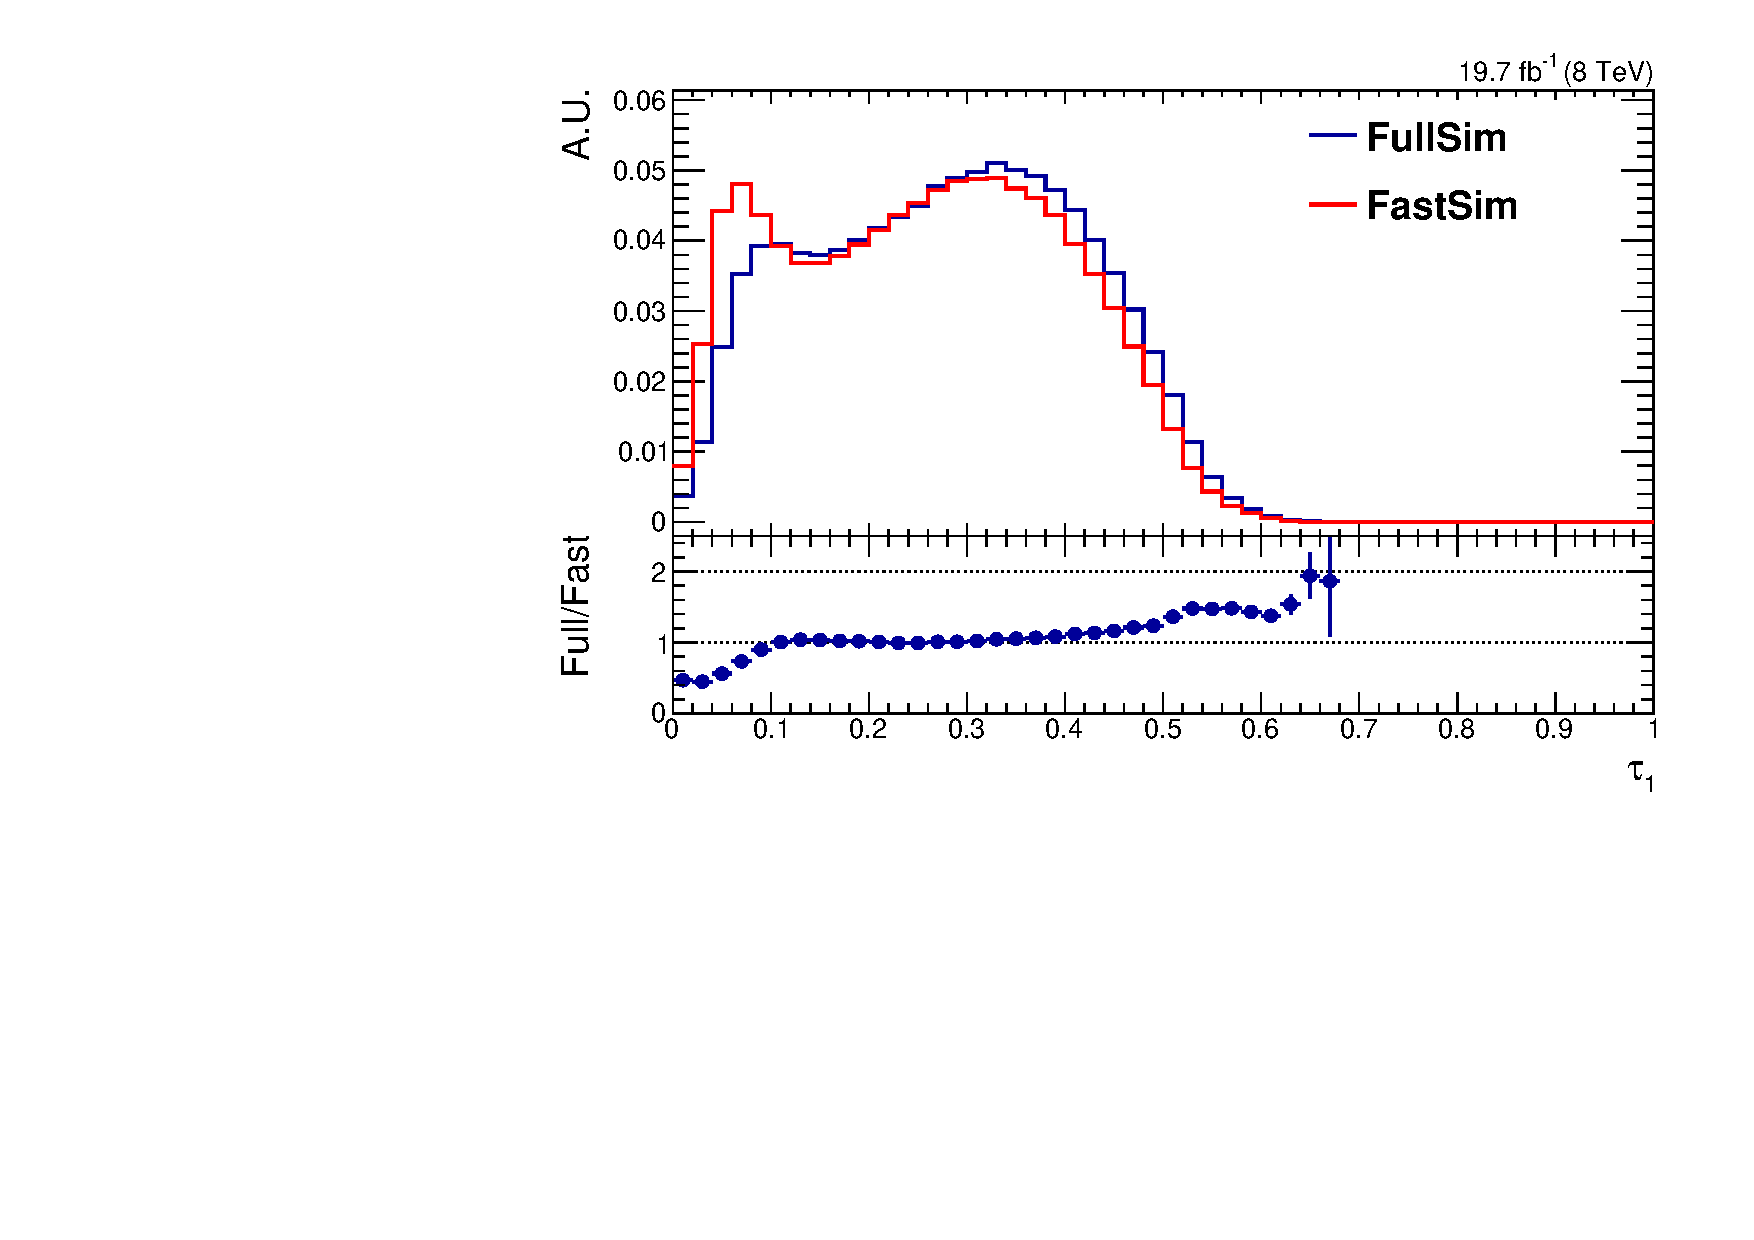
\includegraphics[width=0.49\textwidth]{figures/razor_wtag/FastFull_comparison_TTJets_tau1}
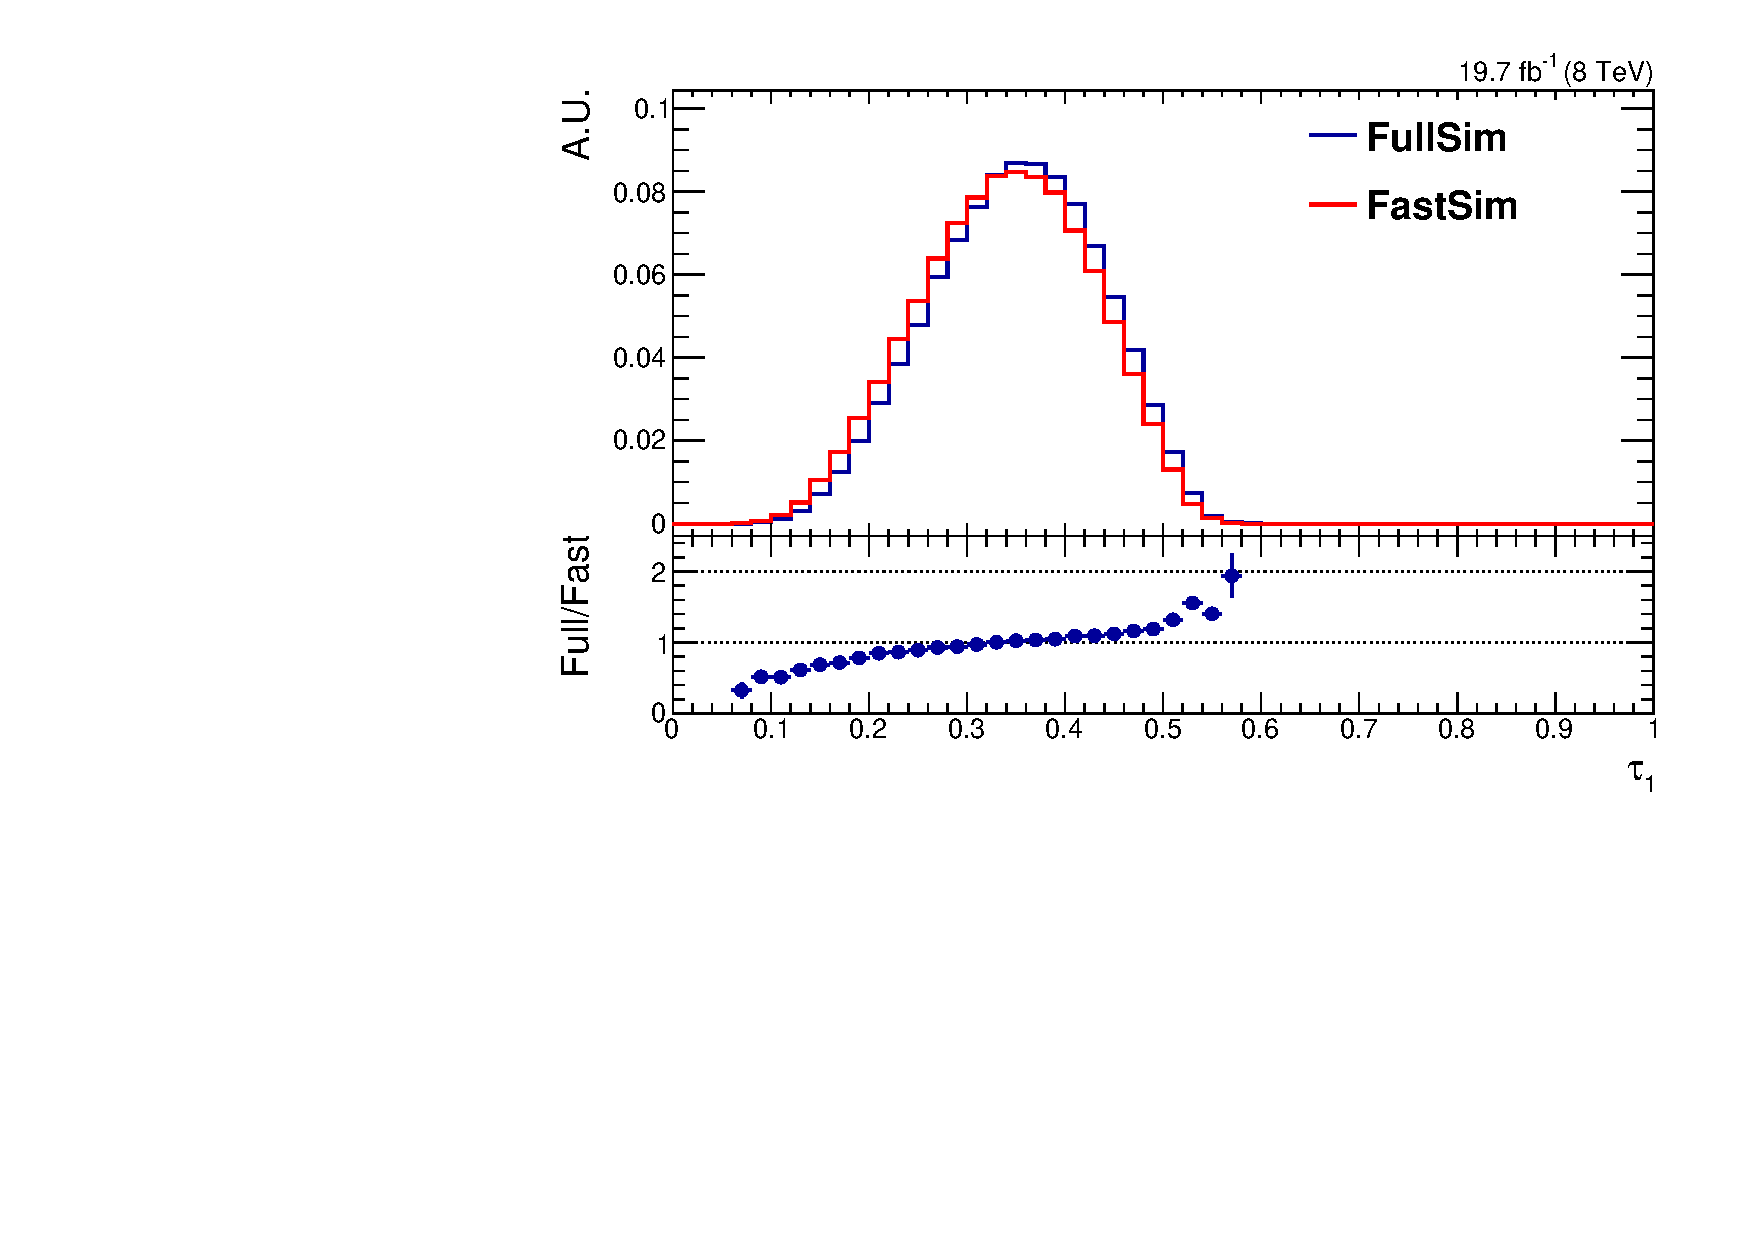
\includegraphics[width=0.49\textwidth]{figures/razor_wtag/FastFull_comparison_TTJets_tau1_masscut}
\caption{Distribution of $\tau_1$ before (left) and after (right) requiring the pruned CA8 jet to
lie within the $\W$ mass window, $70 < m_{\textrm{jet}} < 100$\GeV, for FastSim and
FullSim $t\bar{t}$.
\label{fig:FastFull_tau1}}
\end{figure}

\begin{figure}[p]
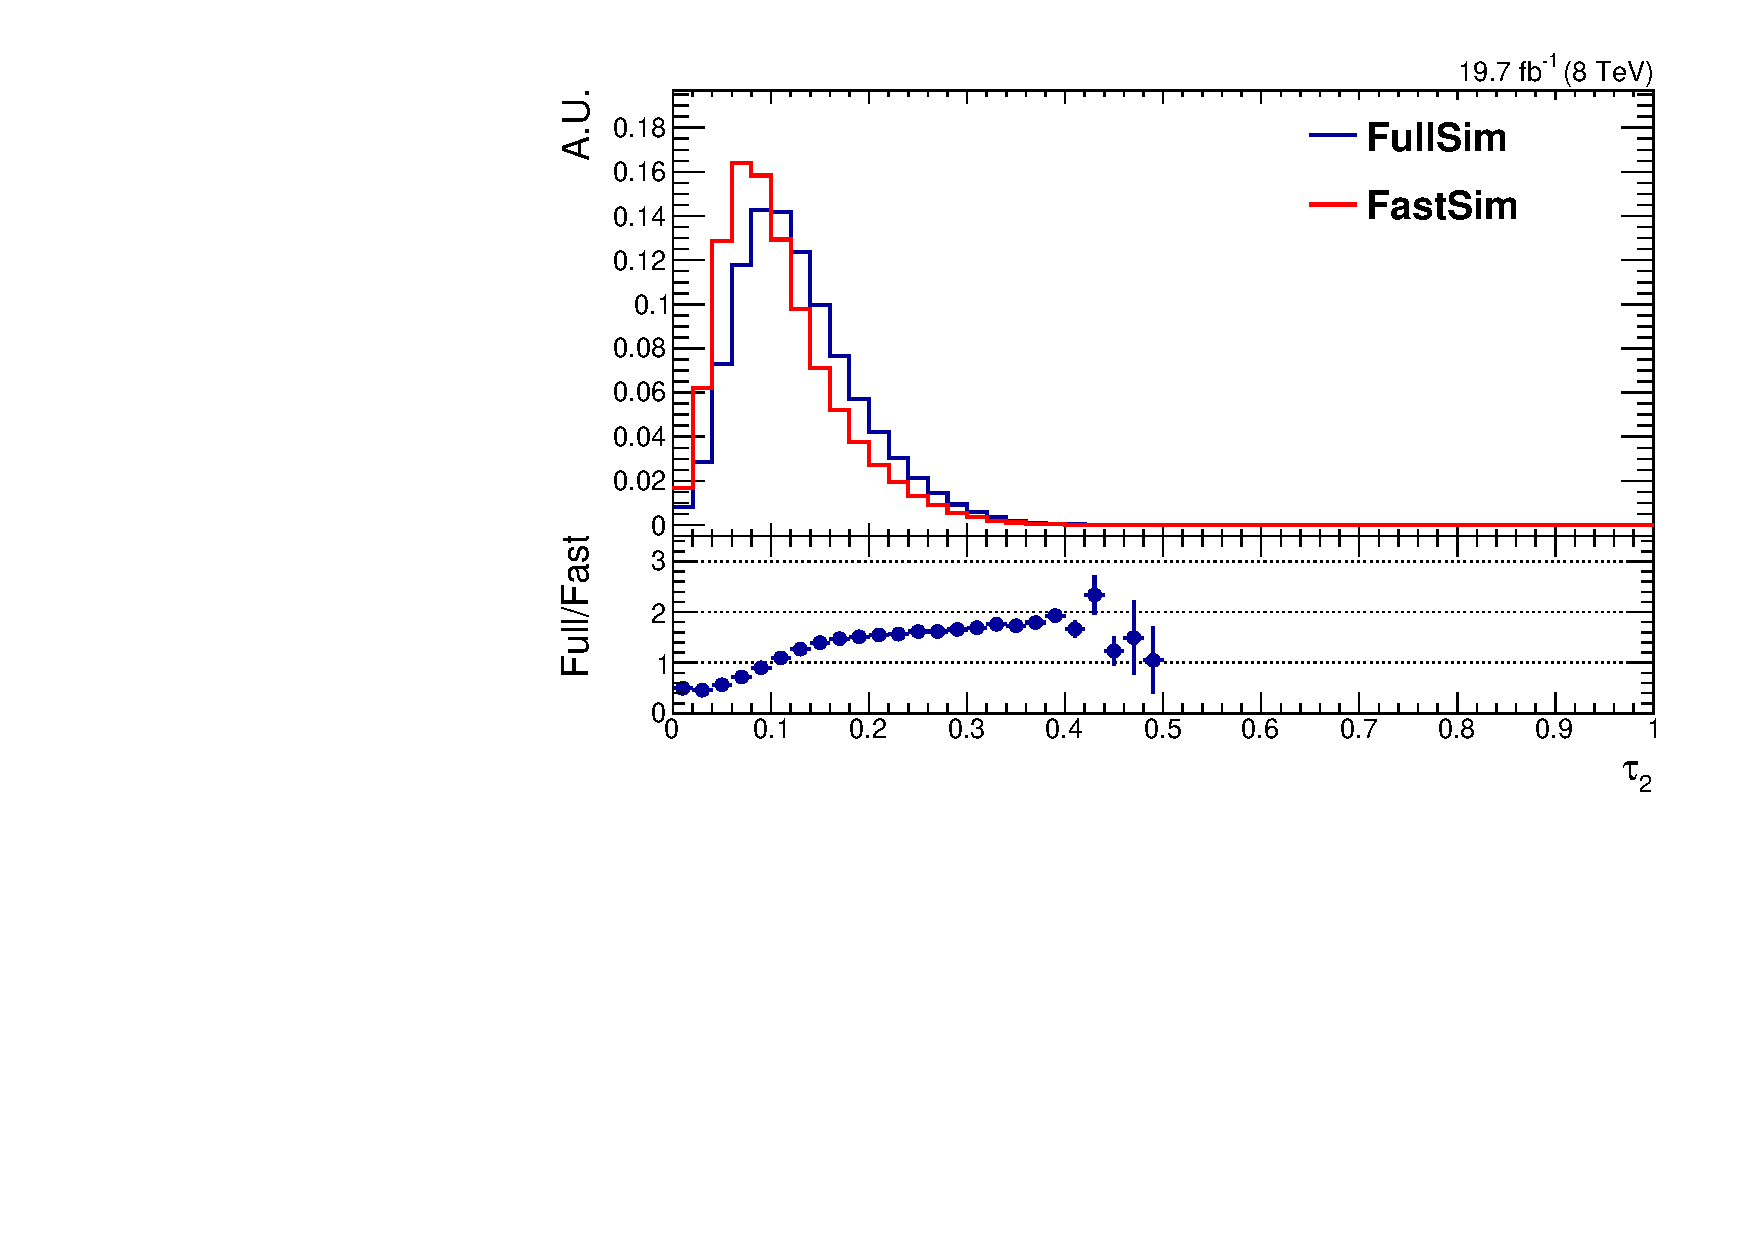
\includegraphics[width=0.49\textwidth]{figures/razor_wtag/FastFull_comparison_TTJets_tau2}
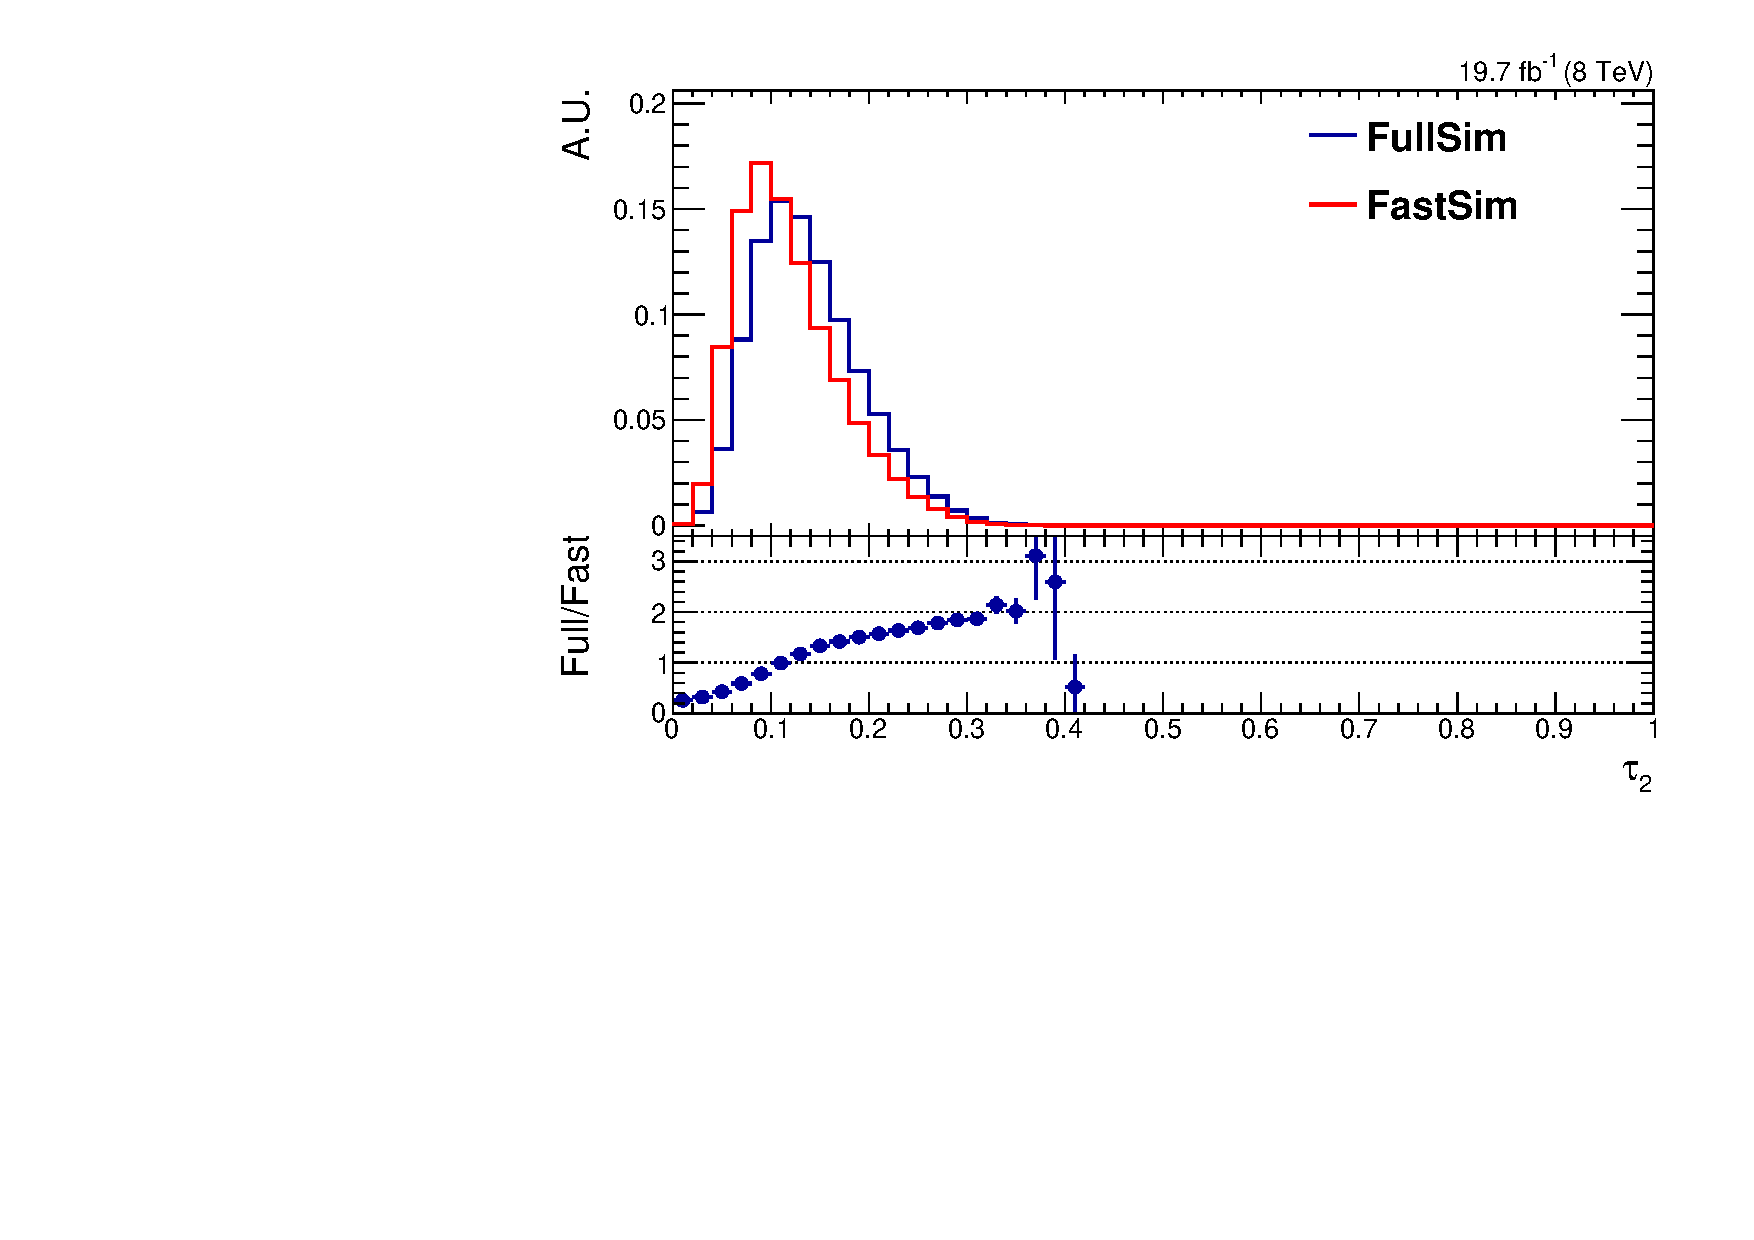
\includegraphics[width=0.49\textwidth]{figures/razor_wtag/FastFull_comparison_TTJets_tau2_masscut}
\caption{Distribution of $\tau_2$ before (left) and after (right) requiring the pruned CA8 jet to
lie within the $\W$ mass window, $70 < m_{\textrm{jet}} < 100$\GeV, for FastSim and FullSim
$t\bar{t}$.
\label{fig:FastFull_tau2}}
\end{figure}

\begin{figure}[p]
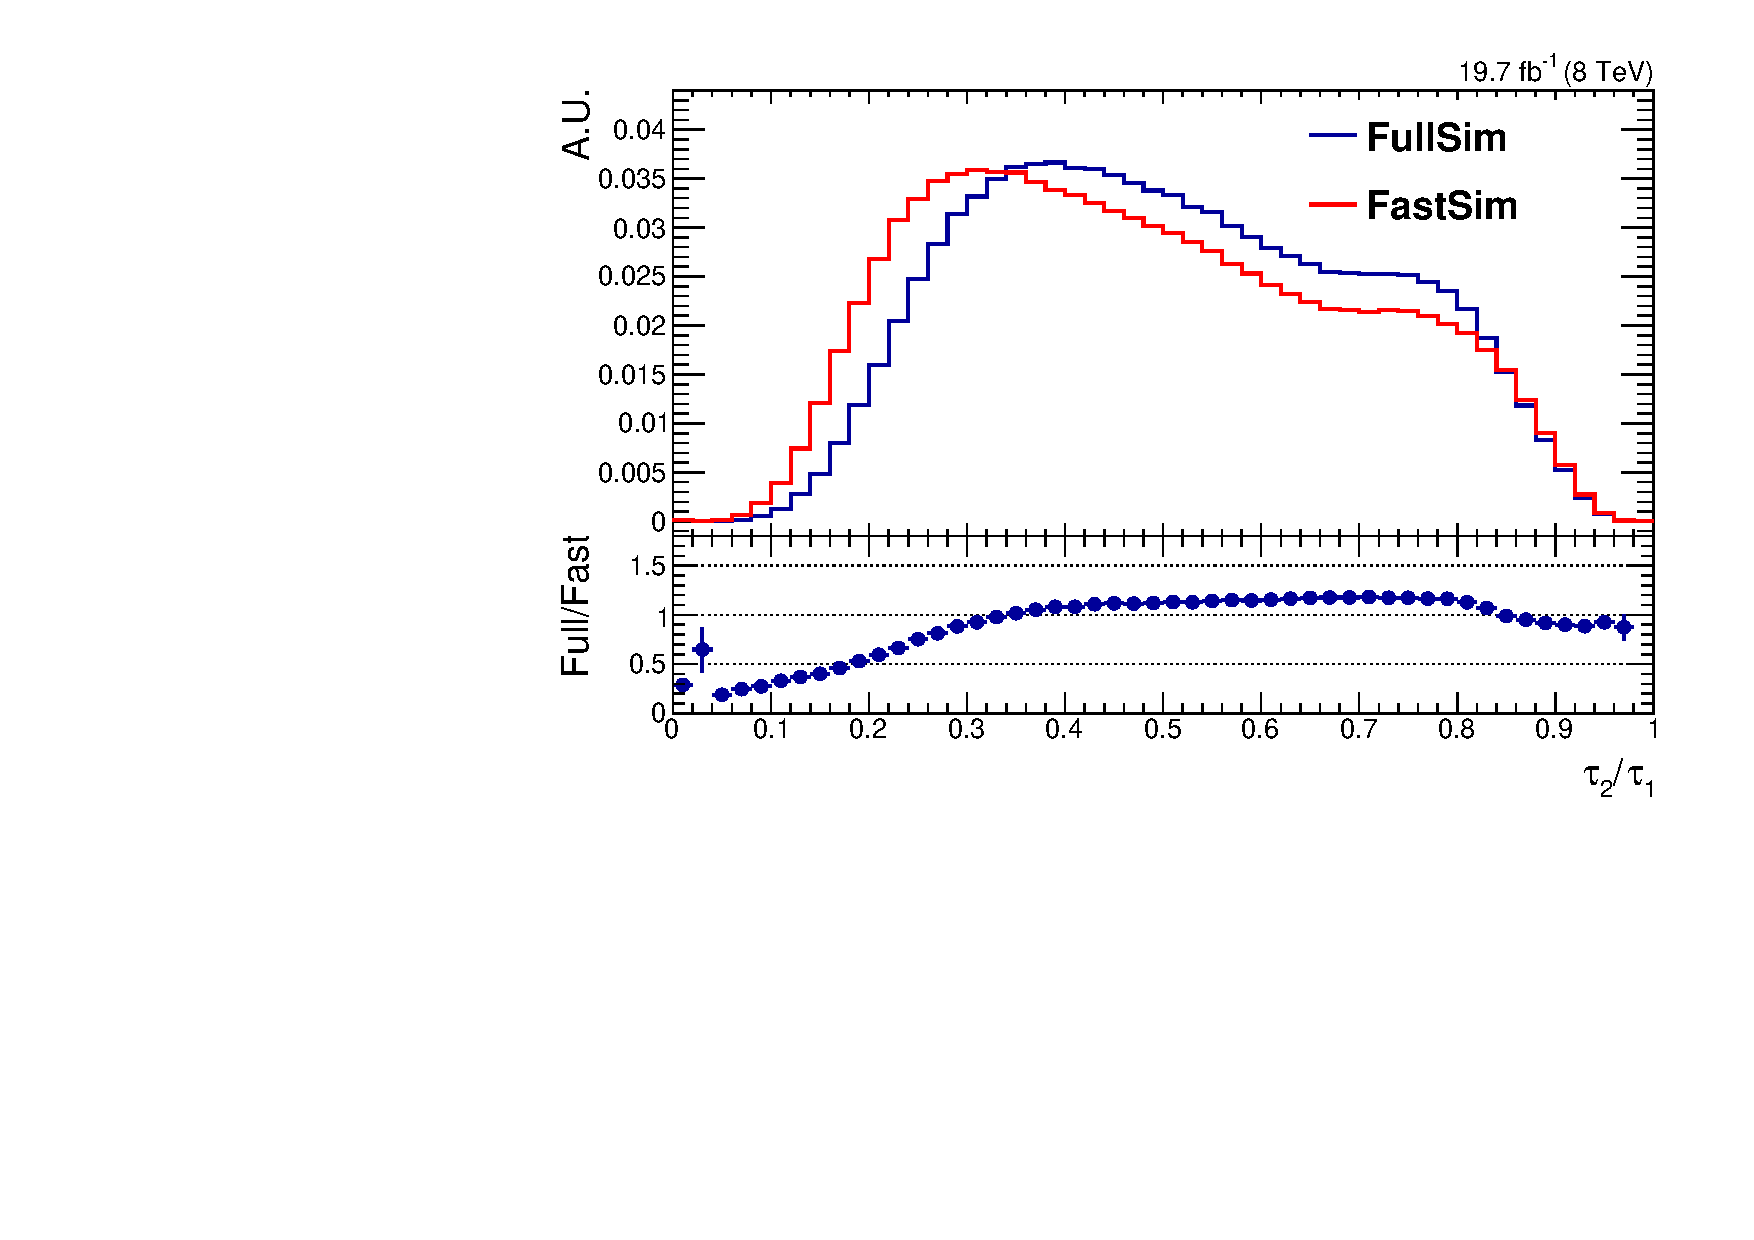
\includegraphics[width=0.49\textwidth]{figures/razor_wtag/FastFull_comparison_TTJets_tau21}
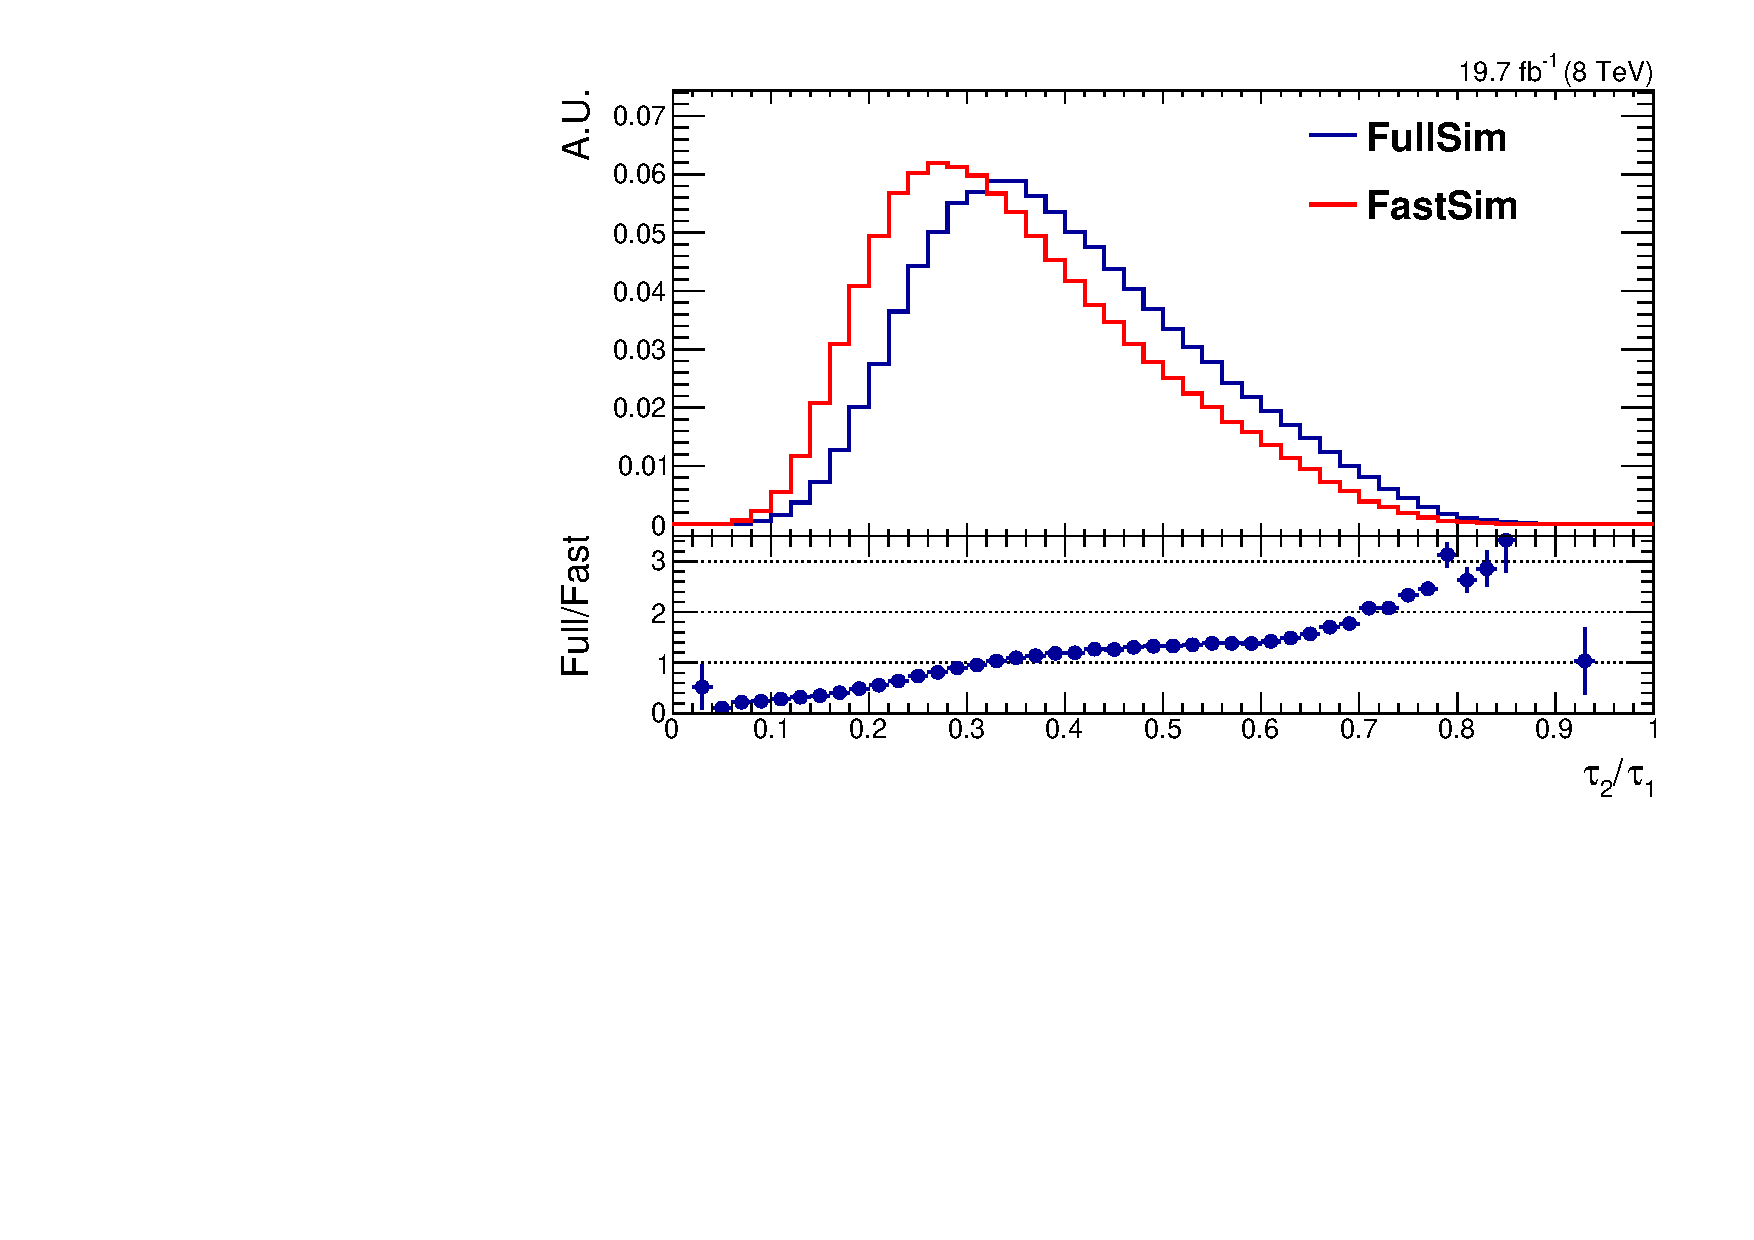
\includegraphics[width=0.49\textwidth]{figures/razor_wtag/FastFull_comparison_TTJets_tau21_masscut}
\caption{Distribution of $\tau_2/\tau_1$ before (left) and after (right) requiring the pruned CA8
jet to lie within the $\W$ mass window, $70 < m_{\textrm{jet}} < 100$\GeV, for FastSim and FullSim
$t\bar{t}$.
\label{fig:FastFull_tau21}}
\end{figure}

These figures also illustrate some of the features of the N-subjettiness variables.
Consider first the $\tau_1$ distribution in Fig.~\ref{fig:FastFull_tau1}. Without a jet mass
requirement, the distribution is quite broad and bimodal. Once the jet mass is required to
be consistent with the $\W$ boson mass, the lower part of the distribution disappears. This
illustrates that quark/gluon jets are expected to have only a single subjet, resulting in a small
$\tau_1$ value. For jets that result from the decay of a $\W$ boson, $\tau_1$ takes on a larger
value. 
This effect is not seen for the $\tau_2$ distributions (Fig.~\ref{fig:FastFull_tau2}), which is
expected because $\tau_2$ quantifies the compatibility with having two or fewer subjets. 
The ratio $\tau_2/\tau_1$, shown on Fig.~\ref{fig:FastFull_tau21}, also displays the
expected behaviour: the part of the distribution at high values is removed when requiring the jet
mass to be within the $\W$ mass window, and thus when selecting more jets with two-prong decays. 

The procedure to determine the $\W$ boson tagging efficiency for both FastSim and FullSim is the
following:
\begin{enumerate}
\item Filter the events at the generator level, requiring the presence of exactly one hadronically
decaying $\W$ boson. 
\item For the generated $\W$ boson, find the closest reconstructed CA8 jet, and require that it be
within $\Delta R = 0.8$ from the $\W$ boson. If no such jet exists, the event is discarded.  
\item Require that there be no (generator-level) $\cPqb$ quark from the top quark decay within the
cone of the selected CA8 jet. (We wish to select boosted $\W$ bosons only, not boosted top quarks.)
\item For the events that pass the above selection, consider the $\pt$ distribution of the CA8 jet
at two selection levels:
 \begin{itemize}
   \item no additional selection
   \item $70 < m_\textrm{jet} < 100$\GeV and $\tau_2/\tau_1 < 0.5$
 \end{itemize}
\item By dividing those \pt distributions we obtain the $\W$ boson tagging efficiency. 
\end{enumerate}
To derive the FullSim/FastSim scale factor for the $\W$ boson tagging efficiency, we divide the
efficiencies $\epsilon$ obtained in FullSim and FastSim:
\begin{equation}
SF_{\textrm{Full/Fast}}(\pt) =
\frac{\epsilon_{\textrm{FullSim}}(\pt)}{\epsilon_{\textrm{FastSim}}(\pt)}.
\end{equation}
A graphical representation of the $\W$ boson tag efficiency in FastSim and FullSim is shown on
Fig.~\ref{fig:boost_Wfullfast} for a fine and more coarse binning in CA8 jet \pt. The resulting
scale factor is shown for the final, coarse binning that will be used to rescale the signal
simulation. 
Table~\ref{tab:SF_FullFast} summarizes the $\W$ boson tag efficiency FullSim/FastSim scale factor
with its
statistical uncertainty.

\begin{figure}[htbp]
\centering
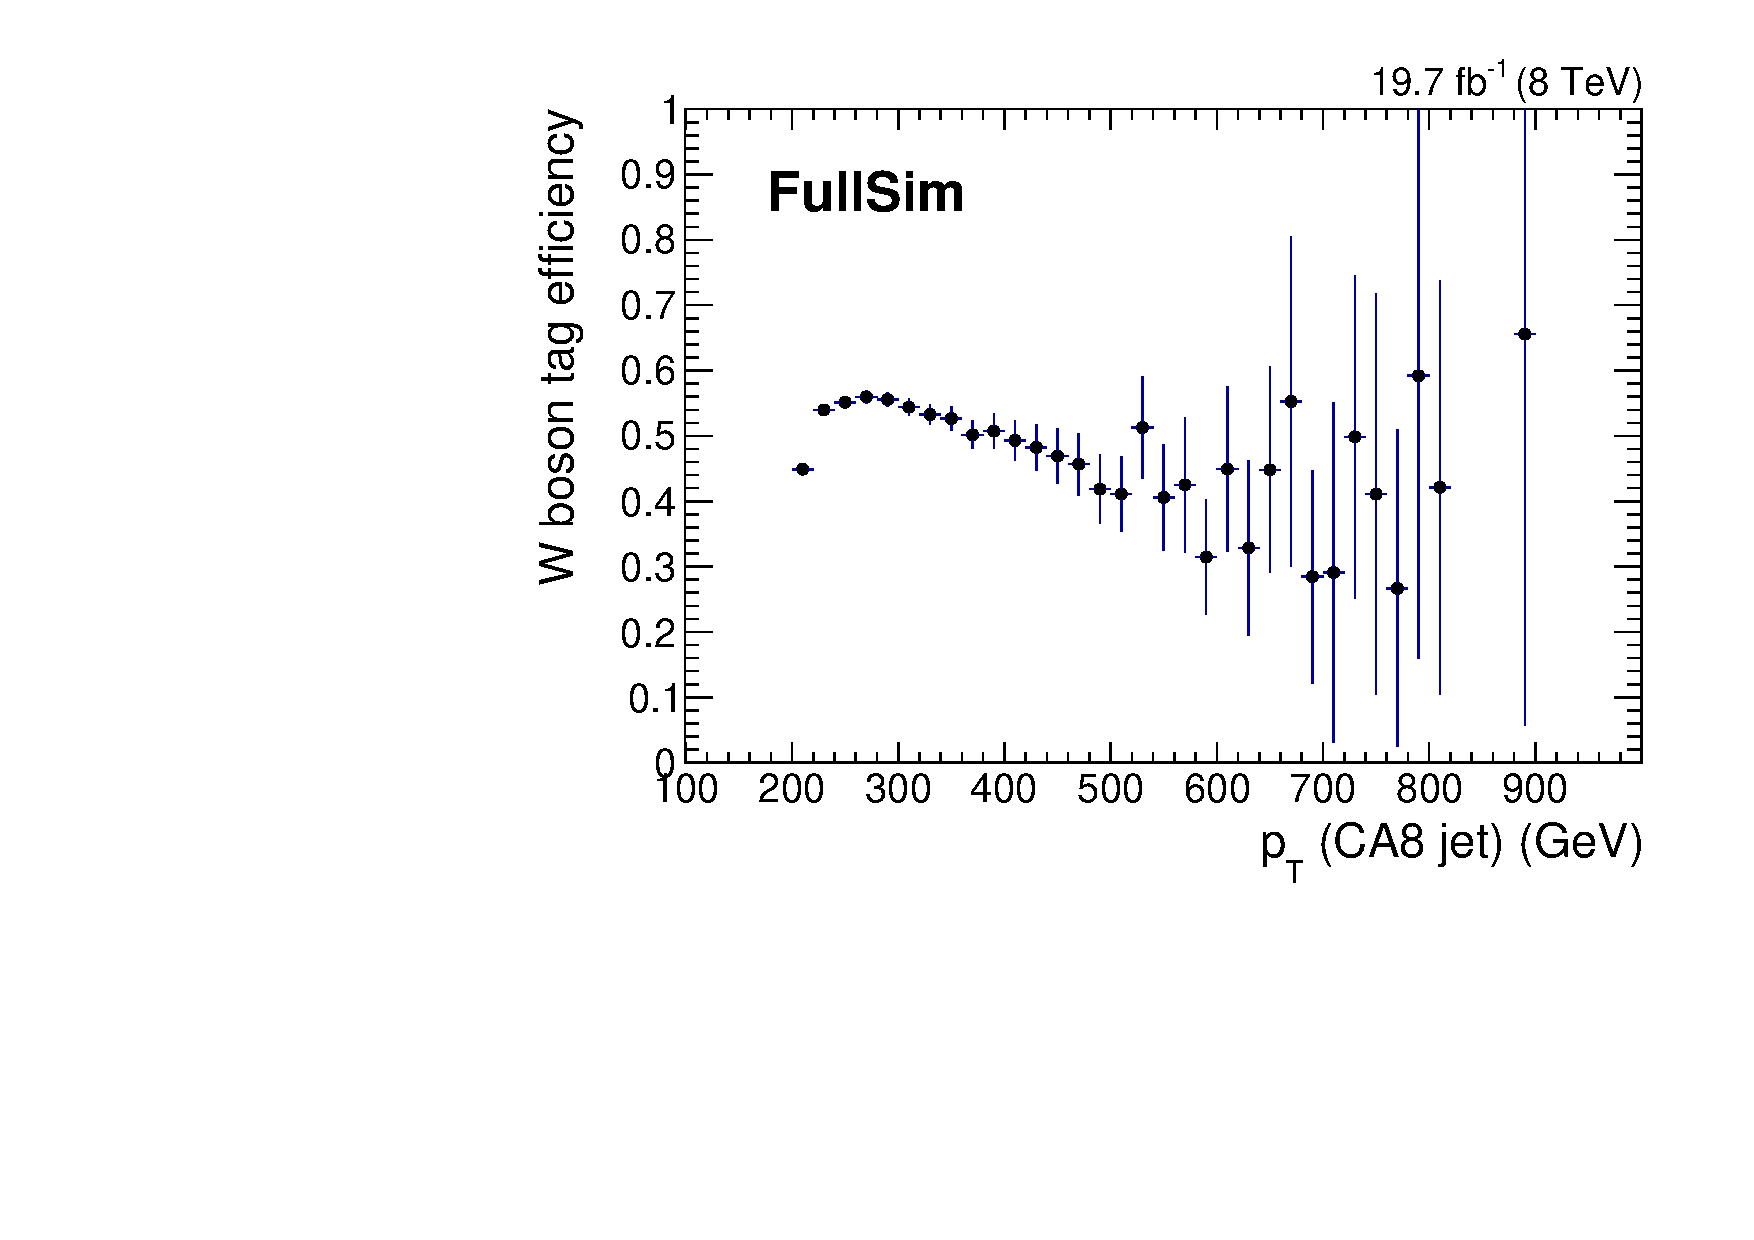
\includegraphics[width=0.48\textwidth]{figures/razor_wtag/Eff_ratio_tagged_all_FullSim_Thesis}
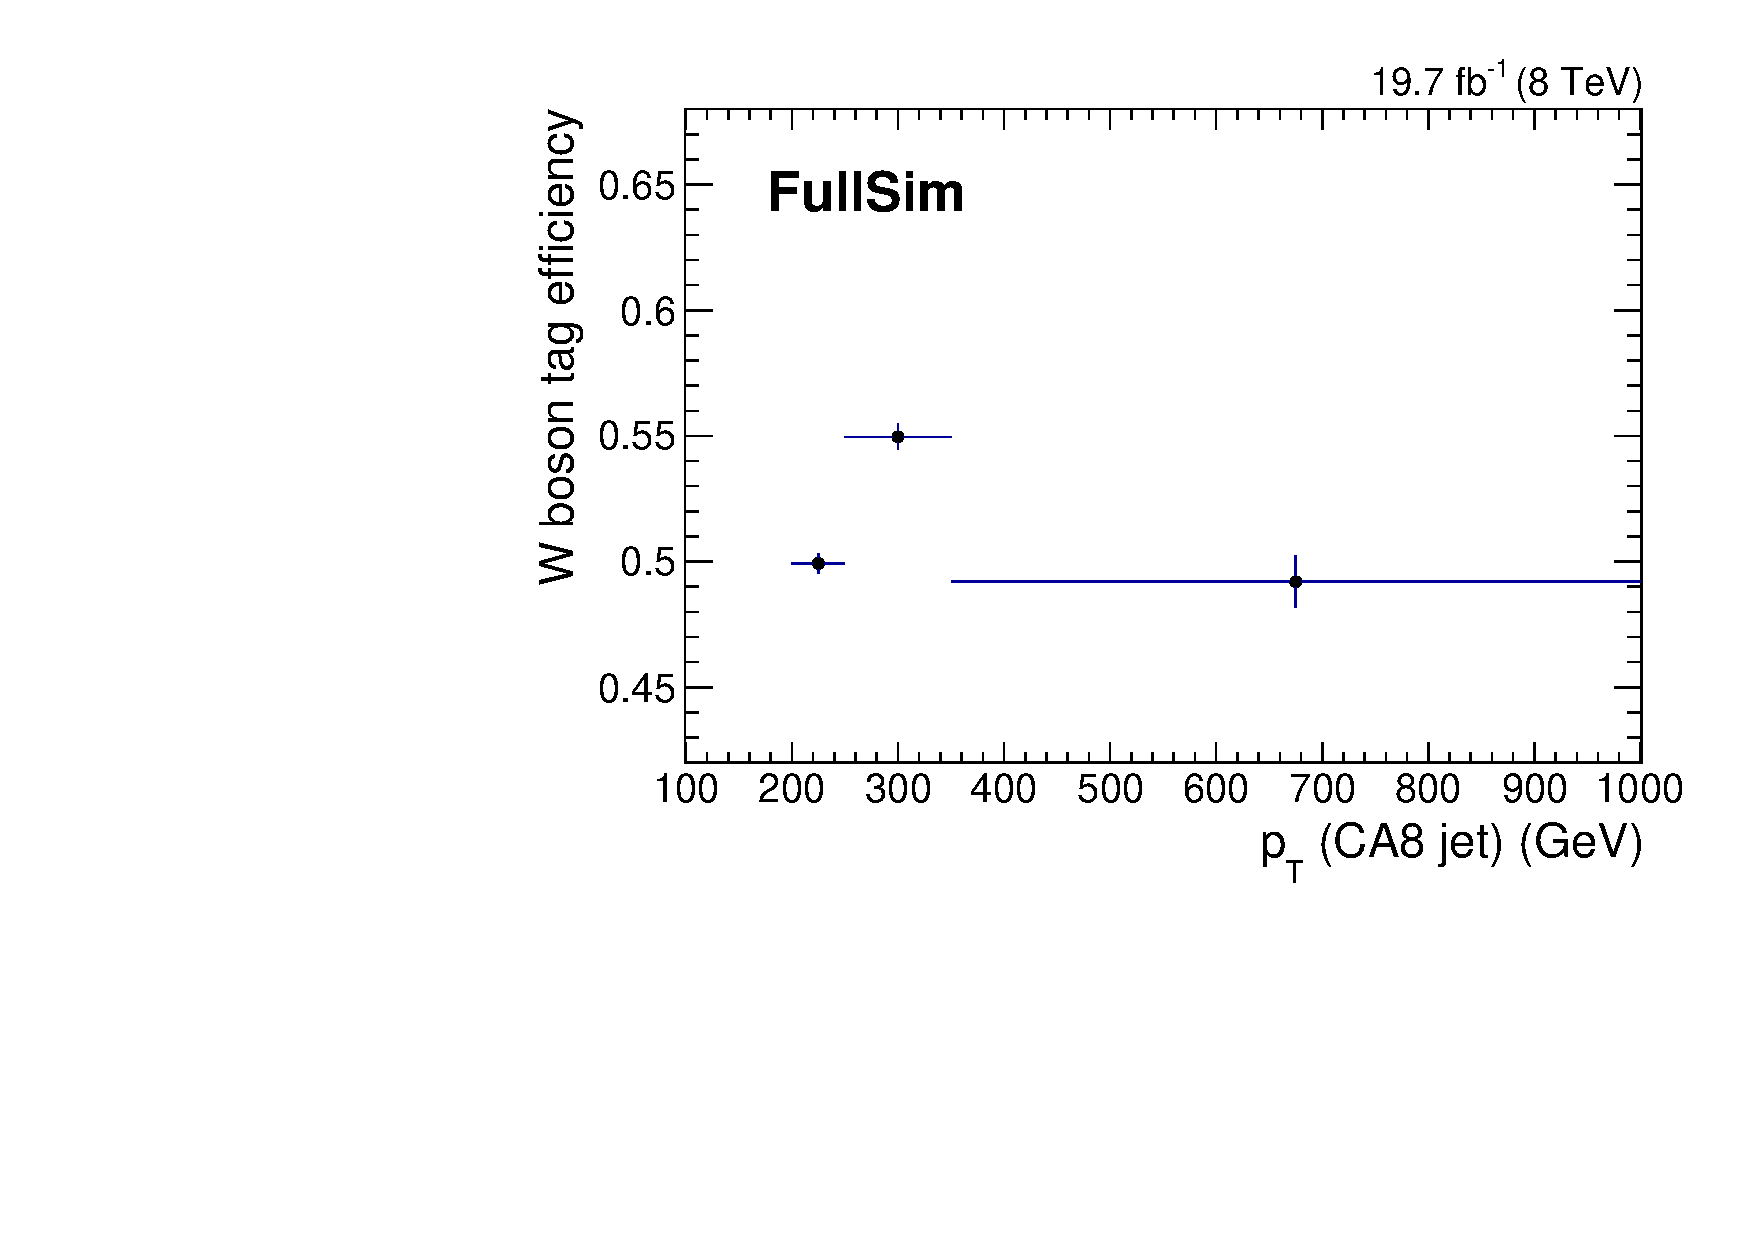
\includegraphics[width=0.48\textwidth]
{figures/razor_wtag/Eff_ratio_tagged_all_varbin_FullSim_Thesis}

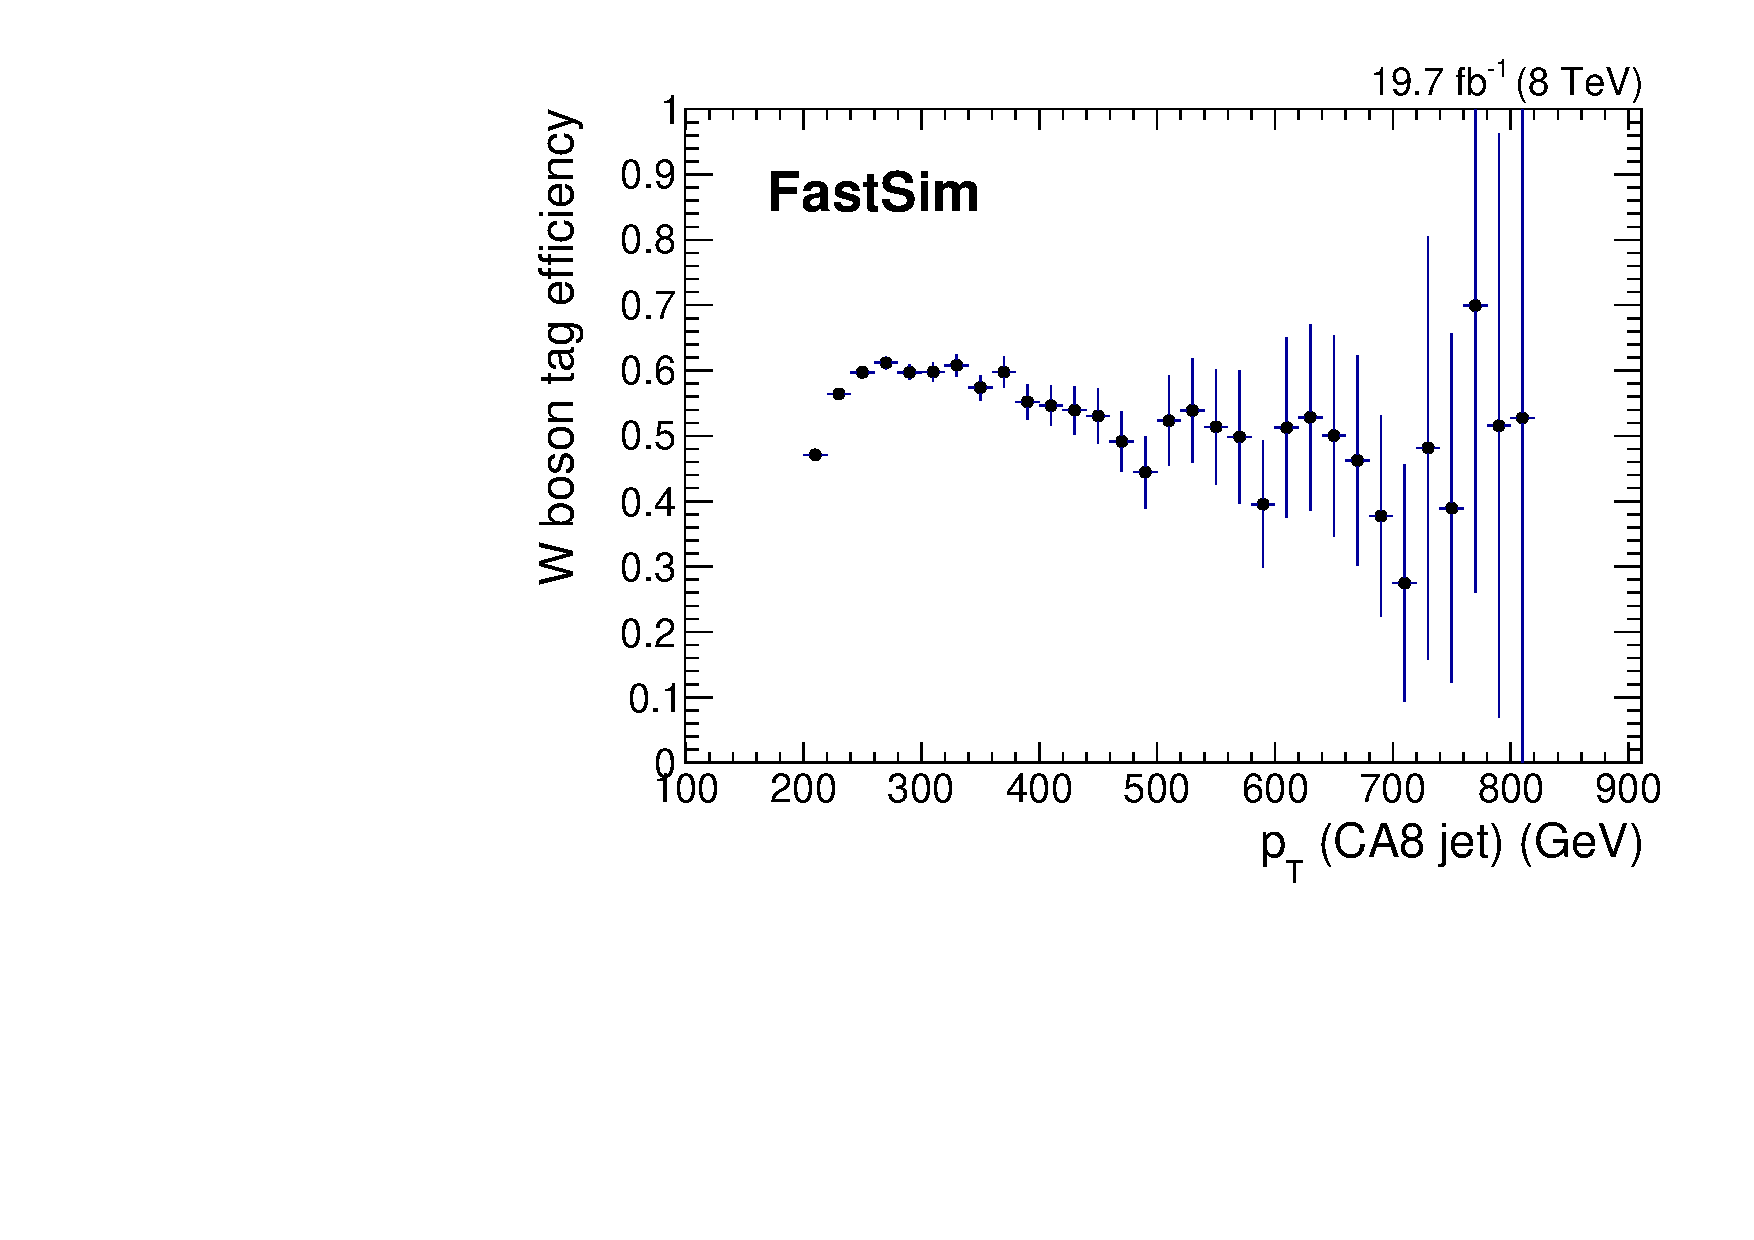
\includegraphics[width=0.48\textwidth]{figures/razor_wtag/Eff_ratio_tagged_all_FastSim_Thesis}
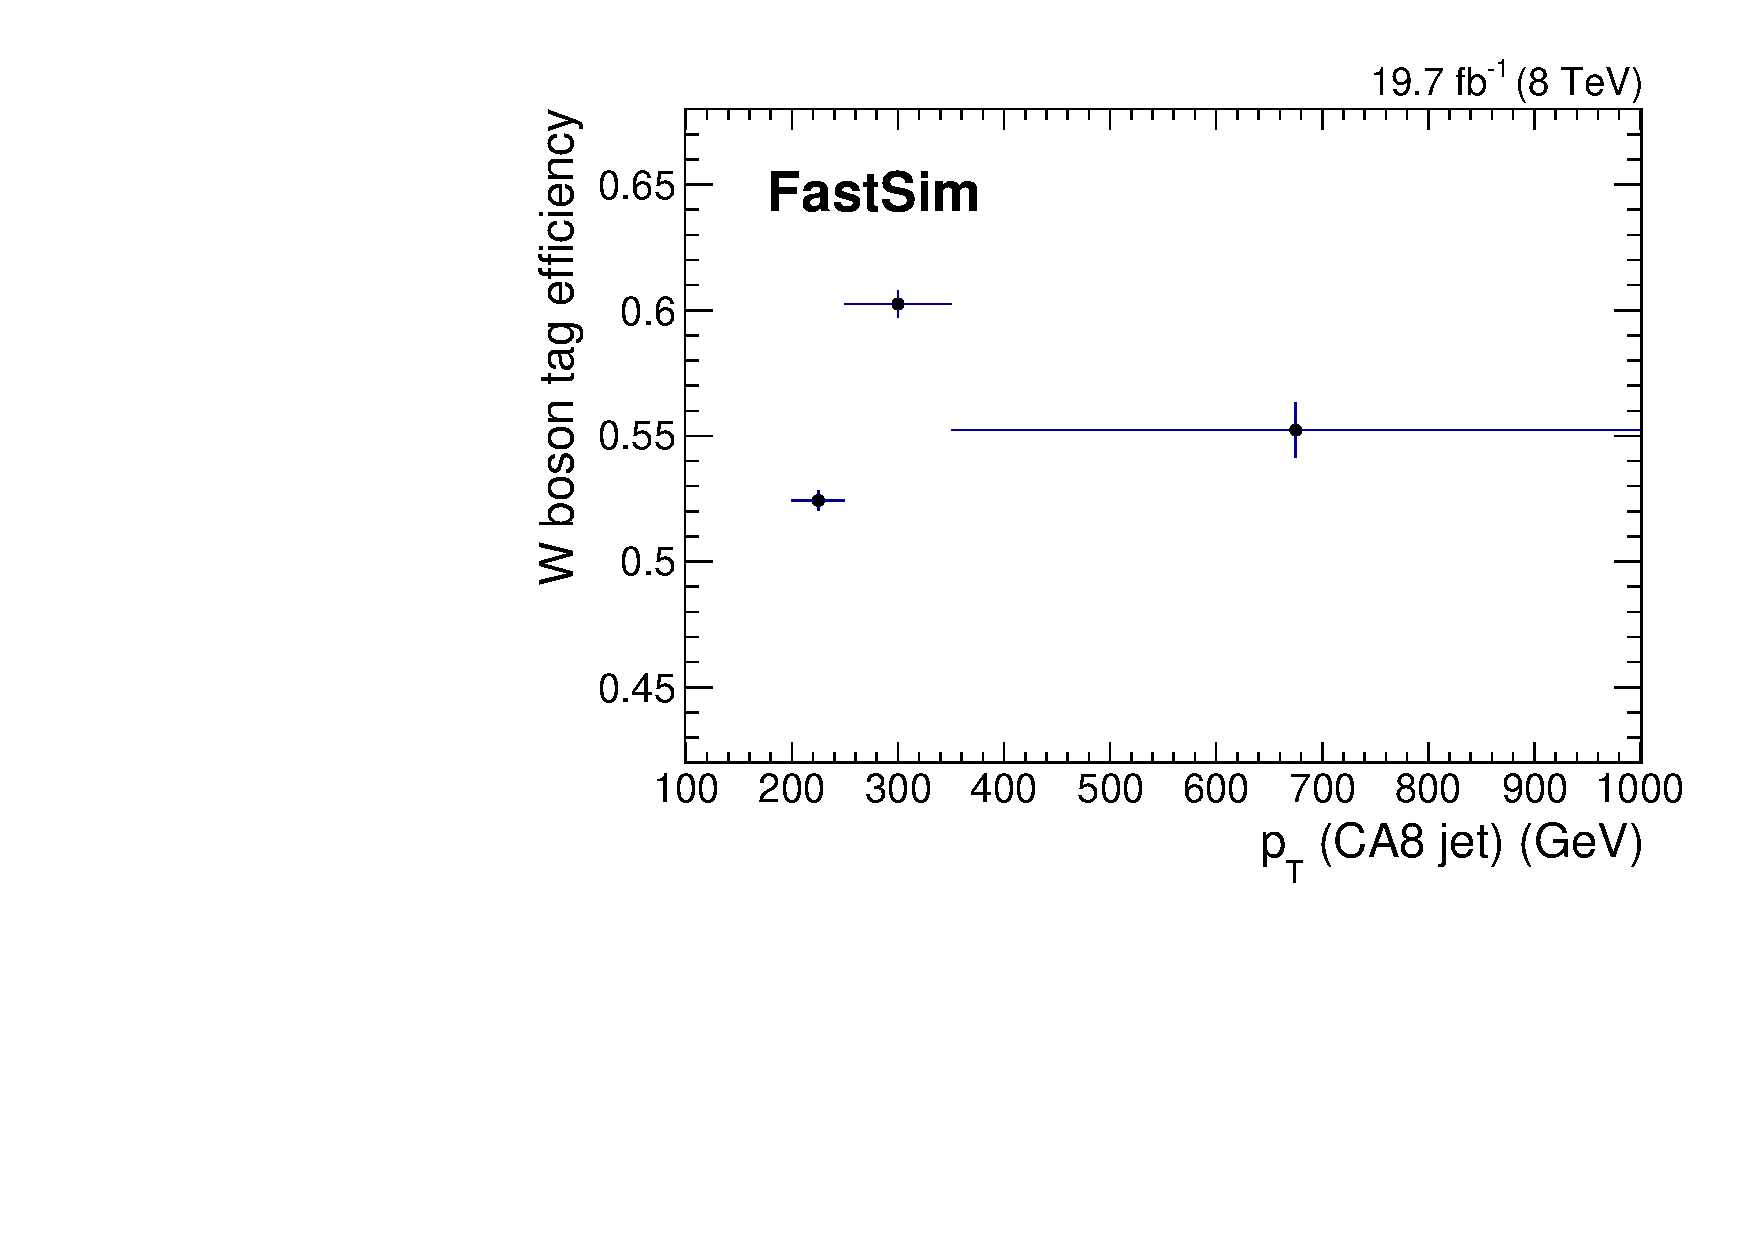
\includegraphics[width=0.48\textwidth]
{figures/razor_wtag/Eff_ratio_tagged_all_varbin_FastSim_Thesis}

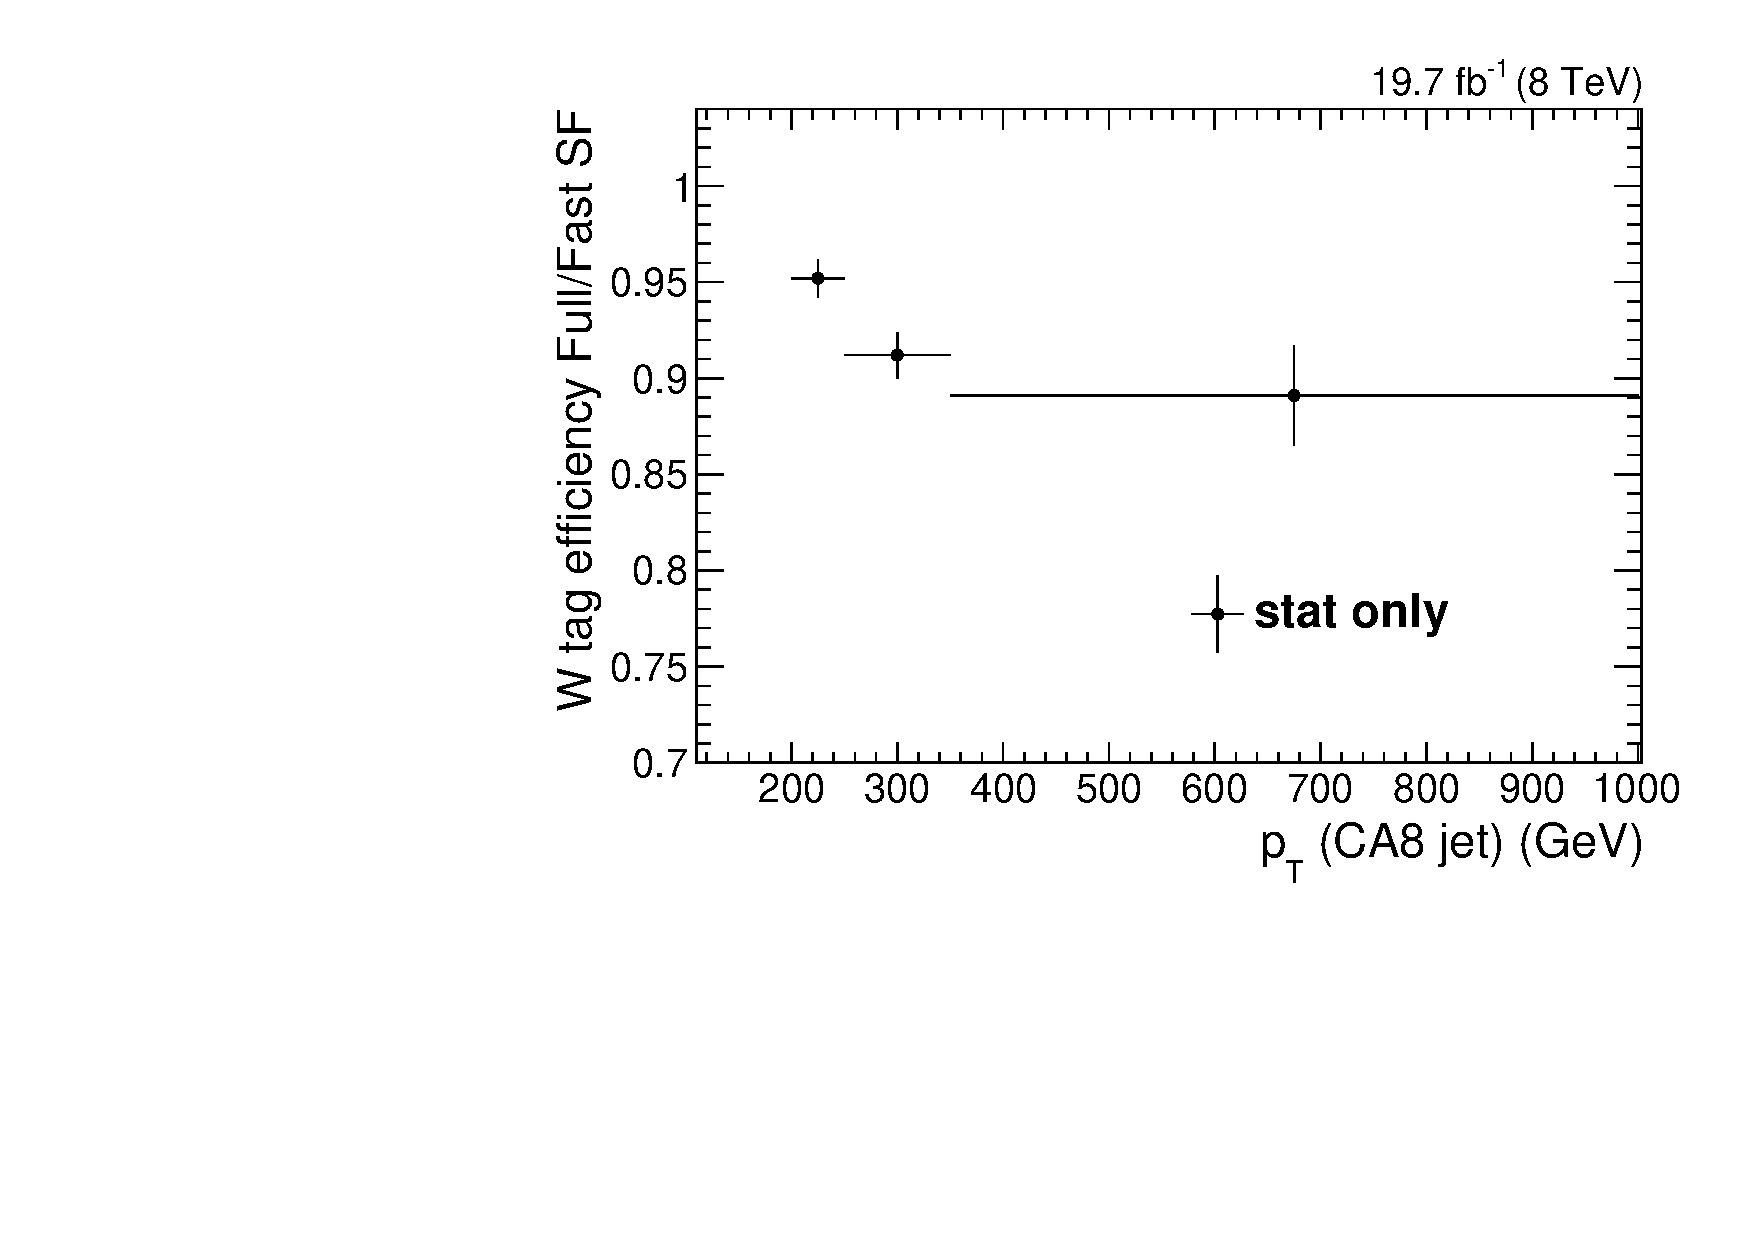
\includegraphics[width=0.6\textwidth]{figures/razor_wtag/SF_FullFast_Thesis}
\caption{[top] $\W$ boson tag efficiency versus CA8 jet \pt, with two different binnings, obtained
from FullSim $t\bar{t}$ events as described in the text. The shown uncertainties are statistical
only. 
[middle] $\W$ boson tag efficiency versus CA8 jet \pt, with two different binnings, obtained from
FastSim $t\bar{t}$ events as described in the text. The shown uncertainties are statistical only. 
[bottom] $\W$ boson tag FullSim/FastSim efficiency scale factor versus CA8 jet \pt. The shown
uncertainties are statistical only.
\label{fig:boost_Wfullfast}}
\end{figure}

\begin{table}[htpb]
\centering
\caption{Summary of FullSim/FastSim scale factor for the $\W$ tag efficiency.}
\vspace{1ex}
\begin{tabular}{c c}
\toprule
CA8 jet $\pt$ (\GeV) & $SF_{\textrm{Full/Fast}}$\\
\midrule
$[200 - 250[$ &  $0.952 \pm 0.010$ \\
$[250 - 350[$ &  $0.912 \pm 0.012$ \\
$[350 - ...]$ &  $0.891 \pm 0.026$ \\
\bottomrule
\end{tabular}
\label{tab:SF_FullFast}
\end{table}

%% ---------------------------------------------------------------------------------------------

\subsubsection{\texorpdfstring{$\W$}{W} boson tag fake rate scale factor \label{sec:wtag_fake_sf}}

The $\W$ boson tag fake rate scale factor is meant to correct processes that do not have
hadronically decaying $\W$ bosons in their final state. As the fake rate depends on the composition
of the sample, this scale factor has to be derived for each analysis separately. 
We will thus need to obtain a sample of events containing misidentified $\W$ boson jets to derive a
dedicated scale factor for the razor boost analysis. A multijet-enriched control region is defined,
using the following selection:
\begin{itemize}
\item no loose leptons, 
\item no $\cPqb$ tagged (CSVL) jets,
\item at least 3 AK5 jets,
\item at least one AK5 jet with $\pt>200$\GeV,
\item small minimum azimuthal angle between the \VEtmiss and the leading three jets, \\
$\Delta\phi_{min} < 0.3$.
\end{itemize}
This selection is similar to the baseline selection employed in the rest of the analysis. The
kinematic regime, and the composition of the sample will thus also be similar. The main difference
is that we have not applied any selection on the razor variables \mr or \rsq, in order to retain a
higher statistical power. 

To obtain the fake rates $\epsilon$ for $\W$ boson tagging we use the leading CA8 jet in each
event, and check whether it is tagged by the $\W$ boson tagger. After obtaining the
fake rates in both data and simulation, we compute the scale factor as their ratio,
\begin{equation}
SF_\textrm{Wtag}^\textrm{fake}(\pt) =
\frac{\epsilon^{\textrm{data}}(\pt)}{\epsilon^{\textrm{simulation}}(\pt)}.
\end{equation} 
In the calculation of the uncertainties on this scale factor we include the statistical uncertainty,
as well as the trigger efficiency and jet energy scale uncertainties for both AK5 and CA8 jets. 
All three uncertainties are varied up (down) at the same time to get the overall up (down)
systematic  uncertainty.
The fake rate in data and simulation, as well as the resulting $\W$ boson tag fake rate scale factor
are shown in Fig.~\ref{fig:boost_wfake}. As we can see from the figure, there is a drop in the scale
factor just above a \pt of 300\GeV. This is a result of a residual mismodelling of the trigger
efficiency. 

%\textcolor{red}{TODO: add more information on this "wiggle", perhaps in an appendix.}

\begin{figure}[htbp]
\centering
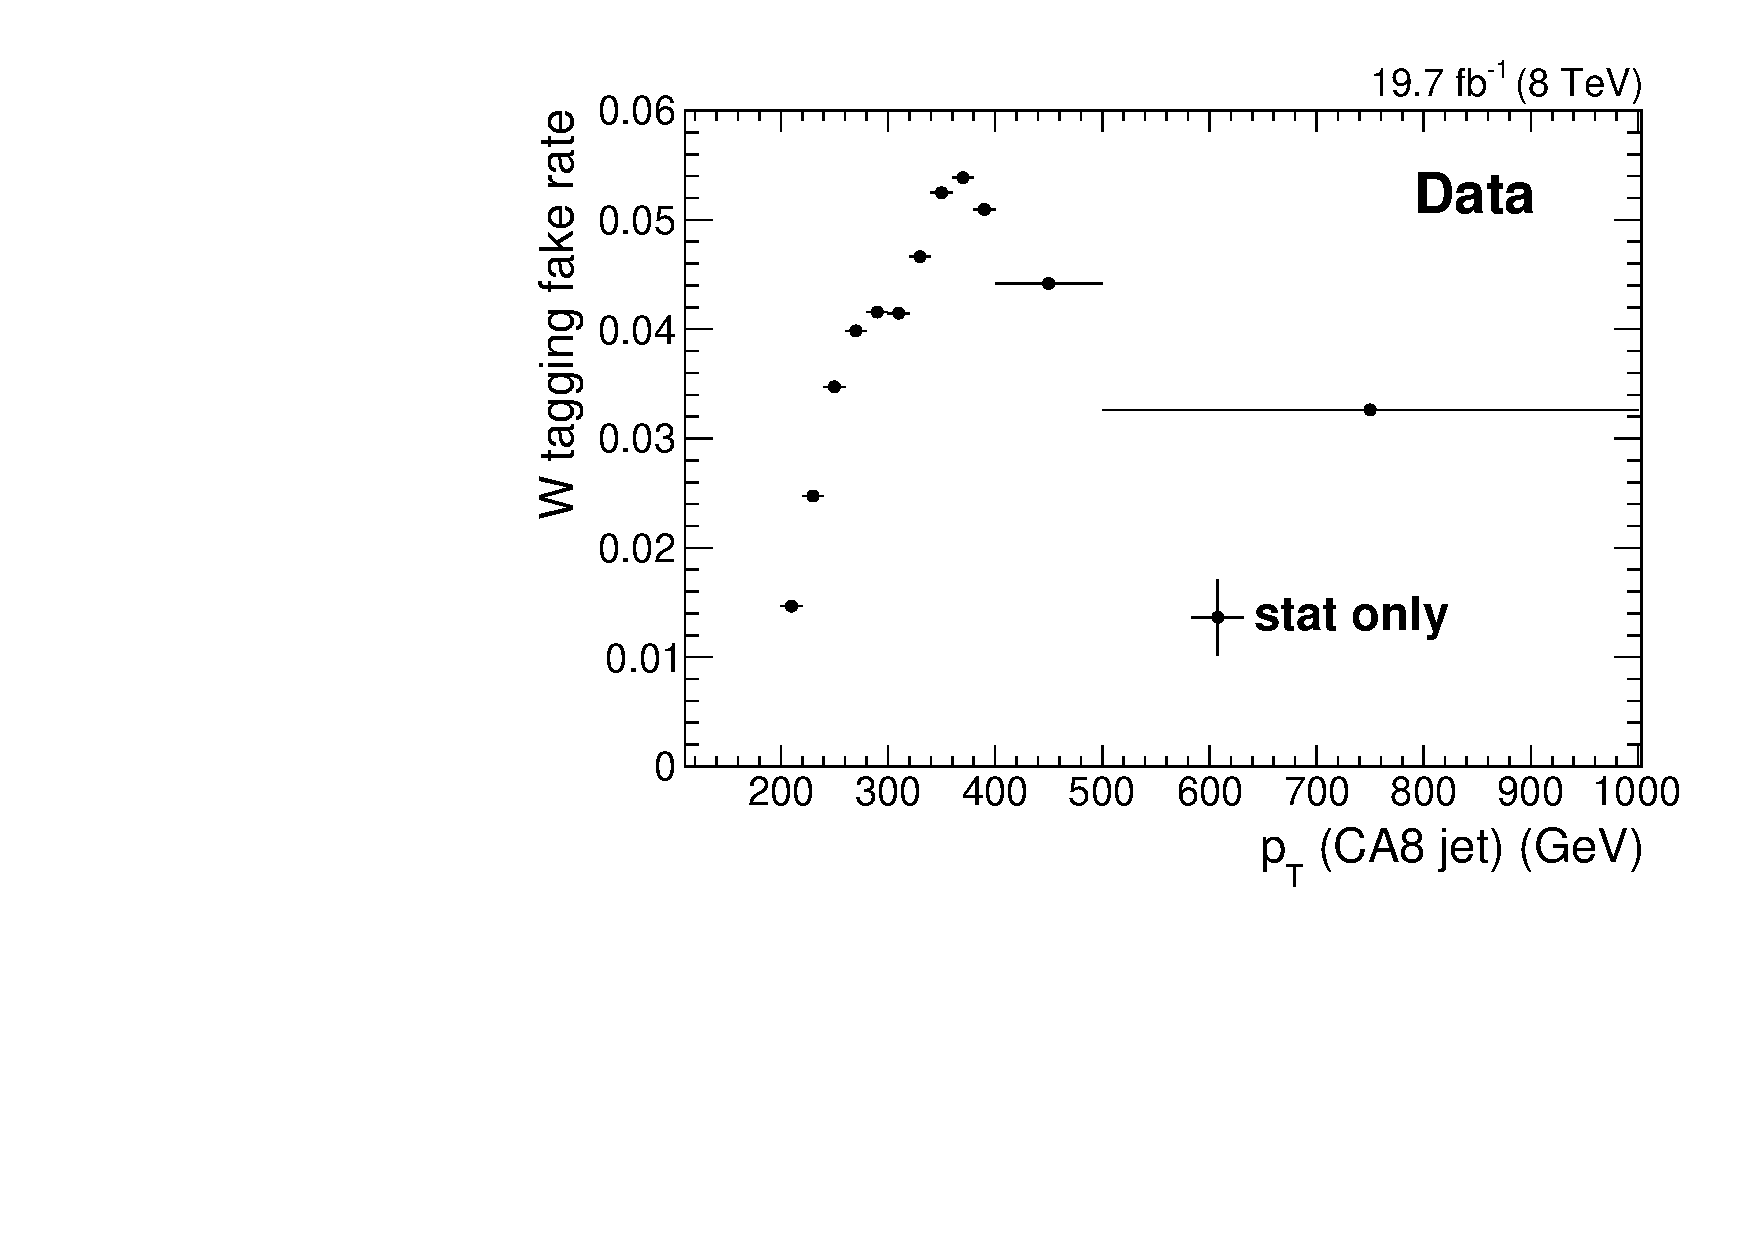
\includegraphics[width=0.6\textwidth]{figures/razor_wtag/Eff_Data_ratio_pt_tagged_all_Data_Thesis}

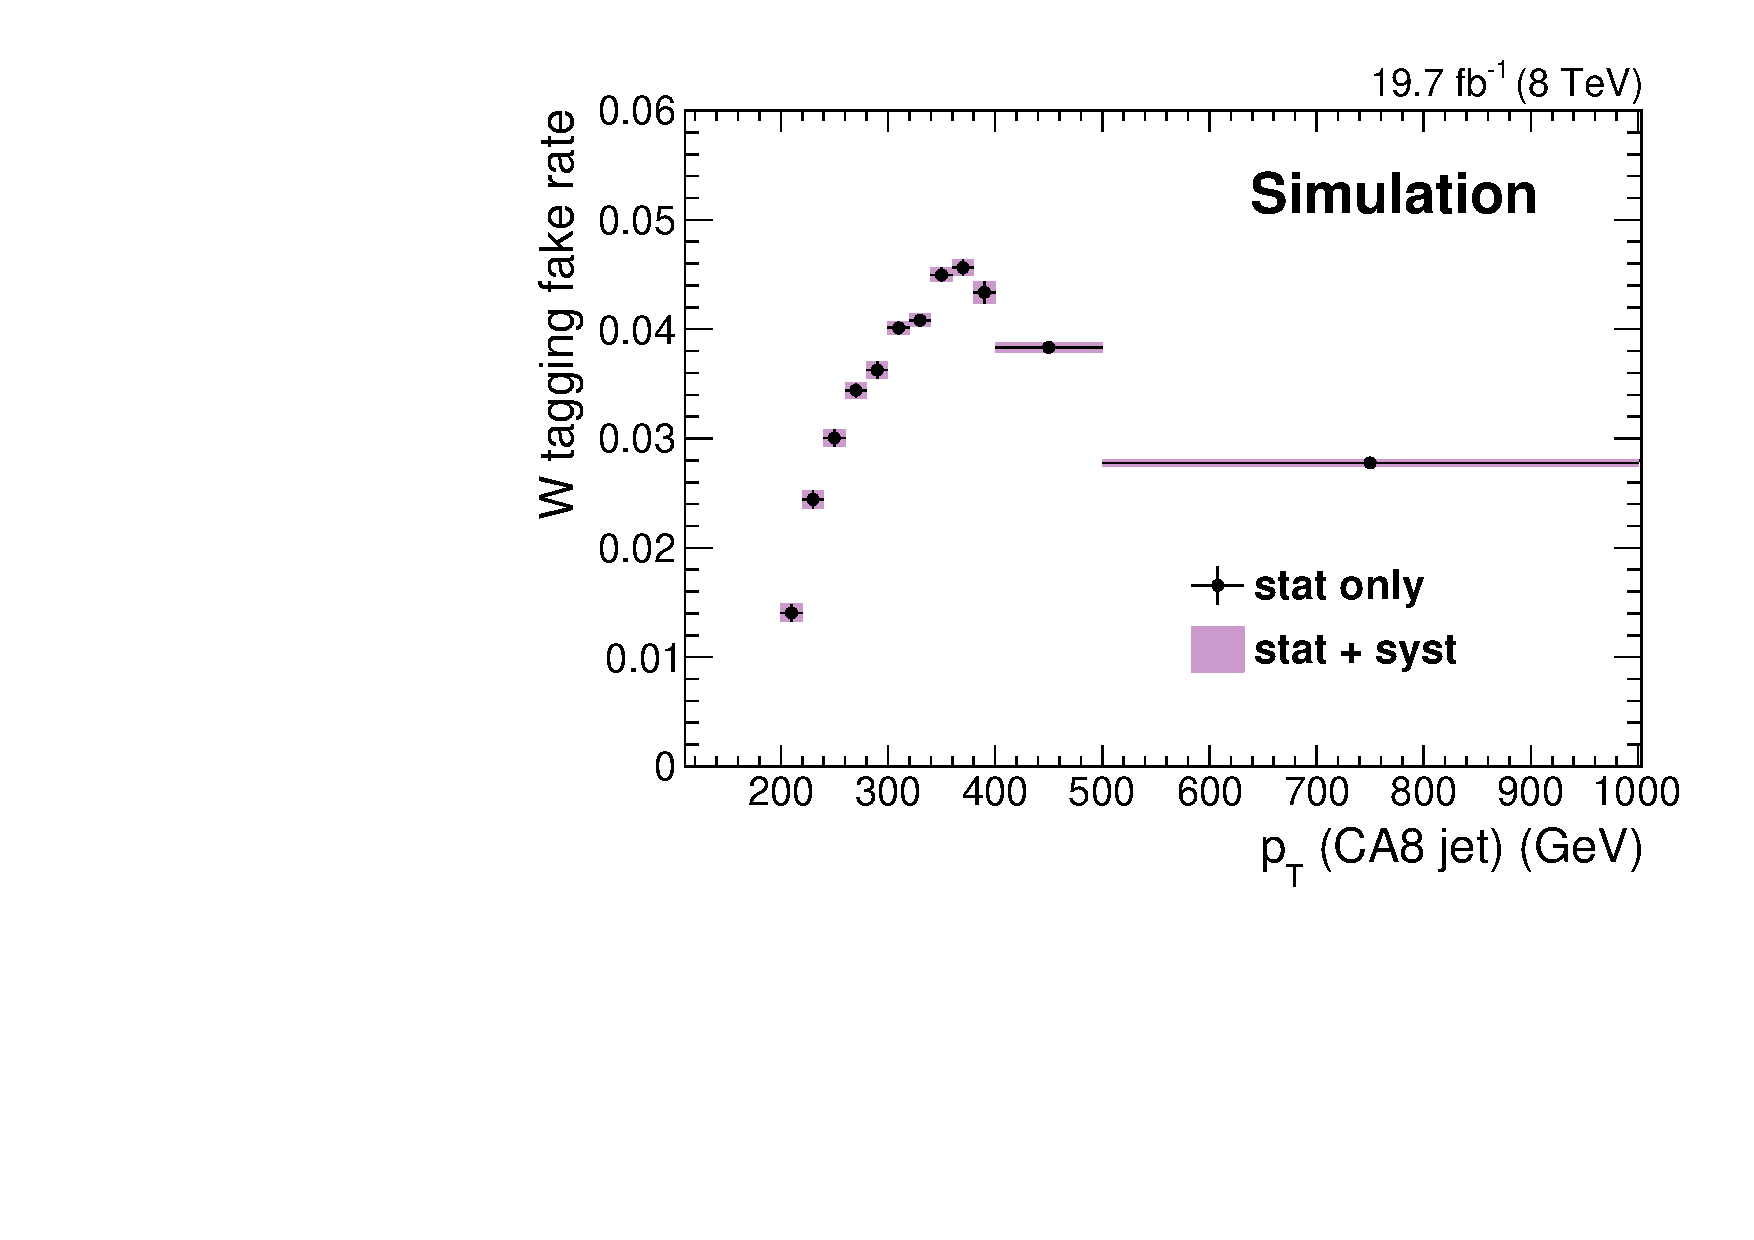
\includegraphics[width=0.6\textwidth]{figures/razor_wtag/Eff_MC_ratio_pt_tagged_all_MC_Thesis}

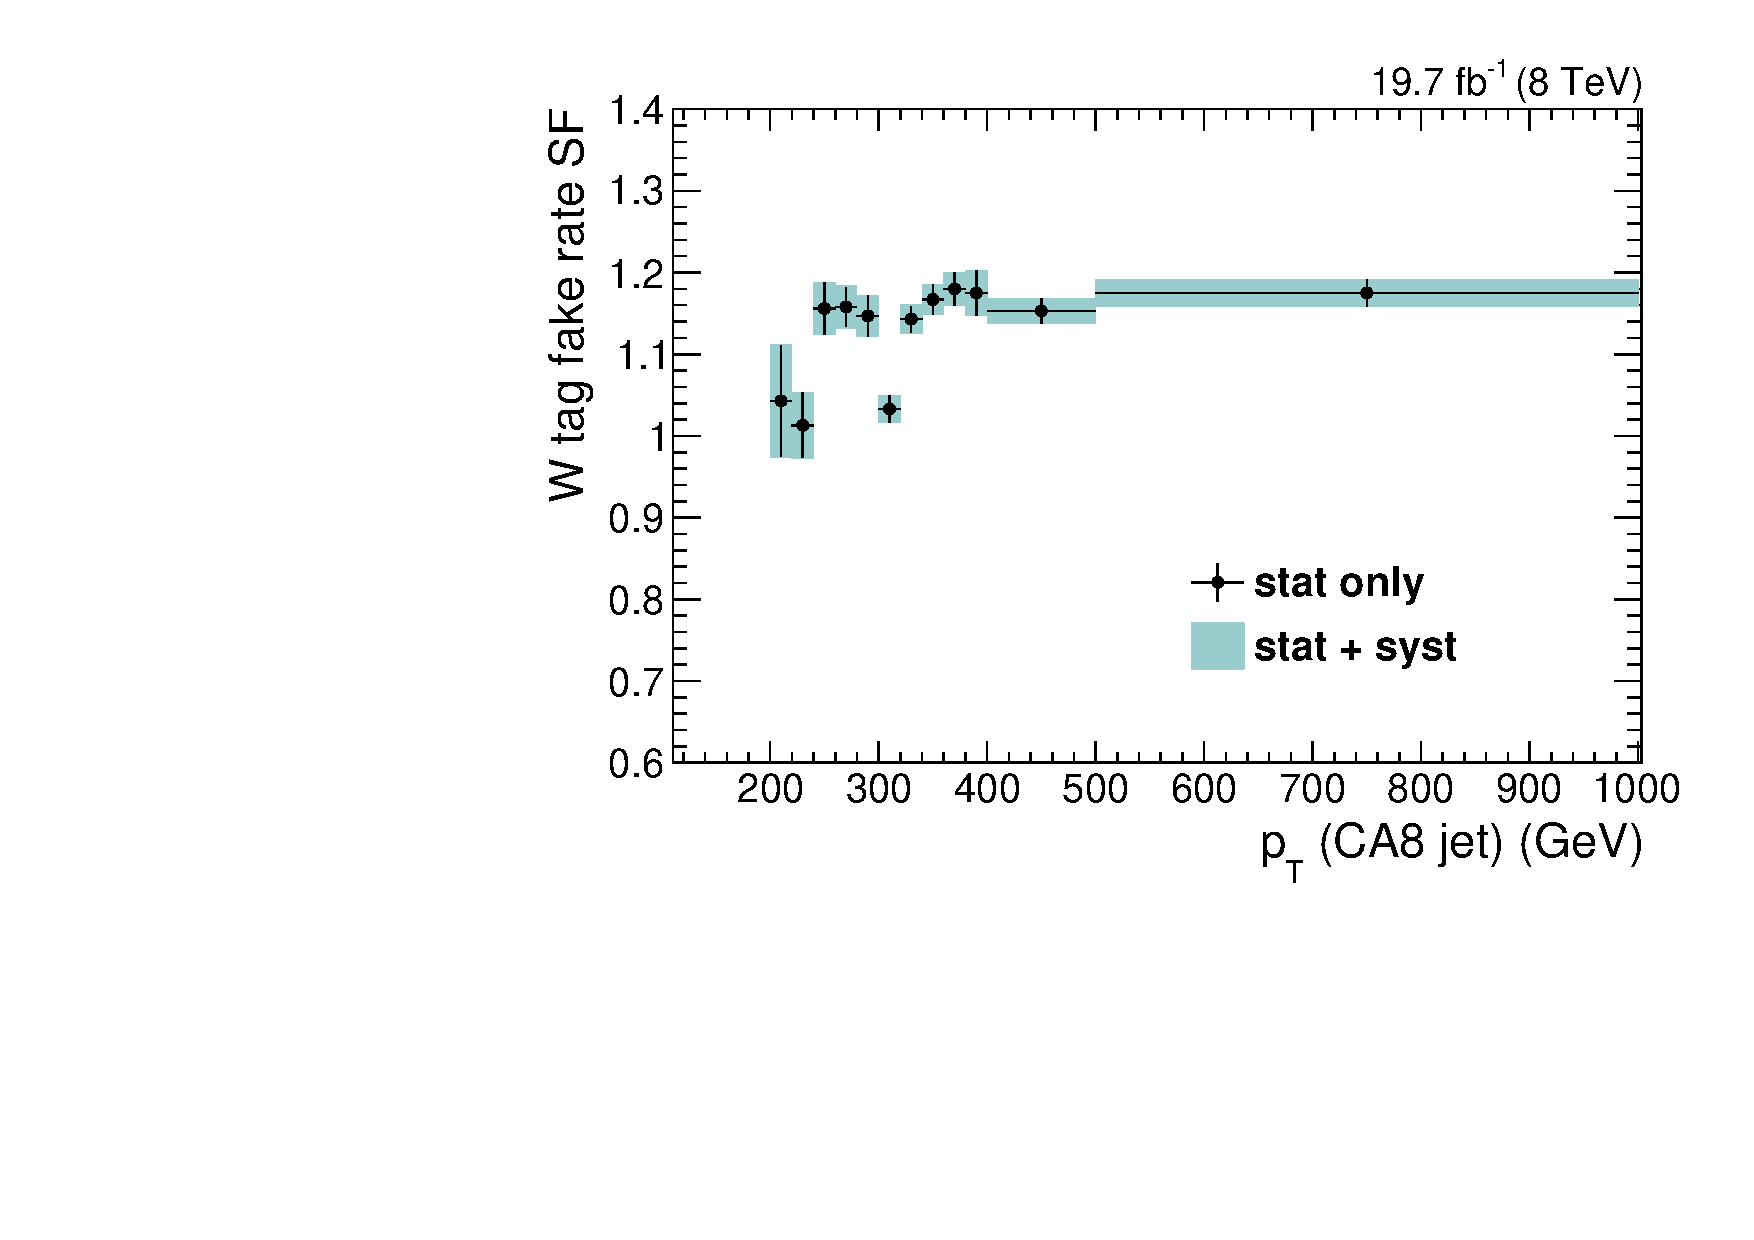
\includegraphics[width=0.6\textwidth]{figures/razor_wtag/SF_Wfake_Thesis}
\caption{[top] Misidentification probability according to $\W$ tagging for a CA8 jet versus
jet \pt obtained from a multijet-enriched control region in data as described in the text. The shown
uncertainties are statistical only. 
[middle] $\W$ boson tag fake rate obtained from simulation. The uncertainty band includes
statistical and systematic uncertainties.
[bottom] Scale factor for $\W$ tag fake rate versus CA8 jet \pt obtained from a
multijet-enriched control region as described in the text. The uncertainty band includes
statistical and systematic uncertainties.
\label{fig:boost_wfake}}
\end{figure}

The $\W$ boson tag fake rate scale factor is applied in the $S$ and $T$ region, as is the case for
the $\W$ boson tag efficiency scale factor. It is applied to all simulated samples without real
hadronically decaying $\W$ bosons, such as multijet production, $W(\rightarrow\ell\nu)$+jets,
$\cPZ/\gamma^*(\rightarrow\ell\ell)$+jets, etcetera. 

%% ---------------------------------------------------------------------------------------------

\subsubsection{\texorpdfstring{$\W$}{W} boson mass-tag fake rate scale factor
\label{sec:wmasstag_fake_sf}}

This scale factor corresponds to the $\W$ boson mass-tagging definition, which will be used in the
$W$ control region. As we will see further, the $W$ region is dominated by leptonically decaying
$\W$ bosons. The mass-tagged jet, therefore, originates from a quark or gluon jet, and is a
misidentified $\W$ boson jet. For this reason we will derive the scale factor for the $\W$ boson
mass-tag fake rate from the same multijet-enriched region as was used to derive the scale factor for
the $\W$ boson tag fake rate. The same method as before is applied, the only difference being
the use of the $\W$ boson mass-tag definition instead of the $\W$ boson tag definition. 

The resulting scale factor, $SF_\textrm{Wmasstag}^\textrm{fake}$, is again a function of the CA8
jet \pt, and will be applied to all simulated samples in the $W$ region.
Figure~\ref{fig:boost_wmasstag} shows the $\W$ boson mass-tag fake rate in data and
simulation, and the corresponding scale factor versus CA8 jet \pt. The scale factor with
associated statistical and systematic uncertainties is listed in Table~\ref{tab:SF_Wmass}. The
systematic uncertainty includes the trigger efficiency uncertainty and the uncertainty on the jet
energy scale corrections. 
The drop in the scale factor just above a \pt of 300\GeV is also visible here. 

\begin{table}[htbp]
\centering
\caption{$\W$ boson mass-tag fake rate scale factor, binned in $\pt$. The breakdown in statistical
and systematic uncertainties is shown.  \label{tab:SF_Wmass}}
\vspace{1ex}
\begin{tabular}{c c}
\toprule
CA8 jet \pt (\GeV) & $SF_{\W\textrm{masstag}}^\textrm{fake}$ \\
\midrule
$[200 - 220[$ & $1.144 \pm 0.050 \,\textrm{(stat)} \pm 0.012 \,\textrm{(sys)}$ \\
$[220 - 240[$ & $1.118 \pm 0.028 \,\textrm{(stat)} \pm 0.024 \,\textrm{(sys)}$ \\
$[240 - 260[$ & $1.193 \pm 0.024 \,\textrm{(stat)} \pm 0.008 \,\textrm{(sys)}$ \\
$[260 - 280[$ & $1.250 \pm 0.018 \,\textrm{(stat)} \pm 0.015 \,\textrm{(sys)}$ \\
$[280 - 300[$ & $1.273 \pm 0.017 \,\textrm{(stat)} \pm 0.021 \,\textrm{(sys)}$ \\
$[300 - 320[$ & $1.126 \pm 0.013 \,\textrm{(stat)} \pm 0.010 \,\textrm{(sys)}$ \\
$[320 - 340[$ & $1.199 \pm 0.012 \,\textrm{(stat)} \pm 0.017 \,\textrm{(sys)}$ \\
$[340 - 360[$ & $1.298 \pm 0.013 \,\textrm{(stat)} \pm 0.007 \,\textrm{(sys)}$ \\
$[360 - 380[$ & $1.327 \pm 0.016 \,\textrm{(stat)} \pm 0.008 \,\textrm{(sys)}$ \\
$[380 - 400[$ & $1.339 \pm 0.025 \,\textrm{(stat)} \pm 0.007 \,\textrm{(sys)}$ \\
$[400 - 500[$ & $1.339 \pm 0.012 \,\textrm{(stat)} \pm 0.005 \,\textrm{(sys)}$ \\
$[500 - ...]$ & $1.370 \pm 0.011 \,\textrm{(stat)} \pm 0.001 \,\textrm{(sys)}$ \\
\bottomrule
\end{tabular}
\end{table}

\begin{figure}[htbp]
\centering
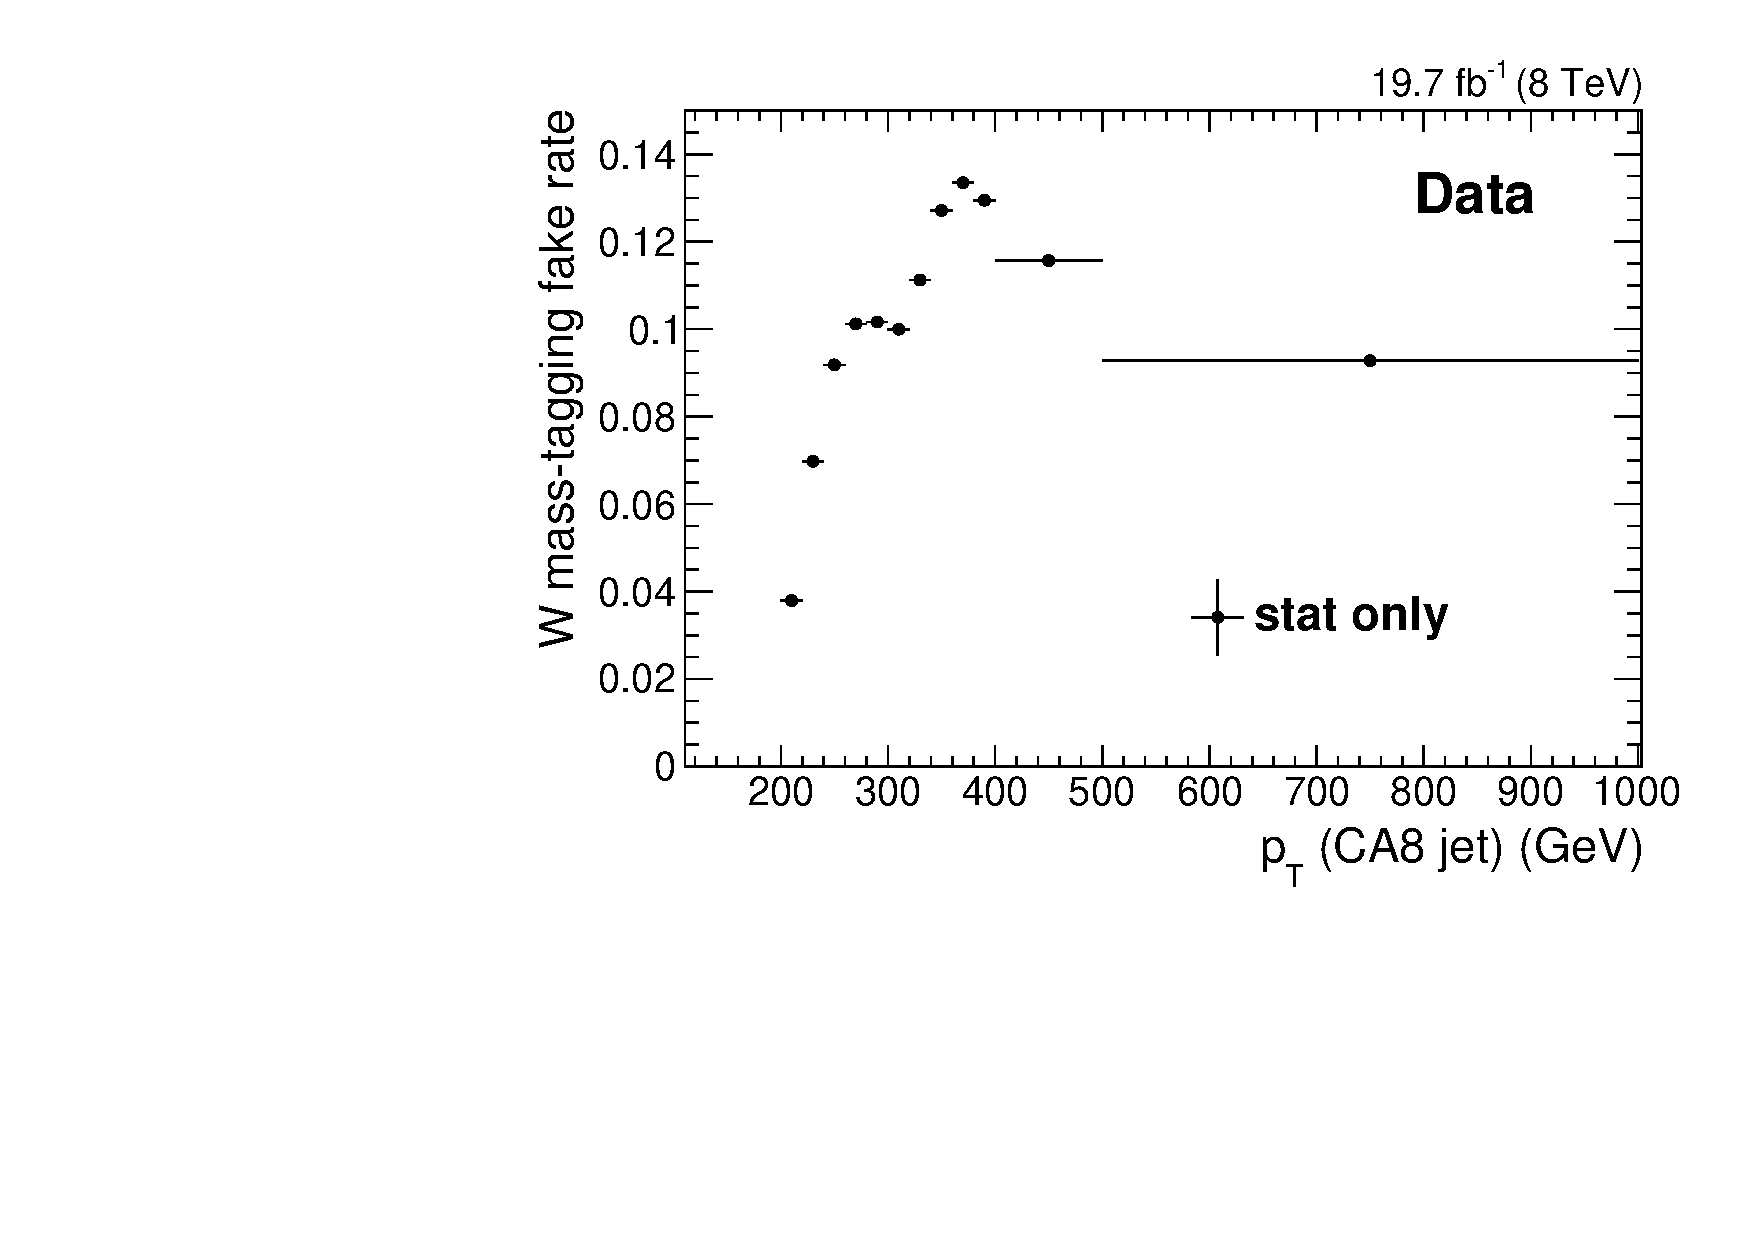
\includegraphics[width=0.6\textwidth]{figures/razor_wtag/Eff_Data_ratio_pt_Wmass_all_Data_Thesis}

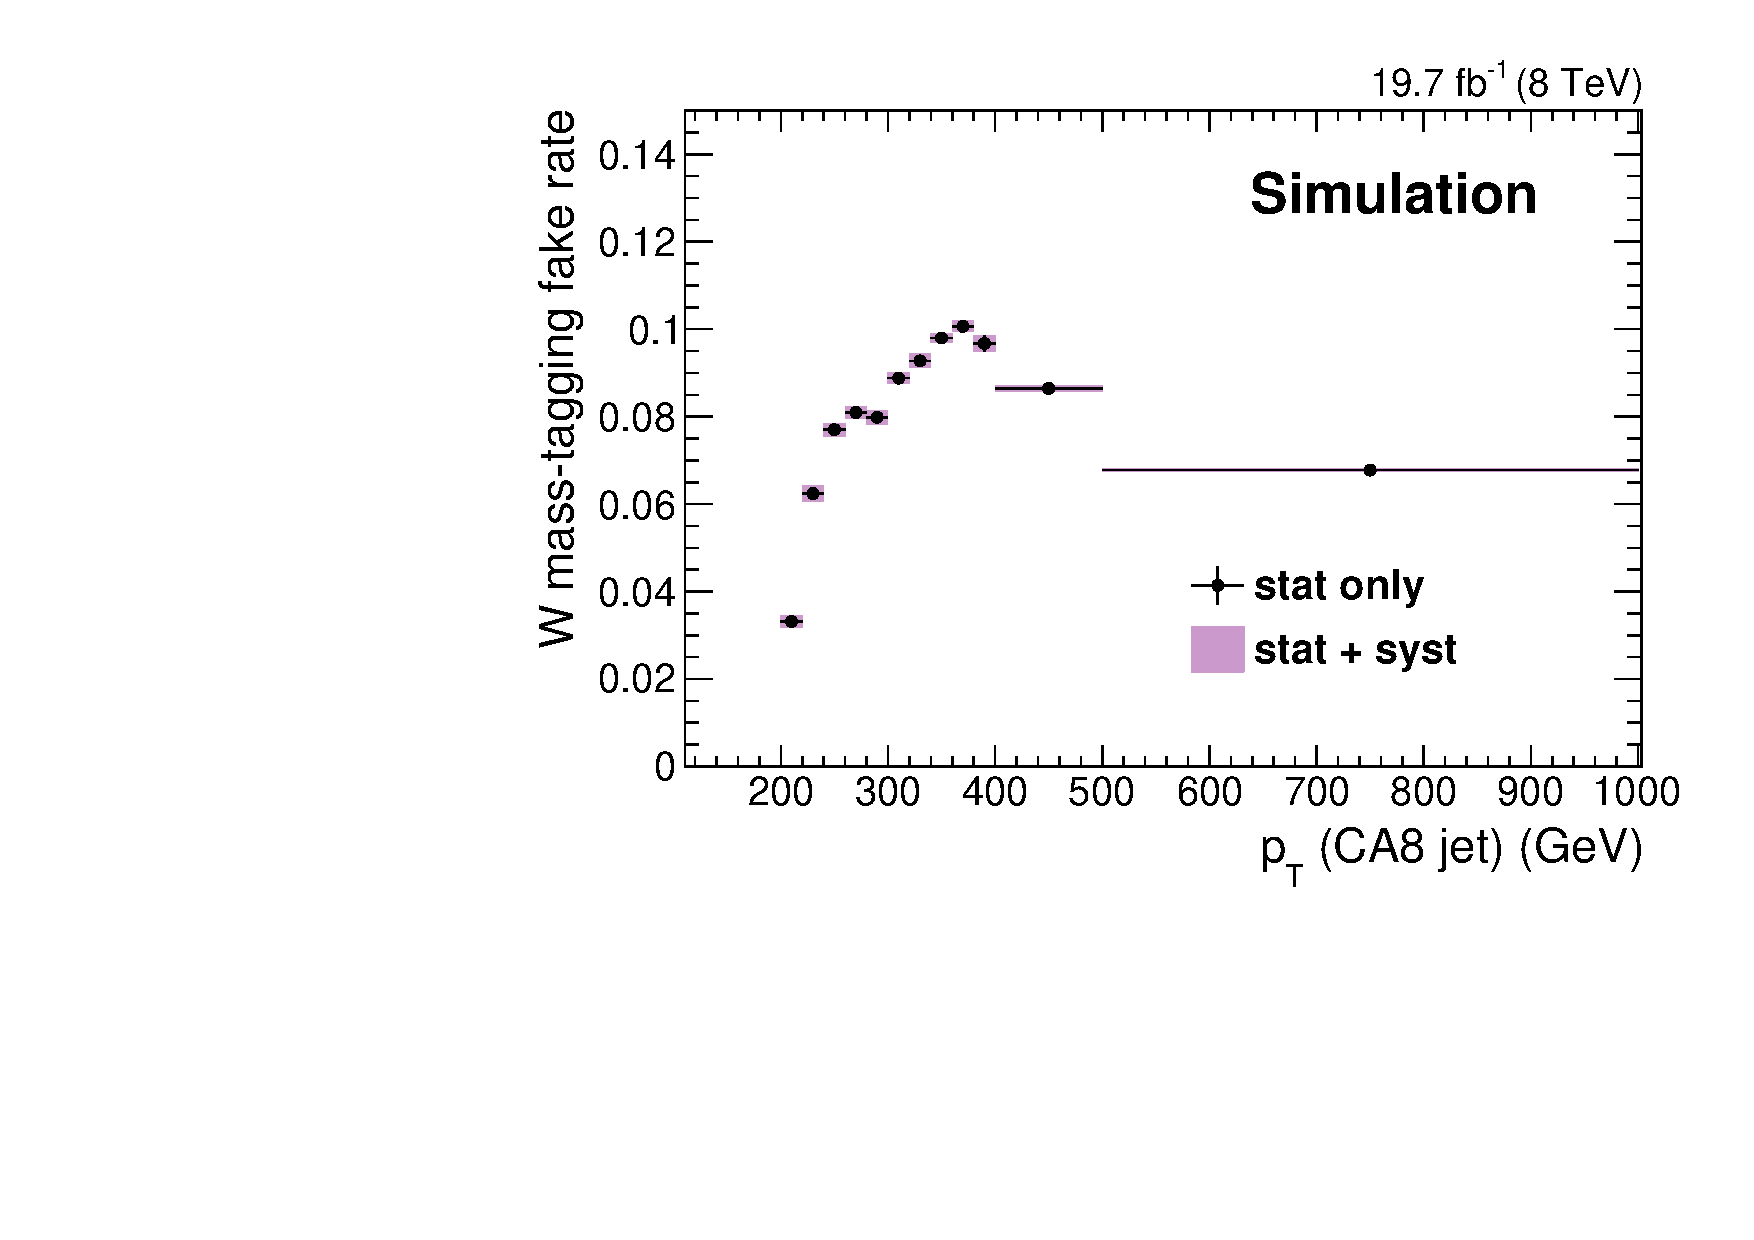
\includegraphics[width=0.6\textwidth]{figures/razor_wtag/Eff_MC_ratio_pt_Wmass_all_MC_Thesis}

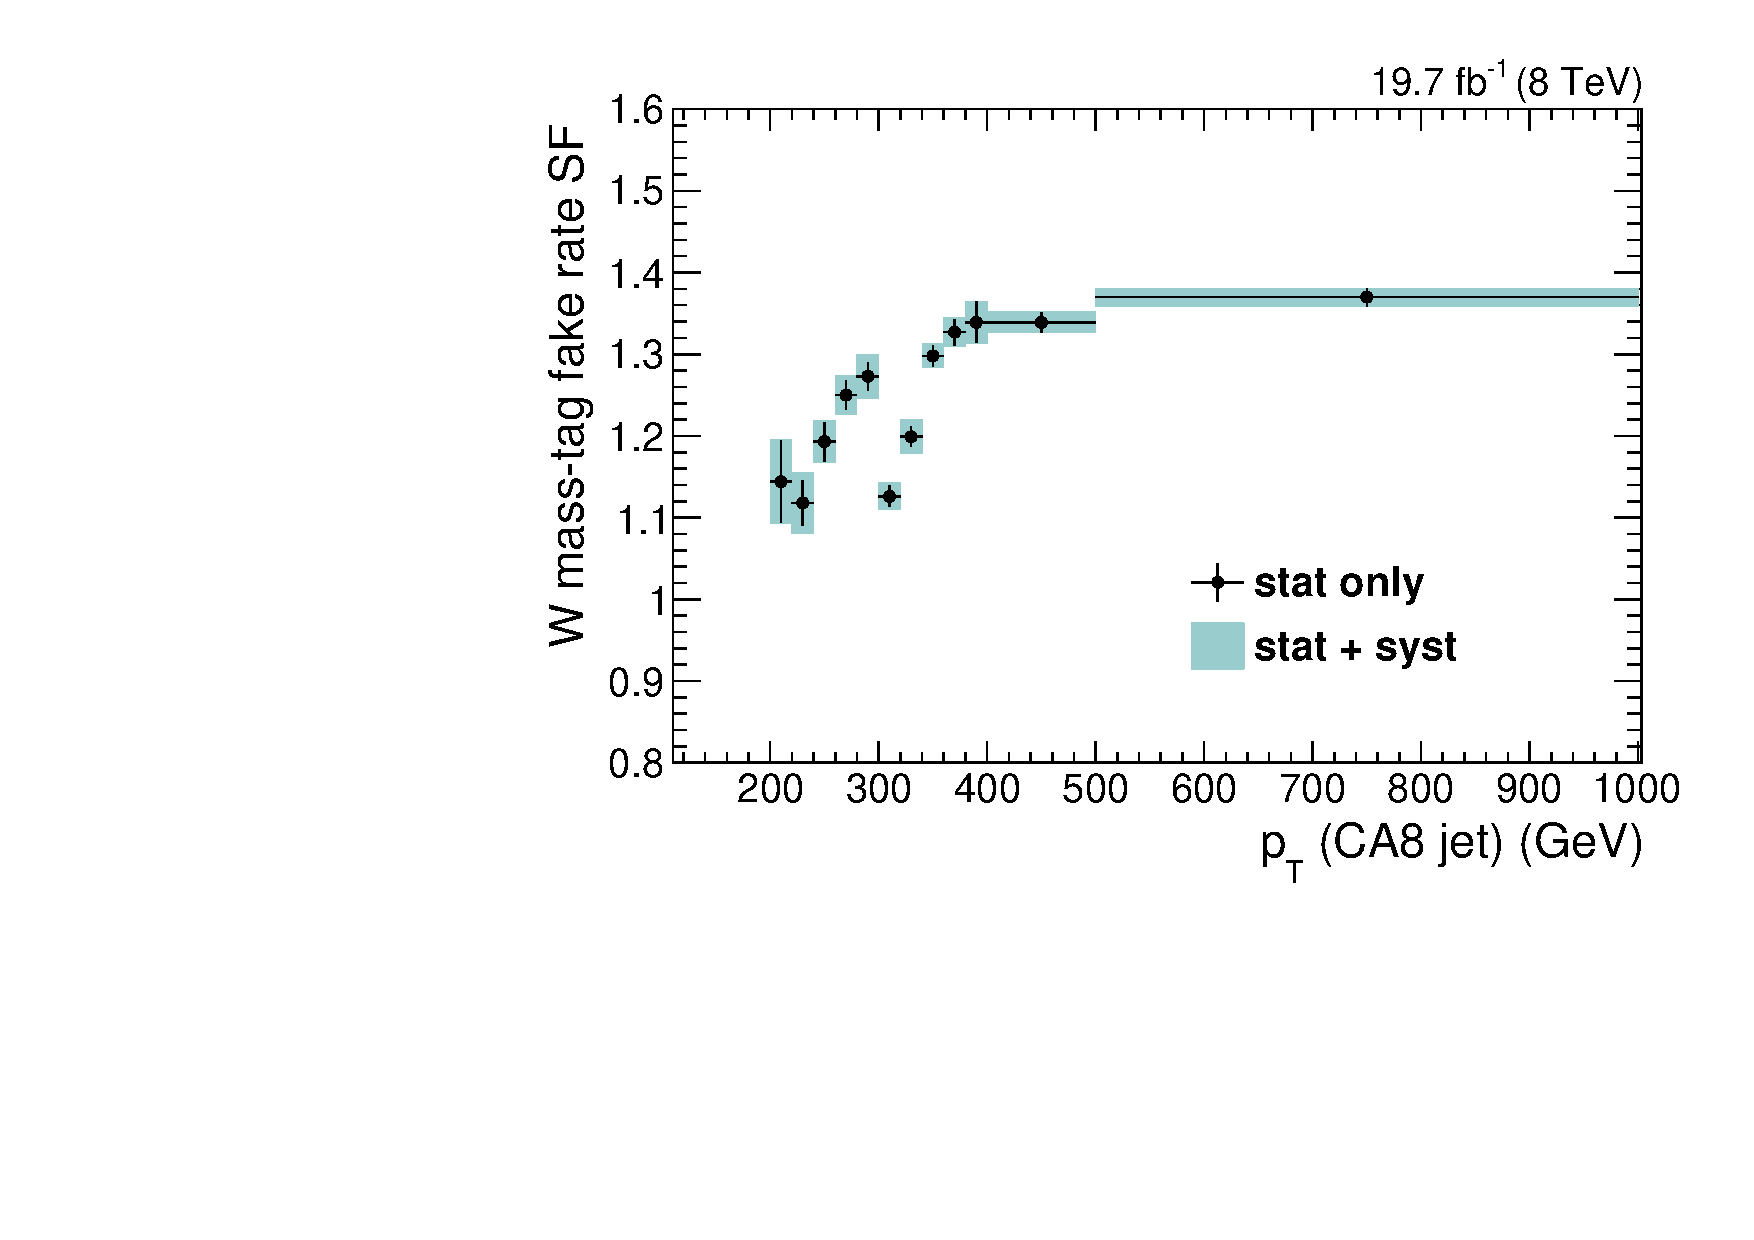
\includegraphics[width=0.6\textwidth]{figures/razor_wtag/SF_Wmass_Thesis}
\caption{[top] Misidentification probability according to $\W$ mass-tagging for a CA8 jet versus
jet \pt obtained from a multijet-enriched control region in data as described in the text. The shown
uncertainties are statistical only.
[middle] $\W$ boson mass-tag fake rate according to simulation. The uncertainty band includes
statistical and systematic uncertainties.
[bottom] Scale factor for $\W$ mass-tag fake rate versus CA8 jet \pt obtained from a
multijet-enriched control region as described in the text. The uncertainty band includes
statistical and systematic uncertainties.
\label{fig:boost_wmasstag}}
\end{figure}

%% ---------------------------------------------------------------------------------------------

\subsubsection{\texorpdfstring{$\W$}{W} boson anti-tag fake rate scale factor
\label{sec:wantitag_fake_sf}}

This scale factor corresponds to the $\W$ boson anti-tagging definition, which will be used in the
$Q$ control region. This region is dominated by QCD multijet production. Consequently, the $\W$
anti-tagged jet originates from a quark/gluon jet and is a misidentified $\W$ boson jet. Once
more, we use the same procedure and the multijet-enriched region as for the $\W$ boson tag fake
rate scale factor.

The $\W$ boson anti-tag fake rate scale factor, $SF_\textrm{Wantitag}^\textrm{fake}$, will be
applied to all simulated samples in the $Q$ region. 
Figure~\ref{fig:boost_wantitag} shows the $\W$ boson anti-tag fake rate in data and
simulation, and the corresponding scale factor versus CA8 jet \pt. As before, we observe a drop in
the scale factor just above a \pt of 300\GeV. The scale factor, and breakdown of statistical and
systematic uncertainties, is listed in Table~\ref{tab:SF_Wantitagging}. The included systematic
uncertainties are those stemming from the trigger efficiency and jet energy scale corrections. 


\begin{table}[htbp]
\centering
\caption{$\W$ boson anti-tag fake rate scale factor, binned in $\pt$. The uncertainties are broken
down in their statistical and systematic component. \label{tab:SF_Wantitagging}}
\vspace{1ex}
\begin{tabular}{c c}
\toprule
CA8 jet \pt $(\GeV)$ & $SF_{\W \textrm{antitag}}^\textrm{fake}$ \\
\midrule
$[200 - 220[$ & $1.217 \pm 0.072 \,\textrm{(stat)} \pm 0.032 \,\textrm{(sys)}$ \\
$[220 - 240[$ & $1.186 \pm 0.037 \,\textrm{(stat)} \pm 0.046 \,\textrm{(sys)}$ \\
$[240 - 260[$ & $1.216 \pm 0.033 \,\textrm{(stat)} \pm 0.011 \,\textrm{(sys)}$ \\
$[260 - 280[$ & $1.319 \pm 0.024 \,\textrm{(stat)} \pm 0.019 \,\textrm{(sys)}$ \\
$[280 - 300[$ & $1.479 \pm 0.022 \,\textrm{(stat)} \pm 0.037 \,\textrm{(sys)}$ \\
$[300 - 320[$ & $1.203 \pm 0.017 \,\textrm{(stat)} \pm 0.015 \,\textrm{(sys)}$ \\
$[320 - 340[$ & $1.244 \pm 0.016 \,\textrm{(stat)} \pm 0.026 \,\textrm{(sys)}$ \\
$[340 - 360[$ & $1.409 \pm 0.019 \,\textrm{(stat)} \pm 0.015 \,\textrm{(sys)}$ \\
$[360 - 380[$ & $1.448 \pm 0.022 \,\textrm{(stat)} \pm 0.020 \,\textrm{(sys)}$ \\
$[380 - 400[$ & $1.472 \pm 0.033 \,\textrm{(stat)} \pm 0.014 \,\textrm{(sys)}$ \\
$[400 - 500[$ & $1.487 \pm 0.017 \,\textrm{(stat)} \pm 0.012 \,\textrm{(sys)}$ \\
$[500 - ...]$ & $1.505 \pm 0.014 \,\textrm{(stat)} \pm 0.004 \,\textrm{(sys)}$ \\
\bottomrule
\end{tabular}
\end{table}


\begin{figure}[htbp]
\centering
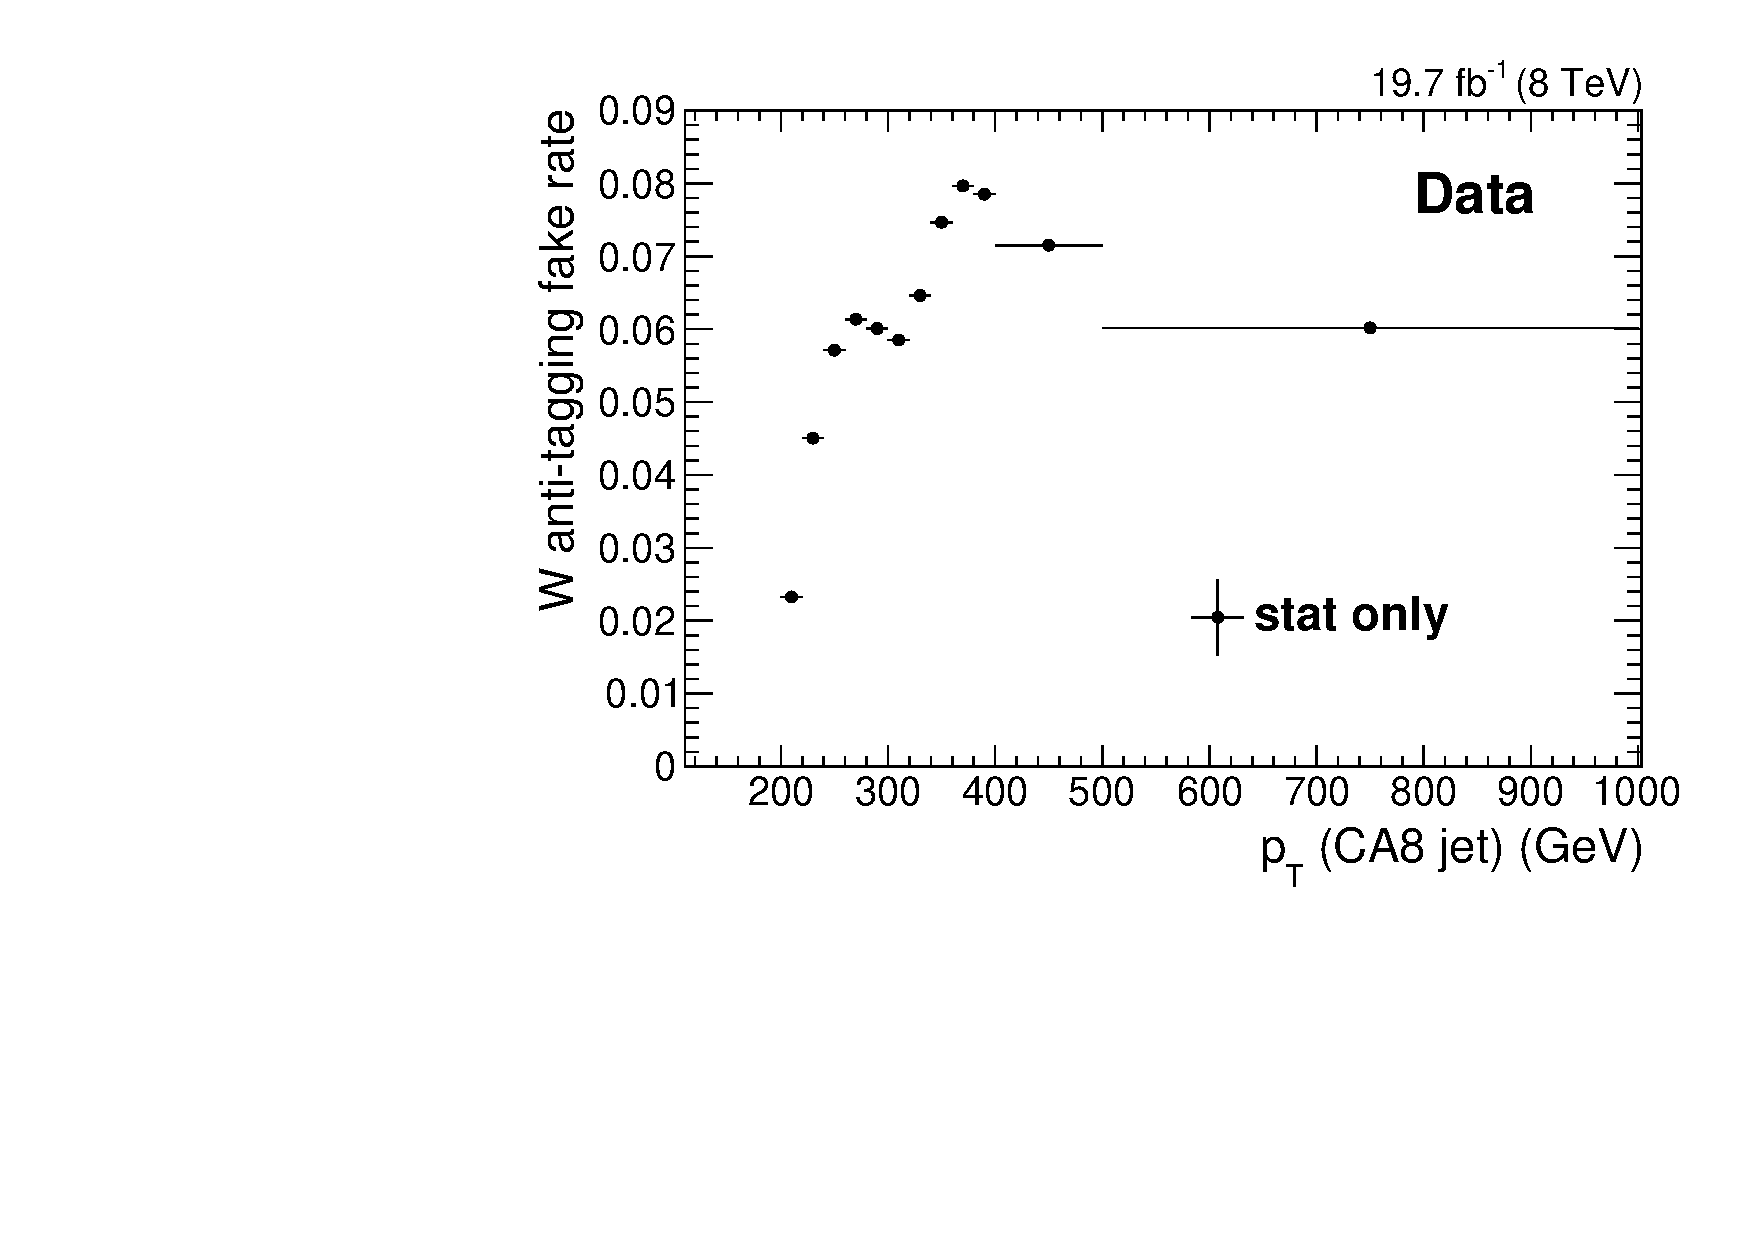
\includegraphics[width=0.6\textwidth]
{figures/razor_wtag/Eff_Data_ratio_pt_antitagged_all_Data_Thesis}

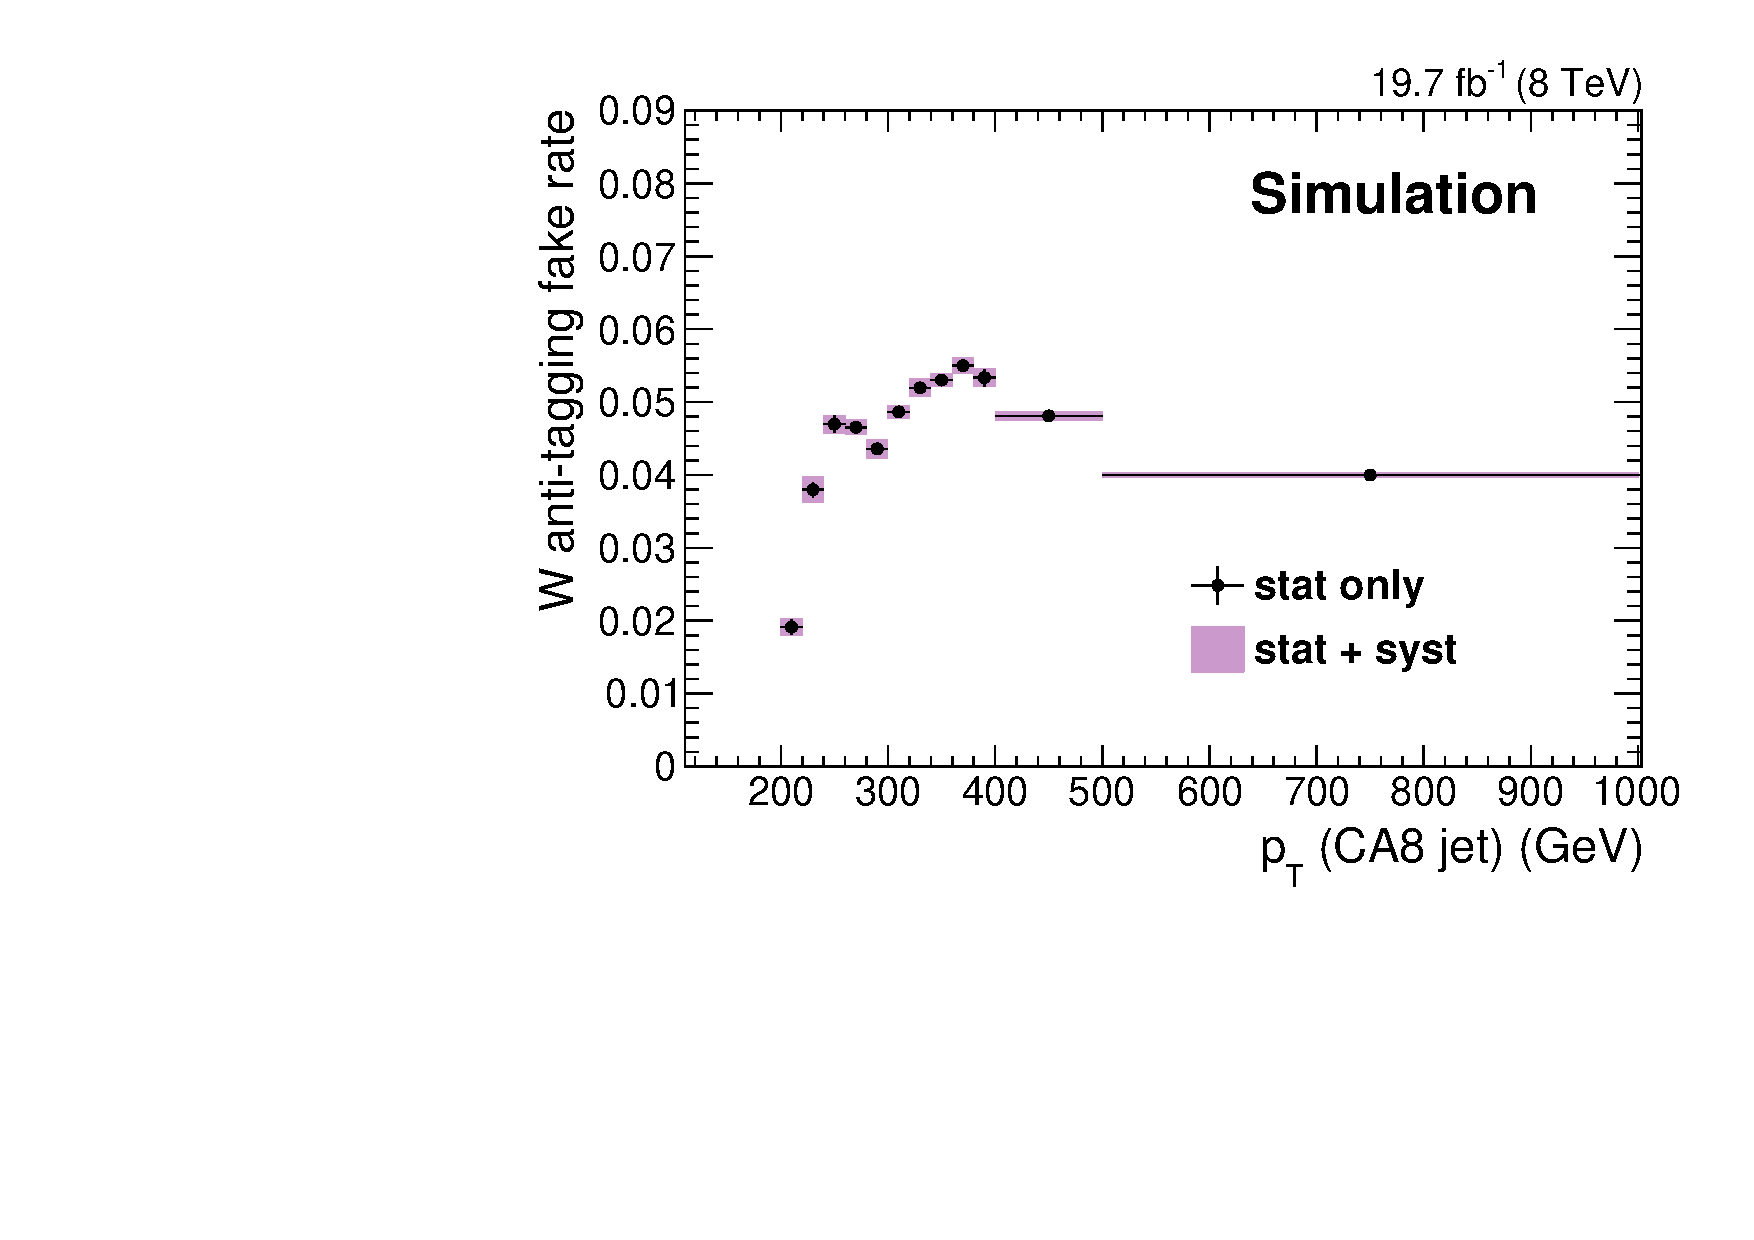
\includegraphics[width=0.6\textwidth]{figures/razor_wtag/Eff_MC_ratio_pt_antitagged_all_MC_Thesis}

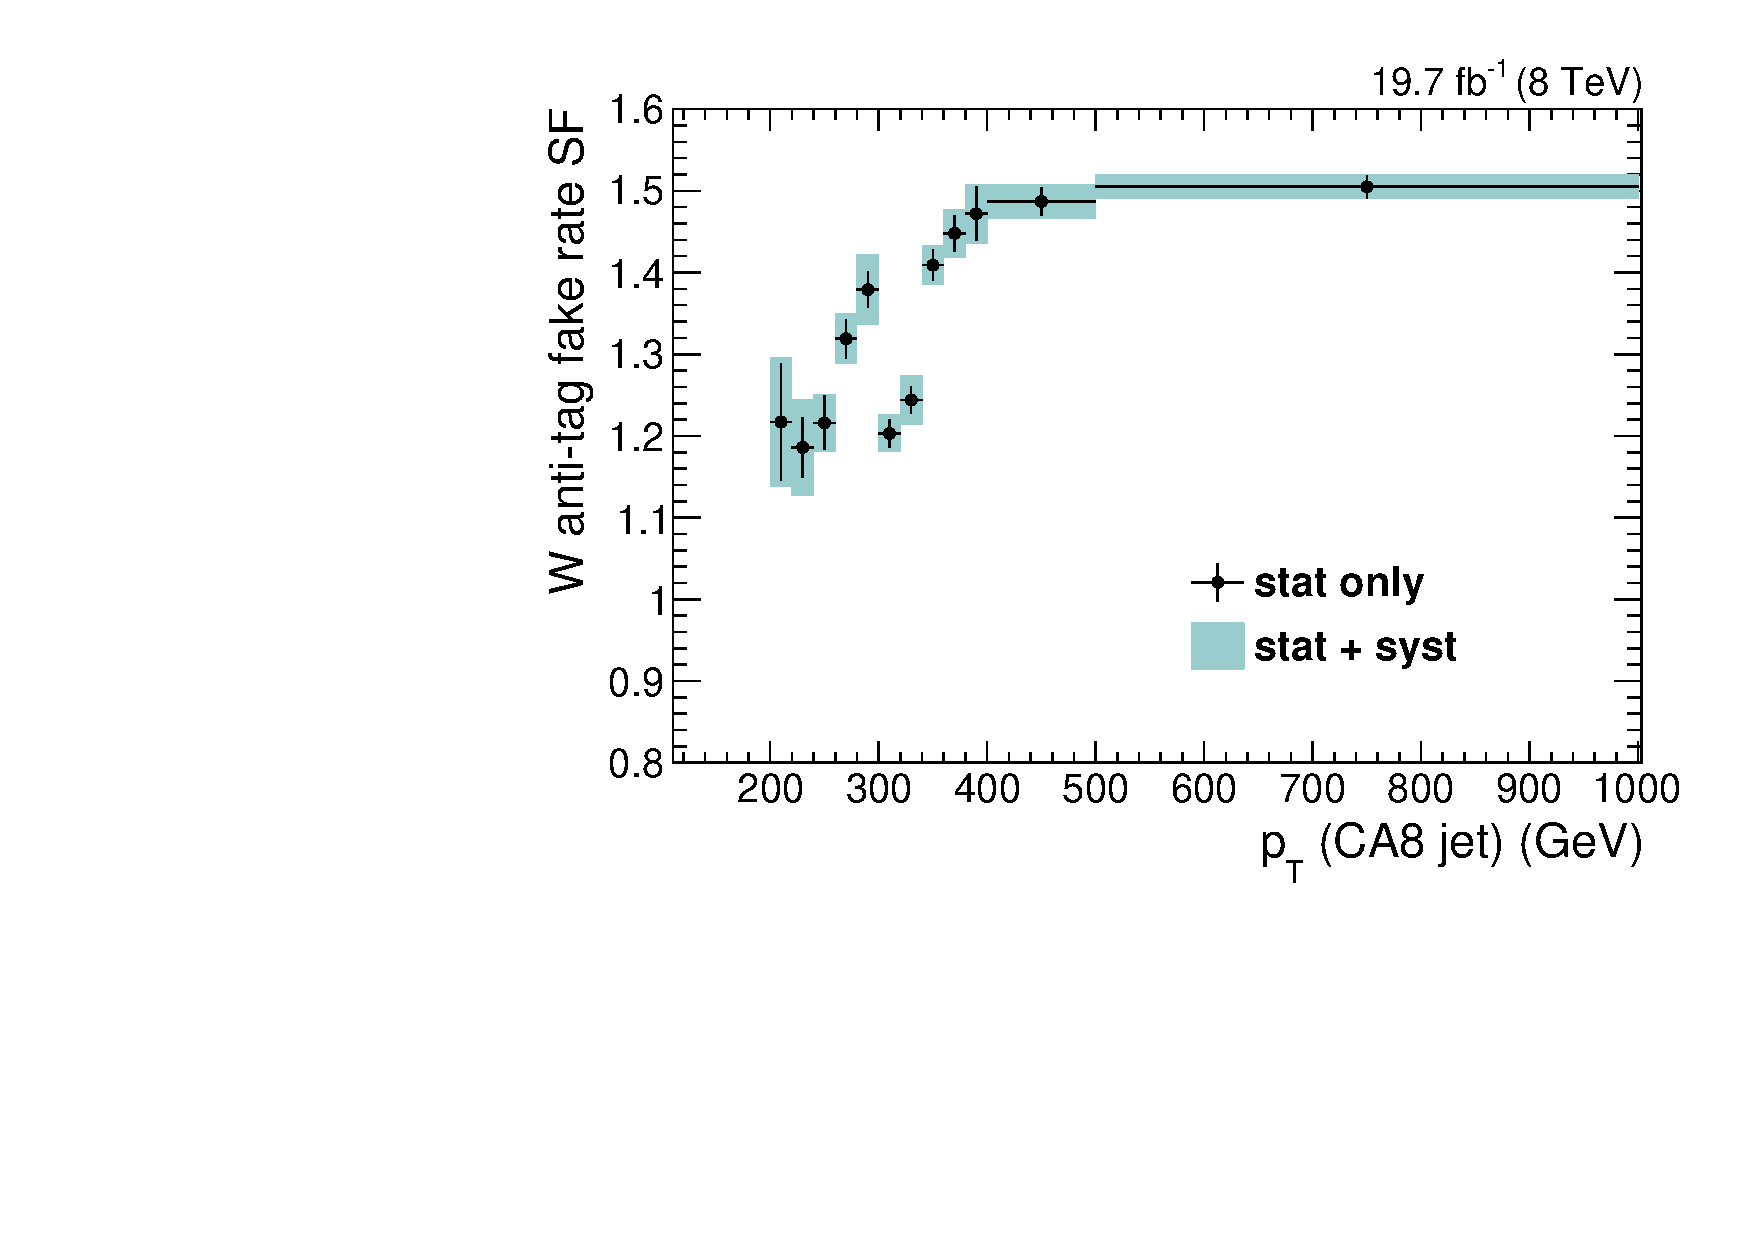
\includegraphics[width=0.6\textwidth]{figures/razor_wtag/SF_Wantitagged_Thesis}
\caption{[top] Misidentification probability according to $\W$ anti-tagging for a CA8 jet versus jet
\pt obtained from a multijet-enriched control region in data as described in the text. The shown
uncertainties are statistical only.
[middle] $\W$ boson anti-tag fake rate according to simulation. The uncertainty band includes
statistical and systematic uncertainties. 
[bottom] Scale factor for $\W$ anti-tag fake rate versus CA8 jet \pt obtained from a
multijet-enriched control region as described in the text. The uncertainty band includes
statistical and systematic uncertainties.
\label{fig:boost_wantitag}}
\end{figure}


% TODO explain the wiggle

%%%%%%%%%%%%%%%%%%%%%%%%%%%%%%%%%%%%%%%%%%%%%%%%%%%%%%%%%%%%%%%%%%%%%%%%%%%%%%%%%%%%%%%%%%%%%%%%%%%%



% 
% As we can see from these figures, there is a drop in the scale factor around a \pt of 300\GeV. 
% This is a result of a residual mismodeling of the trigger efficiency, as is explained in more detail
% in appendix~\ref{app:wiggle}. 
% Given that we understand the origin of this wiggle, we decide to keep the binning quite fine in that
% region, so that we can correct for the effect. 

\begin{table}[htbp]
\centering
\caption{Summary of scale factors and their total uncertainty. \label{tab:SF_summary}}
\vspace{1ex}
\begin{tabular}{c c c c}
\toprule
CA8 jet \pt (\GeV) & $SF_{\W\textrm{tag}}^\textrm{fake}$ & $SF_{\W \textrm{masstag}}^\textrm{fake}$
& $SF_{\W\textrm{antitag}}^\textrm{fake}$ \\
\midrule
$[200 - 220[$ & $1.04 \pm 0.07$ & $1.14 \pm 0.06$ & $1.22 \pm 0.08$ \\
$[220 - 240[$ & $1.01 \pm 0.04$ & $1.12 \pm 0.04$ & $1.19 \pm 0.06$ \\
$[240 - 260[$ & $1.16 \pm 0.04$ & $1.19 \pm 0.03$ & $1.22 \pm 0.04$ \\
$[260 - 280[$ & $1.16 \pm 0.03$ & $1.25 \pm 0.03$ & $1.32 \pm 0.04$ \\
$[280 - 300[$ & $1.15 \pm 0.03$ & $1.27 \pm 0.03$ & $1.38 \pm 0.05$ \\
$[300 - 320[$ & $1.03 \pm 0.02$ & $1.13 \pm 0.02$ & $1.20 \pm 0.03$ \\
$[320 - 340[$ & $1.14 \pm 0.02$ & $1.20 \pm 0.03$ & $1.24 \pm 0.03$ \\
$[340 - 360[$ & $1.17 \pm 0.02$ & $1.30 \pm 0.02$ & $1.41 \pm 0.03$ \\
$[360 - 380[$ & $1.18 \pm 0.03$ & $1.33 \pm 0.02$ & $1.45 \pm 0.03$ \\
$[380 - 400[$ & $1.18 \pm 0.03$ & $1.34 \pm 0.03$ & $1.47 \pm 0.04$ \\
$[400 - 500[$ & $1.15 \pm 0.02$ & $1.34 \pm 0.02$ & $1.49 \pm 0.03$ \\
$[500 - ...]$ & $1.18 \pm 0.02$ & $1.37 \pm 0.02$ & $1.51 \pm 0.02$ \\
\bottomrule
\end{tabular}
\end{table}






\section{Trigger and datasets \label{sec:trigger_datasets}}

%%%%%%%%%%%%%%%%%%%%%%%
% trigger and datasets 
%%%%%%%%%%%%%%%%%%%%%%%

\subsection{Data and trigger \label{sec:boost_data_trigger}}

The analysis presented in this thesis is based on 19.7\fbinv of 8\TeV proton-proton collision data
collected by the CMS experiment in 2012.  The data are divided into four data taking periods
(A, B, C, and D) to deal with changing conditions such as the average pileup or peak luminosity. 
Events used in the razor boost analysis are selected using two triggers from the CMS high
level trigger system (see Section~\ref{sec:cms_hlt}), requiring either the highest jet \pt or the
scalar sum of jet transverse momenta, $\HT$, to be above certain thresholds. 
The jet \pt trigger, of which the different implementations are denoted by \texttt{PFJet*},
had a threshold on the \pt of the highest \pt jet of 320\GeV for most of the runs, and a threshold
of 400\GeV for a short period. 
The $\HT$-based trigger, denoted by \texttt{PFHT*}, had an $\HT$ threshold of 650\GeV. 
The two trigger algorithms were based on a fast implementation of the particle flow 
reconstruction method, which was described in Section~\ref{sec:event_reco_pf}.  
The exact names of the trigger used by run are given in Table~\ref{tab:boost_triggers}. The primary
datasets which include the data collected by these triggers are listed in
Table~\ref{tab:boost_primary_datasets}. 

\begin{table}[htdp]
\caption{Summary of HLT triggers that are used in this analysis. Events in a given run range
are selected if they pass at least one of the listed triggers. }	
\begin{center}
\begin{tabular}{l l l l}
\toprule
Period & Run range & PFJet HLT & PFHT HLT \\
\midrule
\multirow{3}{*}{Run2012A} & 190456 - 190738 & PFJet320\_v3 & PFHT650\_v5 \\
& 190762 - 191426 & PFJet320\_v4 & PFHT650\_v6 \\
& 191512 - 193686 & PFJet320\_v5 & PFHT650\_v7 \\
\midrule
\multirow{2}{*}{Run2012B} & 193746 - 196027 & PFJet320\_v5 & PFHT650\_v8 \\
& 196039 - 197722 & PFJet320\_v5 & PFHT650\_v9 \\
\midrule
\multirow{3}{*}{Run2012C} & 197770 - 199631 & PFJet400\_v6 & PFNoPUHT650\_v1 \\
& 199648 - 202585 & PFJet320\_v8 & PFNoPUHT650\_v3 \\
& 202807 - 203734 & PFJet320\_v9 & PFNoPUHT650\_v4 \\
\midrule
Run2012D & 203754 - 208940 & PFJet320\_v9 & PFNoPUHT650\_v4 \\
\bottomrule
\end{tabular}
\end{center}
\label{tab:boost_triggers}
\end{table}

\begin{table}[htdp]
\caption{List of primary datasets and corresponding run ranges, containing data for a total
integrated luminosity of $19.712\fbinv$.}
\begin{center}
\begin{tabular}{ l l }
\toprule
Primary dataset & Run range \\
\midrule
/Jet/Run2012A-22Jan2013-v1/ & 190456 - 193621 \\
/HT/Run2012A-22Jan2013-v1/  & 190456 - 193621 \\
/JetHT/Run2012B-22Jan2013-v1/ & 193833 - 196531 \\
/JetHT/Run2012C-22Jan2013-v1/ & 198022 - 203742 \\
/JetHT/Run2012D-22Jan2013-v1/ & 203777 - 208686  \\
\bottomrule
\end{tabular}
\end{center}
\label{tab:boost_primary_datasets}
\end{table}

\begin{table}[htdp]
\caption{List of primary datasets used to measure the trigger efficiency. }
\begin{center}
\begin{tabular}{ l l }
\toprule
Primary dataset & Run range \\
\midrule
/SingleElectron/Run2012A-22Jan2013-v1/ & 190456 - 193621 \\ 
/SingleElectron/Run2012B-22Jan2013-v1/ & 193833 - 196531 \\
/SingleElectron/Run2012C-22Jan2013-v1/ & 198022 - 203742 \\
/SingleElectron/Run2012D-22Jan2013-v1/ & 203777 - 208686  \\
\midrule
/SingleMu/Run2012A-22Jan2013-v1/ & 190456 - 193621 \\ 
/SingleMu/Run2012B-22Jan2013-v1/ & 193833 - 196531 \\
/SingleMu/Run2012C-22Jan2013-v1/ & 198022 - 203742 \\
/SingleMu/Run2012D-22Jan2013-v1/ & 203777 - 208686 \\
\bottomrule
\end{tabular}
\end{center}
\label{tab:boost_primary_datasets_trigeff}
\end{table}

In order to select events with unbiased jet \pt and $\HT$ distributions,
the trigger efficiency was measured from a sample of events collected with an orthogonal set of
triggers requiring at least one electron or muon. The corresponding primary datasets are listed in
Table~\ref{tab:boost_primary_datasets_trigeff}. 
The trigger efficiency $\epsilon_\textrm{trig}$ is determined as a function of $\HT$ and first jet
\pt, and takes as basis for the measurement the baseline selection described further in
Section~\ref{sec:boost_baseline_selection},
\begin{equation}
  \epsilon_\textrm{trig} = \frac{\textrm{Events passing baseline and trigger selection}}
{\textrm{Events passing baseline selection}}.
\end{equation}
It was checked that the trigger efficiency obtained from either the electron or muon sample gives 
consistent results. Both samples were combined to derive the final trigger efficiency measurement in 
order to increase the statistical precision.
Figure~\ref{fig:boost_trigger_efficiency} shows, on the top plot, the trigger efficiency
measured from data on the ($\HT$, first jet \pt) plane.
We observe that the trigger is fully efficient for events with $\HT > 800\GeV$.  
In order to account for the lower efficiency of the region with $\HT  < 800\GeV$, the measured
trigger efficiency over the ($\HT$, first jet \pt) plane is applied as an event-by-event weight
to the simulated samples. The bottom plot of Fig.~\ref{fig:boost_trigger_efficiency} shows the
effect of this trigger efficiency across the (\mr,\rsq) plane for the total simulated background. 
The uncertainty in the trigger efficiency is taken to be the maximum of the statistical 
uncertainty, and the difference in trigger efficiency obtained using the baseline selection and no 
selection at all. As the uncertainties are not symmetric, we show both the up and down uncertainties
in Fig.~\ref{fig:boost_trigger_efficiency_unc}. They are generally below 5\%.   


\begin{figure}[p]
\centering
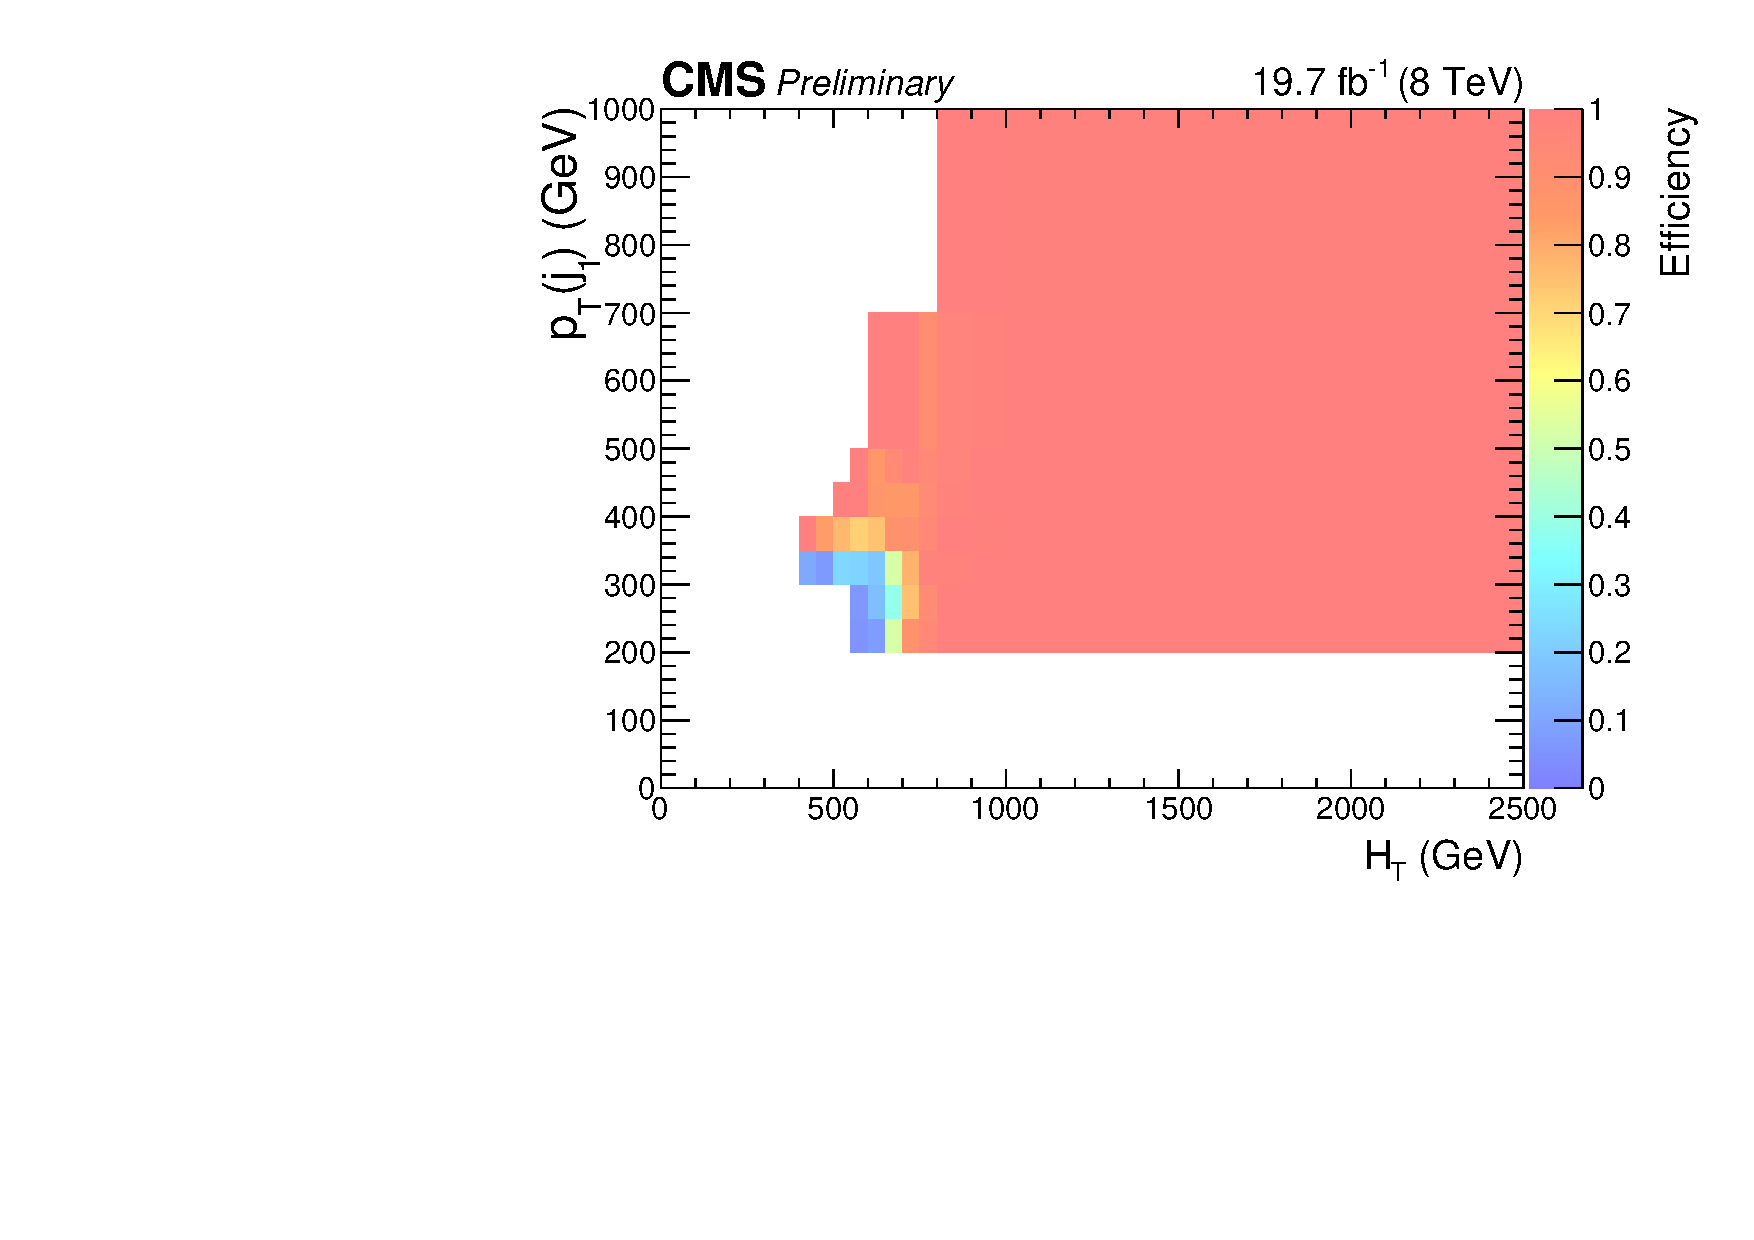
\includegraphics[width=0.9\textwidth]{figures/razor_trigger/h_HT_j1pt_pre_eff_ph_l}

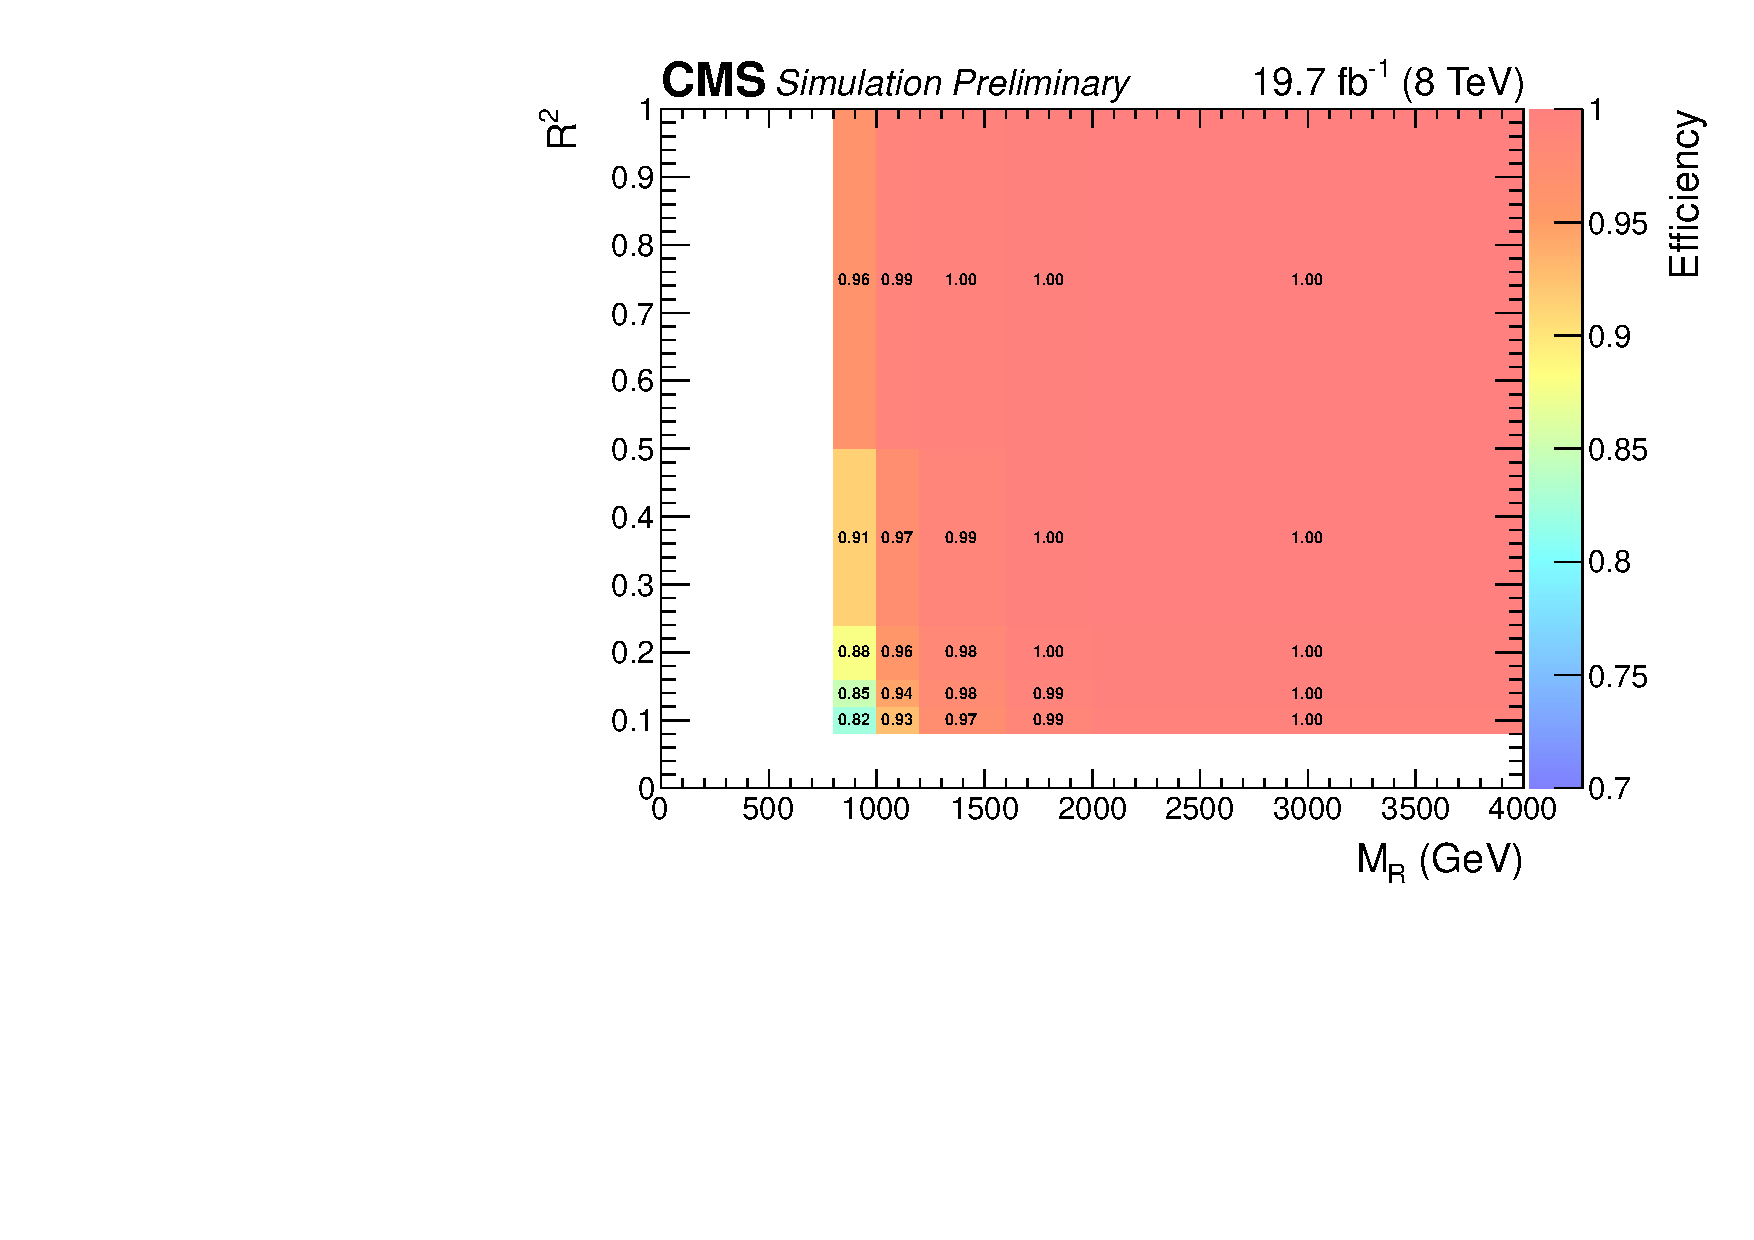
\includegraphics[width=0.9\textwidth]{figures/razor_trigger/MR_R2_bg_trig_eff}
\caption{[top] The trigger efficiency, obtained from data, as a function of $H_T$ and first jet
$\pt$ after the preselection mentioned in Section~\ref{sec:boost_baseline_selection}.
[bottom] The trigger efficiency as a function of $\mathrm{M_R}$ and $\mathrm{R^2}$ after the same
preselection, obtained by applying the trigger efficiency as a function of $\HT$ and first jet $\pt$
to the total simulated background. 
\label{fig:boost_trigger_efficiency}}
\end{figure}  

\begin{figure}[htpb]
\centering
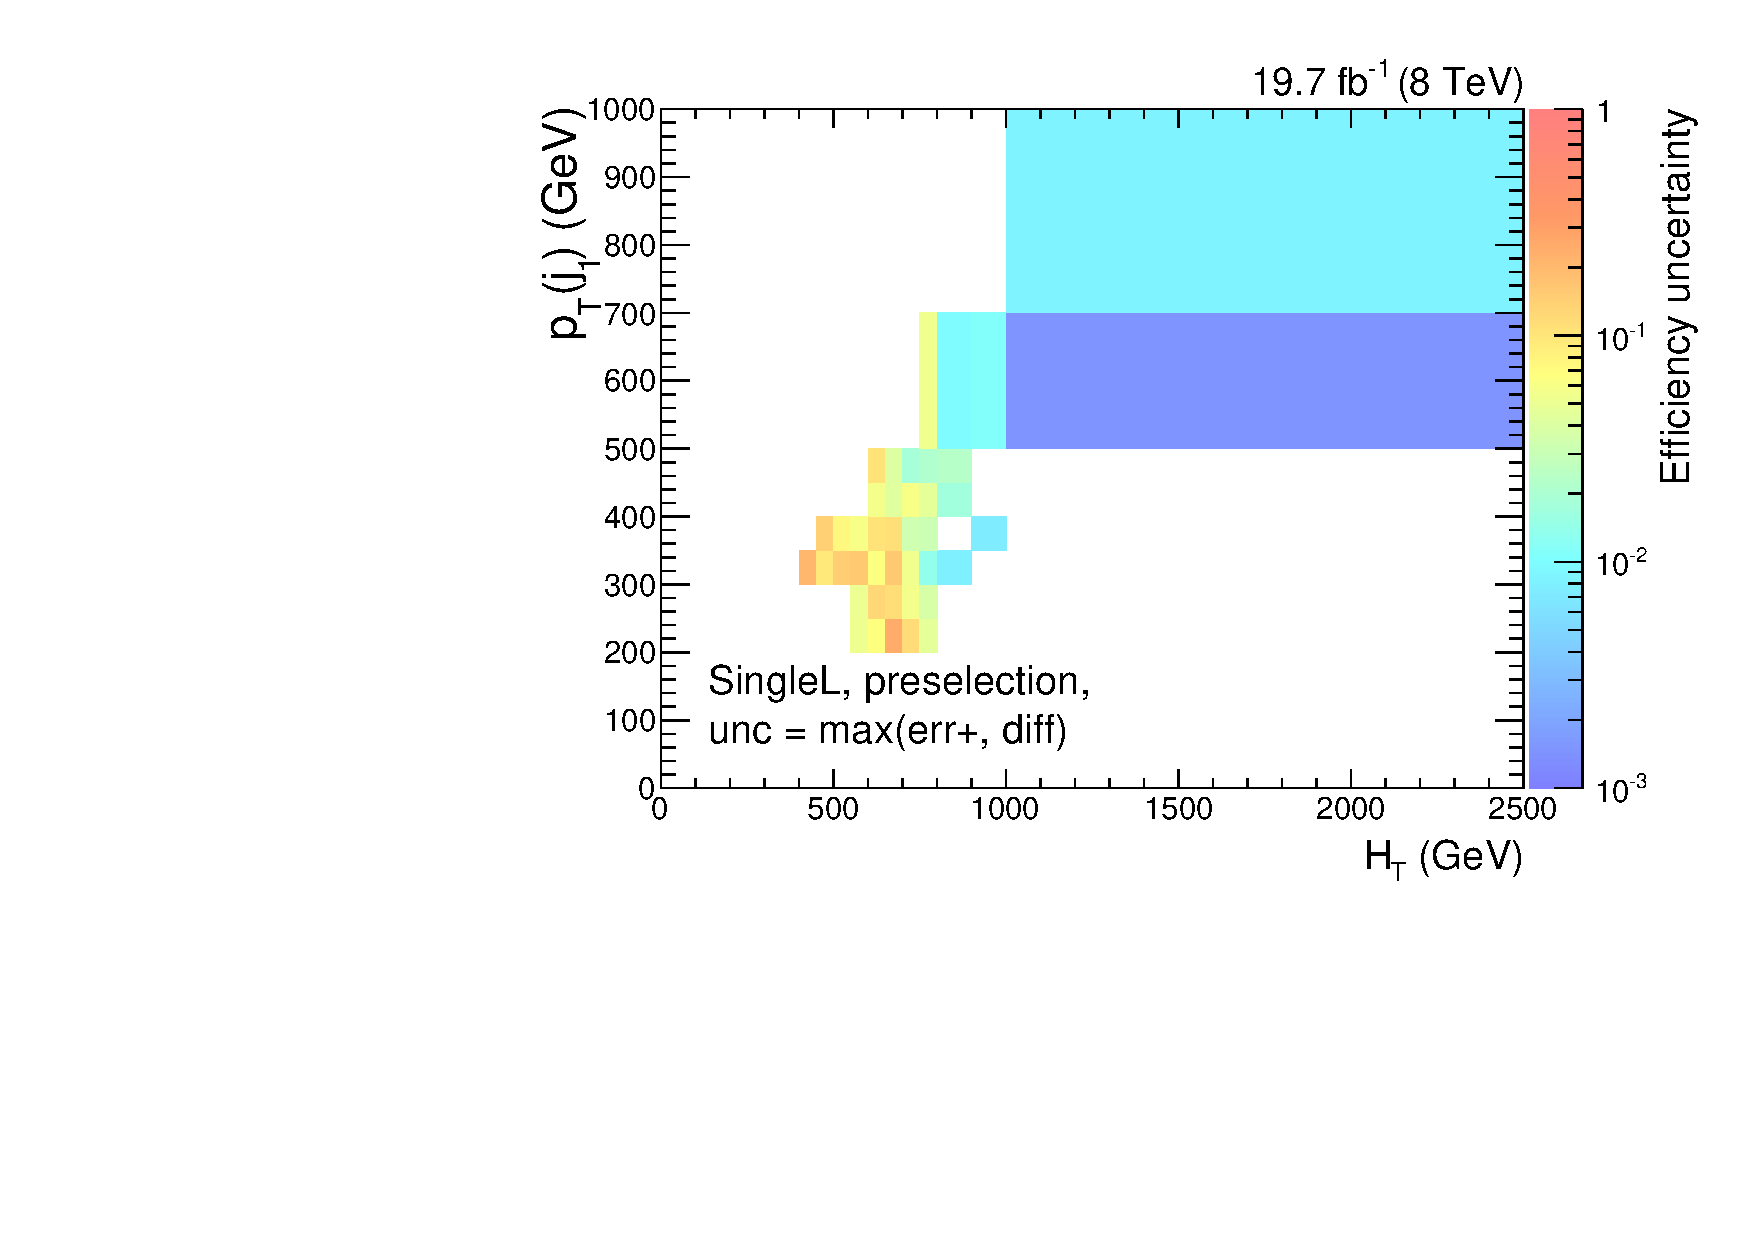
\includegraphics[width=0.48\textwidth]
{figures/razor_trigger/h_HT_j1pt_0_pre_errdiff_up_ph_l_forThesis}
~
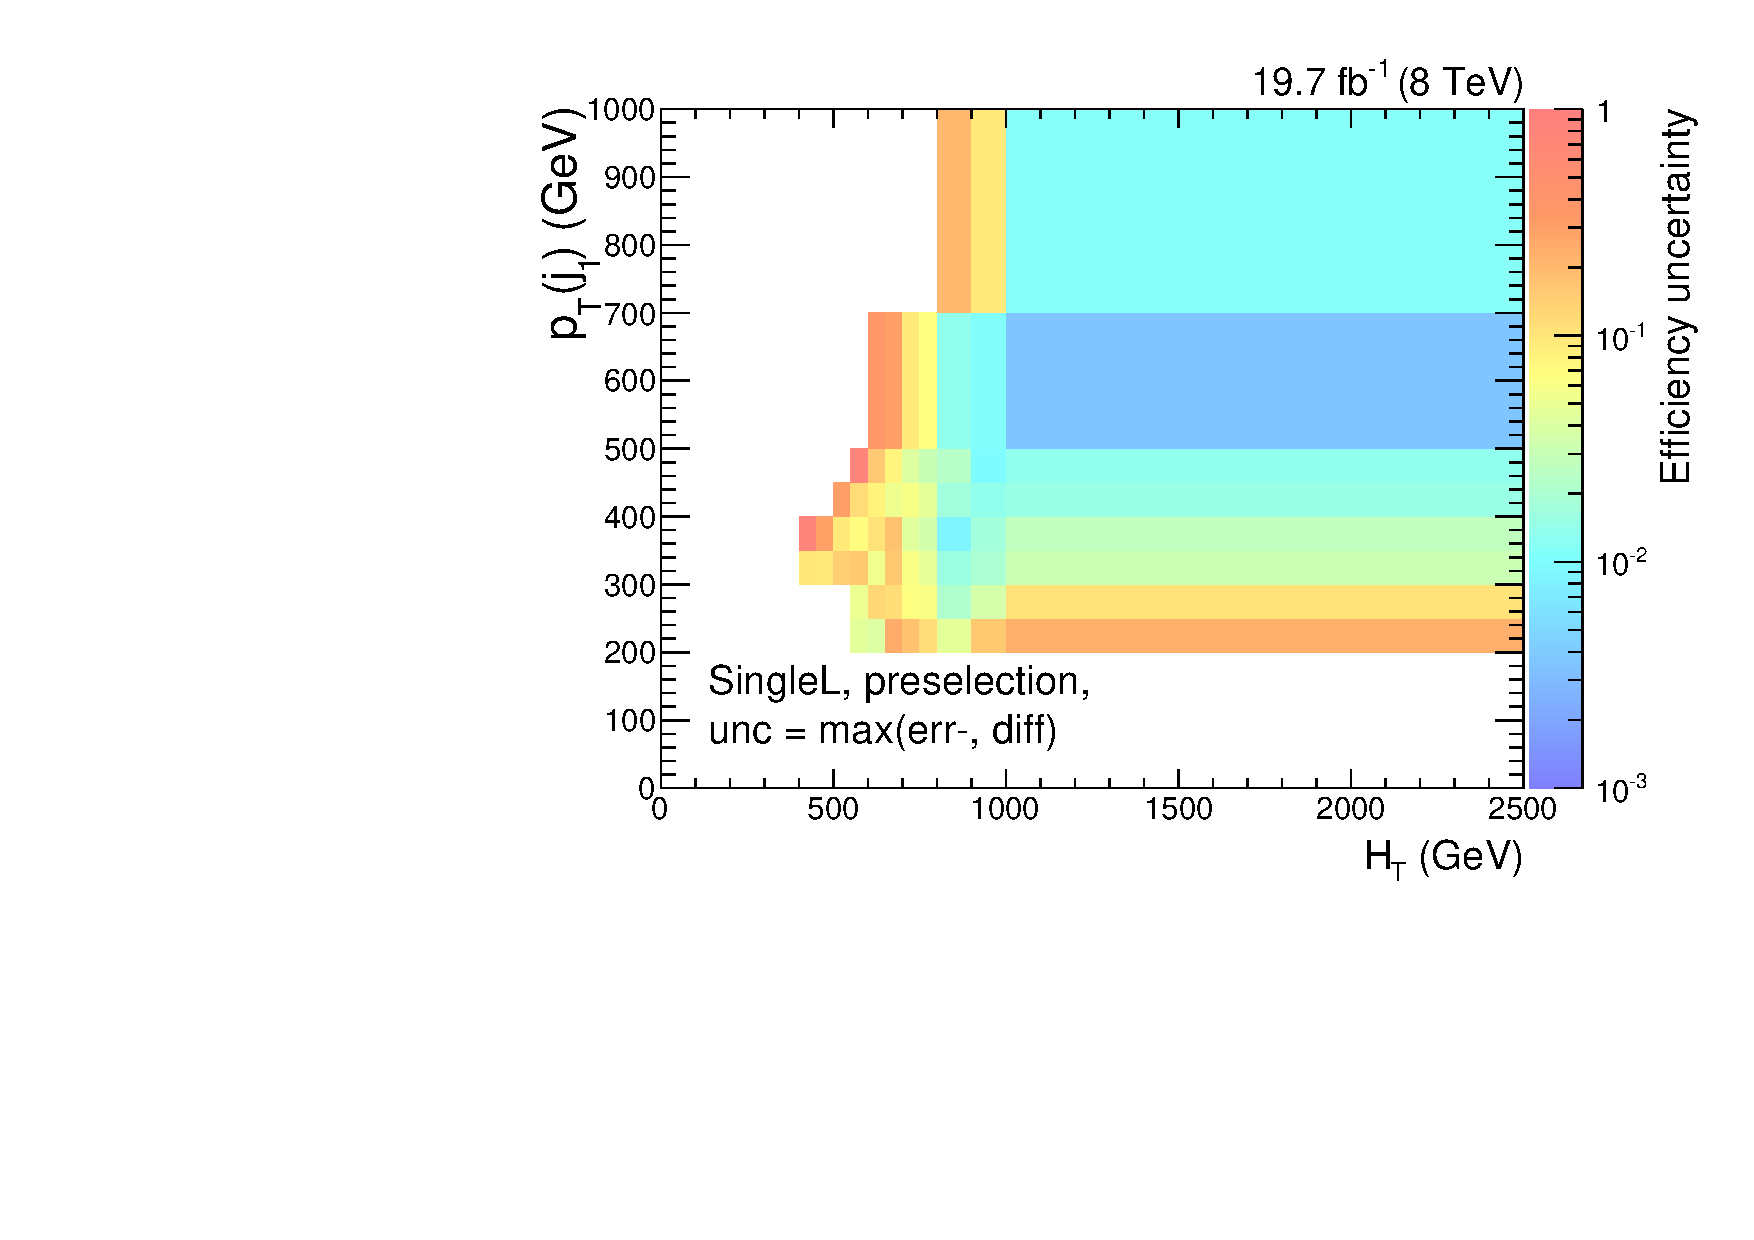
\includegraphics[width=0.48\textwidth]
{figures/razor_trigger/h_HT_j1pt_0_pre_errdiff_low_ph_l_forThesis}
\caption{The magnitude of the up (left) and down (right) uncertainties on the efficiency as 
functions of $\HT$ and first jet $\pt$, obtained using the combination of the SingleEle and SingleMu 
datasets. 
\label{fig:boost_trigger_efficiency_unc}}
\end{figure}



%%%%%%%%%%%%%%%%%%%%%%%%%%%%%%%%%%%%%%%%%%%%%%%%%%%%%%%%%%%%%%%%%%%%%%%%%%%%%%%%%%%%%%%%%%%%%%%%%%%%
\subsection{Simulated samples \label{sec:boost_mc_samples}}

The simulated samples are used to investigate the characteristics of the background and signal
processes.  The complete list of simulated samples that are used in the analysis is given in
Appendix~\ref{app:datasets}, in Tables~\ref{tab:boost_mc_bg} and \ref{tab:boost_mc_bg2} for the SM
background samples, and in Table~\ref{tab:boost_mc_sms} for the signal samples. 

Multijet, $t\bar{t}$, $\W({\rightarrow}\,\ell\nu)+$jets, $\cPZ/\gamma^*({\rightarrow}\,
\ell\bar{\ell})+$jets, and $\cPZ({\rightarrow}\, \nu \bar{\nu})+$jets events are generated using
\MADGRAPH 5.1.3.30~\cite{Alwall:2011uj}, as are the smaller backgrounds $\W({\rightarrow}\, q
\bar{q})bb$, 
$\W\W\cPZ+$jets, $\W\W\gamma+$jets, $\cPZ\cPZ\cPZ+$jets, $t\bar{t}\gamma+$jets, and
$t\bar{t}\W\W+$jets.
Events for the $\cPZ/\gamma^*({\rightarrow} c\bar{c})$, $\cPZ/\gamma^*({\rightarrow}
\cPqb\bar{\cPqb})$,
$\W\W$, $\W\cPZ$, and $\cPZ\cPZ$ processes are generated using 
{\PYTHIA}6.424~\cite{Sjostrand:2006za}.
For all these samples CTEQ6L1~\cite{Pumplin:2002vw} is used as the set of parton distribution
functions. 
Single top quark events are generated using \POWHEG 1.0~\cite{powheg,powheg2} with CT10
PDFs~\cite{Lai:2010vv}, and $\W\W\W$, $\W\cPZ\cPZ$, $t\bar{t}\W$ and $t\bar{t}\cPZ$ are generated using
\AMCATNLO~\cite{Frixione:2002ik} with CTEQ6M PDFs~\cite{Pumplin:2002vw}. 
Signal events are produced using \MADGRAPH 5.1.5.4 with CTEQ6L1 PDFs.  

The parton level events are showered and hadronized using {\PYTHIA}6.426 with tune
Z2*~\cite{Chatrchyan:2013gfi}, except for the samples generated with \AMCATNLO which use 
\HERWIG~\cite{Corcella:2000bw,Corcella:2002jc} for the parton shower and hadronization.  
The \MADGRAPH samples are matched to the parton shower using the MLM technique, as discussed
in Section~\ref{sec:event_matching}.
For the background events, the response of the CMS detector is
simulated with a full simulation based on \GEANTfour~\cite{G4}.  
A parameterized fast detector simulation, \ie FastSim (Section~\ref{subsec:fastsim}), is used to
simulate the detector response to the signal events. 





\section{Event selection \label{sec:boost_event_selection}}

In this section I will discuss the event selection. I will start by detailing the baseline
selection that is applied, and then move on to the signal region selection and the definition of the
different control regions. 
An overview of those different regions, how they are related and how they are used in the
background estimation was already shown in Fig.~\ref{fig:boost_flowchart}. 

Let us remind ourselves of the goal of the analysis and the basics of the background estimation
method. 
The aim of the analysis is to conduct a search for deviations from the SM in the high $\mr$-high
$\rsq$ region using hadronic events with at least one boosted $\W$ boson and one $b$ jet.
Standard model backgrounds in the signal region are estimated via a likelihood method, using
observations in three control regions in data, labelled $Q$, $T$ and $W$, and transfer factors
$\kappa$, calculated from simulated data, between these control regions and the signal region,
$S$. 
The viability of the defined control regions to model the data in our signal region is tested by
two closure tests, which are presented at the end of this section.
For all details on the full background estimation itself, I refer to
section~\ref{sec:boost_likelihood}. 

\subsection{Baseline selection \label{sec:boost_baseline_selection}}

%%%%%%%%%%%%%%%%%%%%%%%%%
% Baseline selection
%%%%%%%%%%%%%%%%%%%%%%%%%

The baseline selection for the Razor Boost analysis is driven by the two components of its name, in
addition to requiring the event to be of good quality.
As we use the razor variables, we need to be able to compute them. This means that there should be
at least two jets in the final state. The megajets from which the razor variables are computed, are
constructed from the AK5 jets.  
After sensitivity studies, it was decided to raise the requirement on the jet multiplicity from two
to three, reducing the background, while maintaining very good signal efficiency. The signal
processes that are the main focus of this analysis usually have even more reconstructed jets, as
can be seen from Fig.~\ref{fig:njets_sig_BG}. In order to remain as inclusive as possible, we did
not, however, raise this threshold further.
The minimal requirements on the razor variables themselves are $\mr > 800\GeV$ and $\rsq > 0.08$.
This selection is complementary to that of previous razor analyses. By requiring a larger
minimal \mr, consistent with the boosted scenario, we can explore the low \rsq region, which is
important for signals with more compressed mass spectra.
Access to the boosted phase space is also provided by making the requirement that at least one AK5
jet satisfies $\pt > 200\GeV$.
In summary, events are required to satisfy the following baseline selection:
\begin{enumerate}
 \item Satisfy all cleanup filters, as listed in Section~\ref{sec:event_cleaning}
 \item Have at least one good primary vertex
 \item Have at least three selected AK5 jets of which at least one has  $\pt > 200$\GeV, thereby
 defining the boosted phase space
 \item $\mr > 800\GeV$ and $\rsq > 0.08$ (where the megajets are constructed from the selected AK5
jets)
\end{enumerate}
In addition to these requirements, we also impose the trigger conditions. 
For data events, we require that one of the triggers listed in Table~\ref{tab:boost_triggers} was
fired. 
For simulated events, we apply an event-by-event trigger efficiency, as explained in
Section~\ref{sec:boost_data_trigger}. 

\begin{figure}[htbp]
 \centering
 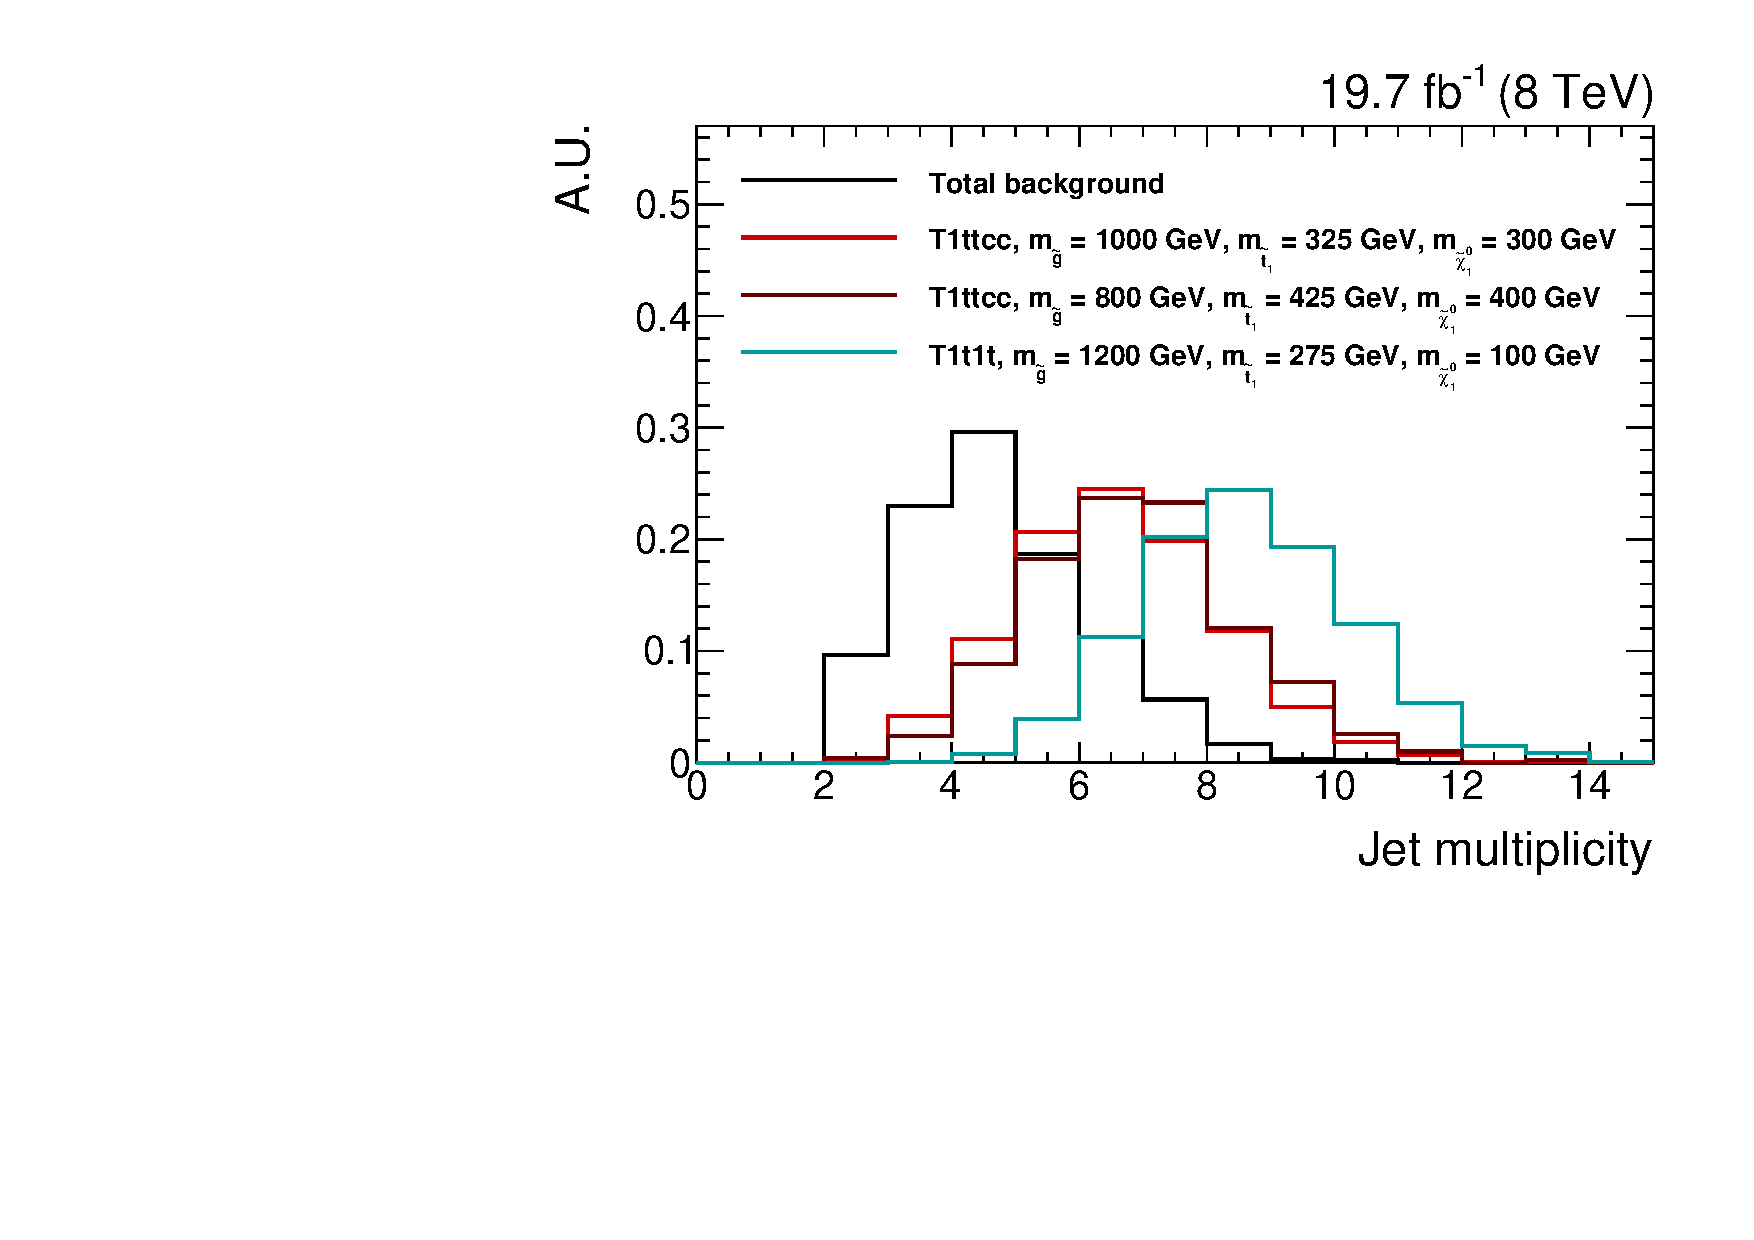
\includegraphics[width=0.6\textwidth]{figures/razor_selection/njets_signal_region}
 \caption{Distribution of the number of jets for the total SM background and three example signal
points in the signal region. The full selection except for the jet multiplicity requirement was
applied. The histograms are normalized to unit area.
 \label{fig:njets_sig_BG}}
\end{figure}

In Fig.~\ref{fig:boost_baseline_dataMC} we compare the observed data to the simulation for
events passing this baseline selection. 
As will be the case for all following comparisons of data versus simulation, the simulation is
scaled to the expected number of events according to the (NN)LO cross section of each process.
In addition, the simulated events are reweighted in order to correct for mismodelling of the
pileup, trigger, $\cPqb$ tagging, top \pt distribution, etcetera. Most of these reweightings are
performed for each region, but for some, such as the $\cPqb$ tagging scale factors, the reweighting
is only applied when the source of the reweighting is used explicitly in the selection. For the
$\cPqb$ tagging this would be a specific requirement or veto on the $\cPqb$-tagged jet
multiplicity. Hence, the reweighting is not applied in the baseline selection region. 
A full overview of these sources of event reweighting is given in
Table~\ref{tab:boost_reweighting}. Each of these sets of event weights has an associated
uncertainty. These will be taken into account as systematic uncertainties on the final background
prediction, as explained in more detail in Section~\ref{sec:boost_systematics}. 
From the figure, we see that there is good agreement between data and simulation for the highest
$\mr$ and $\rsq$ bins, \ie when the contribution of QCD multijet MC is very small. 
For the first $\mr$ and $\rsq$ bins, which are dominated by multijet production, the simulation
underpredicts the data by about 50\%. 

\begin{table}[htpb]
  \caption{Sources of event reweighting, when they are applied, and to which process. 
  \label{tab:boost_reweighting}}
  \begin{center}
  \begin{tabular}{l l l}
    \toprule
    Source & Region & Process \\
    \midrule
    Pileup & All & All \\
    Trigger & All & All \\
    $\cPqb$ tagging & If $\cPqb$ tagging used & All \\
    $\W$ tagging & If $\W$ tagging used & All \\
    Top \pt spectrum & All & $t\bar{t}$ \\
    Initial state radiation & All & Signal \\
    \bottomrule
  \end{tabular}
  \end{center}
\end{table}
 
The data/MC comparison is also displayed in table form. The first section of Table~\ref{tab:cutflow}
shows the expected number of events for the different background processes for several steps in the
baseline cutflow. The entry listed as ``No selection" corresponds to the total number of events
expected when no selection is applied. It is equal to the cross section of the process times the
integrated luminosity. 
The row corresponding to ``$n_{PV} > 0$'' gives the event counts after applying the
cleaning filters, the relevant event reweightings, and the requirement that there be at least one
good primary vertex.
The background composition after the full baseline selection, expressed in percentages, is reported
in Table~\ref{tab:BG_comp_percent}.  

\begin{figure}[htbp]
 \centering
 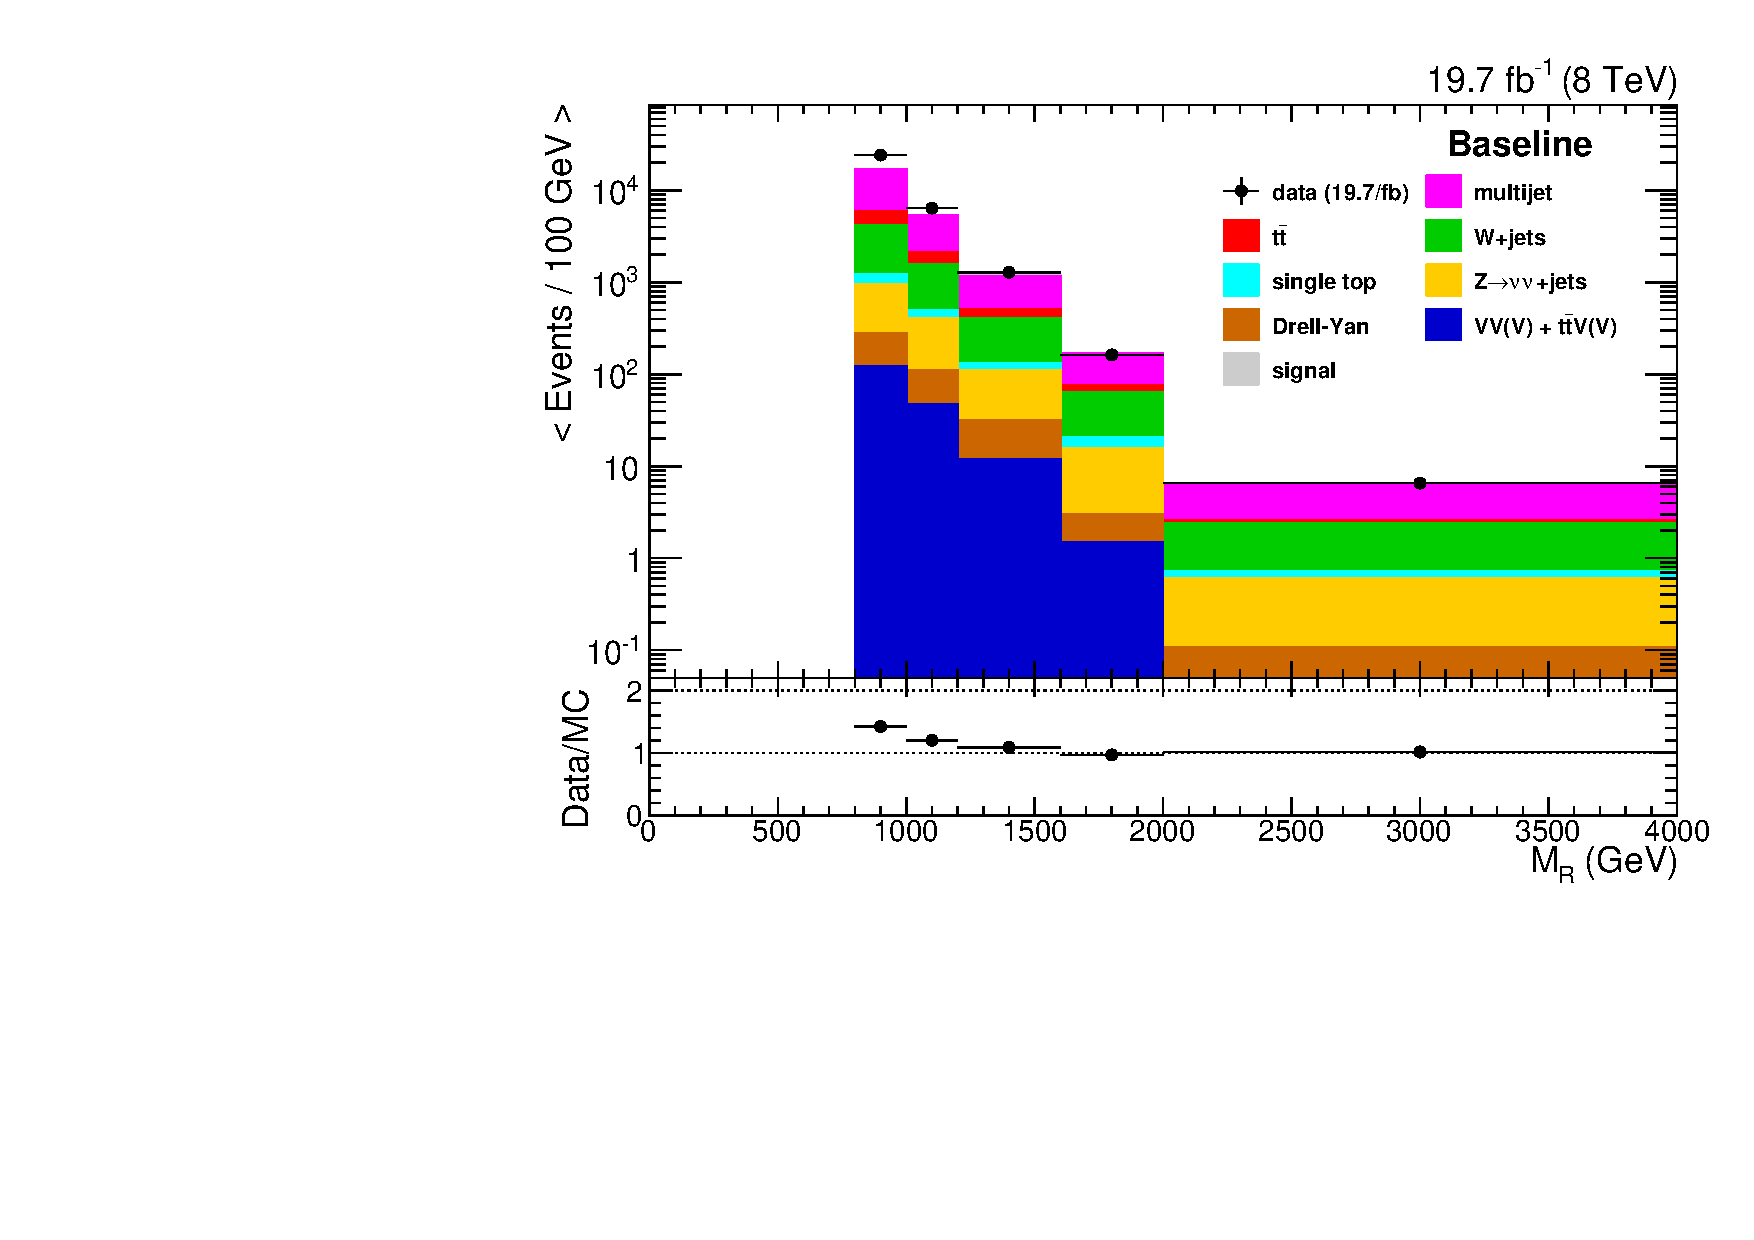
\includegraphics[width=0.48\textwidth]{figures/razor_selection/plots/DataMC_MR_HLT_width}
 ~
 \includegraphics[width=0.48\textwidth]{figures/razor_selection/plots/DataMC_R2_HLT_width}
 \caption{Comparison between data and simulation for the $\mr$ (left) and $\rsq$ (right)
distribution in the baseline selection region. The bin entries are scaled proportional to the bin
width.
 \label{fig:boost_baseline_dataMC}}
\end{figure}


\subsection{Signal region selection \label{sec:boost_signal_selection}}

%%%%%%%%%%%%%%%%%%%%%%
% Signal selection   %
%%%%%%%%%%%%%%%%%%%%%%

The signal region selection aims for a good discrimination between possible signals and the SM
backgrounds. As mentioned before, the signals we target with this search have $\cPqb$ tagged jets
and boosted $\W$ bosons in the final state. Therefore, we require, on top of the baseline
selection, the presence of at least one CSV medium $\cPqb$ tagged jet, and at least one $\W$ boson
tagged jet. AK5 jets are used for $\cPqb$ tagging, whereas for $\W$ tagging we use the CA8 jets, as
explained in Section~\ref{sec:boost_wtag}. 
Additionally, we only consider fully-hadronic events and thus select only those events without
loose electrons or muons, and no isolated tracks. 
These selection criteria already reduce the background substantially, but the achieved signal
separation is not yet sufficient. We need an additional handle on the QCD multijet production,
which is the dominant background at this stage. 

Missing transverse energy, \ETm, in multijet events is largely due to jet mismeasurements,
rather than the escape of weakly interacting particles, such as neutrinos or the neutralinos in
signal events. The \ETm vector will, therefore, often be aligned with one of the jets. 
Based on this we can expect that $\Delta\phi_{min}$, the minimum of the angles between \VEtmiss and
the transverse momentum of the leading three jets, will be a good discriminant between multijet
events and events with real \ETm.
\begin{equation}
 \Delta\phi_{min} = \min_{i=1,2,3}{\Delta\phi(\VEtmiss, \ptvec^{\,i})},
\end{equation}
where $i$ runs over the three leading AK5 jets. We require $\Delta\phi_{min} > 0.5$ to suppress
multijet events. The $\Delta\phi_{min}$ distribution, obtained from simulation, before applying this
selection is shown in
Fig.~\ref{fig:boost_signal_mindeltaphi}. The multijet events are clearly gathered in the first few
bins.

\begin{figure}[htbp]
 \centering
 \includegraphics[width=0.7\textwidth]
 {figures/razor_selection/plots/DataMC_minDeltaPhi_g1Mbg1W0Ll_rebin_nodata}
\caption{Simulated $\Delta\phi_{min}$ distribution with all signal region requirements applied
except $\Delta\phi_{min} > 0.5$. QCD multijet events are clearly gathered in the first few bins.
\label{fig:boost_signal_mindeltaphi}}
\end{figure}

A summary of the signal selection is presented in Table~\ref{tab:boost_selection_summary}.
Figure~\ref{fig:boost_signal_dataMC} shows the simulated distributions in the signal region for the
$\mr$ and $\rsq$ variables. The number of events in simulation and data, and the background
composition in percent, are reported in Table~\ref{tab:cutflow} and
Table~\ref{tab:BG_comp_percent}, respectively. 
The signal region is $t\bar{t}$ dominated, with additional contributions from $\W(\rightarrow
\ell\nu)+$jets and multijet processes.
The \pt distribution of the highest \pt tagged $\W$ boson jet in the event is shown in
Fig.~\ref{fig:boost_signal_Wpt_met}, alongside the \ETm distribution.  

\begin{figure}[htbp]
\centering
\includegraphics[width=0.48\textwidth]
{figures/razor_selection/DataMC_MR_g1Mbg1W0Ll_mdPhig0p5_width_nodata}
~
\includegraphics[width=0.48\textwidth]
{figures/razor_selection/DataMC_R2_g1Mbg1W0Ll_mdPhig0p5_width_nodata}
\caption{Simulated $\mr$ (left) and $\rsq$ (right) distributions in the signal region. An example
signal point, corresponding to the T1ttcc mass point with $m_{\tilde{g}}
\,{=}\, 1\TeV$, $m_{\stopone} \,{=}\, 325\GeV$ and $m_{\lsp} \,{=}\, 300\GeV$, is
stacked on top of the background processes. The bin entries are normalized proportional to the bin
width.  
\label{fig:boost_signal_dataMC}}
\end{figure}

\begin{figure}[htbp]
\centering
\includegraphics[width=0.48\textwidth]
{figures/razor_selection/plots/DataMC_Wpt_g1Mbg1W0Ll_mdPhig0p5_nodata}
~
\includegraphics[width=0.48\textwidth]
{figures/razor_selection/plots/DataMC_met_g1Mbg1W0Ll_mdPhig0p5_nodata}
\caption{Simulated $\W$ tagged jet $\pt$ (left) and $\ETm$ (right) distributions in the signal
region. An example signal point, corresponding to the T1ttcc mass point with $m_{\tilde{g}}
\,{=}\, 1\TeV$, $m_{\stopone} \,{=}\, 325\GeV$ and $m_{\lsp} \,{=}\, 300\GeV$, is
stacked on top of the background processes. 
\label{fig:boost_signal_Wpt_met}}
\end{figure}



% In figures~\ref{fig:DataMC_SignalRegion_MR_R2_mdphig0p5} and \ref{fig:DataMC_SignalRegion_mdphig0p5}
% we show a Data/MC comparison for various quantities for the signal region with $\Delta\phi_{min} >
% 0.5$. 
% Please note that these plots are for illustration purposes only. 
% We will predict the background using data control regions and only use the simulation for
% translation factors between those control regions and the signal region (see further). We stress in
% particular that the QCD multijet MC is underpredicting what we see in data.
% 
% \begin{figure}[p]
%  \includegraphics[width=0.49\textwidth]{figures/DataMC/DataMC_njets_g1Mbg1W0Ll_mdPhig0p5}
%  \includegraphics[width=0.49\textwidth]{figures/DataMC/DataMC_nbjets_g1Mbg1W0Ll_mdPhig0p5}
% 
%  \includegraphics[width=0.49\textwidth]{figures/DataMC/DataMC_met_g1Mbg1W0Ll_mdPhig0p5}
%  \includegraphics[width=0.49\textwidth]{figures/DataMC/DataMC_jet1pt_g1Mbg1W0Ll_mdPhig0p5}
% 
%  \includegraphics[width=0.49\textwidth]{figures/DataMC/DataMC_jet2pt_g1Mbg1W0Ll_mdPhig0p5}
%  \includegraphics[width=0.49\textwidth]{figures/DataMC/DataMC_jet3pt_g1Mbg1W0Ll_mdPhig0p5}
% \caption{For illustration only: Data/MC comparison plot of various event quantities in the signal
% region requiring $\Delta\phi_{min} > 0.5$: 
% [top] jet multiplicity (left) and b-tagged jet multiplicity (right);
% [middle] missing transverse energy (left) and \pt of the highest \pt jet (right);
% [bottom] \pt of the second (left) and third (right) highest \pt jet. 
% \label{fig:DataMC_SignalRegion_mdphig0p5}}
% \end{figure}
% 
% \begin{figure}[htbp]
%  \includegraphics[width=0.49\textwidth]{figures/DataMC/DataMC_Wpt_g1Mbg1W0Ll_mdPhig0p5}
%  \includegraphics[width=0.49\textwidth]{figures/Shapes/comparison_Wpt}
% \caption{For illustration only: [left] Data/MC comparison plot of $\pt(W)$ in the signal region
% requiring $\Delta\phi_{min} > 0.5$.
% [right] Comparison of the $\pt(W)$ distribution for signal and total background. Both distributions
% are normalized to unit area.
% \label{fig:Wpt_SignalRegion}}
% \end{figure}
% 


\subsection{Control region selection \label{sec:boost_control_selection}}

%%%%%%%%%%%%%%%%%%%%%%%%%%%%%%%%%%
% Explanation of control regions
%%%%%%%%%%%%%%%%%%%%%%%%%%%%%%%%%%

The control regions are defined such that they are enriched in one of the three main backgrounds in
the signal region, $t\bar{t}$, QCD multijet, and $\W(\rightarrow \ell \nu)+$jets. The control region
selections will be as close as possible to the signal selection, while maximizing the purity in a
given background process and minimizing possible signal contamination. 
To construct the control regions, different requirements on the 
multiplicity of leptons, $\cPqb$ tagged, and $\W$ tagged jets are placed. 
In the following subsections each control region will be discussed in detail. 

\subsubsection{\texorpdfstring{$T$}{T} region \label{sec:boost_T_region}}

The dominant background in the signal region is $t\bar{t}$ production. We define the $T$ region as a
dedicated control region enriched in this process. 
Similarly to the signal, $t\bar{t}$ events are expected to have $\cPqb$ jets in the final state, as
well as real hadronically decaying $\W$ bosons. We will thus not change those aspects of the signal
selection when defining the $T$ region. 

The main change we do make, is requiring the presence of exactly one loose electron or muon, while
removing the requirement that there be no isolated track. This selection is already sufficient to
obtain a region with a good purity of $t\bar{t}$ events. There is, however, a possibility of
substantial signal contamination. To address this issue, we place an upper boundary on the value of
the transverse mass, $\mT$, computed from the lepton transverse momentum and \VEtmiss, 
\begin{equation}
 \mT = \sqrt{2\pt^\ell\ETm ( 1 - \cos\Delta\phi )},
\end{equation}
with $\Delta\phi$ the difference in azimuthal angle between lepton and \VEtmiss. 
The distribution of $\mT$ exhibits a kinematic edge at the mass of the $\W$ boson for the $t\bar{t}$
process, an edge not present for signal events due to the extra contribution to the \ETm from the
invisible neutralinos.  We require $\mT < 100$\GeV in order to reduce signal contamination and
retain most of the $t\bar{t}$ contribution. The $\mT$ distribution at this selection level is shown
in Fig.~\ref{fig:boost_T_region_mT}. 


\begin{figure}[htbp]
\centering
\includegraphics[width=0.7\textwidth]{figures/razor_selection/DataMC_mT_g1Mbg1W1Ll_rebin}
\caption{Comparison between data and simulation of the $\mT$ distribution in the $T$ region without
any selection on $\mT$ or $\Delta\phi_{min}$. An example signal
point, corresponding to the T1ttcc mass point with $m_{\tilde{g}} \,{=}\, 1\TeV$,
$m_{\stopone} \,{=}\, 325\GeV$ and $m_{\lsp} \,{=}\, 300\GeV$, is stacked on top of
the
background processes. The kinematic edge at the $\W$ boson mass is clearly
visible for the SM backgrounds, whereas the example signal point extends out to high $\mT$.
\label{fig:boost_T_region_mT}}
\end{figure}

The final ingredient for the full $T$ region selection, is the $\Delta\phi_{min} > 0.5$
requirement. This is used to obtain a selection, and thus kinematic properties, as close as
possible to the signal region. The $\Delta\phi_{min}$ distribution is shown in
Fig.~\ref{fig:boost_T_region_mindeltaphi}. A summary of the full $T$ region selection is presented
in Table~\ref{tab:boost_selection_summary}. 


\begin{figure}[htbp]
\centering
\includegraphics[width=0.7\textwidth]
{figures/razor_selection/plots/DataMC_minDeltaPhi_g1Mbg1W1LlmT100_rebin}
\caption{Comparison between data and simulation of the $\Delta\phi_{min}$ distribution in the $T$
region without any selection on $\Delta\phi_{min}$. An example signal
point, corresponding to the T1ttcc mass point with $m_{\tilde{g}} \,{=}\, 1\TeV$,
$m_{\stopone} \,{=}\, 325\GeV$ and $m_{\lsp} \,{=}\, 300\GeV$, is stacked on top of
the
background processes.
\label{fig:boost_T_region_mindeltaphi}}
\end{figure}


Table~\ref{tab:cutflow} shows a breakdown of the contributions of the various background components,
as determined directly from simulation, as wel as the observed data counts, and expected counts for
an example signal point. From Table~\ref{tab:BG_comp_percent} we see that the obtained purity in the
$T$ region is more than 80\% for $t\bar{t}$ and single top processes combined. This is also
illustrated in the $\mr$ and $\rsq$ distributions, as shown on Fig.~\ref{fig:boost_T_region_MR_Rsq}.
There is good agreement between data and simulation in the $T$ region. Any discrepancies can
be accommodated by the systematic uncertainties on the MC, and will not affect the analysis.
We also compare the shape of the $\mr$ and $\rsq$ distributions in the $T$ region versus the $S$
region. We observe from Fig.~\ref{fig:boost_T_region_shape} that the shapes are very similar. This
is important as we will use global transfer factors $\kappa$ to translate between the $T$ and $S$
regions. 


\begin{figure}[htbp]
\centering
\includegraphics[width=0.48\textwidth]
{figures/razor_selection/plots/DataMC_MR_g1Mbg1W1LlmT100_mdPhig0p5_width}
~
\includegraphics[width=0.48\textwidth]
{figures/razor_selection/plots/DataMC_R2_g1Mbg1W1LlmT100_mdPhig0p5_width}
\caption{Comparison between data and simulation of the $\mr$ (left) and $\rsq$ (right)
distribution in the $T$ control region. 
\label{fig:boost_T_region_MR_Rsq}}
\end{figure}

% Comparisons between data and simulation  for various other basic quantities in
% figure~\ref{fig:DataMC_TRegion_mdphig0p5}. 
% 
% \begin{figure}[p]
% \centering
%  \includegraphics[width=0.49\textwidth]{figures/DataMC/DataMC_njets_g1Mbg1W1LlmT100_mdPhig0p5}
%  \includegraphics[width=0.49\textwidth]{figures/DataMC/DataMC_nbjets_g1Mbg1W1LlmT100_mdPhig0p5}
% 
%  \includegraphics[width=0.49\textwidth]{figures/DataMC/DataMC_met_g1Mbg1W1LlmT100_mdPhig0p5}
%  \includegraphics[width=0.49\textwidth]{figures/DataMC/DataMC_jet1pt_g1Mbg1W1LlmT100_mdPhig0p5}
% 
%  \includegraphics[width=0.49\textwidth]{figures/DataMC/DataMC_jet2pt_g1Mbg1W1LlmT100_mdPhig0p5}
%  \includegraphics[width=0.49\textwidth]{figures/DataMC/DataMC_jet3pt_g1Mbg1W1LlmT100_mdPhig0p5}
% \caption{Data/MC comparison plot of various event quantities in the T region: 
% [top] jet multiplicity (left) and b-tagged jet multiplicity (right);
% [middle] missing transverse energy (left) and \pt of the highest \pt jet (right);
% [bottom] \pt of the second (left) and third (right) highest \pt jet. 
% \label{fig:DataMC_TRegion_mdphig0p5}}
% \end{figure}
% 

\begin{figure}[htbp]
\centering
\includegraphics[width=0.48\textwidth]{figures/razor_selection/shapeplots/MR_comparison_TTJ_SIG}
~
\includegraphics[width=0.48\textwidth]{figures/razor_selection/shapeplots/R2_comparison_TTJ_SIG}
\caption{Comparison of the shape of the $\mr$ (left) and $\rsq$ (right) distribution for the
$t\bar{t}$ simulation in the $T$ region versus the $S$ region. The histograms are normalized to
unit area. 
\label{fig:boost_T_region_shape}}
\end{figure}



%%%%%%%%%%%%%%%%%%%%%%%%%%%%%%%%%%%%%%%%%%%%%%%%%%%%%%%%%%%%%%%%%%%%%%%%%%%%%%%%%%%%%%%%%%%%%%%%


\subsubsection{\texorpdfstring{$W$}{W} region}

The second largest background in the signal region comes from $\W(\rightarrow l\nu)$+jets
production, where the lepton from the $\W$ boson decay is lost.
Because the $\W$ boson decays leptonically, any events passing the signal selection necessarily
contain a q/g initiated CA8 jet that is misidentified as a boosted $\W$ boson. 
We do not expect hadronically decaying $\W$ bosons to contribute to the background in the signal
region, as those events would have very small missing energy, in addition to not having real
$\cPqb$ jets. Even though we do not explicitly require a minimal \ETm, our $\rsq$ cut is highly
correlated with \ETm, and induces a minimal cut of around 100\GeV, as can be seen in
figure~\ref{fig:boost_signal_Wpt_met}. 
This expectation was verified by checking the contribution of $\W({\rightarrow}\,
q\bar{q}')b\bar{b}$ using simulation, where it was found that no events pass our signal
selection. 

In order to accurately model the $\W(\rightarrow l\nu)$+jets background, we define a dedicated
control region, the $W$ region, as similar to the signal region as possible. As for the $T$ region,
we require the presence of a loose electron or muon. Additionally we also veto any event that
contains a CSV loose $\cPqb$ tagged jet.  
Since for the $\W(\rightarrow l\nu)$+jets process, there is no real hadronically decaying $\W$
boson, we opt not to use the full $\W$ tagger. 
In order to increase the number of events available in the control region, we require instead the
presence of at least one $\W$ boson mass-tagged jet. This ensures that we are in a kinematically
similar phase space, because we keep the jet mass requirement, but prevents the penalty from
requiring a two-prong decay for a process for which these decays do not occur. 

We also require $\mT < 100$\GeV in order to reduce possible signal contamination. Unlike for the $T$
region, we additionally require $\mT > 30$\GeV in order to reduce remaining contamination from
multijet events. Those events generally have low $\ETm$, which translates in low $\mT$. 
Multijet contamination in the $T$ region is negligible because of the
requirement that there be at least one jet tagged a coming from a $\cPqb$ quark. 
Finally, we also require $\Delta\phi_{min} > 0.5$, as was the case for the signal region. 
A summary of the $W$ region selection is presented in Table~\ref{tab:boost_selection_summary}.

Figure~\ref{fig:boost_W_region_mT} shows the $m_T$ distribution in the $W$ region before making any
selection $\mT$ or on $\Delta\phi_{min}$. The $\Delta\phi_{min}$ distribution in the $W$ region
without applying a selection on $\Delta\phi_{min}$ is given in
Fig.~\ref{fig:boost_W_region_mindeltaphi}. The full breakdown of the backgrounds in this region is
listed in Tables~\ref{tab:cutflow} and \ref{tab:BG_comp_percent}. The $W$ region is about 85\% pure
in the $\W(\rightarrow l\nu)+$jets process. 

\begin{figure}[htbp]
\centering
\includegraphics[width=0.7\textwidth]{figures/razor_selection/plots/DataMC_mT_0Lbg1Y1Ll_rebin}
\caption{Comparison between data and simulation of the $\mT$ distribution in the $W$ region without
any selection on $\mT$ or on $\Delta\phi_{min}$. An example signal
point, corresponding to the T1ttcc mass point with $m_{\tilde{g}} \,{=}\, 1\TeV$,
$m_{\stopone} \,{=}\, 325\GeV$ and $m_{\lsp} \,{=}\, 300\GeV$, is stacked on top of
the background processes.
\label{fig:boost_W_region_mT}}
\end{figure}

\begin{figure}[htbp]
\centering
\includegraphics[width=0.7\textwidth]
{figures/razor_selection/plots/DataMC_minDeltaPhi_0Lbg1Y1LlmT_rebin}
\caption{Comparison between data and simulation of the $\Delta\phi_{min}$ distribution in the $W$
region without any selection on $\Delta\phi_{min}$. 
\label{fig:boost_W_region_mindeltaphi}}
\end{figure}

A comparison between data and simulation for the $\mr$ and $\rsq$ distributions is shown in
Fig.~\ref{fig:boost_W_region_MR_Rsq}. A reasonable agreement is observed. The offset in the
normalization will be absorbed automatically during the background estimation procedure. 
We also compare the shapes of the \mr and \rsq distributions for the $\W(\rightarrow\ell\nu)+$jets
simulation in the $W$ region versus the $S$ region. From Fig.~\ref{fig:boost_W_region_shape} we
observe that there is good agreement, within statistical uncertainties. 
 
\begin{figure}[htbp]
\centering
\includegraphics[width=0.48\textwidth]
{figures/razor_selection/plots/DataMC_MR_0Lbg1Y1LlmT_mdPhig0p5_width}
~
\includegraphics[width=0.48\textwidth]
{figures/razor_selection/plots/DataMC_R2_0Lbg1Y1LlmT_mdPhig0p5_width}
\caption{Comparison between data and simulation of the $\mr$ (left) and $\rsq$ (right)
distributions in the $W$ region. 
\label{fig:boost_W_region_MR_Rsq}}
\end{figure}

% 
% \begin{figure}[p]
% \centering
%  \includegraphics[width=0.49\textwidth]{figures/DataMC/DataMC_njets_0Lbg1Y1LlmT_mdPhig0p5}
% 
%  \includegraphics[width=0.49\textwidth]{figures/DataMC/DataMC_met_0Lbg1Y1LlmT_mdPhig0p5}
%  \includegraphics[width=0.49\textwidth]{figures/DataMC/DataMC_jet1pt_0Lbg1Y1LlmT_mdPhig0p5}
% 
%  \includegraphics[width=0.49\textwidth]{figures/DataMC/DataMC_jet2pt_0Lbg1Y1LlmT_mdPhig0p5}
%  \includegraphics[width=0.49\textwidth]{figures/DataMC/DataMC_jet3pt_0Lbg1Y1LlmT_mdPhig0p5}
% \caption{Data/MC comparison plot of various event quantities in the W region: 
% [top] jet multiplicity;
% [middle] missing transverse energy (left) and \pt of the highest \pt jet (right);
% [bottom] \pt of the second (left) and third (right) highest \pt jet. 
% \label{fig:DataMC_WRegion_mdphig0p5}}
% \end{figure}
% 
\begin{figure}[htbp]
\centering
\includegraphics[width=0.48\textwidth]{figures/razor_selection/shapeplots/MR_comparison_WJ_SIG}
~
\includegraphics[width=0.48\textwidth]{figures/razor_selection/shapeplots/R2_comparison_WJ_SIG}
\caption{Shape of the $\mr$ (left) and $\rsq$ (right) distribution for $\W(\rightarrow
\ell\nu)+$jets simulation in the $W$ region versus the $S$ region. 
\label{fig:boost_W_region_shape}}
\end{figure}

%%%%%%%%%%%%%%%%%%%%%%%%%%%%%%%%%%%%%%%%%%%%%%%%%%%%%%%%%%%%%%%%%%%%%%%%%%%%%%%%%%%%%%%%%%%%%%%%

\subsubsection{\texorpdfstring{$Q$}{Q} region}

The final background for which we define a control region, is QCD multijet production.
To define a region $Q$ enriched in multijet production, we start from the baseline selection, and
add the requirement that there be no loose lepton or isolated track present, as is the case for the
signal region selection. We also veto events containing a CSV loose $\cPqb$ tagged jet. 

Multijet events do not produce $\W$ bosons; any CA8 jet that passes the $\W$ boson tagger,
is thus by definition a misidentified $\W$ boson jet. To reach a similar kinematic phase space as
the signal region, we require that there be at least one $\W$ boson anti-tagged jet. The $\W$ boson
anti-tagging still requires that the jet mass is consistent with the $\W$ boson mass, but inverts
the N-subjettiness requirement. As we do not expect QCD multijet events to have the two-prong
jet-substructure of actual boosted $\W$ bosons, this will enhance the statistical power and purity
of the $Q$ region. 

As explained before, QCD multijet events are expected to have small values for the
$\Delta\phi_{min}$ variable. This can be seen from Fig.~\ref{fig:boost_Q_region_mindeltaphi}. 
For the $Q$ region definition we will thus reverse
and tighten the $\Delta\phi_{min}$ requirement from the signal region. We require $\Delta\phi_{min}
< 0.3$, which results in a very good purity of better than 90\% according to simulation. 
The full breakdown of the backgrounds according to simulation can again be found in
Tables~\ref{tab:cutflow} and \ref{tab:BG_comp_percent}.
Figure~\ref{fig:boost_Q_region_MR_Rsq} shows a comparison between data and simulation for the $\mr$
and $\rsq$ distributions. It is not surprising to observe that the agreement between data and
simulation is not very good. This is a known feature of the QCD multijet simulation, and its
normalisation to LO cross sections. Since we only use ratios of simulated counts in the background
estimation method, and the proportion of multijet events in the signal region is small, the
observed mismodelling will not affect our analysis greatly. 

\begin{figure}[htbp]
\centering
\includegraphics[width=0.7\textwidth]{figures/razor_selection/DataMC_minDeltaPhi_0Lbg1uW0Ll_rebin}
\caption{Comparison between data and simluation of the $\Delta\phi_{min}$ distribution in the $Q$
region before any selection on $\Delta\phi_{min}$. 
\label{fig:boost_Q_region_mindeltaphi}}
\end{figure}

\begin{figure}[htbp]
\centering
\includegraphics[width=0.48\textwidth]
{figures/razor_selection/plots/DataMC_MR_0Lbg1uW0Ll_mdPhi0p3_width}
~
\includegraphics[width=0.48\textwidth]
{figures/razor_selection/plots/DataMC_R2_0Lbg1uW0Ll_mdPhi0p3_width}
\caption{Comparison between data and simulation of the $\mr$ (left) and $\rsq$ (right)
distributions in the $Q$ region. 
\label{fig:boost_Q_region_MR_Rsq}}
\end{figure}

% 
% \begin{figure}[p]
% \centering
%  \includegraphics[width=0.49\textwidth]{figures/DataMC/DataMC_njets_0Lbg1uW0Ll_mdPhi0p3}
% 
%  \includegraphics[width=0.49\textwidth]{figures/DataMC/DataMC_met_0Lbg1uW0Ll_mdPhi0p3}
%  \includegraphics[width=0.49\textwidth]{figures/DataMC/DataMC_jet1pt_0Lbg1uW0Ll_mdPhi0p3}
% 
%  \includegraphics[width=0.49\textwidth]{figures/DataMC/DataMC_jet2pt_0Lbg1uW0Ll_mdPhi0p3}
%  \includegraphics[width=0.49\textwidth]{figures/DataMC/DataMC_jet3pt_0Lbg1uW0Ll_mdPhi0p3}
% \caption{Data/MC comparison plot of various event quantities in the Q region: 
% [top] jet multiplicity;
% [middle] missing transverse energy (left) and \pt of the highest \pt jet (right);
% [bottom] \pt of the second (left) and third (right) highest \pt jet. 
% \label{fig:DataMC_QRegion_mdphi0p3}}
% \end{figure}


In Fig.~\ref{fig:boost_Q_region_shape}, we show a comparison between the shapes of the $\mr$ and
$\rsq$ distributions for the QCD multijet simulation in the signal region versus the $Q$ region.
Given the limited statistical precision for the multijet simulation in the signal region, it is
hard to draw any conclusions from this comparison. Therefore, we also show in
Fig.~\ref{fig:boost_Q_region_shape_no_mindeltaphi} the comparison for the $Q$ and $S$ regions
without selecting a particular $\Delta\phi_{min}$ region. The shape difference in this
region is quite small. As will be explained in Section~\ref{sec:boost_closure_tests}, we will assign
a 40\% systematic uncertainty on the multijet transfer factors in the background prediction to
account for the possible shape difference induced by the $\Delta\phi_{min}$ cut. 

\begin{figure}[htbp]
\centering
\includegraphics[width=0.48\textwidth]{figures/razor_selection/shapeplots/MR_comparison_QCD_SIG}
~
\includegraphics[width=0.48\textwidth]{figures/razor_selection/shapeplots/R2_comparison_QCD_SIG}
\caption{Shape of the $\mr$ (left) and $\rsq$ (right) distribution for the QCD multijet simulation
in the $Q$ region versus the $S$ region. 
\label{fig:boost_Q_region_shape}}
\end{figure}

\begin{figure}[htbp]
\centering
\includegraphics[width=0.48\textwidth]
{figures/razor_selection/shapeplots/MR_comparison_QCD_SIG_no_deltaphimin}
~
\includegraphics[width=0.48\textwidth]
{figures/razor_selection/shapeplots/R2_comparison_QCD_SIG_no_deltaphimin}
\caption{Shape of the $\mr$ (left) and $\rsq$ (right) distribution for the QCD multijet simulation
in the $Q$ region versus the $S$ region with the requirement on  $\Delta\phi_{min}$ removed in both
regions. 
\label{fig:boost_Q_region_shape_no_mindeltaphi}}
\end{figure}

%%%%%%%%%%%%%%%%%%%%%%%%%%%%%%%%%%%%%%%%%%%%%%%%%%%%%%%%%%%%%%%%%%%%%%%%%%%%%%%%%%%%%%%%%%%%%%%%


\begin{table}[thbp]
\centering
\caption{Summary of selection for signal and control regions.
These requirements are in addition to the baseline selection. \label{tab:boost_selection_summary}}
\vspace{1ex}
\begin{tabular}{l cc cc c c}
\toprule
Selection & $S$ & $S'$  & $Q$ & $Q'$ & $T$ & $W$ \\ 
\midrule
nr of $\cPqb$ jets & ${\geq}\, 1$ & ${\geq}\, 1$ & 0 & 0 & ${\geq}\, 1$  & 0 \\
nr of mass-tagged $\W$'s & ${\geq}\,1$ & ${\geq}\,1$ & ${\geq}\,1$ & ${\geq}\,1$ & ${\geq}\,1$ & ${\geq}\,1$ \\
nr of tagged $\W$'s      & ${\geq}\, 1$   & ${\geq}\, 1$   & -   & -     & ${\geq}\, 1$ & - \\
nr of anti-tagged $\W$'s & -          & -          & ${\geq}\, 1$ & ${\geq}\, 1$  & -   & - \\
nr of loose leptons      & 0          & 0          & 0   & 0     & 1             & 1 \\
nr of isolated tracks    & 0          & 0          & 0   & 0     & -             & - \\
$m_T$                    & -          & -          & -   & -     & ${<}\,100$\GeV   & 30--100\GeV\\
$\Delta\phi_{min}$       & ${>}\, 0.5$ & ${<}\, 0.5$ & ${<}\, 0.3$  & ${>}\, 0.5$  & ${>}\, 0.5$ & ${>}\, 0.5$\\
\bottomrule
\end{tabular}
\end{table}

\begin{sidewaystable}[p]
\centering
\caption{Cutflow table, event counts are normalized to $19.7\fbinv$. The signal is the
$m_{\tilde{g}}=1000\GeV$, $m_{\stopone}=325\GeV$, $m_{\lsp}=300\GeV$ point of the
T1ttcc scan. The row corresponding to ``$n_{PV} > 0$'' gives the event counts after applying the
cleaning filters, pileup reweighting, top \pt reweighting for $t\bar{t}$, ISR reweighting for
signal, and the requirement of at least one good primary vertex. The column indicating the total
number of events also includes some smaller processes that only contribute at the early stages of
the event selection. 
The cross sections used for each sample are listed in the second row.}
\vspace{1ex}
{\scriptsize
\begin{tabular}{ l | c  c  c  c  c  c  c  c  c | c  c  c }
%\begin{tabular}{ l || c  c  c  c  c  c  c  c  c | c || c || c }
%\begin{tabular}{| l || c | c | c | c | c | c | c | c | c | c || c || c || c |}
\toprule
Selection & Multijet & $t\bar{t}$ & $\W{\rightarrow}\ell\nu+$jets & Diboson & Single top &
$\cPZ{\rightarrow}\nu\nu+$jets & DY${\rightarrow}\ell\ell+$jets & Triboson & $t\bar{t}V$ & Total &
Signal & Data\\ 
 & $10.4\times 10^7$ pb & 245.8 pb & 111.5 pb & 95.4 pb & 114.9 pb & 588.3 pb & 22.6 pb & 0.69 pb &
1.88 pb & & 0.02435 pb & \\ 
 \midrule
% & 10.4e+07 pb & 245.8 pb & 111.5 pb & 95.4 pb & 114.9 pb & 588.3 pb & 22.6 pb & 0.69 pb & 1.88 pb & 121 pb & & 0.0243547 pb & \\ \hline \hline
No selection & $2.1\times 10^{11}$ & $4.9\times 10^6$ & $2.2\times 10^6$ & $1.9\times 10^6$ & $2.3\times 10^6$ & $1.2\times 10^7$ & $4.5\times 10^5$ & $1.2\times 10^4$ & $3\times 10^4$ & $2.1\times 10^{11}$ & 499 &  \\
$n_{PV} > 0$ & $1.05\times 10^{11}$ & $4.42\times 10^6$ & $2.02\times 10^6$ & $1.08\times 10^6$ & $1.72\times 10^6$ & $2.87\times 10^6$ & $3.7\times 10^5$ & $8.46\times 10^3$ & $2.6\times 10^4$ & $1.05\times 10^{11}$ & 479 & \\
$n_j \geq 3$ & $2.04\times 10^{10}$ & $4.08\times 10^6$ & $1.51\times 10^6$ & $5.19\times 10^5$ & $1.10\times 10^6$ & $6.24\times 10^5$ & $3.06\times 10^5$ & $5.64\times 10^3$ & $2.49\times 10^4$ & $2.05\times 10^{10}$ & 472 &  \\
$\pt(j_1) > 200\GeV$ & $1.82\times 10^8$ & $2.88\times 10^5$ & $4.36\times 10^5$ & $1.86\times 10^4$ & $6.08\times 10^4$ & $5.89\times 10^4$ & $6.61\times 10^4$ & 924 & $5.24\times 10^3$  & $1.82\times 10^8$ & 403 & \\
$M_R \,{>}\, 800, R^2 \,{>}\, 0.08$ & $3.47\times 10^4$ & $5.83\times 10^3$ & $1.17\times 10^4$ & 309 & 900 & $3.25\times 10^3$ & 422 & 40.2 & 183 & 57557 & 224 & \\
Trigger & $3.15\times 10^4$ & $5.12\times 10^3$ & $9.38\times 10^3$ & 249 & 786 & $2.32\times 10^3$ & 367 & 36.4 & 166 & 50164 & 216 & 67037 \\
\midrule
no lepton & $3.09\times 10^4$ & $1.87\times 10^3$ & $3.75\times 10^3$ & 96.3 & 311 & $2.30\times 10^3$ & 145 & 12.6 & 58.5 & 39666 & 142 & 56220 \\
\midrule[.02em]
$n_b \geq 1$ & $9.37\times 10^3$ & $1.51\times 10^3$ & 590 & 25.2 & 226 & 302 & 29.0 & 4.48 & 46.3 & 12187 & 119 & 18164 \\
$n_W \geq 1$ & 841 & 332 & 56.4 & 8.52 & 56.7 & 22.1 & 5.28 & 1.98 & 9.68 & 1350 & 28 & 1817  \\
S & 14.8 & 90.4 & 23.1 & 3.7 & 11.7 & 12.7 & 0.59 & 0.98 & 2.6 & 160 & 23.4 & 187 \\
\midrule[.02em]
$n_b = 0$ & $1.25\times 10^4$ & 98.3 & $1.70\times 10^3$ & 35.6 & 25.9 & $1.25\times 10^3$ & 46.5 & 4.19 & 3.56 & 15691 & 5.65 & 20667 \\
$n_{aW} \geq 1$ & 1519 & 18.7 & 204 & 8.36 & 7.40 & 158 & 5.41 & 0.751 & 0.819 & 1923 & 0.667 & 2712 \\
Q & 1447 & 10.6 & 93.1 & 3.88 & 3.94 & 38.9 & 3.68 & 0.28 & 0.52 & 1603 & 0.07 & 2240 \\
\midrule
1 lepton & 585.9 & $2.74\times 10^3$ & $5.52\times 10^3$ & 132 & 421 & 22.1 & 164 & 19.2 & 88.5 & 9699 & 65.0 & 10008 \\
\midrule[.02em]
$n_b \geq 1$ & 236.7 & $2.17\times 10^3$ & 625 & 29.9 & 301 & 4.14 & 28.7 & 5.36 & 68.3 & 3470 & 54 & 3930 \\
$n_W \geq 1$ & 24.3 & 496 & 61.6 & 10.0 & 50.9 & 0.56 & 3.57 & 2.36 & 16.0 & 666 & 12.3 & 770 \\
T & 0 & 112 & 20.2 & 2.0 & 13.3 & 0 & 0.38 & 0.50 & 3.2 & 151 & 1.2 & 153 \\
\midrule[.02em]
$n_b = 0$ & 150.5 & 153 & $2.86\times 10^3$ & 52.8 & 41.3 & 11.5 & 55.8 & 7.05 & 5.94 & 3329 & 2.54 & 3165 \\
$n_Y \geq 1$ & 30.8 & 79.1 & 605 & 33.1 & 13.8 & 2.4 & 13.1 & 4.57 & 2.61 & 786 & 1.19 & 581 \\
W & 0 & 15.5 & 127 & 3.6 & 1.6 & 0.64 & 0.59 & 0.52 & 0.29 & 150 & 0.06 & 116 \\
\bottomrule
\end{tabular}
}
\label{tab:cutflow}
\end{sidewaystable}

\begin{table}[htpb]
\centering
\caption{Background composition according to simulation
\label{tab:BG_comp_percent}}
\vspace{1ex}
{\small
\begin{tabular}{ l  c  c  c  c  c  c  c }
\toprule
Selection & Multijet & $t\bar{t}$ & $\W(\rightarrow \ell\nu)+$jets & Single top & $\cPZ(\rightarrow
\nu\bar{\nu})+$jets & Diboson & Other \\  
\midrule
Baseline & 62.8\% & 10.2\% & 18.7\% & 1.6\% & 4.6\% & 0.5\% & 1.6\% \\ 
$S$ & 9.2\% & 56.3\% & 14.4\%  & 7.3\% & 7.9\% & 2.3\% & 2.6\% \\
$Q$ & 90.2\% & 0.7\% & 5.8\%  & 0.2\% & 2.4\% & 0.2\% & 0.3\% \\
$T$ & 0.0\% & 73.9\% & 13.3\%  & 8.8\% & 0.0\% & 1.3\% & 2.7\% \\
$W$ & 0.0\% & 10.3\% & 84.8\%  & 1.1\% & 0.4\% & 2.4\% & 1.0\% \\
\bottomrule
\end{tabular}
}
\end{table}




\subsection{Closure tests \label{sec:boost_closure_tests}}

%%%%%%%%%%%%%%%%%%%%%%%%%
% Closure tests
%%%%%%%%%%%%%%%%%%%%%%%%%

In this analysis, we do not explicitly estimate the background in the signal region from the
observations in the control regions. Rather, we create a prior distribution for the four background
components ($t\bar{t}+$single top, $\W(\rightarrow \ell\nu)+$jets, multijet,
and all others) of the signal regions, that incorporates all statistical and systematic
uncertainties, as
will be described in detail in Section~\ref{sec:boost_likelihood}. 
However, in order to verify that the control regions defined in the previous sections provide
adequate data-driven models for the backgrounds in the signal region and that the translations
between different regions behave as expected, we perform two cross checks, taking into account
statistical uncertainties only. 
The first cross check also illustrates the relations between signal and control regions in a more
direct way compared to the full likelihood implementation, where these relations might be less
obvious. 

These cross checks are examples of so-called closure tests. In a closure test, we use our prediction
methods to predict the distributions of some quantity, here the $S$ region backgrounds across the
($\mr, \rsq$) space, in regions similar to the signal region. The predictions are compared with the
observed distributions in these signal-like regions. Discrepancies between the predictions and the
observations are typically the basis of estimates of the systematic uncertainty in the prediction
methods.

\subsubsection{First cross check}

In the first cross check, we predict the background in a signal-like control region, denoted by
$S^\prime$, defined by inverting the $\Delta\phi_{min}$ requirement while preserving the rest of the
selection, see Table~\ref{tab:boost_selection_summary}. 
The estimated number of events, $\widehat{N}$, in the $S^\prime$ region for the QCD multijet,
$\W(\rightarrow \ell\nu)+$jets, and $t\bar{t}$+single top (denoted $t\bar{t}+t$) processes is
computed from the observations, $N_{\rm obs}$, in the $Q$, $T$, and $W$ regions as follows,
\begin{equation}
 \widehat{N}_{\rm QCD}^{S^\prime} = \left( N_{\rm obs}^{Q} - N_{{\rm other, MC}}^{Q} \right)  /
\left(
\frac{N_{\rm QCD}^{Q}}{N_{\rm QCD}^{S^\prime}} \right)_{\rm MC},
\label{eq:E1}
\end{equation}
\begin{equation}
 \widehat{N}_{\W\ell\nu}^{S^\prime} = \left( N_{\rm obs}^{W} - N_{\rm other, MC}^{W} \right) /
\left(
\frac{N_{\W\ell\nu}^{W}}{N_{\W\ell\nu}^{S^\prime}} \right)_{\rm MC},
\label{eq:E2}
\end{equation}
\begin{equation}
  \widehat{N}_{t\bar{t}+t}^{S^\prime} = \left( N_{\rm obs}^{T} - \widehat{N}_{\rm QCD}^{T} - N_{\rm
other, MC}^{T}
\right) / \left( \frac{N_{t\bar{t}+t}^{T}} {N_{t\bar{t}+t}^{S^\prime}}\right)_{\rm MC},
\label{eq:E3}
\end{equation}
where the estimated number of multijet events in the $T$ control region is given by,
\begin{equation}
 \widehat{N}_{\rm QCD}^{T} = \left( N_{\rm obs}^{Q} - N_{\rm other, MC}^{Q} \right) /  \left(
\frac{N_{\rm QCD}^{Q}}{N_{\rm QCD}^{T}} \right)_{\rm MC}.
\label{eq:E4}
\end{equation}
In these equations, $N_{\rm other, MC}$ represents the total contribution of all other processes
apart from the ones mentioned explicitly, as determined from simulation. Because of the purity
of the control regions, these contributions are small. 
As can be seen from Table~\ref{tab:cutflow}, $N_{\rm QCD, MC}^{T} = 0$ for the nominal choice
of systematic uncertainties. The formulae above can thus be simplified since $\widehat{N}_{\rm
QCD}^{T} = 0$. This is, however, not necessarily the case for other choices of systematic
variations.
This relation between the $T$ and $Q$ regions is, therefore, still used to constrain the expected
multijet background in the $T$ region during the final background estimate. 

The total estimated background in the $S^\prime$ region is
\begin{equation}
  \hat{N}^{S^\prime} = \sum_i \hat{N}^{S^\prime}_i , 
\end{equation}
where $i$ runs over all background processes.  For the smaller backgrounds, $\hat{N}^{S^\prime}_i$
is determined by simulation. 
The estimation of backgrounds is done bin-by-bin in the $(\mr,\rsq)$ space. 
However, the estimated transfer factors are global because the statistical precision is not
sufficient to yield reliable bin-by-bin estimates. The expected global transfer factors, which we
will denote by $\kappa$,  are defined in Section~\ref{sec:boost_likelihood}, which also describes
how they are calculated from the simulated data.

Figure~\ref{fig:Shape_syst_1D_project_sideband} shows the projection on the $\mr$ and $\rsq$ axes of
the predicted and observed distributions.  The prediction, which includes only statistical
uncertainties for this cross check, agrees with observation within 20\%. This
test of the background modelling shows that it is feasible to estimate a multicomponent 
background in a signal-like region using the control regions we have defined in
Section~\ref{sec:boost_control_selection}.
In this test, aspects of the modelling in simulation, such as the $\cPqb$ tagging, the translation
between lepton multiplicities, and certain aspects of the $\W$ tagging, have been verified. 

\begin{figure}[tpb]
\includegraphics[width=0.48\textwidth]
{figures/razor_selection/MR_comparison_data_estimate_g1Mbg1W0Ll_mdPhi0p5_log_BPS}
~
\includegraphics[width=0.48\textwidth]
{figures/razor_selection/R2_comparison_data_estimate_g1Mbg1W0Ll_mdPhi0p5_log_BPS}
\caption{Projection of the 2D prediction on the $\mr$ (left) and $\rsq$ (right) axes for the closure
test predicting the $\Delta\phi_{min}$ sideband region $S'$. The uncertainties shown are statistical
only and the horizontal error bars only indicate the bin width.
\label{fig:Shape_syst_1D_project_sideband}}
\end{figure}


\subsubsection{Second cross check}

In a second cross check, we use the $Q$ region to estimate the background in a more signal-like $Q$
region, denoted by $Q^\prime$, where $\Delta\phi_{min} > 0.5$. 
The selection is also summarized in Table~\ref{tab:boost_selection_summary}. 
The estimated background in the $Q'$ region, $\hat{N}^{Q^\prime}$, is computed as
\begin{equation}
  \hat{N}^{Q^\prime} = N_{\rm obs}^Q \frac{N_{\rm MC}^{Q^\prime}}{N_{\rm MC}^Q},
\end{equation}
where $N_{\rm obs}^Q$ is the observed data count in the $Q$ region, and
$N_{\rm MC}$ includes all contributing simulated background processes.

This test assesses the degree to which the simulated distribution of $\Delta\phi_{min}$ as well as
its extrapolation from the $Q$ region, which has $\Delta\phi_{min} < 0.3$, to the $S$ region, with
$\Delta\phi_{min} > 0.5$, are reliable. The comparison between
prediction and observation is shown in Fig.~\ref{fig:Shape_syst_1D_project_QCD}. 
The level of discrepancy, ${\sim}\,40\%$, between the prediction and observation in this cross
check is incorporated as a systematic uncertainty in the global transfer factors. How this is done
technically is described in Section~\ref{sec:boost_likelihood}.

\begin{figure}[htpb]
\includegraphics[width=0.5\textwidth]
{figures/razor_selection/MR_comparison_data_estimate_0Lbg1uW0Ll_mdPhig0p5_from_0Lbg1uW0Ll_mdPhi0p3_log_BPS}
\includegraphics[width=0.5\textwidth]
{figures/razor_selection/R2_comparison_data_estimate_0Lbg1uW0Ll_mdPhig0p5_from_0Lbg1uW0Ll_mdPhi0p3_log_BPS}
\caption{Projection of the 2D prediction on the $\mr$ (left) and $\rsq$ (right) axes for the closure
test predicting the background in region $Q'$, as defined in the text. The uncertainties shown are
statistical only and the horizontal error bars only indicate the bin width.
\label{fig:Shape_syst_1D_project_QCD}}
\end{figure}



\section{Statistical modelling \label{sec:boost_likelihood}}

%%%%%%%%%%%%%%%%%%%%%
% Likelihood stuff
%%%%%%%%%%%%%%%%%%%%%

% TODO \textcolor{red}{This section has been copied directly from the paper draft. It will be
% expanded upon in a next version.}



The statistical analysis of the observations,  $\{ N^S_i \}$, in the signal region is based on a
likelihood function, $L(\sigma)$, given by
\begin{align}
  L(\sigma) & \equiv  \int   \left[ \prod_{i=1}^M p(N^S_i | \sigma, {\cal L}, \theta_i)  \right] 
\pi(\theta) \, \pi({\cal L}) \, d\theta \, d{\cal L},
\label{eq:marginal}
\end{align}
where $\sigma$ is the total signal cross section, $M = 25$ is the number of bins, $N^S_i$ the
observed count in bin $i$, and the bin-by-bin parameters  $\epsilon$,  $b^S_{QCD}, b^S_{TTJ},
b^S_{\W\ell\nu}$, and $b^S_{oth}$ are  denoted collectively by $\theta$. 
The function $\pi({\cal L})$ is the integrated luminosity prior and $\pi(\theta)$ is an evidence
based prior constructed from observations in the control regions and the four global scale factors
$\kappa^{A/B}_{process}$ determined by simulated data. 
The parameter $\epsilon$ represents the $M$ signal efficiencies (including acceptance) for a given
signal model. Figure~\ref{fig:boost_flowchart} shows which control regions provide constraints on
the background parameters, $b^S_{process}$.
The likelihood per bin is taken to be
\begin{equation}
 p(N^S | \sigma, {\cal L}, \theta) = \textrm{Poisson}(N^S,  \epsilon \sigma {\cal L} + b^S_{QCD} +
b^S_{TTJ} + b^S_{\W\ell\nu} +  b^{S}_{oth}) .
\end{equation}

\begin{figure}[p]
  \centering
  \includegraphics[width=\textwidth]{figures/razor_strategy/BoostFlowChart_noZ}
  \caption{Definition of, and relationship between, the signal ($S$) and control ($Q,T,W$) regions
and their relationship to the bin-by-bin background parameters
$b^{\textrm{region}}_{\textrm{process}}$ for a given region and background process, as well as the
four global scale factors $\kappa^{A/B}_{\textrm{process}} = \sum_i b^A_{\textrm{process}, MC, i} /
\sum_i b^B_{\textrm{process}, MC, i}$, where the sum is over all 25 (\mr,\rsq) bins of the simulated
data. 
The total expected background, per bin, is the sum of the terms shown for each region. Furthermore,
associated with each bin of each region is an observed count $N^{\textrm{region}}$, a simulated
count $N^{\textrm{region}}_{\textrm{process}, MC}$, and a count $N^{\textrm{region}}_{oth, MC}$
equal to the sum of the smaller backgrounds, with associated parameter $b^{\textrm{region}}_{oth}$.
  \label{fig:boost_flowchart}}
\end{figure}

The integral in Eq.~(\ref{eq:marginal}) is approximated by Monte Carlo integration by sampling
 the priors $\pi({\cal L})$, and  $\pi(\theta)$. 
The priors for the expected integrated luminosity, ${\cal L}$, signal efficiencies, $\epsilon$, and 
simulated background counts, $b^{region}_{process, MC}$, are modelled with gamma densities,
\begin{align}
\textrm{gamma}(x, \gamma, \beta) &= \beta^{-1}(x/\beta)^{\gamma-1} \exp(-x / \beta) /
\Gamma(\gamma),
\label{eq:gamma}
\end{align}
in which the mode is set to $c$ and the variance to $\delta c^2$, 
where $c \pm \delta c$ denotes either the measured integrated luminosity, or for a given bin of
a given region and process, the simulated signal efficiency, or the simulated background count. This
yields the gamma density parameters,
\begin{align}
   \gamma &= [(k + 2) + \sqrt{(k+2)^2 - 4}]/2,\\
   \beta &= [\sqrt{c^2 + 4\delta c^2} - c]/2,
\end{align}
where $k = (c / \delta c)^2$.
For empty bins, we set $\gamma = 1$ and the bin value is constrained to zero by setting the $\beta$
parameter to $10^{-4}$.
 
For the signal efficiencies and backgrounds, the prior is modelled hierarchically,
\begin{align}
  \pi(\theta) = \int \pi(\theta | c ) \, \pi(c | \phi ) \pi(\phi) \, dc d\phi,
  \label{eq:prior}
\end{align}
where $c$ is a simulated count or efficiency in an $(\mr,  \rsq)$ bin and $\phi$ represents
parameters that characterize the independent sources of systematic uncertainty, described in
Section~\ref{sec:boost_systematics}. 
The integral in Eq.~(\ref{eq:prior}) is evaluated as follows: $\phi$ values are sampled from
$\pi(\phi)$, then $c$ values from $\pi(c | \phi)$, then $\theta$ values from $\pi(\theta | c)$. 
The sampling from $\pi(\phi)$ and $\pi(\theta|c)$ is straightforward because the functional forms
are known. However, the sampling of $c$ requires running the analysis multiple times.
The independent sources of systematic uncertainty are sampled simultaneously, which produces an
ensemble of sets of $(\mr, \rsq)$ histograms for the simulated backgrounds and efficiencies, for all
signals under consideration, that automatically incorporate all statistical dependencies
without the need to model them explicitly.  The ensemble of histograms is the output of the
procedure described in Section~\ref{sec:boost_systematics}. Thereafter, the sampling proceeds as
follows:
\begin{enumerate}
\item sample the integrated luminosity parameter;
\item sample the efficiency parameters, $\epsilon$, for every signal model;
\item sample the parameters $b^{region}_{process, MC}$ of the simulated background densities and sum
their values over the $M$ bins;
\item compute the $\kappa$ parameters from the appropriate background sums (for example,
$\kappa^{Q/S}_{QCD} =  \sum_i  b^Q_{QCD, MC, i} / \sum b^S_{QCD, MC, i}$);
\item scale each $\kappa$ value by a random Gaussian variate of unit mean and standard deviation
of 0.33 to account for additional uncertainty in $\kappa$ due to deficiencies in the simulated
 data, and 
\item sample the background parameters $b^S_{QCD}$, $b^S_{TTJ}$, and $b^S_{\W\ell\nu}$, from the 
Poisson models  of the control regions; for example, for region $Q$, we map  $\textrm{Poisson}(N^Q
, \kappa^{Q / S} b^S_{QCD} + b^Q_{oth})$ to a posterior density in $b^S_{QCD}$ using a flat prior
and sample $b^S_{QCD}$ from that density.
\end{enumerate}

In the absence of  a signal, we determine limits on the total signal cross section using the CLs
criterion~\cite{LHCCLs} and the test statistic $t_\sigma = 2 \ln [ L(\hat{\sigma}) /  L(\sigma)]$
when $0 \leq\hat{\sigma} \leq \sigma$, and $t_\sigma = 0$ when $\hat{\sigma} > \sigma$. 
Large values of $t_\sigma$ indicate incompatibility between the best fit hypothesis $\sigma^\prime 
= \hat{\sigma}$ and the entertained hypothesis $\sigma^\prime  = \sigma$. 
We calculate  the p-values $p_0 = \textrm{Prob}(t_\sigma > t_{\sigma, obs} | \sigma^\prime = 0)$ 
and $p_\sigma = \textrm{Prob}(t_\sigma > t_{\sigma, obs} | \sigma^\prime=\sigma)$, needed to
calculate $\textrm{CLs}(\sigma) = p_\sigma / p_0$,  by simulation. 
The quantity $t_{\sigma, obs}$ denotes the observed values of the test statistic, one for each
hypothesis $\sigma^\prime=\sigma$.




% \section{Likelihood \label{sec:likelihood}}
% 
% \subsection{Introduction \label{sec:intro}}
% The probability model for this analysis consists of a multi-Poisson 
% likelihood for the signal
% region and a prior that models the uncertainties in 
% the integrated luminosity, ${\cal L}$, the signal efficiencies,
% $\epsilon$ (which includes the
% acceptance), and the backgrounds. The total 
% cross section of the signal,
% $\sigma$, is the parameter of interest. The structure of the model is shown in
% Fig.~\ref{fig:BoostWorkflow}. 
% There is one signal region, $S$, in which the search is conducted and three control regions, $Q$,
% $T$, and  $W$, which are used to constrain the expected QCD, top, and W backgrounds,
% $b^S_{QCD}$, $b^S_{TTJ}$, and $b^S_{W\ell\nu}$, respectively,
%  in the signal region~\footnote{In the symbol
%    $X^{region}_{component}$, the superscript labels the region ---
%    either 
% the signal region, $S$,
%  or a control 
% region, $Q$, $T$, or $W$ --- while the subscript labels the background
% component 
% within the region. Since this analysis uses both real
%  and simulated data, we distinguish symbols pertaining to simulated
%  data  by 
% appending the subscript $MC$.}.
% Simulated data in each of the four
% regions are used to constrain the
% small expected 
% background counts $b_{oth}^j$, $j = S, Q, T, W$ and
% four global scale factors 
% $\kappa^{Q/S}_{QCD}$,  $\kappa^{T/S}_{TTJ}$, $\kappa^{Q/T}_{QCD}$, and
% $\kappa^{W/S}_{QW\ell\nu}$, defined as the ratio of the expected background
% component in a control region to that in the signal (or another control) region.
% For example, the factor $\kappa^{Q/S}_{QCD}$ is the ratio of the
% expected 
% QCD background
% in the $Q$ region to that in the $S$ region. The scale factors can
% be estimated by the inverse of the MC ratios defined in
% Eqs.~(\ref{eq:E1})--(\ref{eq:E4})~\footnote{These
% ratios, which are ratios of
% MC counts, 
% $N^{region}_{component, MC}$ are not used in the model; rather 
% the model is written in terms of the $\kappa$ parameters.}. As noted
% above, global scale factors are used because 
% the statistical precision of some of the
% simulated data precludes the use bin-by-bin scale
% factors. Deficiencies in MC modeling are accounted for by assigning 
% appropriate uncertainties to the global factors, as described in 
% Section~\ref{sec:systematics}.
% 
% 
% 
% Below, we give
% brief 
% descriptions of each of the four 
% regions and provide some details of the statistical modeling. 
% In subscripts, the top contribution is
% written
% as $TTJ$, rather than $TTJ+T$, where it is to be understood that the
% top
% contribution includes single top.
% 
% \subsection{Signal Region}
% 
% Tthe background in the signal region is divided into four components,
% \begin{enumerate}
% 	\item QCD
% 	\item TTJets + T
% 	\item WJets
% 	\item Other (VV, VVV, TTX, Zll, Wbb, Z$\nu\nu$),
% \end{enumerate}
% with expected (i.e., mean) count per bin $b^S_{QCD}$, $b^S_{TTJ}$, $b^S_{Wl\nu}$, and
%  $b^S_{oth}$, respectively. 
% The quantities pertaining to the signal region are:
% \begin{align}
%  \textrm{\bf components}\nonumber\\
%  \textrm{QCD, TTJets+T, WJets, Other}\nonumber\\
%  %
%   \textrm{\bf observed count} 	& \quad\textrm{\bf expected count} \nonumber\\
%   	N^S 
% 	&\quad \sigma \epsilon {\cal L} + b^S_{QCD} + b^S_{TTJ} +
%         b^S_{Wl\nu} +  b^{S}_{oth, MC} 
% 	\nonumber\\
% %
% 	\textrm{\bf MC counts}	& \quad\textrm{\bf expected counts}	
% 	\nonumber\\
% 	N^{S}_{QCD, MC} 		& \quad b^{S}_{QCD, MC}
% 		\nonumber\\ 
% 	N^{S}_{TTJ, MC} 		& \quad b^{S}_{TTJ, MC}  
% 			\nonumber\\ 
% 	N^{S}_{W\ell\nu, MC} 	& \quad b^{S}_{W\ell\nu, MC} 
% 		\nonumber\\ 		
% 	N^{S}_{oth, MC} 		& \quad b^{S}_{oth, MC}	
% \end{align}
% The likelihood per bin is given by, 
% \begin{align}
%   p(N^S| \sigma, \theta) = \textrm{Poisson}(N^S,  \sigma \epsilon {\cal L} + b^S_{QCD} + b^S_{TTJ}
%+ b^S_{Wl\nu} +  b^{S}_{oth, MC}),
%   \label{eq:likelihood}
% \end{align}
% where $\theta$ denotes the nuisance
% parameters $\epsilon$, ${\cal L}$, $b^S_{QCD}, b^S_{TTJ}$,
% $b^S_{Wl\nu}$, and $b^S_{oth, MC}$. 
% The integrated
%  luminosity, the signal efficiency, and the
% simulated background, are modeled 
% with gamma densities, Eq.~(\ref{eq:gamma}).
% 
% 
% \subsection{Control Regions}
% The data counts in a control region are modeled with Poisson distributions, 
% while the
% simulated backgrounds are modeled 
% with gamma densities, Eq.~(\ref{eq:gamma}).
%  
% \paragraph*{Q Region}
% For each bin, this region constrains the parameter $b^S_{QCD}$, given
% $N^Q$, $b^Q_{oth, MC}$ and $\kappa^{Q/S}_{QCD}$.
%  \begin{align}
%  \textrm{\bf components}\nonumber\\
%  \textrm{QCD, Other}\nonumber\\
%  %
%   \textrm{\bf observed count} 	& \quad\textrm{\bf expected count}
%   \nonumber\\
%  	N^Q 					& \quad\kappa^{Q/S}_{QCD} \, b^S_{QCD}  + 
%b^{Q}_{oth, MC} 
% 	\nonumber\\ 
% %
% 	\textrm{\bf MC counts}	& \quad\textrm{\bf expected counts}
% 	\nonumber\\
% 	N^{Q}_{QCD, MC} 		& \quad b^Q_{QCD,MC} = \kappa^{Q/S}_{QCD} \, b^{S}_{QCD, MC}
% 	\nonumber\\ 	
% 	N^{Q}_{oth, MC} 		&\quad b^{Q}_{oth, MC}	
% \end{align}
% 
% \paragraph*{T Region}
% For each bin, this region constrains the parameter $b^S_{TTJ}$, given
% $N^T$, $b^T_{oth, MC}$, $b^S_{QCD}$,  $\kappa^{T/S}_{TTJ}$,
% $\kappa^{T/Q}_{QCD}$, 
% and $\kappa^{Q/S}_{QCD}$.
%  \begin{align}
%  \textrm{\bf components}\nonumber\\
%  \textrm{TTJets, QCD, Other}\nonumber\\
%  %
%   \textrm{\bf observed count} 	& \quad\textrm{\bf expected count}
%   \nonumber\\
%  	N^T 					& \quad\kappa^{T/S}_{TTJ} \, b^S_{TTJ}  
% 	+ \kappa^{T/Q}_{QCD} \, \kappa^{Q/S}_{QCD} \, b^S_{QCD}  
% 	+  b^{T}_{oth, MC} 
% 	\nonumber\\ 
% %
% 	\textrm{\bf MC counts}	& \quad\textrm{\bf expected counts}
% 	\nonumber\\
% 	N^{T}_{TTJ, MC} 		& \quad b^T_{TTJ, MC} = \kappa^{T/S}_{TTJ} \, b^{S}_{TTJ,
%MC}
% 	\nonumber\\ 
% 	N^{T}_{QCD, MC} 		& \quad b^T_{QCD, MC} = \kappa^{T/Q}_{QCD} \,
%\kappa^{Q/S}_{QCD} \, b^{S}_{QCD,MC}  
% 	\nonumber\\ 	
% 	N^{T}_{oth, MC} 		&\quad b^{T}_{oth, MC}
% \end{align}
% 
% \paragraph*{W Region}
% For each bin, this region constrains the parameter $b^S_{W\ell\nu}$, given
% $N^W$, $b^W_{oth, MC}$ and $\kappa^{W/S}_{W\ell\nu}$.
%  \begin{align}
%  \textrm{\bf components}\nonumber\\
%  \textrm{WJets, Other}\nonumber\\
%  %
%   \textrm{\bf observed count} 	& \quad\textrm{\bf expected count}
%   \nonumber\\
%  	N^W					& \quad\kappa^{W/S}_{W\ell\nu} \, b^S_{W\ell\nu}    
% 	+  b^{W}_{oth, MC} 
% 	 \nonumber\\ 
% %
% 	\textrm{\bf MC counts}	& \quad\textrm{\bf expected counts}\nonumber\\
% 	N^{W}_{W\ell\nu, MC} 	& \quad b^W_{W\ell\nu, MC} = \kappa^{W/S}_{W\ell\nu} \,
%b^{S}_{W\ell\nu, MC}
% 	 \nonumber\\ 
% 	N^{W}_{oth, MC} 		&\quad b^{W}_{oth, MC}
% \end{align}
% 
% \subsection{Priors
% \label{sec:priors}}
% The integrated luminosity, the signal efficiencies, and 
% the simulated background counts --- where $c \pm \delta c$ denotes the
% value in an $(\mathrm{M_R}, \mathrm{R^2})$ bin
% and its
% uncertainty --- are modeled with gamma priors of the form, 
% \begin{align}
% \beta^{-1}(x/\beta)^{\gamma-1} \exp(-x / \beta) / \Gamma(\gamma),
% \label{eq:gamma}
% \end{align}
% in which the mode is set to $c$
% and the variance to $\delta c^2$, yielding 
%  \begin{align}
%  	\gamma &= [(k + 2) + \sqrt{(k+2)^2 - 4}]/2,\\
% 	\beta &= [\sqrt{c^2 + 4\delta c^2} - c]/2,
%  \end{align}
% for the gamma density parameters,
%  where $k = (c / \delta c)^2$. For empty bins, $\gamma = 1$ and the bin value is
%  constrained to zero by 
%  setting the $\beta$ parameter to $10^{-4}$.
%  
% \subsection{Final likelihood}
% Several systematic uncertainties in this analysis induce
% correlations
% across the bins of all signal and background models. A canonical example
% is the jet energy scale, which when varied 
% induces coherent shifts in the signal and background
% models. The standard way to
% handle these shifts is to model explicitly (by fitting a large number
% of empirical functions) the
% dependence of the likelihood parameters on the parameters of the underlying sources of
% uncertainty and by making assumptions about how parameters
% are correlated. 
% 
% In this analysis, we  approach the problem
% differently. 
% Uncertainties are accounted for by 
% marginalizing,
% \begin{align}
%   p(D^S| \sigma)	 & = \int   \left[\prod_{i=1}^M p(N^S_i|
%     \sigma, \theta)\right] 
% \pi(\theta) \, d\theta,
% \label{eq:marginal}
% \end{align}
%  the likelihood $p(D^S|\sigma, \theta)$ 
% with respect to an evidence based
% prior $\pi(\theta)$, where $D^S \equiv N^S_1,\cdots, N^S_K$ and $K = 25$
% is
% the number of bins. 
% The integral
% is approximated by Monte Carlo integration,
% \begin{align}
%     p(D^S| \sigma) & \approx \frac{1}{J} \sum_{j=1}^J \prod_{i=1}^K
%     p(N^S_i| \sigma, \theta_j),
% \end{align}
% using $J$ points $\theta_j$ randomly sampled from the prior
% $\pi(\theta)$. Since the
% background model closely matches the data, the points
% $\theta_j$ are well matched to the likelihood. Consequently, 
% with a few hundred 
% points,
% Monte Carlo integration
% provides a good approximation to the integral in Eq.~(\ref{eq:marginal})
% 
% In practice, the prior $\pi(\theta)$ is modeled
% hierarchically,
% \begin{align}
%   \pi(\theta) = \int \pi(\theta | c ) \, \pi(c |
%   \phi ) \pi(\phi) \, dc d\phi,
%   \label{eq:prior}
% \end{align}
% where, again, $c$ is an $(\mathrm{M_R},  \mathrm{R^2})$ bin value 
% and $\phi$ represents parameters that characterize the independent
% sources
% of systematic uncertainty. The integral in Eq.~(\ref{eq:prior}) is
% evaluated
% as follows: one samples $\phi$
% values from
% $\pi(\phi)$,
% then $c$ values from $\pi(c | \phi)$, then $\theta$ values from
% $\pi(\theta | c)$. The sampling from $\pi(\phi)$ and $\pi(\theta|c)$
% is straightforward because the functional forms are known. However, 
% the sampling of $c$ requires running the analysis multiple times.
% 
% 
% One crucial difference with respect to the standard method
% is that we 
% sample \emph{simultaneously} from the priors of the
% independent sources of uncertainty (see
% Section~\ref{sec:systematics}). 
% This procedure produces an
% ensemble of sets of $(\mathrm{M_R}, \mathrm{R^2})$ histograms for
% the simulated backgrounds and the efficiencies for all signals
% under
% consideration. Thereafter, the sampling proceeds as follows. 
% For a given set of $c \pm \delta c$ values:
% \begin{enumerate}
% \item sample the integrated luminosity parameter;
% \item sample the efficiency parameters for every signal model;
% \item sample the parameters $b^{region}_{component, MC}$ of the
% background densities and sum their values over bins;
% \item compute the $\kappa$ parameters from the appropriate 
% background sums (for example,
% $\kappa^{Q/S}_{QCD}$  is given by the ratio $\sum  b^Q_{QCD, MC} /
% \sum b^S_{QCD,
%   MC}$), and 
% \item sample the 
% background parameters of the signal region, $b^S_{QCD}$, $b^S_{TTJ}$,
% and
% $b^S_{W\ell\nu}$, 
% from the 
% Poisson
% models of the control regions~\footnote{The Poisson is
%   inverted
% using Bayes theorem and a flat prior and the background parameter
% is sampled.}. 
% \end{enumerate}
% This sampling technique automatically accounts for all correlations, across 
% all bins, all backgrounds, and all signal models and automatically
% includes any non-Gaussian effects.
% 


% appendix on likelihoods and CLs?


\section{Systematic uncertainties \label{sec:boost_systematics}}

% add details on different sources
% add info on various extra studies

% %%%%%%%%%%%%%%%%%%%%%%%%%%%
% % Systematic uncertainties
% %%%%%%%%%%%%%%%%%%%%%%%%%%%

 
The input to the statistical analysis is an ensemble of histograms in the $(\mr,\rsq)$ plane that 
incorporates systematic uncertainties in the simulated signal and background samples.  
The independent systematic effects, described below, are sampled simultaneously. 
This is one of the characteristics that sets this analysis apart. 
For each sampled systematic effect, the same zero mean, unit variance, Gaussian variate is used in
the calculation of the random shift of the systematic effect for all the signal and background
models. Likewise, the same randomly sampled parton distribution functions are used for each event
and for all signal and background models. 
In this way, the statistical dependencies among all bins of the signal and background models are
correctly, and automatically, modelled. The sampling of the systematic effects
is repeated several hundred ($J$) times.  
In all cases, except for the PDFs, the systematic uncertainties are in the scale factors 
applied to the simulated samples to correct them for modelling deficiencies. 
In the next subsections I will discuss each source of systematic uncertainty in more detail. 


%%%%%%%%%%%%%%%%%%%%%%%%%%%%%%%%%%%%%%%%%%%%%%%%%%%%%%%%%%%%%%%%%%%%%%%%%%%%%%%%%%%%%%%%%%%%%%%%%%%%
\subsection{Jet energy scale corrections \label{sec:boost_JEC}}  

Jet energy scale corrections (JEC) map the measured jet energy deposition in the detector back to
the particle level. Within CMS the JEC are applied in sequential levels, each correcting for a
different effect. Details on the various levels were given in Section~\ref{sec:object_jets}.
For our discussion here, the important thing to remember is that each level of correction is simply
a scaling of the four-momentum of the jet by a scale factor that depends on the jet \pt and $\eta$.

Uncertainties in JEC originate from various uncorrelated sources.   
Given $M$ such sources, the full correction on the \pt of a jet, according to a random shift
within the uncertainties, becomes 
\begin{equation}
s(\pt, \eta, \alpha_i) = \sum_{i=1}^M \alpha_i S_i (\pt, \eta)
\end{equation}
where $S_i (\pt, \eta)$ is a \pt and $\eta$-dependent JEC uncertainty for a source $i$ and
$\alpha_i$ are weights randomly sampled from a Gaussian distribution with zero mean and unit
width. 
Here, the weights $\alpha_i$ are different for each source, but are universal for each jet and each
event when considering a given systematic sampling.
Dealing with the myriad of uncertainty sources is not so straightforward in practice, and also not
necessary for a new physics search. As recommended by the POG providing the jet energy scale
corrections and uncertainties, we will therefore take a much simpler approach, using a total
uncertainty $S (\pt, \eta)$ and a random number $\alpha$ from a single Gaussian,
\begin{equation}
s(\pt, \eta, \alpha) = \alpha S (\pt, \eta) = \alpha \sqrt {\sum_i^M s_i^2 (\pt, \eta) }.
\end{equation}
The jet $p_T$ for a given random variation becomes:
\begin{equation}
\pt^{\rm corr} = \left(1 + s(\pt, \eta, \alpha)\right) \pt^{\rm orig}.
\end{equation}
This calculation is repeated $J$ times, each time using a different number sampled from the
Gaussian.  
The overall effect of the JEC uncertainty on a given yield is obtained from the distribution of
the resulting $J$ yields.  
As was done for the jet energy scale corrections themselves, the associated uncertainties are also
propagated to the \VEtmiss.


%%%%%%%%%%%%%%%%%%%%%%%%%%%%%%%%%%%%%%%%%%%%%%%%%%%%%%%%%%%%%%%%%%%%%%%%%%%%%%%%%%%%%%%%%%%%%%%%%%%%
\subsection{Parton distribution functions \label{sec:boost_pdf_unc}} 

In order to evaluate the systematic uncertainty arising from imperfect knowledge of the parton
distribution functions, we use three PDF sets, {\tt CT10}~\cite{Lai:2010vv}, {\tt
MSTW2008lo68cl}~\cite{Martin:2009iq},
 and {\tt NNPDF23\_lo\_as\_0130\_qed}~\cite{nnpdf}, which are
recommended by the PDF4LHC group~\cite{Alekhin:2011sk,Botje:2011sn}.  
Since we take into account full correlations within systematic variations, we need a way to sample
randomly also from the PDF uncertainties, such that the PDF variations can be incorporated directly
in our workflow. 
Of the three recommended PDF sets, {\tt NNPDF} already presents the PDF eigenvectors as a randomly
distributed set, while the other groups provide eigenvectors obtained by varying the PDF fit
parameters by $\pm 1$ standard deviation.  
However, the recently developed {\tt LHAPDF6}~\cite{LHAPDF6} offers a formal way to convert the
latter sets into the randomly distributed sets we need.  
We have used the program {\tt hessian2replicas} to generate randomly
distributed PDF sets with 100 members each, for both {\tt CT10} and {\tt MSTW2008lo68cl}.  

Given a sampled set $i$, for PDF set $K$, and the PDF set $O$ with which the events were simulated,
events are reweighted using the scale factors, 
\begin{equation}
{\rm SF}_{K, i} = \frac{w_{K, i}}{w_{O}},
\end{equation}
where the weights $w$ are products of the event-by-event PDFs for both colliding partons.
The PDF set $O$ was listed for each sample in Section~\ref{sec:boost_mc_samples}.
The overall PDF uncertainty in the background counts or signal efficiencies is derived
from the distribution of ${\rm SF}_{K, i}$ obtained by a random selection of $K$ and $i$.  

To study the effect of the different PDF sets on the simulated counts used in the background
estimation, we compute the distribution of simulated counts corresponding to a random selection of
PDF members from the three PDF sets. 
A Gaussian distribution is then fitted to these distributions. Its width indicates the uncertainty
induced by the given PDF set. 
Figures~\ref{fig:PDF_effect_on_bg_QCD}-\ref{fig:PDF_effect_on_bg_oth2} show the result of this
procedure for the simulated background counts that are used to compute the transfer factors
$\kappa$. 
There is a Gaussian distribution for each PDF set, and the arrow indicates the value for a given
count as obtained using the PDF set that was used during the generation of the MC samples. 
From these figures we conclude that the overall systematic uncertainty resulting from the parton
distribution functions on the background counts is due to both the difference in the nominal values
of the PDF sets, and the spread within the separate PDF sets.

Figure~\ref{fig:PDF_effect_on_sig} shows the equivalent for an example signal point. Here we see
that the spread of the {\tt CT10} PDF dominates the total uncertainty in the signal efficiency. 
We also note that we have computed the signal efficiencies with respect to the nominal PDF set
member of the given PDF rather than the original PDF used for the generation of the samples.
This is done to make sure that only the PDF effects on the acceptance are included in the
experimental uncertainties. The PDF effect on the expected signal cross section is taken into
account separately.

\begin{figure}[p]
\centering
\includegraphics[width=0.48\textwidth,clip=true,trim=0 0.2cm 0 1.2cm]
{figures/razor_systematics/h_S_QCD_MC}
~
\includegraphics[width=0.48\textwidth,clip=true,trim=0 0.2cm 0 1.2cm]
{figures/razor_systematics/h_Q_QCD_MC}
\caption{Influence of different PDF sets on the MC counts entering $\kappa_{\rm QCD}^{Q/S}$.
\label{fig:PDF_effect_on_bg_QCD}}
%\end{figure}
\vspace{2eM}
%\begin{figure}[htpb]
%\centering
\includegraphics[width=0.48\textwidth,clip=true,trim=0 0.2cm 0 1.2cm]
{figures/razor_systematics/h_S_TTJ_MC}
~
\includegraphics[width=0.48\textwidth,clip=true,trim=0 0.2cm 0 1.2cm]
{figures/razor_systematics/h_T_TTJ_MC}
\caption{Influence of different PDF sets on the MC counts entering $\kappa_{t\bar{t}+t}^{T/S}$.
\label{fig:PDF_effect_on_bg_TTJ}}
%\end{figure}
\vspace{2eM}
%\begin{figure}[htpb]
%\centering
\includegraphics[width=0.48\textwidth,clip=true,trim=0 0.2cm 0 1.2cm]
{figures/razor_systematics/h_S_Wlv_MC}
~
\includegraphics[width=0.48\textwidth,clip=true,trim=0 0.2cm 0 1.2cm]
{figures/razor_systematics/h_W_Wlv_MC}
\caption{Influence of different PDF sets on the MC counts entering $\kappa_{\W\ell\nu}^{W/S}$.
\label{fig:PDF_effect_on_bg_Wlv}}
\end{figure}


\begin{figure}[p]
\centering
\includegraphics[width=0.48\textwidth,clip=true,trim=0 0.2cm 0 1.2cm]
{figures/razor_systematics/h_S_oth_MC}
~
\includegraphics[width=0.48\textwidth,clip=true,trim=0 0.2cm 0 1.2cm]
{figures/razor_systematics/h_T_oth_MC}
\caption{Influence of different PDF sets on the MC counts in the $S$ (left) and $T$ (right) region
for the backgrounds that are taken directly from the simulation.
\label{fig:PDF_effect_on_bg_oth1}}
%\end{figure}
\vspace{2eM}
%\begin{figure}
%\centering
\includegraphics[width=0.48\textwidth,clip=true,trim=0 0.2cm 0 1.2cm]
{figures/razor_systematics/h_W_oth_MC}
~
\includegraphics[width=0.48\textwidth,clip=true,trim=0 0.2cm 0 1.2cm]
{figures/razor_systematics/h_Q_oth_MC}
\caption{Influence of different PDF sets on the MC counts in the $W$ (left) and $Q$ (right) region
for the backgrounds that are taken directly from the simulation.
\label{fig:PDF_effect_on_bg_oth2}}
%\end{figure}
\vspace{2eM}
%\begin{figure}
%\centering
\includegraphics[width=0.48\textwidth,clip=true,trim=0 0.2cm 0 1.2cm]
{figures/razor_systematics/h_S_T1ttcc_DM25_1000_300}
\caption{Influence of different PDF sets on the signal efficiency for the T1ttcc signal point with
$m_{\tilde{g}}=1000\GeV, m_{\tilde{t}_1}=325\GeV, m_{\tilde{\chi}_1^0}=300\GeV$. 
\label{fig:PDF_effect_on_sig}}
\end{figure}


%%%%%%%%%%%%%%%%%%%%%%%%%%%%%%%%%%%%%%%%%%%%%%%%%%%%%%%%%%%%%%%%%%%%%%%%%%%%%%%%%%%%%%%%%%%%%%%%%%%%
\subsection{Trigger efficiency}  

Simulated events are weighted by a trigger efficiency, $\epsilon_{\rm trig}$, according to their
values of $\HT$ and first jet \pt (see Section~\ref{sec:boost_data_trigger}). These trigger weights
have an associated uncertainty coming from the statistical precision of the data samples used to
perform the measurement, and the effect of changing the analysis level selection used to measure the
efficiency. The trigger efficiency uncertainty in each bin, as a function of $\HT$
and leading jet $\pt$, is taken to be the maximum of the statistical uncertainty in the efficiency
after imposing the baseline selection and the difference between the efficiencies before and after
applying the baseline selection. 
Magnitudes of the plus and minus uncertainties, $\delta\epsilon^+_{\rm trig}$ and
$\delta\epsilon^-_{\rm trig}$, were shown in Fig.~\ref{fig:boost_trigger_efficiency_unc}.
The event weight $w_{\rm trig}$ to be applied to the simulated events corresponding to a given
systematic sampling is computed based on the efficiency and uncertainty as follows:
\begin{eqnarray}
w_{\rm trig} & = & \epsilon_{\rm trig}(\HT, \pt^{{\rm j}_1}) + \sigma_{\rm trig}
\delta\epsilon^+_{\rm trig}(\HT, \pt^{{\rm j}_1}), \,\,\, {\rm if} \,\, \sigma_{\rm trig} > 0 \\ 
w_{\rm trig} & = & \epsilon_{\rm trig}(\HT, \pt^{{\rm j}_1}) + \sigma_{\rm trig}
\delta\epsilon^-_{\rm trig}(\HT, \pt^{{\rm j}_1}), \,\,\, {\rm if} \,\, \sigma_{\rm trig} < 0 
\end{eqnarray}
where $\sigma_{\rm trig}$ is the random Gaussian number associated to that particular
systematic sampling.	


%%%%%%%%%%%%%%%%%%%%%%%%%%%%%%%%%%%%%%%%%%%%%%%%%%%%%%%%%%%%%%%%%%%%%%%%%%%%%%%%%%%%%%%%%%%%%%%%%%%%
\subsection{\texorpdfstring{$\cPqb$}{b} tagging \label{sec:boost_btag_sf}} 

The $\cPqb$ tagging performance differs between data and simulation, and differs further between 
CMS FullSim and FastSim.  
The simulated events are therefore corrected by applying data/FullSim and FullSim/FastSim $\cPqb$
tag efficiency scale factors, which depend on the flavour, \pt, and $\eta$ of the jets in the
event. 

There are several methods available to reweight events using the $\cPqb$ tag SFs provided by the CMS
BTAG group~\cite{BTagSF1}. 
Here we choose a method where we consider the number of $\cPqb$ tagged jets in an event to be fixed
to what is given by simulation.  
For a given event, the $\cPqb$-tagging efficiencies for truth $\cPqb$, $\mathrm{c}$ and
$\mathrm{udsg}$ jets, corresponding to the relevant tagging algorithm and working point, are used to
compute the probability that the event has the given $\cPqb$ tagged jet multiplicity. 
We compute $P({\rm sim})$ using efficiencies, $\epsilon^{\rm sim}$, obtained from simulated events,
and we obtain $P(\rm data)$ using efficiencies, $\epsilon^{\rm data}$, that represent data,
\begin{eqnarray}
P(\rm sim) & = & \prod_{i} \epsilon_i^{\rm sim} \prod_{j} (1 - \epsilon_j^{\rm sim}) \\
P(\rm data) & = & \prod_{i} \epsilon_i^{\rm data} \prod_{j} (1 - \epsilon_j^{\rm data})
\end{eqnarray}
where
\begin{equation}
\epsilon^{\rm data} = {\rm SF}^{\rm data}_{\rm sim} \epsilon^{\rm sim} ,
\end{equation}
$i$ runs over the jets that are tagged by the considered $\cPqb$ tagging algorithm, and $j$
runs over the jets that are not tagged.
The SM samples are simulated with FullSim, so we scale the efficiency with ${\rm SF}^{\rm
data}_{\rm sim} = {\rm SF}^{\rm data}_{\rm Full}$.  
However, the signal samples have been generated using FastSim, so the overall scale factor for
those samples becomes 
${\rm SF}^{\rm data}_{\rm  sim} = {\rm SF}^{\rm data}_{\rm Full} \cdot {\rm SF}^{\rm Full}_{\rm
Fast}$.
The ratio of the two probabilities gives us the weight with which to scale the event,
\begin{equation}
w_{\rm btag} = \frac{P(\rm data)}{P(\rm sim)} .
\end{equation}

The $\cPqb$ tag scale factors have associated uncertainties, $\delta\mathrm{SF}$, which are the
source of the $\cPqb$ tag systematic uncertainty in the background prediction. 
These uncertainties are taken into account in the following way.
$N$ numbers $\sigma_n$ are sampled from a Gaussian with zero mean and unit variance
(different $\sigma$'s are sampled for FullSim and FastSim, and also for different jet truth
flavours). The analysis is then run $N$ times. For each run $n$ we use the corresponding $\sigma_n$
to compute $\epsilon^{\rm data}$ for the FullSim or FastSim samples as follows, 
\begin{align}
\textrm{FullSim: } \epsilon^{\rm data} &= \left(\mathrm{SF^{data}_{Full}} + \sigma_n \, \delta
\mathrm{SF^{data}_{Full}} \right) \cdot \epsilon^{\rm Full} , \\
\textrm{FastSim: } \epsilon^{\rm data} &= \left(\mathrm{SF^{data}_{Full}} + \sigma_n \, \delta
\mathrm{SF^{data}_{Full}}\right) \cdot \left(\mathrm{SF^{Full}_{Fast}} + \sigma_n' \, \delta
\mathrm{SF^{Full}_{Fast}} \right) \cdot \epsilon^{\rm Fast}.
\end{align}
For each of the $N$ runs, $\epsilon^{\rm data}$ will be different, and will lead to a different
event weight $w_{\rm btag}$ such that, overall, the weighted event yields for a given simulated
sample will differ. 
We obtain the systematic uncertainty from the ensemble of the resulting $N$ yields.

In this analysis, we use the CSVM and CSVL $\cPqb$ taggers, see Section~\ref{sec:object_btag}, which
are always used independently of each other. Therefore, for a given event, we compute separate
weights
$w_{\rm btag}$ using CSVM and CSVL, and use them only in the relevant regions. The weight obtained
with the CSVM tagger is used in the $S$ and $T$ regions, and the CSVL weight in the $W$ and $Q$
regions.

%%%%%%%%%%%%%%%%%%%%%%%%%%%%%%%%%%%%%%%%%%%%%%%%%%%%%%%%%%%%%%%%%%%%%%%%%%%%%%%%%%%%%%%%%%%%%%%%%%%%
\subsection{\texorpdfstring{$\W$}{W} tagging} 

The $\W$ boson tag efficiency, and the fake rate for $\W$ boson tag, $\W$ boson mass-tag, and $\W$
boson anti-tag differ between data and simulation, as well as between FullSim and FastSim. 
Data/FullSim and FullSim/FastSim scale factors, whose uncertainties depend on the jet $\pt$,
are applied to the simulated samples to correct for this mismodelling.
Some of these scale factors were derived specifically for this analysis and were described in detail
in Section~\ref{sec:boost_wtag}.
The uncertainties in these scale factors are used in the same way as for the other sources of
systematic uncertainty. For each systematic sampling, the scale factors are varied according to the
sampled uncertainty and propagated to the corresponding event weights in the following way
\begin{equation}
w_{\rm Wtag} = {\rm SF_{Wtag}}(\pt) + \sigma_{\rm Wtag} \delta {\rm SF_{Wtag}}(\pt), 
\end{equation}

%%%%%%%%%%%%%%%%%%%%%%%%%%%%%%%%%%%%%%%%%%%%%%%%%%%%%%%%%%%%%%%%%%%%%%%%%%%%%%%%%%%%%%%%%%%%%%%%%%%%
\subsection{Lepton identification \label{sec:boost_leptonID}} 

The razor boost analysis requires the presence of a single loose electron or muon in the definition
of $T$ and $W$ regions. We therefore apply lepton scale factors to our simulated events to correct
for mismodelling of the lepton identification. The uncertainties in these scale factors are
incorporated as a systematic uncertainty in the background prediction.  

For electrons, we use $\pt$ and $\eta$-dependent scale factors and associated uncertainties, as
derived by the CMS EGamma POG~\cite{ElectronSF}.
The overall event weight associated with a given systematic variation of the electron scale
factor, is given as:
\begin{equation}
w_{\rm e} = {\rm SF_{e}}(\pt, \eta) + \sigma_{\rm e} \delta {\rm SF_{e}}(\pt, \eta), 
\end{equation}
where $\sigma_{\rm e}$ is the random Gaussian number associated with the given systematic variation.
The scale factors for muons are approximately equal to unity, with negligible uncertainties. Their
variation is, consequently, not taken into account.

%%%%%%%%%%%%%%%%%%%%%%%%%%%%%%%%%%%%%%%%%%%%%%%%%%%%%%%%%%%%%%%%%%%%%%%%%%%%%%%%%%%%%%%%%%%%%%%%%%%%
\subsection{Initial State Radiation} 

Deficiencies in the modelling of initial state radiation are corrected by reweighting the
signal samples using an event weight that depends on the \pt of the recoiling system, which in our
case is the $\tilde{g}\tilde{g}$ system. 
More information on this reweighting and how it was derived, was given in
Section~\ref{sec:event_ISRreweighting}. 
The associated uncertainty on the ISR reweighting (see Table~\ref{tab:ISRreweighting} for the
numerical values) is incorporated as a systematic uncertainty on the signal efficiency. 

%%%%%%%%%%%%%%%%%%%%%%%%%%%%%%%%%%%%%%%%%%%%%%%%%%%%%%%%%%%%%%%%%%%%%%%%%%%%%%%%%%%%%%%%%%%%%%%%%%%%
\subsection{Top quark \texorpdfstring{\pt}{pT} spectrum} 

Differential top-quark-pair cross section analyses have shown that the shape of the \pt spectrum of 
top quarks in data is softer than predicted by simulation. 
To account for this, we reweight events based on the \pt of the generator level $t$ and $\bar{t}$
quarks in the $t\bar{t}$ simulation, as explained in Section~\ref{sec:event_toppt_reweighting}. 
The uncertainty associated with this reweighting is equal to the full size of the
reweighting, and is propagated as a systematic uncertainty to the final background estimation. 

%%%%%%%%%%%%%%%%%%%%%%%%%%%%%%%%%%%%%%%%%%%%%%%%%%%%%%%%%%%%%%%%%%%%%%%%%%%%%%%%%%%%%%%%%%%%%%%%%%%%
\subsection{Pileup} 

Simulated events are reweighted such that their pileup distribution matches the observed pileup
distribution, see Section~\ref{sec:event_pileup}. The uncertainty on this procedure is largely
driven by the uncertainty on the minbias cross section. We consider a variation in the minbias cross
section of $\pm 5\%$, thereby changing the shape of observed pileup distribution and
therefore the resulting pileup event weights. The difference in weights is taken as a measure of the
uncertainty in the pileup distribution, and is multiplied by the random number, $\sigma_{\rm PU}$,
associated to each given sampling.  The pileup weight that is applied in each sampling is given by
\begin{eqnarray}
w_{\rm PU} & = & w_{\rm PU}^{\rm nom} + \sigma_{\rm PU}\delta w^+_{\rm PU}, \,\,\, {\rm if}
\,\, \sigma_{\rm PU} > 0, \\ 
w_{\rm PU} & = & w_{\rm PU}^{\rm nom} + \sigma_{\rm PU}\delta w^-_{\rm PU}, \,\,\, {\rm if}
\,\, \sigma_{\rm PU} < 0. 
\end{eqnarray}
with $w_{\rm PU}^{\rm nom}$ the nominal pileup weight, $\delta w^+_{\rm PU} = w_{\rm PU}^{+5\%} -
w_{\rm PU}^{\rm nom}$, and $\delta w^-_{\rm PU} = w_{\rm PU}^{\rm nom} - w_{\rm PU}^{-5\%}$.

%%%%%%%%%%%%%%%%%%%%%%%%%%%%%%%%%%%%%%%%%%%%%%%%%%%%%%%%%%%%%%%%%%%%%%%%%%%%%%%%%%%%%%%%%%%%%%%%%%%%
\subsection{QCD spectrum} 

The closure tests described in Section~\ref{sec:boost_closure_tests} showed that there is a 40\%
uncertainty in the QCD multijet scale factor $\kappa_{\rm QCD}^{Q/S}$ between the signal and $Q$
region. 
A quantitative verification of this number is given in the next paragraph. 
The uncertainty is accounted for in the background prediction method by including an additional 33\%
uncertainty directly on the $\kappa_{\rm QCD}^{Q/S}$ parameter, as was mentioned in
Section~\ref{sec:boost_likelihood}.
This is the only systematic uncertainty treated in this way. Every other systematic uncertainty is
dealt with during the systematic sampling from which the expected simulated counts are computed.

The level of closure in the second cross check, see Section~\ref{sec:boost_closure_tests}, can be
computed using the ratio between observed data and prediction.
We model each bin of that ratio, on the two-dimensional (\mr, \rsq) plane, as a Gaussian
distribution, with the uncertainty on the ratio for that bin as the width of the Gaussian. 
We scale each distribution to the number of observed events, thus giving more weight to bins with
higher precision, and finally sum over all of them. 
From this total distribution we then compute the interval around unity that contains approximately
68\% of the integral. 
This procedure is illustrated in Fig.~\ref{fig:boost_systematics_closure_QCD}. 
On the left the ratio data/prediction with associated statistical uncertainty is shown for each bin
in the two-dimensional razor space. 
On the right-hand side we show the Gaussian distributions and the corresponding 68\% interval that
constitutes the total systematic uncertainty, 40\%, that needs to be applied. 

\begin{figure}[htpb]
\centering
\includegraphics[width=0.48\textwidth]{figures/razor_systematics/closure_summary_0p5_magenta}
~
\includegraphics[width=0.48\textwidth]{figures/razor_systematics/closure_summary_0p5_magenta_gauss2}
\caption{[left] Data/prediction for each of the 25 bins in the 2D $(\mr, \rsq)$ plane for the
closure test predicting the background in region $Q'$. Uncertainties are statistical only.
[right] We represent the agreement between data and prediction for the closure test predicting the
background in region $Q'$ as a Gaussian probability density function for each bin in the 2D
$(\mr,\rsq)$ plane. Each bin is shown as a Gaussian in a different shade of magenta. The sum of all
Gaussians is depicted in black. Each separate component has been normalized to the weight it
carries in the sum. 
\label{fig:boost_systematics_closure_QCD}}
\end{figure}

%%%%%%%%%%%%%%%%%%%%%%%%%%%%%%%%%%%%%%%%%%%%%%%%%%%%%%%%%%%%%%%%%%%%%%%%%%%%%%%%%%%%%%%%%%%%%%%%%%%%
\subsection{\texorpdfstring{$\cPZ (\rightarrow \nu \bar{\nu})+$jets}{Z(nunu)+jets} in
association with heavy flavour} 

About 8\% of the background in the signal region is composed of
$\cPZ({\rightarrow}\,\nu\bar{\nu})$+jets
events. Since we require the presence of at least one $\cPqb$ tagged jet, and given the known
deficiency in modelling $\cPZ$ production in association with heavy flavour jets, we include an
extra systematic uncertainty in the $\cPZ({\rightarrow}\,\nu\bar{\nu})$+jets contribution.  

This uncertainty is estimated using a data control region which is enriched in
$\cPZ({\rightarrow}\, \ell \bar{\ell})$+jets events. The events are required to satisfy the
baseline selection requirements, and to contain exactly two tight leptons ($e$ or $\mu$), of same
flavour and opposite
sign, with dilepton invariant mass consistent with the $\cPZ$ boson mass, $60 < m_{\ell\bar{\ell}} <
120\GeV$.
We also require the presence of at least one $\cPqb$ tagged jet, and at least one $\W$
boson mass-tagged jet.  A comparison between data and simulation in this $\cPZ$-enriched control
region is presented in Fig.~\ref{fig:DataMC_ZCR}. The simulation is seen to overpredict the data. 

We estimate the systematic uncertainty in the $\cPZ({\rightarrow}\,\nu\bar{\nu})$+jets contribution
by first computing bin-by-bin data/simulation ratios, on the ($\mr,\rsq$) space, in this control
region. Then, we take the statistical uncertainty in the ratio for each bin as the
standard deviation of a Gaussian distribution, normalized to the number of events in that bin.  
Finally, the Gaussians from all bins are superposed, and the total uncertainty is taken to be the
magnitude of the 68\% band around a ratio of unity. 
Figure~\ref{fig:boost_systematics_Zinv} illustrates this procedure, showing the bin-by-bin ratios
and the superposed Gaussians.
Based on these results, we decide to put an additional uncertainty of 50\% on the contribution of 
$Z({\rightarrow}\,\nu\bar{\nu})$ in association with heavy flavour. 

\begin{figure}[htpb]
\centering
\includegraphics[width=0.48\textwidth]{figures/razor_selection/plots/DataMC_MR_g1Mbg1Y2l0ol_width}
~
\includegraphics[width=0.48\textwidth]{figures/razor_selection/plots/DataMC_R2_g1Mbg1Y2l0ol_width}
\caption{Comparison of data and simulation for the $\mr$ (left) and $\rsq$ (right) distributions in
the $\cPZ\rightarrow \ell \bar{\ell}$ control region with at least one $\cPqb$ tagged jet and at
least one mass-tagged $\W$ boson candidate. 
\label{fig:DataMC_ZCR}}
\end{figure}

\begin{figure}[htpb]
\centering
\includegraphics[width=0.48\textwidth,clip=true,trim=0 0.5cm 0.5cm 1.2cm]
{figures/razor_systematics/Data_MC_1D_g1Mbg1Y2l0ol}
~
\includegraphics[width=0.48\textwidth]{figures/razor_systematics/Zinv_g1Mbg1Y2l0ol2}
\caption{[left] Ratio data/simulation for each bin in the 2D ($\mr,\rsq$) plane for the
$\cPZ$-enriched control region mentioned in the text. Uncertainties are statistical only.
[right] We represent the agreement between data and simulation for the $\cPZ$-enriched control
region as a Gaussian probability density function for each bin in the 2D ($\mr,\rsq$) plane. Each
bin is shown as a Gaussian in a different shade of magenta. The sum of all Gaussians is
depicted in black. Each separate component is normalized to the weight it carries in the sum. 
\label{fig:boost_systematics_Zinv}}
\end{figure}


%%%%%%%%%%%%%%%%%%%%%%%%%%%%%%%%%%%%%%%%%%%%%%%%%%%%%%%%%%%%%%%%%%%%%%%%%%%%%%%%%%%%%%%%%%%%%%%%%%%%
\subsection{Summary of separate systematic effects}

As noted before, all systematic effects are varied simultaneously. However, to assess the
effect of each systematic uncertainty individually, each systematic effect $i$ is varied by one
standard deviation up and down.  
The effect on the background and signal processes in the signal region is shown in
Table~\ref{tab:bgsigsys}.  
The signal values are obtained from averaging over all mass points in the T1ttcc ($\Delta m =
25\GeV$) plane.  
The size of the systematic effects for each separate mass point is shown in the figures in 
Appendix~\ref{app:signal_systematics}. 
The PDF systematic uncertainties are obtained by running
over 100 different PDF set members, sampled from all three PDF sets, fitting a Gaussian
to the efficiency distribution and taking the
width of that Gaussian.  
The last line in the table corresponds to the full sampling of the systematic uncertainties, as
used in the background prediction. To obtain this value we again fit a Gaussian to the efficiency
distribution obtained from the full systematic sampling including 500 variations.  We note that,
although the effects of some of these systematic uncertainties on the backgrounds are large, these
do not influence our results greatly because only the  ratios of simulated background counts enter
the statistical analysis, via the $\kappa$ factors, and not the distributions themselves. 
Therefore, most of the systematic effects are largely reduced in magnitude. 

The dominant systematic uncertainty arises from the parton distribution functions, with an effect
of 15-25\% on the signal efficiencies and around 10\% on the simulated background counts. For the
signal samples with a very compressed mass spectrum the uncertainty on the ISR modelling reaches
about 20\%, compared to only 4-7\% for non-compressed spectra. 
The statistical precision of the control regions is the leading uncertainty for the search bins at
large $\mr$ or $\rsq$. 

{
%\renewcommand{\arraystretch}{1.4}
\begin{table}[htpb]
\centering
\caption{Summary of $\pm 1 \sigma$ systematic uncertainties for the average signal count of all {\it T1ttcc} ($\Delta m=25\GeV$) signal points, and for the total background count in the signal region, unless indicated otherwise, as determined from simulation.  \label{tab:bgsigsys}}
\vspace{1ex}
\begin{tabular}{l c c}
\toprule
Systematic Effect & Signal up down & Background up down \\
\midrule
JEC & $ +2.2\% -2.1\%$   & $ +10.9\% -5.2\%$\\ 
Trigger & $ +1.1\% -3.3\%$ & $ +3.4\% -5.7\%$\\
b tag FullSim & $ +2.1\% -2.3\%$& $+3.9\% -4.0\%$\\
b tag FastSim & $ +1.2\% -1.3\%$& - \\
W tag efficiency Fullsim & $ +9.0\% -8.9\%$& $+4.6\% -4.6\%$\\
W tag efficiency FastSim & $ +2.2\% -2.2\%$& - \\
W tag fake rate FullSim & - & $ +1.4\% -1.4\%$ \\
W anti-tag fake rate FullSim ($Q$ region only) & - & $+2.6\% -2.6\%$ \\ 
W mass-tag fake rate FullSim ($W$ region only) & - & $+2.3\% -2.3\%$ \\ 
Electron ID ($T$ and $W$ region only) & - & $+0.2\% -0.2\%$ \\ 
Pileup & $ +0.5\% -0.5\%$ & $+1.0\% -1.1\%$\\
ISR & $ +6.6\% -6.6\%$ & - \\
Top \pt spectrum & - & $ -14.4\% ~ 20.5\%$ \\
$\cPZ\rightarrow\nu\nu+$ heavy flavour  & - & $+4.0\% -4.0\%$ \\
PDF & $20.7\%$ &  $10.7\%$ \\
\midrule
All &  $24.4\%$ &  $22.1\%$ \\
\bottomrule
\end{tabular}
\end{table}
}
 




\section{Results \label{sec:boost_results}}

We present the results of the background prediction for each bin in the $(\mr,\rsq)$ plane in
Fig.~\ref{fig:results_prediction} and Table~\ref{tab:results_prediction}. The results are presented
as the mean and standard deviation as determined from the sampled prior $\pi(\theta)$
described in Section~\ref{sec:boost_systematics}.  
The observations are found to be in good agreement with the standard model prediction. Consequently,
no evidence of a signal is observed. 
% TODO
% For small counts the mean gives a substantially larger value than the mode, which is why there are
% many bins in the high $M_R$, high $R^2$ region for which the prediction is around 1, and there is no
% data observed. 

\begin{figure}[htpb]
\centering
\includegraphics[width=0.49\textwidth]{figures/razor_results/bg_prediction_plot_R2bin0}
\includegraphics[width=0.49\textwidth]{figures/razor_results/bg_prediction_plot_R2bin1}

\includegraphics[width=0.49\textwidth]{figures/razor_results/bg_prediction_plot_R2bin2}
\includegraphics[width=0.49\textwidth]{figures/razor_results/bg_prediction_plot_R2bin3}

\includegraphics[width=0.49\textwidth]{figures/razor_results/bg_prediction_plot_R2bin4}
\caption{Results of the background prediction and comparison with data. Results are shown in bins of
$\mr$ for each $\rsq$ strip. 
The hatched band represents the total uncertainty on the background prediction. 
Overlaid are two signal distributions corresponding to the T1ttcc model point with
$m_{\tilde{g}} \,{=}\, 1\TeV$, $m_{\tilde{t}} \,{=}\, 325\GeV$ and $m_{\tilde{\chi}_1^0} \,{=}\,
300\GeV$, and the T1t1t model point with $m_{\tilde{g}} \,{=}\, 800\GeV$, $m_{\tilde{t}}
\,{=}\, 275\GeV$ and $m_{\tilde{\chi}_1^0} \,{=}\, 100\GeV$. 
\label{fig:results_prediction}}
\end{figure}

\begin{table}[htpb]
\centering
\caption{Background prediction results and observation in data for all search bins. Uncertainties on the prediction are the combined statistical and systematic uncertainties as obtained from the sampling procedure. \label{tab:results_prediction}}
\vspace{1ex}
\begin{tabular}{ c  c | c  c  c  c | c | c }
%\begin{tabular}{| c | c || c | c | c | c || c || c |}
\hline \hline
$\rsq$ & $\mr$& $t\bar{t}$ & Multijet & $\W\rightarrow l \nu$ & Other & Total &
Observed\\ 
\hline \hline
\multirow{5}{*}{[0.08,0.12]} & [800,1000] & $46.7 \pm 7.9$ & $33.6 \pm 7.6$ & $6.1 \pm 1.7$ & $5.9 \pm 2.2$ & $92.3 \pm 11.3$ & 75 \\ 
 & [1000,1200] & $15.0 \pm 4.1$ & $8.0 \pm 1.9$ & $2.0 \pm 0.9$ & $2.2 \pm 0.8$ & $27.2 \pm 4.7$ & 24 \\ 
 & [1200,1600] & $7.0 \pm 2.6$ & $2.8 \pm 0.7$ & $1.3 \pm 0.7$ & $1.4 \pm 0.7$ & $12.6 \pm 3.0$ & 10 \\ 
 & [1600,2000] & $0.8 \pm 0.8$ & $0.5 \pm 0.2$ & $0.4 \pm 0.3$ & $0.1 \pm 0.0$ & $1.6 \pm 0.9$ & 0 \\ 
 & [2000,4000] & $0.8 \pm 0.9$ & $0.1 \pm 0.1$ & $0.4 \pm 0.3$ & $0.1 \pm 0.1$ & $1.4 \pm 0.9$ & 0 \\ 
\hline 
\multirow{5}{*}{[0.12,0.16]} & [800,1000] & $15.3 \pm 4.5$ & $5.1 \pm 1.2$ & $1.1 \pm 0.8$ & $2.8 \pm 1.1$ & $24.3 \pm 4.8$ & 34 \\ 
 & [1000,1200] & $3.6 \pm 2.0$ & $1.0 \pm 0.3$ & $1.2 \pm 0.6$ & $1.2 \pm 0.6$ & $7.0 \pm 2.1$ & 8 \\ 
 & [1200,1600] & $2.9 \pm 1.7$ & $0.4 \pm 0.1$ & $0.6 \pm 0.3$ & $0.6 \pm 0.4$ & $4.4 \pm 1.8$ & 3 \\ 
 & [1600,2000] & $0.8 \pm 0.9$ & $0.1 \pm 0.1$ & $0.2 \pm 0.2$ & $0.1 \pm 0.0$ & $1.1 \pm 0.9$ & 0 \\ 
 & [2000,4000] & $0.8 \pm 0.8$ & $0.0 \pm 0.0$ & $0.2 \pm 0.2$ & $0.0 \pm 0.0$ & $1.1 \pm 0.9$ & 0 \\ 
\hline 
\multirow{5}{*}{[0.16,0.24]} & [800,1000] & $8.5 \pm 3.2$ & $1.4 \pm 0.4$ & $1.8 \pm 0.8$ & $2.4 \pm 1.1$ & $14.1 \pm 3.5$ & 16 \\ 
 & [1000,1200] & $2.2 \pm 1.6$ & $0.4 \pm 0.2$ & $0.5 \pm 0.3$ & $1.5 \pm 0.7$ & $4.5 \pm 1.8$ & 4 \\ 
 & [1200,1600] & $0.8 \pm 0.9$ & $0.2 \pm 0.1$ & $1.3 \pm 0.6$ & $0.2 \pm 0.1$ & $2.5 \pm 1.1$ & 2 \\ 
 & [1600,2000] & $0.8 \pm 0.9$ & $0.1 \pm 0.0$ & $0.2 \pm 0.2$ & $0.0 \pm 0.0$ & $1.1 \pm 0.9$ & 1 \\ 
 & [2000,4000] & $0.9 \pm 0.9$ & $0.0 \pm 0.0$ & $0.2 \pm 0.2$ & $0.0 \pm 0.0$ & $1.1 \pm 0.9$ & 0 \\ 
\hline 
\multirow{5}{*}{[0.24,0.5]} & [800,1000] & $7.3 \pm 3.0$ & $0.1 \pm 0.1$ & $0.8 \pm 0.5$ & $2.1 \pm 1.0$ & $10.3 \pm 3.2$ & 8 \\ 
 & [1000,1200] & $1.3 \pm 1.1$ & $0.1 \pm 0.0$ & $0.8 \pm 0.4$ & $0.6 \pm 0.4$ & $2.8 \pm 1.2$ & 0 \\ 
 & [1200,1600] & $0.8 \pm 0.9$ & $0.1 \pm 0.0$ & $0.4 \pm 0.2$ & $0.2 \pm 0.1$ & $1.4 \pm 0.9$ & 1 \\ 
 & [1600,2000] & $0.8 \pm 0.8$ & $0.0 \pm 0.0$ & $0.2 \pm 0.2$ & $0.1 \pm 0.0$ & $1.1 \pm 0.8$ & 0 \\ 
 & [2000,4000] & $0.8 \pm 0.8$ & $0.0 \pm 0.0$ & $0.2 \pm 0.2$ & $0.0 \pm 0.0$ & $1.0 \pm 0.8$ & 0 \\ 
\hline 
\multirow{5}{*}{[0.5,1]} & [800,1000] & $2.3 \pm 1.6$ & $0.1 \pm 0.1$ & $0.4 \pm 0.3$ & $0.5 \pm 0.3$ & $3.2 \pm 1.6$ & 0 \\ 
 & [1000,1200] & $0.8 \pm 0.8$ & $0.0 \pm 0.0$ & $0.2 \pm 0.2$ & $0.1 \pm 0.1$ & $1.1 \pm 0.8$ & 1 \\ 
 & [1200,1600] & $0.8 \pm 0.8$ & $0.0 \pm 0.0$ & $0.2 \pm 0.2$ & $0.1 \pm 0.1$ & $1.1 \pm 0.8$ & 0 \\ 
 & [1600,2000] & $0.8 \pm 0.9$ & $0.0 \pm 0.0$ & $0.2 \pm 0.2$ & $0.0 \pm 0.0$ & $1.0 \pm 0.9$ & 0 \\ 
 & [2000,4000] & $0.9 \pm 0.9$ & $0.0 \pm 0.0$ & $0.2 \pm 0.2$ & $0.0 \pm 0.0$ & $1.1 \pm 0.9$ & 0 \\ 
\hline 
\end{tabular}
\end{table}



\section{Interpretation in terms of simplified model spectra \label{sec:boost_interpretation}}

% TODO ref{sec:sms}


We interpret our results in terms of the SMS processes {\it T1ttcc} and {\it T1t1t} shown in
Fig.~\ref{fig:T1ttcc_T1t1t_diagrams}. These models have three free mass parameters: the gluino, 
top squark and LSP mass. We will vary the gluino mass between 600 and 1300\GeV, and the LSP 
mass between 1 and 700\GeV. The mass difference between top squark and LSP, $\Delta m$, is kept
fixed at 10, 25 or 80\GeV for the T1ttcc model, and at 175\GeV for the T1t1t model. 

To get a sense of the expected signal sensitivity, we show the signal efficiencies for the T1ttcc
and T1t1t simplified models in Fig.~\ref{fig:eff_T1ttcc_T1t1t}. 
Efficiencies of up to 6\% in the most highly boosted regimes  are reached. 
For the T1ttcc model a drop in efficiency is observed for the strip with lowest neutralino
mass ($m_{\chi_1^0} = 1\GeV$), which can be explained by Lorentz boosts. For LSP masses higher than
the mass of the charm quark, the LSP will assume most of the momentum.  For the strip with the
lowest LSP mass, however, the LSP and the charm quark have about equal mass, so that after the boost
they will share the momentum about equally.  This results in a softer \ETm spectrum and therefore a
lower $\rsq$ value, which reduces the efficiency substantially.

% TODO Add full explanation from the note on the drop in efficiency 

% \section[Efficiency drop for T1ttcc model points mLSP of 1 GeV]{Efficiency drop for T1ttcc model
% points with $m_{LSP} = 1 \GeV$ \label{app:eff_drop}}
% 
% Looking at the signal efficiencies for the T1ttcc model, we observe that there is a big drop for
% points with $m_{\tilde{\chi}_1^0} = 1\GeV$ compared to the neighbouring points with
% $m_{\tilde{\chi}_1^0} = 50\GeV$. 
% We tracked down at which level of the selection this difference occurs, and found that it happens
% when we apply the $M_R$ and $R^2$ selection. This is illustrated in figure~\ref{fig:T1ttcc_eff_SIG}.
% We further found that this is mainly because of the difference in the \ETm distribution, which
% arises because of a difference in the \pt distribution of the LSP, see figure~\ref{fig:MET_LSPpt}.
% It is also interesting to look at the 2D plot of LSP \pt vs charm \pt for two adjacent points. As is
% shown in figure~\ref{fig:LSPpt_vs_charmpt}, both the LSP and the charm can receive any share of the
% momentum in the case where they have about equal mass ($\approx 1\GeV$). In the case where the LSP
% is heavier however, the LSP almost always ends up with more momentum than the charm. 
% We can explain this by performing a simple calculation involving Lorentz boosts.
% 
% The mass points considered here all have a big mass difference between the gluino and the stop. 
% Because of this, the stop is produced with a lot of momentum, \ie it is boosted. 
% Its velocity is given by
%   \begin{equation}
%     \beta = \frac{v}{c} = \frac{1}{\sqrt{1+\frac{m_{\tilde{t}_1}^2}{p_{\tilde{t}_1}^2}}}
%   \end{equation}
% with $p_{\tilde{t}_1}$ the magnitude of the stop three-momentum in the lab frame. 
% Using this as boost-factor, we can compute the momentum of the stop decay products in the lab
% frame. 
% In the rest frame of the stop, the LSP and charm have momentum
%   \begin{equation}
%     p' = |\vec{p'}| = \frac{\sqrt{\left(m_{\tilde{t}_1}^2 -
% (m_{\tilde{\chi}_1^0}+m_c)^2\right)\cdot\left(m_{\tilde{t}_1}^2 -
% (m_{\tilde{\chi}_1^0}-m_c)^2\right)}}{2m_{\tilde{t}_1}}
%   \end{equation}
% and energy
%   \begin{equation}
%     E'_{\tilde{\chi}_1^0} = \frac{m_{\tilde{t}_1}^2 - m_c^2 +
% m_{\tilde{\chi}_1^0}^2}{2m_{\tilde{t}_1}}
%   \end{equation}
%   \begin{equation}
%     E'_{c} = \frac{m^2 - m_{\tilde{\chi}_1^0}^2 + m_{c}^2}{2m_{\tilde{t}_1}}
%   \end{equation}
% The formula for a Lorentz boost in one direction (in units $c=1$) is given by 
%   \begin{equation}
%     p = \gamma (p' + vE') = \frac{p' + vE'}{\sqrt{1-\beta^2}}
%   \end{equation}
% where primed quantities are given in the rest frame of the stop, and unprimed quantities in the lab
% frame. 
% In the labframe, we see the stop rest frame moving with speed $v$.
% 
% Using the formulas listed above, we can compute the energy and momentum of the charm and LSP in the
% rest frame, for a few selected mass points. The results, assuming a stop momentum of $500\GeV$ in
% the lab frame, are given in table~\ref{tab:boost_ex}. For the case where $m_c \approx
% m_{\tilde{\chi}_1^0}=1\GeV$, the charm and LSP have the same momentum in the lab frame, whereas for
% the case $m_c << m_{\tilde{\chi}_1^0}$, the LSP has a significantly larger
% momentum compared to the charm. 
% This is consistent with what we observed in the plots earlier. 
% 
% \begin{figure}[htpb]
% \includegraphics[width=0.49\textwidth]{figures/T1ttcc/efficiency_T1ttcc_DM-25_jet1ptg200}
% \includegraphics[width=0.49\textwidth]{figures/T1ttcc/efficiency_T1ttcc_DM-25_SIG}
% \caption{Efficiency for T1ttcc SMS ($\Delta m = 25\GeV$) before (left) and after (right) applying
% the $M_R$ and $R^2$ cuts.
% \label{fig:T1ttcc_eff_SIG}}
% \end{figure} 
% 
% \begin{figure}[htpb]
% \includegraphics[width=0.49\textwidth]{figures/T1ttcc/met_comparison_1vs50}
% \includegraphics[width=0.49\textwidth]{figures/T1ttcc/LSP_pt_comparison_1vs50}
% \caption{Distribution of the \ETm (left) and generator level LSP \pt (right) for two adjacent mass
% points of the T1ttcc SMS ($\Delta m = 25\GeV$). Red: mass point with $m_{\tilde{g}}=1250\GeV,
% m_{\tilde{t}_1}=26\GeV, m_{\tilde{\chi}_1^0}=1\GeV$; Blue: mass point with $m_{\tilde{g}}=1250\GeV,
% m_{\tilde{t}_1}=75\GeV, m_{\tilde{\chi}_1^0}=50\GeV$ 
% \label{fig:MET_LSPpt}}
% \end{figure} 
% 
% \begin{figure}[htpb]
% \includegraphics[width=0.49\textwidth]{figures/T1ttcc/LSP_vs_charm_pt_T1ttcc_1250_26_1}
% \includegraphics[width=0.49\textwidth]{figures/T1ttcc/LSP_vs_charm_pt_T1ttcc_1250_75_50}
% \caption{2D distribution of generator level charm \pt versus generator level LSP \pt for two
% adjacent mass points of the T1ttcc SMS ($\Delta m = 25\GeV$). Left: mass point with
% $m_{\tilde{g}}=1250\GeV, m_{\tilde{t}_1}=26\GeV, m_{\tilde{\chi}_1^0}=1\GeV$; Right: mass point with
% $m_{\tilde{g}}=1250\GeV, m_{\tilde{t}_1}=75\GeV, m_{\tilde{\chi}_1^0}=50\GeV$ 
% \label{fig:LSPpt_vs_charmpt}}
% \end{figure} 
% 
% \begin{table}
% \centering
% \caption{All units are in \GeV. \label{tab:boost_ex}}
% \begin{tabular}{|c|c|c|c|}
% \hline
% & Case $m_{\tilde{\chi}_1^0} = 1$ GeV & Case $m_{\tilde{\chi}_1^0} = 50$ GeV & Case
% $m_{\tilde{\chi}_1^0} = 200$ GeV\\ \hline
% $m_{\tilde{t}_1}$ & 26  & 75  & 225 \\
% $\beta$ & 0.9979 &  0.9829 & 0.8716 \\ \hline
% $p'$ & 12.96 & 20.82 & 23.59 \\
% $E'_c$ & 13 & 20.84 & 23.61 \\
% $E'_{\tilde{\chi}_1^0}$ & 13 & 54.16 & 201.39 \\ \hline
% \multicolumn{4}{|c|}{Decay along boost direction} \\\hline
% $p_c$ & 399.8 & 224.1 & 109.9 \\
% $p_{\tilde{\chi}_1^0}$ & 399.8 & 401.8 & 505.0 \\ \hline
% \multicolumn{4}{|c|}{Decay perpendicular to boost direction} \\ \hline
% $p_c$ &  200 &  111.1 & 52.5  \\
% $p_{\tilde{\chi}_1^0}$ & 200  & 288.9 & 447.5  \\ \hline
% \multicolumn{4}{|c|}{Decay opposite boost direction} \\ \hline
% $p_c$ &  0.17 & -1.8 & -5 \\
% $p_{\tilde{\chi}_1^0}$ &  0.17 &  175.9 & 390 \\
% \hline
% \end{tabular}
% \end{table}



%%%%%%%%%%%%%%%%%%%%%%%%%%%%%%%%%%%%%%%%%%%%%%%%%%%%%%%%%%%%%%%%%%%%%%%%%%%%%%%%%%%%%%%%%%%%%%%%

\begin{figure}[htbp]
 \centering
 \includegraphics[width=0.48\textwidth]
 {figures/razor_interpretation/efficiency_T1ttcc_DM-10_g1Mbg1W0Ll_mdPhig0p5}
~
 \includegraphics[width=0.48\textwidth]
 {figures/razor_interpretation/efficiency_T1ttcc_DM-25_g1Mbg1W0Ll_mdPhig0p5} 

\includegraphics[width=0.48\textwidth]
{figures/razor_interpretation/efficiency_T1ttcc_DM-80_g1Mbg1W0Ll_mdPhig0p5} 
~
\includegraphics[width=0.48\textwidth]
{figures/razor_interpretation/efficiency_T1t1t_g1Mbg1W0Ll_mdPhig0p5} 
\caption{Signal region efficiency for the T1ttcc and T1t1t simplified models. Three mass splittings
between top squark and LSP are considered for the T1ttcc model: 10, 25 and 80 \GeV, shown on the top
left, top right, and bottom left, respectively. The T1t1t model is shown on the bottom right plot. 
 \label{fig:eff_T1ttcc_T1t1t}}
\end{figure}

Figure~\ref{fig:boost_limits} shows the observed and expected limit using the CLs method for the
T1ttcc model with $\Delta m=10,25,80$\GeV and for the T1t1t model. This analysis has
made significant inroads into the parameter space of the T1ttcc model. 
Gluinos with mass up to about 1\TeV have been excluded for neutralinos with mass less than about
500\GeV, when the top squark decays to a charm and a neutralino and $\Delta m < 80\GeV$. This also
means that top squarks with masses up to about 500\GeV have been excluded for small mass
differences with the LSP, given the existence of a gluino with mass less than about 1\TeV. 
Similarly, for the T1t1t model, top squarks with a mass up to about 450\GeV have been excluded
for the scenarios with $\Delta m = 175\GeV$ and gluino mass less than 900\GeV.
Coming back to our cartoon from the introduction in Section~\ref{sec:boost_motivation}, we have now
filled in several of the gaps. This is illustrated in Fig.~\ref{fig:boost_story_final}. 


% TODO Explain CLs method somewhere

\begin{figure}[htpb]
\centering
\includegraphics[width=0.48\textwidth]{figures/razor_interpretation/Boost_T1ttcc_DM10_XSEC}
\includegraphics[width=0.48\textwidth]{figures/razor_interpretation/Boost_T1ttcc_DM25_XSEC}

\includegraphics[width=0.48\textwidth]{figures/razor_interpretation/Boost_T1ttcc_DM80_XSEC}
\includegraphics[width=0.48\textwidth]{figures/razor_interpretation/Boost_T1t1t_XSEC}
\caption{Observed and expected limit using CLs for the T1ttcc $\Delta m=10,25,80$~\GeV and T1t1t
models (top left, top right, bottom left and bottom right, respectively). 
\label{fig:boost_limits}}
\end{figure}

\begin{figure}[htpb]
  \centering
  \includegraphics[width=0.8\textwidth]{figures/razor_interpretation/story_boost}
  \caption{
  \label{fig:boost_story_final}}
\end{figure}
